\documentclass[11pt]{article}
\usepackage[margin=1in]{geometry}
\usepackage[T1]{fontenc}
\usepackage{lmodern}
\usepackage{amsmath,amssymb,booktabs,array,longtable}
\usepackage{xcolor,graphicx,tikz}
\usetikzlibrary{arrows.meta,positioning,fit,backgrounds}
\usepackage{pgfplots}
\pgfplotsset{compat=1.18}
\usepgfplotslibrary{groupplots}
\usepackage{microtype}
\usepackage[hidelinks]{hyperref}
\usepackage{enumitem}
\setlist{nosep,leftmargin=*}
\setlength{\emergencystretch}{2em}
\definecolor{numblue}{HTML}{227DA9}
\definecolor{agentpurple}{HTML}{8954B0}
\definecolor{agentteal}{HTML}{168C88}
\definecolor{warmamber}{HTML}{C68A29}
\newcommand{\eps}{\varepsilon}
\title{Coordinated Language Agents for Discrete Metamaterial Assembly:\\A Physics-Validated Mechanical Cloaking Study}
\author{Liwei Wang\textsuperscript{1} \and Amir Farhadi Farimani\textsuperscript{1,2,3,4,*}}
\date{\small
\textsuperscript{1}Department of Mechanical Engineering\\
\textsuperscript{2}Department of Chemical Engineering\\
\textsuperscript{3}Department of Materials Science and Engineering\\
\textsuperscript{4}Machine Learning Department\\
Carnegie Mellon University, 5000 Forbes Avenue, Pittsburgh, PA 15213, USA\\[4pt]
\textsuperscript{*}Corresponding author: \href{mailto:barati@cmu.edu}{barati@cmu.edu}}
\newcommand{\structureevolution}{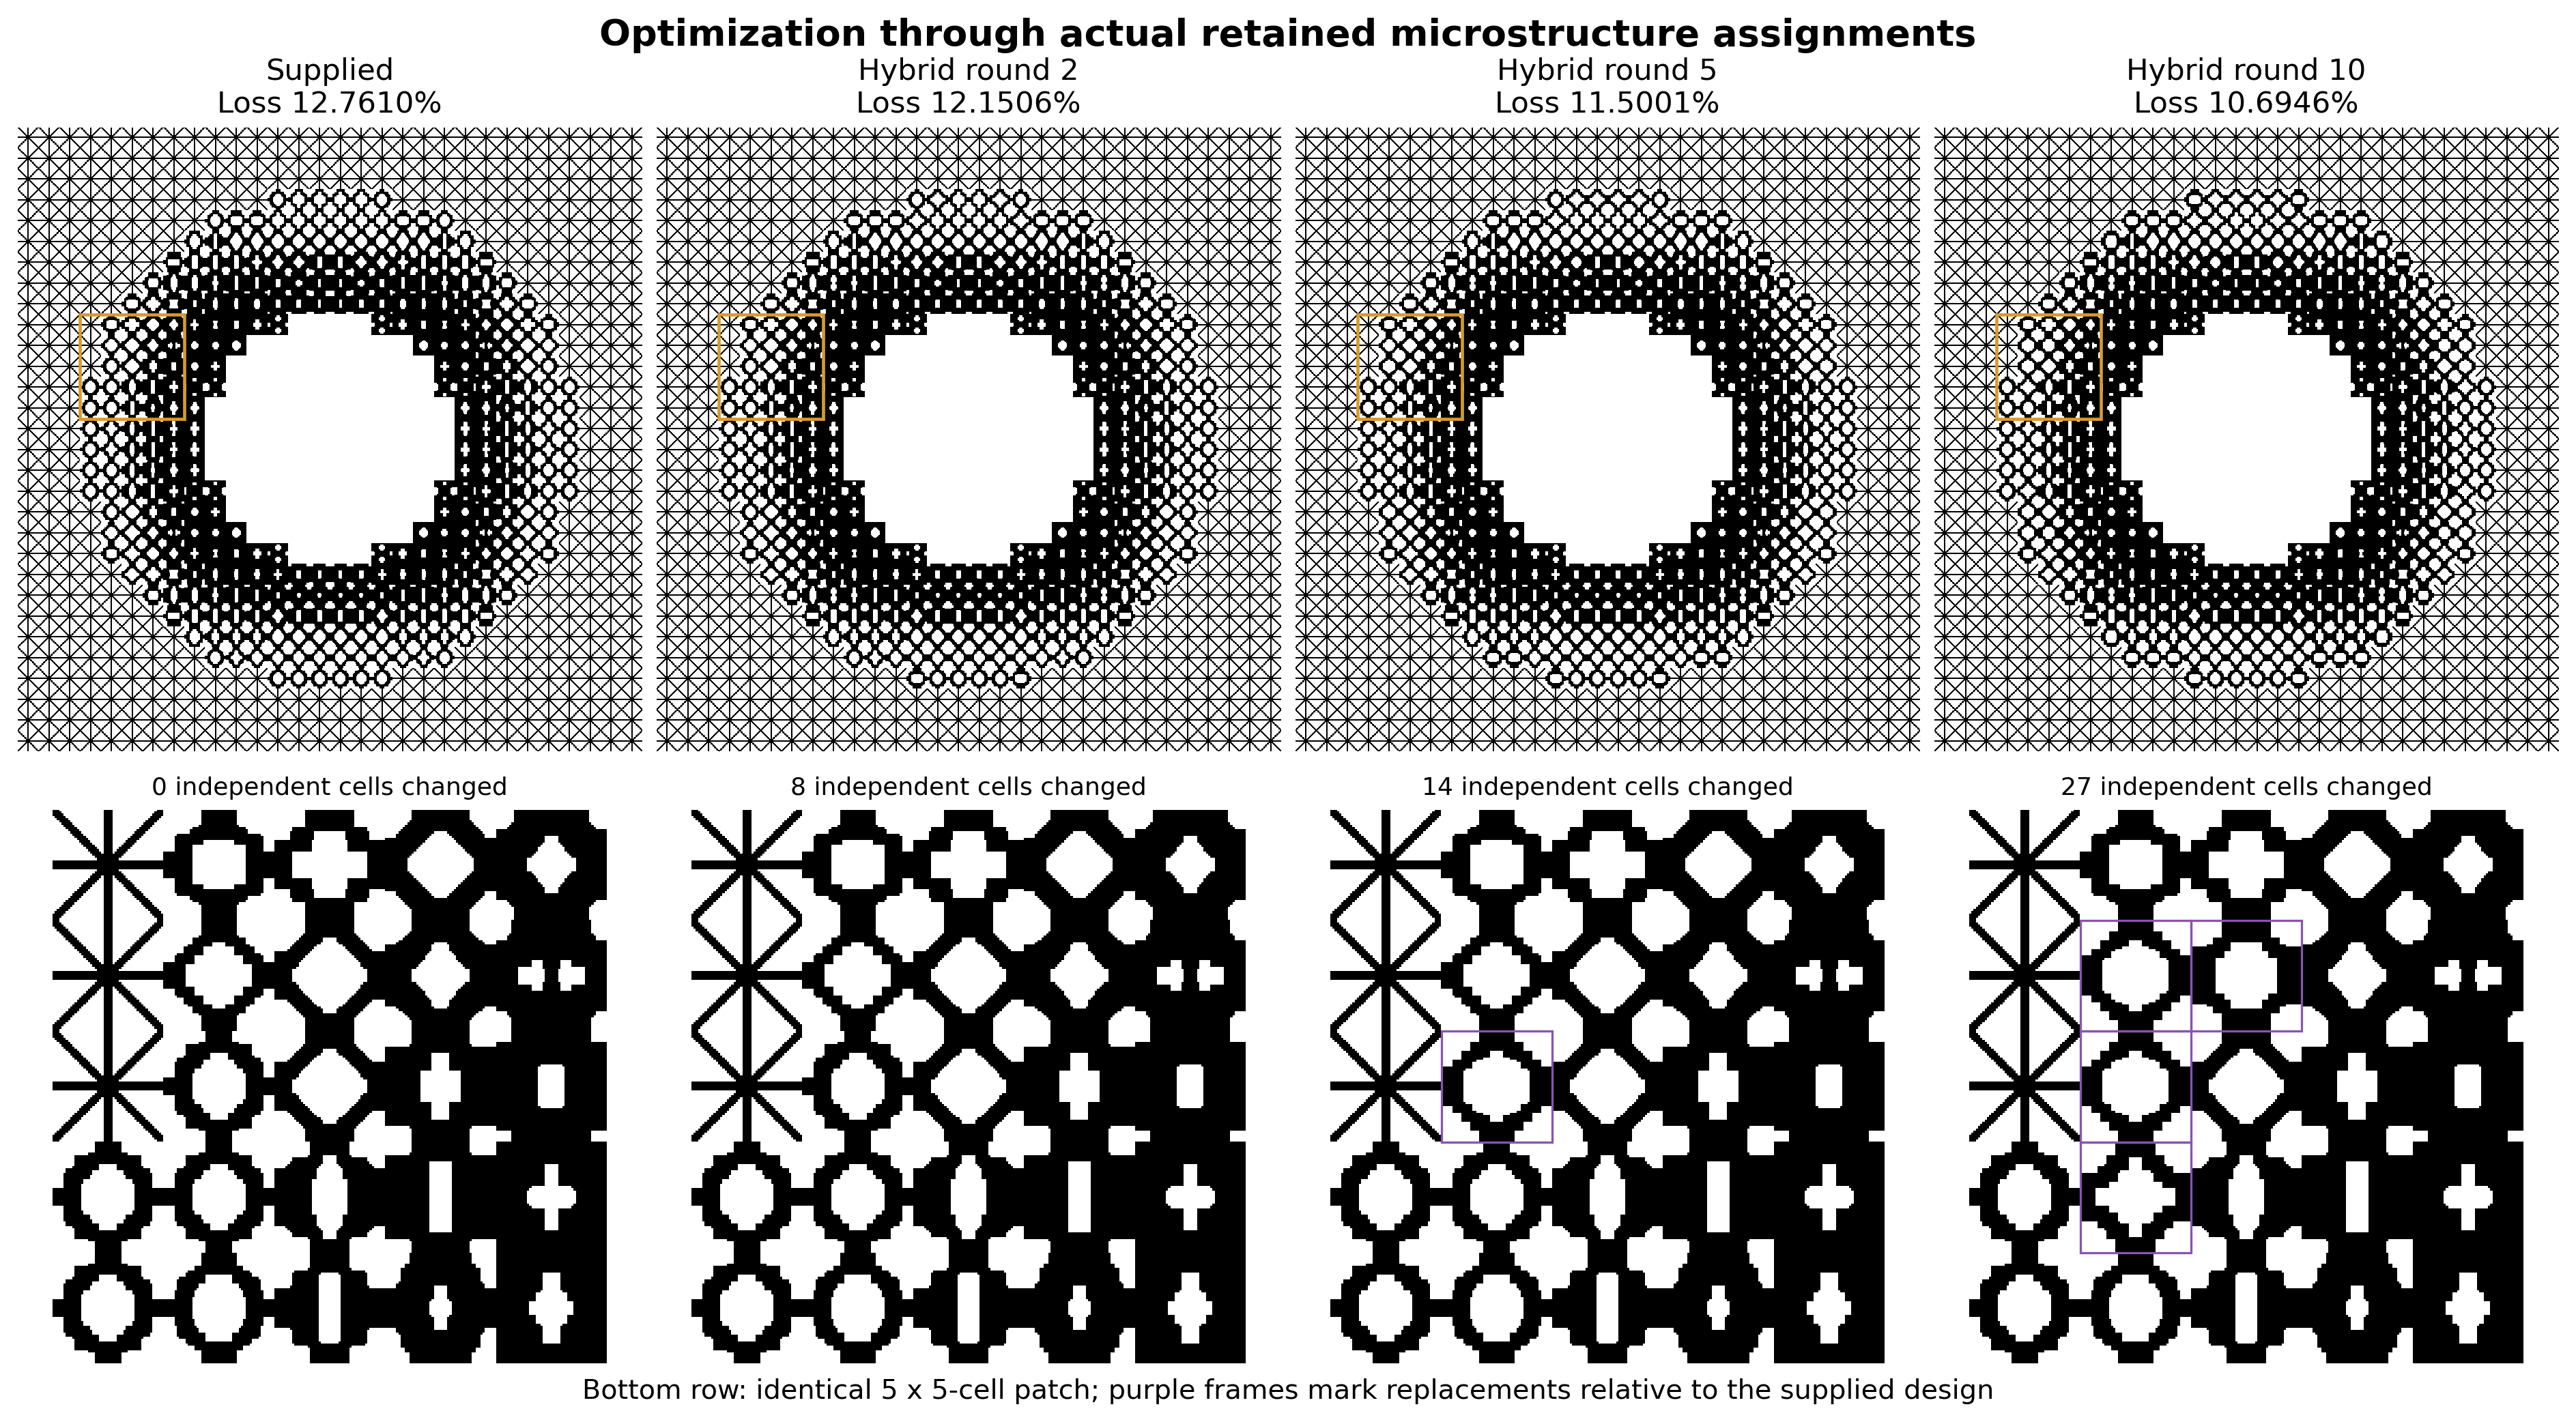
\includegraphics[width=.99\linewidth]{cloak-structure-evolution.png}}
\newcommand{\stressfields}{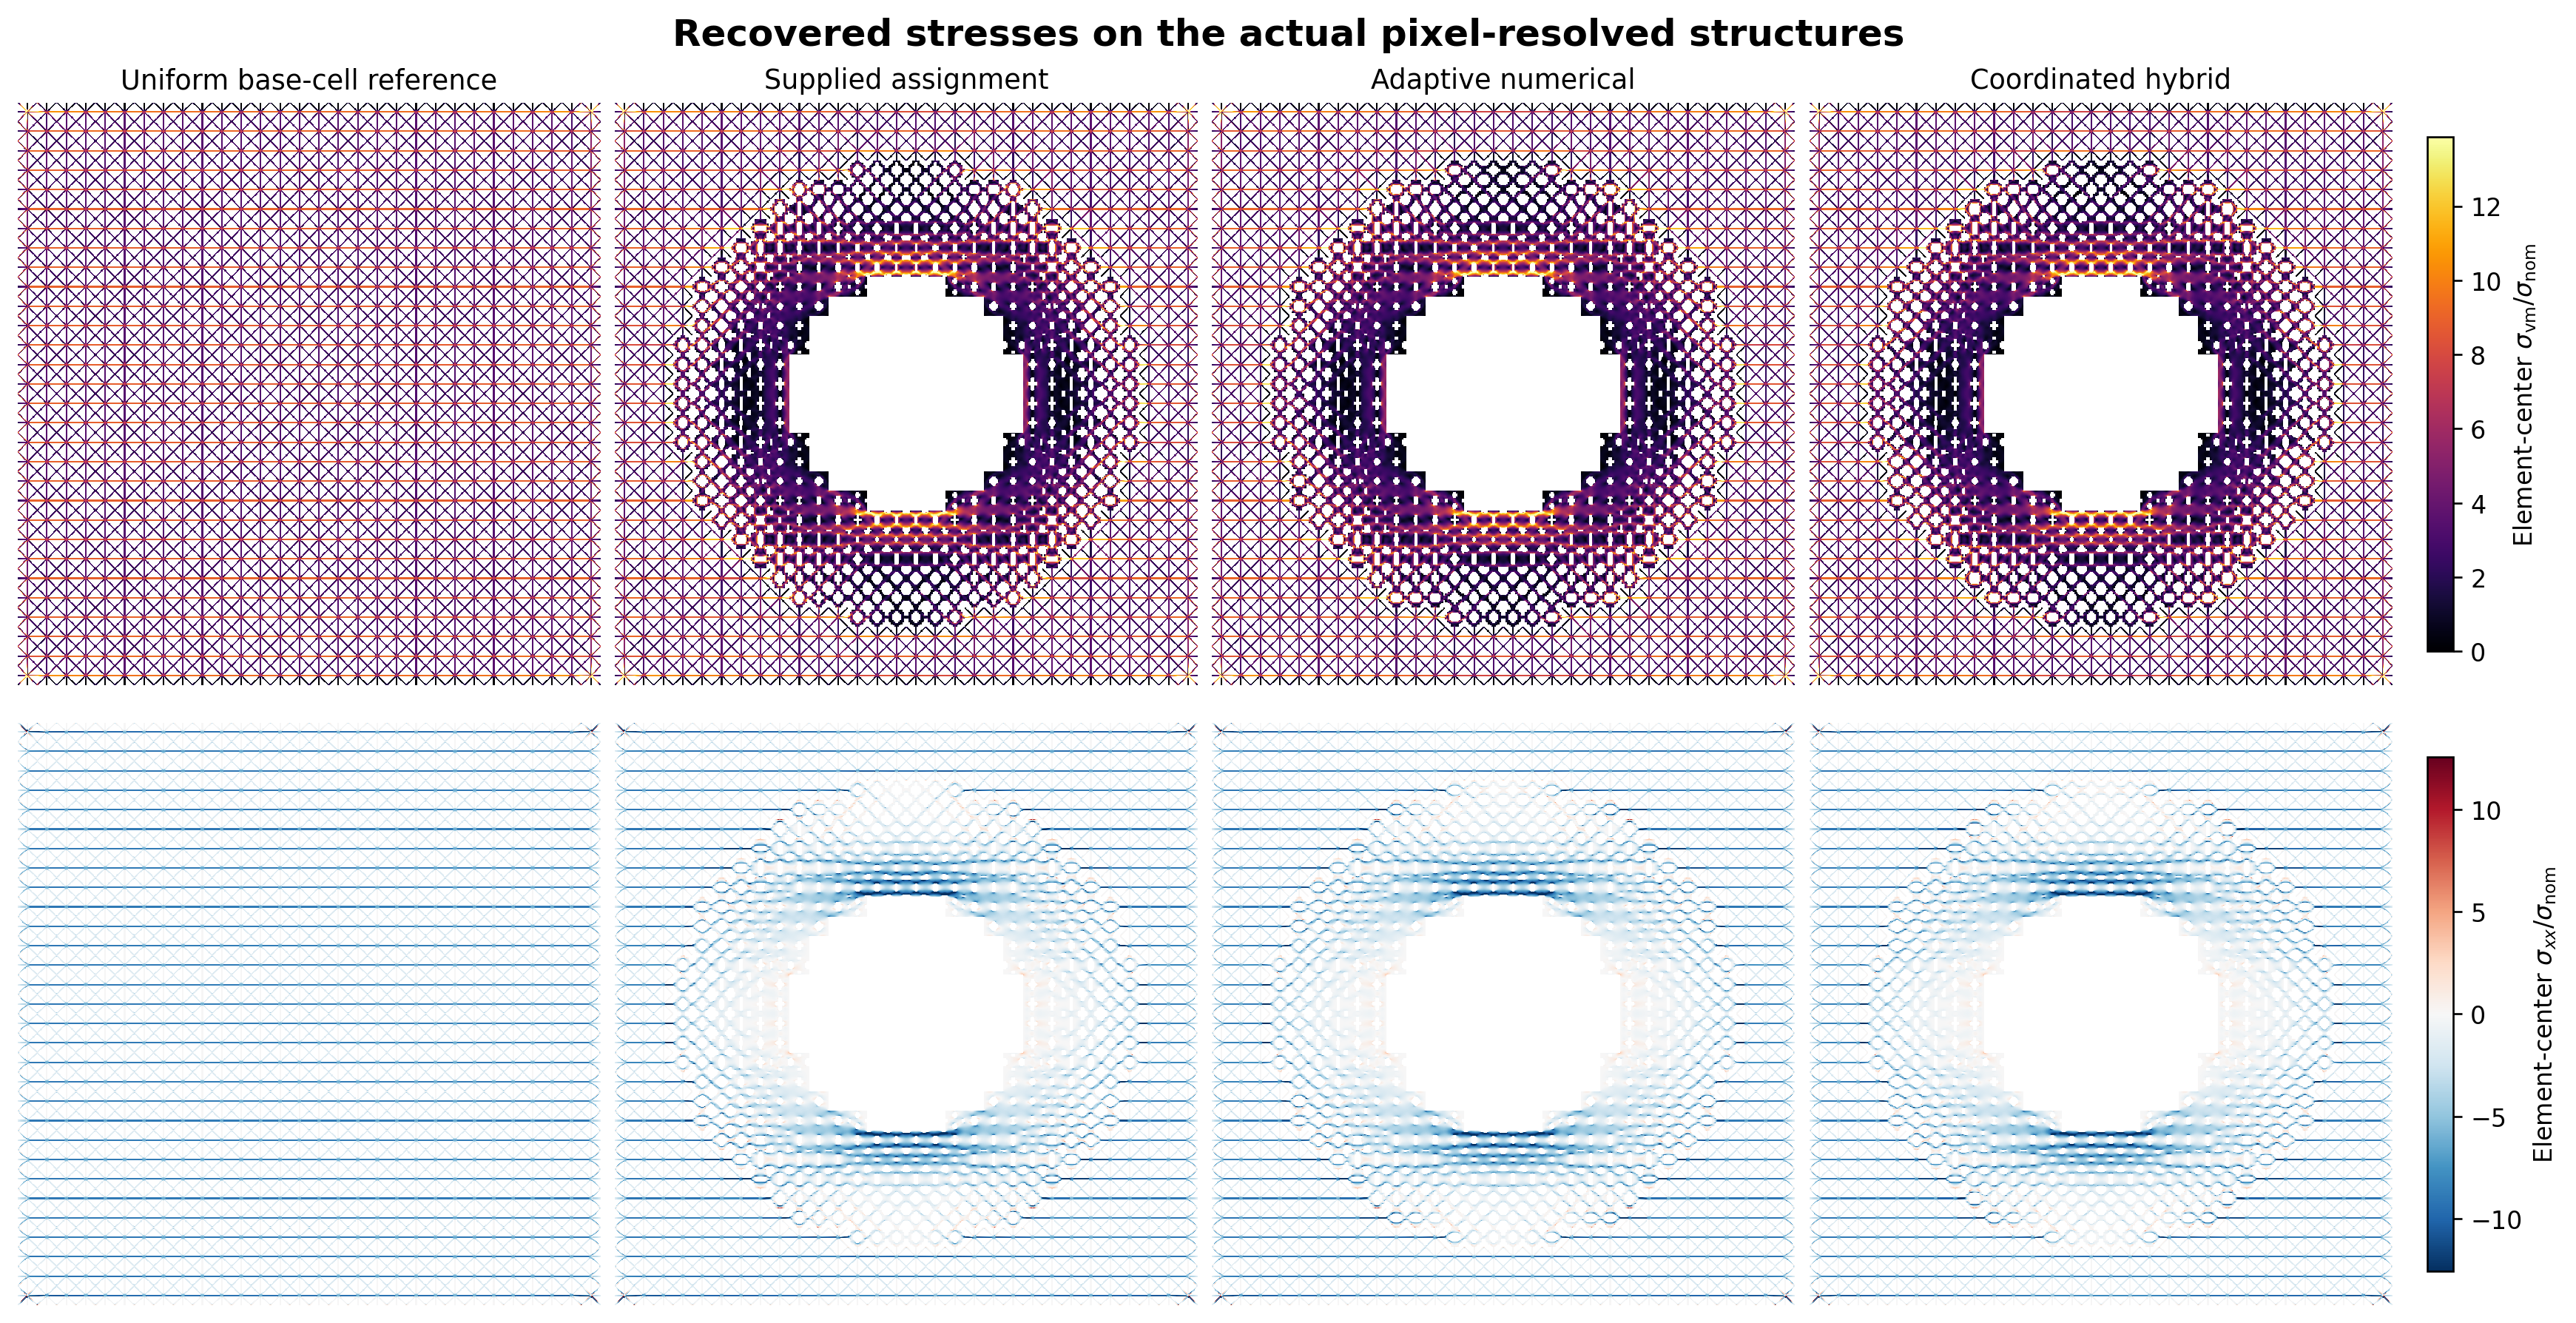
\includegraphics[width=.99\linewidth]{cloak-stress-fields.png}}
\begin{document}
\maketitle
\begin{abstract}
Selecting microstructures for a heterogeneous metamaterial is a global mechanical problem: locally suitable cells can produce an inaccurate assembled response. We investigate a coordinated search system in which language agents select existing unit-cell labels using numerical evidence and measured finite-element outcomes. A numerical proposer, response specialist, and interface specialist contribute complementary candidates; a coordinator suppresses duplicate assignments and commits proposals before evaluation. The primary case is mechanical cloaking with 168 independent selectable cells, 15 candidates per cell, and a full discretization of 2.25 million quadrilateral elements. A Python port preserves the supplied model and reproduces its monitored reference displacement to relative difference $1.29\times10^{-10}$. Starting from the same supplied assignment and identical 18-trial historical ledger, a coordinated hybrid and a frozen adaptive numerical portfolio each receive 30 new full-resolution evaluations. Masked displacement loss decreases from 12.7610\% to 10.6946\% for the hybrid and to 11.6308\% for numerical search: relative reductions of 16.19\% and 8.86\%, respectively. The hybrid's final loss is 8.05\% lower than this comparator. Matched proposal pairs document useful context-specific ablations, and final force-balance checks pass. An earlier beam experiment supplies supporting evidence, including a failed initial language-guided repair. This exploratory case supports combining agent coordination with numerical optimization; it does not establish general superiority, isolate the causal effect of coordination, or replace mechanical validation.
\end{abstract}
\noindent\textbf{Keywords:} metamaterial assembly; mechanical cloaking; language agents; discrete optimization; finite elements; experimental coordination.

\section{Introduction}
Heterogeneous mechanical metamaterials distribute different microstructures across a domain to produce a desired structural response. A unit-cell library turns topology generation into a discrete assembly problem, but the resulting design remains globally coupled through equilibrium. Neighboring cells must transmit deformation, and a close match to a target constitutive tensor does not guarantee a close match to the target displacement field.

Data-driven design frameworks already combine learned microstructure representations, property optimization, and compatibility-aware assembly~\cite{wang2020}. Database-driven aperiodic tiling has also been demonstrated for mechanical cloaks~\cite{cloak2022}. These methods motivate a narrower question: can language agents help select and repair an assembly when candidate geometries, loading, and an objective are already defined? We study selection among existing geometries. We do not retrain a generative model, generate new topologies, or ask a language model to replace the equilibrium solver.

The proposed system treats coordination as an experimental-design task. A numerical tool nominates a repair from calibrated surrogate scores. A response agent combines useful changes and proposes informative ablations. An interface agent examines neighboring geometries and tests compatible groups. The coordinator checks novelty and action validity, then commits three proposals before their measured outcomes are available. Full-resolution finite elements determine which proposal, if any, becomes the next incumbent. The shared ledger retains successes and failures so that subsequent proposals can test specific explanations rather than merely repeat promising-looking scores.

The primary evidence is a mechanical-cloaking case supplied with an assignment, candidate sets, target displacement, and MATLAB evaluator. We first audit its conventions and validate a memory-conscious Python port. We then compare independent hybrid and numerical trajectories at 30 new candidate evaluations each, with the same initial design and the same archived trial history. The hybrid reaches 10.6946\% masked displacement loss, compared with 11.6308\% for the specified adaptive numerical comparator. Figure~\ref{fig:workflow} summarizes the implemented system.

The contributions are (i) an auditable discrete cloaking benchmark at the supplied pixel resolution, (ii) a coordinated proposal protocol combining numerical repair, empirical response reasoning, and interface reasoning, and (iii) complete measured trajectories with matched proposal contrasts and numerical checks. These are contributions of an exploratory computational study. We do not claim a new constitutive theory, global optimality, the first use of language models in metamaterial design, or superiority over the original published design algorithms.


\begin{figure}[p]
\centering
\resizebox{.99\linewidth}{!}{%
% Generated from the same scene as figure1-coordinated-workflow.svg
\definecolor{figc0}{HTML}{168C88}
\definecolor{figc1}{HTML}{193248}
\definecolor{figc2}{HTML}{227DA9}
\definecolor{figc3}{HTML}{298367}
\definecolor{figc4}{HTML}{4E93B4}
\definecolor{figc5}{HTML}{526777}
\definecolor{figc6}{HTML}{88BACA}
\definecolor{figc7}{HTML}{8954B0}
\definecolor{figc8}{HTML}{BEDDE8}
\definecolor{figc9}{HTML}{C68A29}
\definecolor{figc10}{HTML}{CBD8DF}
\definecolor{figc11}{HTML}{E5F1F4}
\definecolor{figc12}{HTML}{EDF7F2}
\definecolor{figc13}{HTML}{F4F8FA}
\definecolor{figc14}{HTML}{FFFFFF}
\begin{tikzpicture}[x=1cm,y=1cm]
\node[anchor=west,text=figc1,rotate=0,font=\sffamily\bfseries\fontsize{10.00}{12.00}\selectfont,inner sep=0pt] at (0.2500,13.5500) {A   DISCRETIZED METAMATERIAL DESIGN};
\draw[fill=figc13,draw=figc10,line width=0.80pt,rounded corners=0.150cm] (0.2500,10.2500) rectangle (4.3000,13.1200);
\draw[fill=figc13,draw=figc10,line width=0.80pt,rounded corners=0.150cm] (4.9000,10.2500) rectangle (11.1000,13.1200);
\draw[fill=figc13,draw=figc10,line width=0.80pt,rounded corners=0.150cm] (11.7000,10.2500) rectangle (15.7500,13.1200);
\node[anchor=center,text=figc1,rotate=0,font=\sffamily\bfseries\fontsize{8.80}{10.56}\selectfont,inner sep=0pt] at (2.2750,12.7800) {CANDIDATE LIBRARY};
\draw[fill=figc14,draw=figc2,line width=0.80pt,rounded corners=0.025cm] (0.7350,11.3350) rectangle (1.5650,12.1650);
\draw[draw=figc2,line width=1.20pt] (1.1500,11.4014) -- (1.4986,11.7500) -- (1.1500,12.0986) -- (0.8014,11.7500) -- (1.1500,11.4014);
\draw[draw=figc2,line width=0.65pt] (0.7350,11.3350) -- (0.9757,11.5757);
\draw[draw=figc2,line width=0.65pt] (0.7350,12.1650) -- (0.9757,11.9243);
\draw[draw=figc2,line width=0.65pt] (1.5650,11.3350) -- (1.3243,11.5757);
\draw[draw=figc2,line width=0.65pt] (1.5650,12.1650) -- (1.3243,11.9243);
\draw[fill=figc14,draw=figc7,line width=0.80pt,rounded corners=0.025cm] (1.8350,11.3350) rectangle (2.6650,12.1650);
\draw[fill=figc14,draw=figc7,line width=1.20pt] (2.2500,11.7500) circle (0.2158cm);
\draw[draw=figc7,line width=1.10pt] (1.8350,11.7500) -- (2.0342,11.7500);
\draw[draw=figc7,line width=1.10pt] (2.4658,11.7500) -- (2.6650,11.7500);
\draw[draw=figc7,line width=1.10pt] (2.2500,11.3350) -- (2.2500,11.5342);
\draw[draw=figc7,line width=1.10pt] (2.2500,11.9658) -- (2.2500,12.1650);
\draw[fill=figc14,draw=figc0,line width=0.80pt,rounded corners=0.025cm] (2.9350,11.3350) rectangle (3.7650,12.1650);
\draw[draw=figc0,line width=1.10pt] (2.9350,11.3350) -- (3.7650,12.1650);
\draw[draw=figc0,line width=1.10pt] (2.9350,12.1650) -- (3.7650,11.3350);
\node[anchor=center,text=figc1,rotate=0,font=\sffamily\fontsize{8.00}{9.60}\selectfont,inner sep=0pt] at (2.2750,10.8800) {90,245 stored unit cells};
\node[anchor=center,text=figc5,rotate=0,font=\sffamily\fontsize{7.50}{9.00}\selectfont,inner sep=0pt] at (2.2750,10.5000) {15 choices at each active cell};
\draw[fill=figc14,draw=figc10,line width=0.35pt,rounded corners=0.000cm] (7.0600,10.7900) rectangle (7.2167,10.9467);
\draw[fill=figc14,draw=figc10,line width=0.35pt,rounded corners=0.000cm] (7.2167,10.7900) rectangle (7.3733,10.9467);
\draw[fill=figc14,draw=figc10,line width=0.35pt,rounded corners=0.000cm] (7.3733,10.7900) rectangle (7.5300,10.9467);
\draw[fill=figc14,draw=figc10,line width=0.35pt,rounded corners=0.000cm] (7.5300,10.7900) rectangle (7.6867,10.9467);
\draw[fill=figc14,draw=figc10,line width=0.35pt,rounded corners=0.000cm] (7.6867,10.7900) rectangle (7.8433,10.9467);
\draw[fill=figc14,draw=figc10,line width=0.35pt,rounded corners=0.000cm] (7.8433,10.7900) rectangle (8.0000,10.9467);
\draw[fill=figc14,draw=figc10,line width=0.35pt,rounded corners=0.000cm] (8.0000,10.7900) rectangle (8.1567,10.9467);
\draw[fill=figc14,draw=figc10,line width=0.35pt,rounded corners=0.000cm] (8.1567,10.7900) rectangle (8.3133,10.9467);
\draw[fill=figc14,draw=figc10,line width=0.35pt,rounded corners=0.000cm] (8.3133,10.7900) rectangle (8.4700,10.9467);
\draw[fill=figc14,draw=figc10,line width=0.35pt,rounded corners=0.000cm] (8.4700,10.7900) rectangle (8.6267,10.9467);
\draw[fill=figc14,draw=figc10,line width=0.35pt,rounded corners=0.000cm] (8.6267,10.7900) rectangle (8.7833,10.9467);
\draw[fill=figc14,draw=figc10,line width=0.35pt,rounded corners=0.000cm] (8.7833,10.7900) rectangle (8.9400,10.9467);
\draw[fill=figc14,draw=figc10,line width=0.35pt,rounded corners=0.000cm] (7.0600,10.9467) rectangle (7.2167,11.1033);
\draw[fill=figc14,draw=figc10,line width=0.35pt,rounded corners=0.000cm] (7.2167,10.9467) rectangle (7.3733,11.1033);
\draw[fill=figc14,draw=figc10,line width=0.35pt,rounded corners=0.000cm] (7.3733,10.9467) rectangle (7.5300,11.1033);
\draw[fill=figc14,draw=figc10,line width=0.35pt,rounded corners=0.000cm] (7.5300,10.9467) rectangle (7.6867,11.1033);
\draw[fill=figc14,draw=figc10,line width=0.35pt,rounded corners=0.000cm] (7.6867,10.9467) rectangle (7.8433,11.1033);
\draw[fill=figc14,draw=figc9,line width=0.35pt,rounded corners=0.000cm] (7.8433,10.9467) rectangle (8.0000,11.1033);
\draw[draw=figc9,line width=0.35pt] (7.8433,10.9467) -- (8.0000,11.1033);
\draw[fill=figc14,draw=figc2,line width=0.35pt,rounded corners=0.000cm] (8.0000,10.9467) rectangle (8.1567,11.1033);
\draw[draw=figc2,line width=0.35pt] (8.0000,10.9467) -- (8.1567,11.1033);
\draw[fill=figc14,draw=figc10,line width=0.35pt,rounded corners=0.000cm] (8.1567,10.9467) rectangle (8.3133,11.1033);
\draw[fill=figc14,draw=figc10,line width=0.35pt,rounded corners=0.000cm] (8.3133,10.9467) rectangle (8.4700,11.1033);
\draw[fill=figc14,draw=figc10,line width=0.35pt,rounded corners=0.000cm] (8.4700,10.9467) rectangle (8.6267,11.1033);
\draw[fill=figc14,draw=figc10,line width=0.35pt,rounded corners=0.000cm] (8.6267,10.9467) rectangle (8.7833,11.1033);
\draw[fill=figc14,draw=figc10,line width=0.35pt,rounded corners=0.000cm] (8.7833,10.9467) rectangle (8.9400,11.1033);
\draw[fill=figc14,draw=figc10,line width=0.35pt,rounded corners=0.000cm] (7.0600,11.1033) rectangle (7.2167,11.2600);
\draw[fill=figc14,draw=figc10,line width=0.35pt,rounded corners=0.000cm] (7.2167,11.1033) rectangle (7.3733,11.2600);
\draw[fill=figc14,draw=figc10,line width=0.35pt,rounded corners=0.000cm] (7.3733,11.1033) rectangle (7.5300,11.2600);
\draw[fill=figc14,draw=figc9,line width=0.35pt,rounded corners=0.000cm] (7.5300,11.1033) rectangle (7.6867,11.2600);
\draw[draw=figc9,line width=0.35pt] (7.5300,11.1033) -- (7.6867,11.2600);
\draw[fill=figc14,draw=figc2,line width=0.35pt,rounded corners=0.000cm] (7.6867,11.1033) rectangle (7.8433,11.2600);
\draw[draw=figc2,line width=0.35pt] (7.6867,11.1033) -- (7.8433,11.2600);
\draw[fill=figc14,draw=figc0,line width=0.35pt,rounded corners=0.000cm] (7.8433,11.1033) rectangle (8.0000,11.2600);
\draw[draw=figc0,line width=0.35pt] (7.8433,11.1033) -- (8.0000,11.2600);
\draw[fill=figc14,draw=figc7,line width=0.35pt,rounded corners=0.000cm] (8.0000,11.1033) rectangle (8.1567,11.2600);
\draw[draw=figc7,line width=0.35pt] (8.0000,11.1033) -- (8.1567,11.2600);
\draw[fill=figc14,draw=figc9,line width=0.35pt,rounded corners=0.000cm] (8.1567,11.1033) rectangle (8.3133,11.2600);
\draw[draw=figc9,line width=0.35pt] (8.1567,11.1033) -- (8.3133,11.2600);
\draw[fill=figc14,draw=figc2,line width=0.35pt,rounded corners=0.000cm] (8.3133,11.1033) rectangle (8.4700,11.2600);
\draw[draw=figc2,line width=0.35pt] (8.3133,11.1033) -- (8.4700,11.2600);
\draw[fill=figc14,draw=figc10,line width=0.35pt,rounded corners=0.000cm] (8.4700,11.1033) rectangle (8.6267,11.2600);
\draw[fill=figc14,draw=figc10,line width=0.35pt,rounded corners=0.000cm] (8.6267,11.1033) rectangle (8.7833,11.2600);
\draw[fill=figc14,draw=figc10,line width=0.35pt,rounded corners=0.000cm] (8.7833,11.1033) rectangle (8.9400,11.2600);
\draw[fill=figc14,draw=figc10,line width=0.35pt,rounded corners=0.000cm] (7.0600,11.2600) rectangle (7.2167,11.4167);
\draw[fill=figc14,draw=figc10,line width=0.35pt,rounded corners=0.000cm] (7.2167,11.2600) rectangle (7.3733,11.4167);
\draw[fill=figc14,draw=figc2,line width=0.35pt,rounded corners=0.000cm] (7.3733,11.2600) rectangle (7.5300,11.4167);
\draw[draw=figc2,line width=0.35pt] (7.3733,11.2600) -- (7.5300,11.4167);
\draw[fill=figc14,draw=figc0,line width=0.35pt,rounded corners=0.000cm] (7.5300,11.2600) rectangle (7.6867,11.4167);
\draw[draw=figc0,line width=0.35pt] (7.5300,11.2600) -- (7.6867,11.4167);
\draw[fill=figc14,draw=figc7,line width=0.35pt,rounded corners=0.000cm] (7.6867,11.2600) rectangle (7.8433,11.4167);
\draw[draw=figc7,line width=0.35pt] (7.6867,11.2600) -- (7.8433,11.4167);
\draw[fill=figc14,draw=figc9,line width=0.35pt,rounded corners=0.000cm] (7.8433,11.2600) rectangle (8.0000,11.4167);
\draw[draw=figc9,line width=0.35pt] (7.8433,11.2600) -- (8.0000,11.4167);
\draw[fill=figc14,draw=figc2,line width=0.35pt,rounded corners=0.000cm] (8.0000,11.2600) rectangle (8.1567,11.4167);
\draw[draw=figc2,line width=0.35pt] (8.0000,11.2600) -- (8.1567,11.4167);
\draw[fill=figc14,draw=figc0,line width=0.35pt,rounded corners=0.000cm] (8.1567,11.2600) rectangle (8.3133,11.4167);
\draw[draw=figc0,line width=0.35pt] (8.1567,11.2600) -- (8.3133,11.4167);
\draw[fill=figc14,draw=figc7,line width=0.35pt,rounded corners=0.000cm] (8.3133,11.2600) rectangle (8.4700,11.4167);
\draw[draw=figc7,line width=0.35pt] (8.3133,11.2600) -- (8.4700,11.4167);
\draw[fill=figc14,draw=figc9,line width=0.35pt,rounded corners=0.000cm] (8.4700,11.2600) rectangle (8.6267,11.4167);
\draw[draw=figc9,line width=0.35pt] (8.4700,11.2600) -- (8.6267,11.4167);
\draw[fill=figc14,draw=figc10,line width=0.35pt,rounded corners=0.000cm] (8.6267,11.2600) rectangle (8.7833,11.4167);
\draw[fill=figc14,draw=figc10,line width=0.35pt,rounded corners=0.000cm] (8.7833,11.2600) rectangle (8.9400,11.4167);
\draw[fill=figc14,draw=figc10,line width=0.35pt,rounded corners=0.000cm] (7.0600,11.4167) rectangle (7.2167,11.5733);
\draw[fill=figc14,draw=figc10,line width=0.35pt,rounded corners=0.000cm] (7.2167,11.4167) rectangle (7.3733,11.5733);
\draw[fill=figc14,draw=figc7,line width=0.35pt,rounded corners=0.000cm] (7.3733,11.4167) rectangle (7.5300,11.5733);
\draw[draw=figc7,line width=0.35pt] (7.3733,11.4167) -- (7.5300,11.5733);
\draw[fill=figc14,draw=figc9,line width=0.35pt,rounded corners=0.000cm] (7.5300,11.4167) rectangle (7.6867,11.5733);
\draw[draw=figc9,line width=0.35pt] (7.5300,11.4167) -- (7.6867,11.5733);
\draw[fill=figc14,draw=figc2,line width=0.35pt,rounded corners=0.000cm] (7.6867,11.4167) rectangle (7.8433,11.5733);
\draw[draw=figc2,line width=0.35pt] (7.6867,11.4167) -- (7.8433,11.5733);
\draw[fill=figc14,draw=figc9,line width=0.35pt,rounded corners=0.000cm] (8.1567,11.4167) rectangle (8.3133,11.5733);
\draw[draw=figc9,line width=0.35pt] (8.1567,11.4167) -- (8.3133,11.5733);
\draw[fill=figc14,draw=figc2,line width=0.35pt,rounded corners=0.000cm] (8.3133,11.4167) rectangle (8.4700,11.5733);
\draw[draw=figc2,line width=0.35pt] (8.3133,11.4167) -- (8.4700,11.5733);
\draw[fill=figc14,draw=figc0,line width=0.35pt,rounded corners=0.000cm] (8.4700,11.4167) rectangle (8.6267,11.5733);
\draw[draw=figc0,line width=0.35pt] (8.4700,11.4167) -- (8.6267,11.5733);
\draw[fill=figc14,draw=figc10,line width=0.35pt,rounded corners=0.000cm] (8.6267,11.4167) rectangle (8.7833,11.5733);
\draw[fill=figc14,draw=figc10,line width=0.35pt,rounded corners=0.000cm] (8.7833,11.4167) rectangle (8.9400,11.5733);
\draw[fill=figc14,draw=figc10,line width=0.35pt,rounded corners=0.000cm] (7.0600,11.5733) rectangle (7.2167,11.7300);
\draw[fill=figc14,draw=figc9,line width=0.35pt,rounded corners=0.000cm] (7.2167,11.5733) rectangle (7.3733,11.7300);
\draw[draw=figc9,line width=0.35pt] (7.2167,11.5733) -- (7.3733,11.7300);
\draw[fill=figc14,draw=figc2,line width=0.35pt,rounded corners=0.000cm] (7.3733,11.5733) rectangle (7.5300,11.7300);
\draw[draw=figc2,line width=0.35pt] (7.3733,11.5733) -- (7.5300,11.7300);
\draw[fill=figc14,draw=figc0,line width=0.35pt,rounded corners=0.000cm] (7.5300,11.5733) rectangle (7.6867,11.7300);
\draw[draw=figc0,line width=0.35pt] (7.5300,11.5733) -- (7.6867,11.7300);
\draw[fill=figc14,draw=figc7,line width=0.35pt,rounded corners=0.000cm] (8.3133,11.5733) rectangle (8.4700,11.7300);
\draw[draw=figc7,line width=0.35pt] (8.3133,11.5733) -- (8.4700,11.7300);
\draw[fill=figc14,draw=figc9,line width=0.35pt,rounded corners=0.000cm] (8.4700,11.5733) rectangle (8.6267,11.7300);
\draw[draw=figc9,line width=0.35pt] (8.4700,11.5733) -- (8.6267,11.7300);
\draw[fill=figc14,draw=figc2,line width=0.35pt,rounded corners=0.000cm] (8.6267,11.5733) rectangle (8.7833,11.7300);
\draw[draw=figc2,line width=0.35pt] (8.6267,11.5733) -- (8.7833,11.7300);
\draw[fill=figc14,draw=figc10,line width=0.35pt,rounded corners=0.000cm] (8.7833,11.5733) rectangle (8.9400,11.7300);
\draw[fill=figc14,draw=figc10,line width=0.35pt,rounded corners=0.000cm] (7.0600,11.7300) rectangle (7.2167,11.8867);
\draw[fill=figc14,draw=figc0,line width=0.35pt,rounded corners=0.000cm] (7.2167,11.7300) rectangle (7.3733,11.8867);
\draw[draw=figc0,line width=0.35pt] (7.2167,11.7300) -- (7.3733,11.8867);
\draw[fill=figc14,draw=figc7,line width=0.35pt,rounded corners=0.000cm] (7.3733,11.7300) rectangle (7.5300,11.8867);
\draw[draw=figc7,line width=0.35pt] (7.3733,11.7300) -- (7.5300,11.8867);
\draw[fill=figc14,draw=figc9,line width=0.35pt,rounded corners=0.000cm] (7.5300,11.7300) rectangle (7.6867,11.8867);
\draw[draw=figc9,line width=0.35pt] (7.5300,11.7300) -- (7.6867,11.8867);
\draw[fill=figc14,draw=figc2,line width=0.35pt,rounded corners=0.000cm] (8.3133,11.7300) rectangle (8.4700,11.8867);
\draw[draw=figc2,line width=0.35pt] (8.3133,11.7300) -- (8.4700,11.8867);
\draw[fill=figc14,draw=figc0,line width=0.35pt,rounded corners=0.000cm] (8.4700,11.7300) rectangle (8.6267,11.8867);
\draw[draw=figc0,line width=0.35pt] (8.4700,11.7300) -- (8.6267,11.8867);
\draw[fill=figc14,draw=figc7,line width=0.35pt,rounded corners=0.000cm] (8.6267,11.7300) rectangle (8.7833,11.8867);
\draw[draw=figc7,line width=0.35pt] (8.6267,11.7300) -- (8.7833,11.8867);
\draw[fill=figc14,draw=figc10,line width=0.35pt,rounded corners=0.000cm] (8.7833,11.7300) rectangle (8.9400,11.8867);
\draw[fill=figc14,draw=figc10,line width=0.35pt,rounded corners=0.000cm] (7.0600,11.8867) rectangle (7.2167,12.0433);
\draw[fill=figc14,draw=figc10,line width=0.35pt,rounded corners=0.000cm] (7.2167,11.8867) rectangle (7.3733,12.0433);
\draw[fill=figc14,draw=figc2,line width=0.35pt,rounded corners=0.000cm] (7.3733,11.8867) rectangle (7.5300,12.0433);
\draw[draw=figc2,line width=0.35pt] (7.3733,11.8867) -- (7.5300,12.0433);
\draw[fill=figc14,draw=figc0,line width=0.35pt,rounded corners=0.000cm] (7.5300,11.8867) rectangle (7.6867,12.0433);
\draw[draw=figc0,line width=0.35pt] (7.5300,11.8867) -- (7.6867,12.0433);
\draw[fill=figc14,draw=figc7,line width=0.35pt,rounded corners=0.000cm] (7.6867,11.8867) rectangle (7.8433,12.0433);
\draw[draw=figc7,line width=0.35pt] (7.6867,11.8867) -- (7.8433,12.0433);
\draw[fill=figc14,draw=figc0,line width=0.35pt,rounded corners=0.000cm] (8.1567,11.8867) rectangle (8.3133,12.0433);
\draw[draw=figc0,line width=0.35pt] (8.1567,11.8867) -- (8.3133,12.0433);
\draw[fill=figc14,draw=figc7,line width=0.35pt,rounded corners=0.000cm] (8.3133,11.8867) rectangle (8.4700,12.0433);
\draw[draw=figc7,line width=0.35pt] (8.3133,11.8867) -- (8.4700,12.0433);
\draw[fill=figc14,draw=figc9,line width=0.35pt,rounded corners=0.000cm] (8.4700,11.8867) rectangle (8.6267,12.0433);
\draw[draw=figc9,line width=0.35pt] (8.4700,11.8867) -- (8.6267,12.0433);
\draw[fill=figc14,draw=figc10,line width=0.35pt,rounded corners=0.000cm] (8.6267,11.8867) rectangle (8.7833,12.0433);
\draw[fill=figc14,draw=figc10,line width=0.35pt,rounded corners=0.000cm] (8.7833,11.8867) rectangle (8.9400,12.0433);
\draw[fill=figc14,draw=figc10,line width=0.35pt,rounded corners=0.000cm] (7.0600,12.0433) rectangle (7.2167,12.2000);
\draw[fill=figc14,draw=figc10,line width=0.35pt,rounded corners=0.000cm] (7.2167,12.0433) rectangle (7.3733,12.2000);
\draw[fill=figc14,draw=figc7,line width=0.35pt,rounded corners=0.000cm] (7.3733,12.0433) rectangle (7.5300,12.2000);
\draw[draw=figc7,line width=0.35pt] (7.3733,12.0433) -- (7.5300,12.2000);
\draw[fill=figc14,draw=figc9,line width=0.35pt,rounded corners=0.000cm] (7.5300,12.0433) rectangle (7.6867,12.2000);
\draw[draw=figc9,line width=0.35pt] (7.5300,12.0433) -- (7.6867,12.2000);
\draw[fill=figc14,draw=figc2,line width=0.35pt,rounded corners=0.000cm] (7.6867,12.0433) rectangle (7.8433,12.2000);
\draw[draw=figc2,line width=0.35pt] (7.6867,12.0433) -- (7.8433,12.2000);
\draw[fill=figc14,draw=figc0,line width=0.35pt,rounded corners=0.000cm] (7.8433,12.0433) rectangle (8.0000,12.2000);
\draw[draw=figc0,line width=0.35pt] (7.8433,12.0433) -- (8.0000,12.2000);
\draw[fill=figc14,draw=figc7,line width=0.35pt,rounded corners=0.000cm] (8.0000,12.0433) rectangle (8.1567,12.2000);
\draw[draw=figc7,line width=0.35pt] (8.0000,12.0433) -- (8.1567,12.2000);
\draw[fill=figc14,draw=figc9,line width=0.35pt,rounded corners=0.000cm] (8.1567,12.0433) rectangle (8.3133,12.2000);
\draw[draw=figc9,line width=0.35pt] (8.1567,12.0433) -- (8.3133,12.2000);
\draw[fill=figc14,draw=figc2,line width=0.35pt,rounded corners=0.000cm] (8.3133,12.0433) rectangle (8.4700,12.2000);
\draw[draw=figc2,line width=0.35pt] (8.3133,12.0433) -- (8.4700,12.2000);
\draw[fill=figc14,draw=figc0,line width=0.35pt,rounded corners=0.000cm] (8.4700,12.0433) rectangle (8.6267,12.2000);
\draw[draw=figc0,line width=0.35pt] (8.4700,12.0433) -- (8.6267,12.2000);
\draw[fill=figc14,draw=figc10,line width=0.35pt,rounded corners=0.000cm] (8.6267,12.0433) rectangle (8.7833,12.2000);
\draw[fill=figc14,draw=figc10,line width=0.35pt,rounded corners=0.000cm] (8.7833,12.0433) rectangle (8.9400,12.2000);
\draw[fill=figc14,draw=figc10,line width=0.35pt,rounded corners=0.000cm] (7.0600,12.2000) rectangle (7.2167,12.3567);
\draw[fill=figc14,draw=figc10,line width=0.35pt,rounded corners=0.000cm] (7.2167,12.2000) rectangle (7.3733,12.3567);
\draw[fill=figc14,draw=figc10,line width=0.35pt,rounded corners=0.000cm] (7.3733,12.2000) rectangle (7.5300,12.3567);
\draw[fill=figc14,draw=figc0,line width=0.35pt,rounded corners=0.000cm] (7.5300,12.2000) rectangle (7.6867,12.3567);
\draw[draw=figc0,line width=0.35pt] (7.5300,12.2000) -- (7.6867,12.3567);
\draw[fill=figc14,draw=figc7,line width=0.35pt,rounded corners=0.000cm] (7.6867,12.2000) rectangle (7.8433,12.3567);
\draw[draw=figc7,line width=0.35pt] (7.6867,12.2000) -- (7.8433,12.3567);
\draw[fill=figc14,draw=figc9,line width=0.35pt,rounded corners=0.000cm] (7.8433,12.2000) rectangle (8.0000,12.3567);
\draw[draw=figc9,line width=0.35pt] (7.8433,12.2000) -- (8.0000,12.3567);
\draw[fill=figc14,draw=figc2,line width=0.35pt,rounded corners=0.000cm] (8.0000,12.2000) rectangle (8.1567,12.3567);
\draw[draw=figc2,line width=0.35pt] (8.0000,12.2000) -- (8.1567,12.3567);
\draw[fill=figc14,draw=figc0,line width=0.35pt,rounded corners=0.000cm] (8.1567,12.2000) rectangle (8.3133,12.3567);
\draw[draw=figc0,line width=0.35pt] (8.1567,12.2000) -- (8.3133,12.3567);
\draw[fill=figc14,draw=figc7,line width=0.35pt,rounded corners=0.000cm] (8.3133,12.2000) rectangle (8.4700,12.3567);
\draw[draw=figc7,line width=0.35pt] (8.3133,12.2000) -- (8.4700,12.3567);
\draw[fill=figc14,draw=figc10,line width=0.35pt,rounded corners=0.000cm] (8.4700,12.2000) rectangle (8.6267,12.3567);
\draw[fill=figc14,draw=figc10,line width=0.35pt,rounded corners=0.000cm] (8.6267,12.2000) rectangle (8.7833,12.3567);
\draw[fill=figc14,draw=figc10,line width=0.35pt,rounded corners=0.000cm] (8.7833,12.2000) rectangle (8.9400,12.3567);
\draw[fill=figc14,draw=figc10,line width=0.35pt,rounded corners=0.000cm] (7.0600,12.3567) rectangle (7.2167,12.5133);
\draw[fill=figc14,draw=figc10,line width=0.35pt,rounded corners=0.000cm] (7.2167,12.3567) rectangle (7.3733,12.5133);
\draw[fill=figc14,draw=figc10,line width=0.35pt,rounded corners=0.000cm] (7.3733,12.3567) rectangle (7.5300,12.5133);
\draw[fill=figc14,draw=figc10,line width=0.35pt,rounded corners=0.000cm] (7.5300,12.3567) rectangle (7.6867,12.5133);
\draw[fill=figc14,draw=figc10,line width=0.35pt,rounded corners=0.000cm] (7.6867,12.3567) rectangle (7.8433,12.5133);
\draw[fill=figc14,draw=figc0,line width=0.35pt,rounded corners=0.000cm] (7.8433,12.3567) rectangle (8.0000,12.5133);
\draw[draw=figc0,line width=0.35pt] (7.8433,12.3567) -- (8.0000,12.5133);
\draw[fill=figc14,draw=figc7,line width=0.35pt,rounded corners=0.000cm] (8.0000,12.3567) rectangle (8.1567,12.5133);
\draw[draw=figc7,line width=0.35pt] (8.0000,12.3567) -- (8.1567,12.5133);
\draw[fill=figc14,draw=figc10,line width=0.35pt,rounded corners=0.000cm] (8.1567,12.3567) rectangle (8.3133,12.5133);
\draw[fill=figc14,draw=figc10,line width=0.35pt,rounded corners=0.000cm] (8.3133,12.3567) rectangle (8.4700,12.5133);
\draw[fill=figc14,draw=figc10,line width=0.35pt,rounded corners=0.000cm] (8.4700,12.3567) rectangle (8.6267,12.5133);
\draw[fill=figc14,draw=figc10,line width=0.35pt,rounded corners=0.000cm] (8.6267,12.3567) rectangle (8.7833,12.5133);
\draw[fill=figc14,draw=figc10,line width=0.35pt,rounded corners=0.000cm] (8.7833,12.3567) rectangle (8.9400,12.5133);
\draw[fill=figc14,draw=figc10,line width=0.35pt,rounded corners=0.000cm] (7.0600,12.5133) rectangle (7.2167,12.6700);
\draw[fill=figc14,draw=figc10,line width=0.35pt,rounded corners=0.000cm] (7.2167,12.5133) rectangle (7.3733,12.6700);
\draw[fill=figc14,draw=figc10,line width=0.35pt,rounded corners=0.000cm] (7.3733,12.5133) rectangle (7.5300,12.6700);
\draw[fill=figc14,draw=figc10,line width=0.35pt,rounded corners=0.000cm] (7.5300,12.5133) rectangle (7.6867,12.6700);
\draw[fill=figc14,draw=figc10,line width=0.35pt,rounded corners=0.000cm] (7.6867,12.5133) rectangle (7.8433,12.6700);
\draw[fill=figc14,draw=figc10,line width=0.35pt,rounded corners=0.000cm] (7.8433,12.5133) rectangle (8.0000,12.6700);
\draw[fill=figc14,draw=figc10,line width=0.35pt,rounded corners=0.000cm] (8.0000,12.5133) rectangle (8.1567,12.6700);
\draw[fill=figc14,draw=figc10,line width=0.35pt,rounded corners=0.000cm] (8.1567,12.5133) rectangle (8.3133,12.6700);
\draw[fill=figc14,draw=figc10,line width=0.35pt,rounded corners=0.000cm] (8.3133,12.5133) rectangle (8.4700,12.6700);
\draw[fill=figc14,draw=figc10,line width=0.35pt,rounded corners=0.000cm] (8.4700,12.5133) rectangle (8.6267,12.6700);
\draw[fill=figc14,draw=figc10,line width=0.35pt,rounded corners=0.000cm] (8.6267,12.5133) rectangle (8.7833,12.6700);
\draw[fill=figc14,draw=figc10,line width=0.35pt,rounded corners=0.000cm] (8.7833,12.5133) rectangle (8.9400,12.6700);
\draw[draw=figc1,line width=1.00pt,-{Stealth[length=1.8mm]}] (6.5800,11.7300) -- (7.0100,11.7300);
\draw[draw=figc1,line width=1.00pt,-{Stealth[length=1.8mm]}] (9.4200,11.7300) -- (8.9900,11.7300);
\node[anchor=center,text=figc1,rotate=0,font=\sffamily\bfseries\fontsize{8.00}{9.60}\selectfont,inner sep=0pt] at (8.0000,10.5500) {168 independent cloak cells};
\node[anchor=center,text=figc1,rotate=0,font=\sffamily\bfseries\fontsize{8.80}{10.56}\selectfont,inner sep=0pt] at (13.7250,12.7800) {TARGET + LOADING};
\draw[draw=figc10,line width=0.70pt] (13.1500,11.3200) -- (13.1500,12.1700);
\draw[draw=figc10,line width=0.70pt] (13.1500,11.3200) -- (14.2500,11.3200);
\draw[draw=figc0,line width=1.30pt] (13.2000,11.4200) -- (13.2500,11.5170) -- (13.3000,11.6116) -- (13.3500,11.7015) -- (13.4000,11.7844) -- (13.4500,11.8584) -- (13.5000,11.9216) -- (13.5500,11.9724) -- (13.6000,12.0097) -- (13.6500,12.0324) -- (13.7000,12.0400) -- (13.7500,12.0324) -- (13.8000,12.0097) -- (13.8500,11.9724) -- (13.9000,11.9216) -- (13.9500,11.8584) -- (14.0000,11.7844) -- (14.0500,11.7015) -- (14.1000,11.6116) -- (14.1500,11.5170) -- (14.2000,11.4200);
\draw[draw=figc0,line width=0.80pt,dashed] (13.2000,11.3400) -- (13.2500,11.4580) -- (13.3000,11.5543) -- (13.3500,11.6250) -- (13.4000,11.6855) -- (13.4500,11.7544) -- (13.5000,11.8346) -- (13.5500,11.9088) -- (13.6000,11.9544) -- (13.6500,11.9627) -- (13.7000,11.9464) -- (13.7500,11.9274) -- (13.8000,11.9162) -- (13.8500,11.9029) -- (13.9000,11.8664) -- (13.9500,11.7947) -- (14.0000,11.6972) -- (14.0500,11.5974) -- (14.1000,11.5128) -- (14.1500,11.4407) -- (14.2000,11.3628);
\node[anchor=center,text=figc1,rotate=0,font=\sffamily\fontsize{7.80}{9.36}\selectfont,inner sep=0pt] at (13.7250,10.8800) {Match exterior displacement};
\node[anchor=center,text=figc5,rotate=0,font=\sffamily\fontsize{7.50}{9.00}\selectfont,inner sep=0pt] at (13.7250,10.5000) {Fixed mask and reference};
\draw[draw=figc2,line width=1.20pt,-{Stealth[length=1.8mm]}] (4.3100,11.7200) -- (4.8500,11.7200);
\draw[draw=figc0,line width=1.20pt,-{Stealth[length=1.8mm]}] (11.6800,11.7200) -- (11.1500,11.7200);
\node[anchor=west,text=figc1,rotate=0,font=\sffamily\bfseries\fontsize{10.00}{12.00}\selectfont,inner sep=0pt] at (0.2500,9.7200) {B   COMPLEMENTARY PROPOSALS};
\draw[fill=figc14,draw=figc2,line width=1.00pt,rounded corners=0.150cm] (0.2500,6.0000) rectangle (5.1500,9.2400);
\draw[fill=figc2,draw=figc2,line width=0.80pt,rounded corners=0.110cm] (0.2500,8.7000) rectangle (5.1500,9.2400);
\draw[fill=figc14,draw=figc7,line width=1.00pt,rounded corners=0.150cm] (5.5500,6.0000) rectangle (10.4500,9.2400);
\draw[fill=figc7,draw=figc7,line width=0.80pt,rounded corners=0.110cm] (5.5500,8.7000) rectangle (10.4500,9.2400);
\draw[fill=figc14,draw=figc0,line width=1.00pt,rounded corners=0.150cm] (10.8500,6.0000) rectangle (15.7500,9.2400);
\draw[fill=figc0,draw=figc0,line width=0.80pt,rounded corners=0.110cm] (10.8500,8.7000) rectangle (15.7500,9.2400);
\node[anchor=center,text=figc14,rotate=0,font=\sffamily\bfseries\fontsize{8.80}{10.56}\selectfont,inner sep=0pt] at (2.7000,8.9700) {NUMERICAL TOOL};
\node[anchor=center,text=figc14,rotate=0,font=\sffamily\bfseries\fontsize{8.80}{10.56}\selectfont,inner sep=0pt] at (8.0000,8.9700) {RESPONSE AGENT};
\node[anchor=center,text=figc14,rotate=0,font=\sffamily\bfseries\fontsize{8.80}{10.56}\selectfont,inner sep=0pt] at (13.3000,8.9700) {INTERFACE AGENT};
\draw[fill=figc14,draw=figc2,line width=1.10pt,rounded corners=0.120cm] (1.0500,7.1200) rectangle (2.0500,8.3600);
\draw[fill=figc13,draw=figc2,line width=0.80pt,rounded corners=0.020cm] (1.1800,7.9500) rectangle (1.9200,8.2000);
\draw[fill=figc2,draw=figc2,line width=0.80pt] (1.2600,7.3400) circle (0.0650cm);
\draw[fill=figc2,draw=figc2,line width=0.80pt] (1.2600,7.6400) circle (0.0650cm);
\draw[fill=figc2,draw=figc2,line width=0.80pt] (1.5500,7.3400) circle (0.0650cm);
\draw[fill=figc2,draw=figc2,line width=0.80pt] (1.5500,7.6400) circle (0.0650cm);
\draw[fill=figc2,draw=figc2,line width=0.80pt] (1.8400,7.3400) circle (0.0650cm);
\draw[fill=figc2,draw=figc2,line width=0.80pt] (1.8400,7.6400) circle (0.0650cm);
\draw[draw=figc10,line width=0.70pt] (3.1300,7.3200) -- (3.1300,8.1700);
\draw[draw=figc10,line width=0.70pt] (3.1300,7.3200) -- (4.2300,7.3200);
\draw[draw=figc2,line width=1.30pt] (3.1800,7.4200) -- (3.2300,7.5170) -- (3.2800,7.6116) -- (3.3300,7.7015) -- (3.3800,7.7844) -- (3.4300,7.8584) -- (3.4800,7.9216) -- (3.5300,7.9724) -- (3.5800,8.0097) -- (3.6300,8.0324) -- (3.6800,8.0400) -- (3.7300,8.0324) -- (3.7800,8.0097) -- (3.8300,7.9724) -- (3.8800,7.9216) -- (3.9300,7.8584) -- (3.9800,7.7844) -- (4.0300,7.7015) -- (4.0800,7.6116) -- (4.1300,7.5170) -- (4.1800,7.4200);
\draw[draw=figc2,line width=0.80pt,dashed] (3.1800,7.3400) -- (3.2300,7.4580) -- (3.2800,7.5543) -- (3.3300,7.6250) -- (3.3800,7.6855) -- (3.4300,7.7544) -- (3.4800,7.8346) -- (3.5300,7.9088) -- (3.5800,7.9544) -- (3.6300,7.9627) -- (3.6800,7.9464) -- (3.7300,7.9274) -- (3.7800,7.9162) -- (3.8300,7.9029) -- (3.8800,7.8664) -- (3.9300,7.7947) -- (3.9800,7.6972) -- (4.0300,7.5974) -- (4.0800,7.5128) -- (4.1300,7.4407) -- (4.1800,7.3628);
\node[anchor=center,text=figc1,rotate=0,font=\sffamily\bfseries\fontsize{8.30}{9.96}\selectfont,inner sep=0pt] at (2.7000,6.6500) {Calibrate scores};
\node[anchor=center,text=figc5,rotate=0,font=\sffamily\fontsize{7.70}{9.24}\selectfont,inner sep=0pt] at (2.7000,6.2900) {Nominate a numerical repair};
\draw[fill=figc14,draw=figc7,line width=0.80pt,rounded corners=0.130cm] (6.4878,7.6876) rectangle (7.2522,8.2102);
\draw[draw=figc7,line width=1.10pt] (6.8700,8.2102) -- (6.8700,8.3896);
\draw[fill=figc7,draw=figc7,line width=0.80pt] (6.8700,8.4364) circle (0.0507cm);
\draw[fill=figc7,draw=figc7,line width=0.80pt] (6.6984,7.9918) circle (0.0523cm);
\draw[fill=figc7,draw=figc7,line width=0.80pt] (7.0416,7.9918) circle (0.0523cm);
\draw[draw=figc7,line width=1.20pt] (6.7452,7.8202) -- (6.9948,7.8202);
\draw[fill=figc14,draw=figc7,line width=0.80pt,rounded corners=0.080cm] (6.6282,7.2664) rectangle (7.1118,7.6018);
\draw[fill=figc7,draw=figc7,line width=0.80pt] (6.8700,7.4536) circle (0.0663cm);
\draw[draw=figc7,line width=1.30pt] (6.6282,7.5082) -- (6.4176,7.4068);
\draw[draw=figc7,line width=1.30pt] (7.1118,7.5082) -- (7.3146,7.5940);
\draw[draw=figc7,line width=1.40pt] (6.7374,7.2664) -- (6.7374,7.0948);
\draw[draw=figc7,line width=1.40pt] (7.0026,7.2664) -- (7.0026,7.0948);
\draw[fill=figc14,draw=figc7,line width=0.80pt,rounded corners=0.025cm] (8.3700,7.5200) rectangle (8.8900,8.0400);
\draw[draw=figc7,line width=1.20pt] (8.6300,7.5616) -- (8.8484,7.7800) -- (8.6300,7.9984) -- (8.4116,7.7800) -- (8.6300,7.5616);
\draw[draw=figc7,line width=0.65pt] (8.3700,7.5200) -- (8.5208,7.6708);
\draw[draw=figc7,line width=0.65pt] (8.3700,8.0400) -- (8.5208,7.8892);
\draw[draw=figc7,line width=0.65pt] (8.8900,7.5200) -- (8.7392,7.6708);
\draw[draw=figc7,line width=0.65pt] (8.8900,8.0400) -- (8.7392,7.8892);
\draw[fill=figc14,draw=figc7,line width=0.80pt,rounded corners=0.025cm] (8.9700,7.5200) rectangle (9.4900,8.0400);
\draw[fill=figc14,draw=figc7,line width=1.20pt] (9.2300,7.7800) circle (0.1352cm);
\draw[draw=figc7,line width=1.10pt] (8.9700,7.7800) -- (9.0948,7.7800);
\draw[draw=figc7,line width=1.10pt] (9.3652,7.7800) -- (9.4900,7.7800);
\draw[draw=figc7,line width=1.10pt] (9.2300,7.5200) -- (9.2300,7.6448);
\draw[draw=figc7,line width=1.10pt] (9.2300,7.9152) -- (9.2300,8.0400);
\draw[draw=figc7,line width=1.20pt] (8.5600,7.2000) -- (8.7900,6.9900) -- (9.2500,7.3800);
\node[anchor=center,text=figc1,rotate=0,font=\sffamily\bfseries\fontsize{8.30}{9.96}\selectfont,inner sep=0pt] at (8.0000,6.6500) {Compose + ablate};
\node[anchor=center,text=figc5,rotate=0,font=\sffamily\fontsize{7.70}{9.24}\selectfont,inner sep=0pt] at (8.0000,6.2900) {Learn which changes help};
\draw[fill=figc14,draw=figc0,line width=0.80pt,rounded corners=0.130cm] (11.7178,7.6876) rectangle (12.4822,8.2102);
\draw[draw=figc0,line width=1.10pt] (12.1000,8.2102) -- (12.1000,8.3896);
\draw[fill=figc0,draw=figc0,line width=0.80pt] (12.1000,8.4364) circle (0.0507cm);
\draw[fill=figc0,draw=figc0,line width=0.80pt] (11.9284,7.9918) circle (0.0523cm);
\draw[fill=figc0,draw=figc0,line width=0.80pt] (12.2716,7.9918) circle (0.0523cm);
\draw[draw=figc0,line width=1.20pt] (11.9752,7.8202) -- (12.2248,7.8202);
\draw[fill=figc14,draw=figc0,line width=0.80pt,rounded corners=0.080cm] (11.8582,7.2664) rectangle (12.3418,7.6018);
\draw[fill=figc0,draw=figc0,line width=0.80pt] (12.1000,7.4536) circle (0.0663cm);
\draw[draw=figc0,line width=1.30pt] (11.8582,7.5082) -- (11.6476,7.4068);
\draw[draw=figc0,line width=1.30pt] (12.3418,7.5082) -- (12.5446,7.5940);
\draw[draw=figc0,line width=1.40pt] (11.9674,7.2664) -- (11.9674,7.0948);
\draw[draw=figc0,line width=1.40pt] (12.2326,7.2664) -- (12.2326,7.0948);
\draw[fill=figc14,draw=figc0,line width=0.80pt,rounded corners=0.025cm] (13.5450,7.1150) rectangle (14.1150,7.6850);
\draw[fill=figc14,draw=figc0,line width=1.20pt] (13.8300,7.4000) circle (0.1482cm);
\draw[draw=figc0,line width=1.10pt] (13.5450,7.4000) -- (13.6818,7.4000);
\draw[draw=figc0,line width=1.10pt] (13.9782,7.4000) -- (14.1150,7.4000);
\draw[draw=figc0,line width=1.10pt] (13.8300,7.1150) -- (13.8300,7.2518);
\draw[draw=figc0,line width=1.10pt] (13.8300,7.5482) -- (13.8300,7.6850);
\draw[fill=figc14,draw=figc0,line width=0.80pt,rounded corners=0.025cm] (13.5450,7.7350) rectangle (14.1150,8.3050);
\draw[fill=figc14,draw=figc0,line width=1.20pt] (13.8300,8.0200) circle (0.1482cm);
\draw[draw=figc0,line width=1.10pt] (13.5450,8.0200) -- (13.6818,8.0200);
\draw[draw=figc0,line width=1.10pt] (13.9782,8.0200) -- (14.1150,8.0200);
\draw[draw=figc0,line width=1.10pt] (13.8300,7.7350) -- (13.8300,7.8718);
\draw[draw=figc0,line width=1.10pt] (13.8300,8.1682) -- (13.8300,8.3050);
\draw[fill=figc14,draw=figc0,line width=0.80pt,rounded corners=0.025cm] (14.1650,7.1150) rectangle (14.7350,7.6850);
\draw[fill=figc14,draw=figc0,line width=1.20pt] (14.4500,7.4000) circle (0.1482cm);
\draw[draw=figc0,line width=1.10pt] (14.1650,7.4000) -- (14.3018,7.4000);
\draw[draw=figc0,line width=1.10pt] (14.5982,7.4000) -- (14.7350,7.4000);
\draw[draw=figc0,line width=1.10pt] (14.4500,7.1150) -- (14.4500,7.2518);
\draw[draw=figc0,line width=1.10pt] (14.4500,7.5482) -- (14.4500,7.6850);
\draw[fill=figc14,draw=figc0,line width=0.80pt,rounded corners=0.025cm] (14.1650,7.7350) rectangle (14.7350,8.3050);
\draw[fill=figc14,draw=figc0,line width=1.20pt] (14.4500,8.0200) circle (0.1482cm);
\draw[draw=figc0,line width=1.10pt] (14.1650,8.0200) -- (14.3018,8.0200);
\draw[draw=figc0,line width=1.10pt] (14.5982,8.0200) -- (14.7350,8.0200);
\draw[draw=figc0,line width=1.10pt] (14.4500,7.7350) -- (14.4500,7.8718);
\draw[draw=figc0,line width=1.10pt] (14.4500,8.1682) -- (14.4500,8.3050);
\draw[draw=figc9,line width=1.30pt,dashed] (14.1400,7.1500) -- (14.1400,8.3000);
\node[anchor=center,text=figc1,rotate=0,font=\sffamily\bfseries\fontsize{8.30}{9.96}\selectfont,inner sep=0pt] at (13.3000,6.6500) {Match + extend interfaces};
\node[anchor=center,text=figc5,rotate=0,font=\sffamily\fontsize{7.70}{9.24}\selectfont,inner sep=0pt] at (13.3000,6.2900) {Test compatible cell groups};
\draw[draw=figc5,line width=0.90pt,-{Stealth[length=1.8mm]}] (2.7000,9.4700) -- (2.7000,9.2700);
\draw[draw=figc5,line width=0.90pt,-{Stealth[length=1.8mm]}] (8.0000,9.4700) -- (8.0000,9.2700);
\draw[draw=figc5,line width=0.90pt,-{Stealth[length=1.8mm]}] (13.3000,9.4700) -- (13.3000,9.2700);
\draw[draw=figc5,line width=0.80pt] (8.0000,10.2200) -- (8.0000,9.4700) -- (2.7000,9.4700);
\draw[draw=figc5,line width=0.80pt] (8.0000,9.4700) -- (13.3000,9.4700);
\draw[fill=figc13,draw=figc10,line width=0.80pt,rounded corners=0.100cm] (0.6500,5.0400) rectangle (15.3500,5.6500);
\node[anchor=center,text=figc5,rotate=0,font=\sffamily\fontsize{8.00}{9.60}\selectfont,inner sep=0pt] at (7.8000,5.3500) {SHARED LOG:  incumbent  |  predictions  |  measured successes + failures};
\draw[draw=figc5,line width=0.90pt,-{Stealth[length=1.8mm]}] (2.6000,6.0000) -- (2.6000,5.6900);
\draw[draw=figc0,line width=0.75pt,-{Stealth[length=1.8mm]}] (2.8000,5.6900) -- (2.8000,6.0000);
\draw[draw=figc5,line width=0.90pt,-{Stealth[length=1.8mm]}] (7.9000,6.0000) -- (7.9000,5.6900);
\draw[draw=figc0,line width=0.75pt,-{Stealth[length=1.8mm]}] (8.1000,5.6900) -- (8.1000,6.0000);
\draw[draw=figc5,line width=0.90pt,-{Stealth[length=1.8mm]}] (13.2000,6.0000) -- (13.2000,5.6900);
\draw[draw=figc0,line width=0.75pt,-{Stealth[length=1.8mm]}] (13.4000,5.6900) -- (13.4000,6.0000);
\draw[draw=figc9,line width=1.10pt,-{Stealth[length=1.8mm]}] (4.0000,5.0300) -- (4.0000,4.6900);
\node[anchor=west,text=figc1,rotate=0,font=\sffamily\bfseries\fontsize{10.00}{12.00}\selectfont,inner sep=0pt] at (0.2500,4.8200) {C};
\draw[fill=figc13,draw=figc9,line width=1.00pt,rounded corners=0.150cm] (0.6500,2.9300) rectangle (7.3800,4.6500);
\draw[fill=figc14,draw=figc9,line width=0.80pt,rounded corners=0.130cm] (1.2464,3.6688) rectangle (1.8736,4.0976);
\draw[draw=figc9,line width=1.10pt] (1.5600,4.0976) -- (1.5600,4.2448);
\draw[fill=figc9,draw=figc9,line width=0.80pt] (1.5600,4.2832) circle (0.0416cm);
\draw[fill=figc9,draw=figc9,line width=0.80pt] (1.4192,3.9184) circle (0.0429cm);
\draw[fill=figc9,draw=figc9,line width=0.80pt] (1.7008,3.9184) circle (0.0429cm);
\draw[draw=figc9,line width=1.20pt] (1.4576,3.7776) -- (1.6624,3.7776);
\draw[fill=figc14,draw=figc9,line width=0.80pt,rounded corners=0.080cm] (1.3616,3.3232) rectangle (1.7584,3.5984);
\draw[fill=figc9,draw=figc9,line width=0.80pt] (1.5600,3.4768) circle (0.0544cm);
\draw[draw=figc9,line width=1.30pt] (1.3616,3.5216) -- (1.1888,3.4384);
\draw[draw=figc9,line width=1.30pt] (1.7584,3.5216) -- (1.9248,3.5920);
\draw[draw=figc9,line width=1.40pt] (1.4512,3.3232) -- (1.4512,3.1824);
\draw[draw=figc9,line width=1.40pt] (1.6688,3.3232) -- (1.6688,3.1824);
\node[anchor=center,text=figc1,rotate=0,font=\sffamily\bfseries\fontsize{9.20}{11.04}\selectfont,inner sep=0pt] at (4.6100,4.2400) {COORDINATOR};
\node[anchor=center,text=figc1,rotate=0,font=\sffamily\fontsize{8.30}{9.96}\selectfont,inner sep=0pt] at (4.6100,3.7700) {Diversify / validate / commit};
\node[anchor=center,text=figc5,rotate=0,font=\sffamily\fontsize{7.30}{8.76}\selectfont,inner sep=0pt] at (4.6100,3.3000) {3 fresh proposals; up to 4 swaps each};
\draw[draw=figc9,line width=1.20pt,-{Stealth[length=1.8mm]}] (7.4200,3.8000) -- (8.9600,3.8000);
\node[anchor=center,text=figc9,rotate=0,font=\sffamily\bfseries\fontsize{7.00}{8.40}\selectfont,inner sep=0pt] at (8.2000,4.2000) {HASH};
\draw[fill=figc13,draw=figc2,line width=1.00pt,rounded corners=0.150cm] (9.0000,2.9300) rectangle (15.7500,4.6500);
\draw[fill=figc11,draw=figc14,line width=0.18pt,rounded corners=0.000cm] (9.4700,3.2600) rectangle (9.6800,3.4700);
\draw[fill=figc11,draw=figc14,line width=0.18pt,rounded corners=0.000cm] (9.6800,3.2600) rectangle (9.8900,3.4700);
\draw[fill=figc8,draw=figc14,line width=0.18pt,rounded corners=0.000cm] (9.8900,3.2600) rectangle (10.1000,3.4700);
\draw[fill=figc8,draw=figc14,line width=0.18pt,rounded corners=0.000cm] (10.1000,3.2600) rectangle (10.3100,3.4700);
\draw[fill=figc6,draw=figc14,line width=0.18pt,rounded corners=0.000cm] (10.3100,3.2600) rectangle (10.5200,3.4700);
\draw[fill=figc11,draw=figc14,line width=0.18pt,rounded corners=0.000cm] (9.4700,3.4700) rectangle (9.6800,3.6800);
\draw[fill=figc8,draw=figc14,line width=0.18pt,rounded corners=0.000cm] (9.6800,3.4700) rectangle (9.8900,3.6800);
\draw[fill=figc8,draw=figc14,line width=0.18pt,rounded corners=0.000cm] (9.8900,3.4700) rectangle (10.1000,3.6800);
\draw[fill=figc6,draw=figc14,line width=0.18pt,rounded corners=0.000cm] (10.1000,3.4700) rectangle (10.3100,3.6800);
\draw[fill=figc6,draw=figc14,line width=0.18pt,rounded corners=0.000cm] (10.3100,3.4700) rectangle (10.5200,3.6800);
\draw[fill=figc8,draw=figc14,line width=0.18pt,rounded corners=0.000cm] (9.4700,3.6800) rectangle (9.6800,3.8900);
\draw[fill=figc8,draw=figc14,line width=0.18pt,rounded corners=0.000cm] (9.6800,3.6800) rectangle (9.8900,3.8900);
\draw[fill=figc6,draw=figc14,line width=0.18pt,rounded corners=0.000cm] (9.8900,3.6800) rectangle (10.1000,3.8900);
\draw[fill=figc6,draw=figc14,line width=0.18pt,rounded corners=0.000cm] (10.1000,3.6800) rectangle (10.3100,3.8900);
\draw[fill=figc4,draw=figc14,line width=0.18pt,rounded corners=0.000cm] (10.3100,3.6800) rectangle (10.5200,3.8900);
\draw[fill=figc8,draw=figc14,line width=0.18pt,rounded corners=0.000cm] (9.4700,3.8900) rectangle (9.6800,4.1000);
\draw[fill=figc6,draw=figc14,line width=0.18pt,rounded corners=0.000cm] (9.6800,3.8900) rectangle (9.8900,4.1000);
\draw[fill=figc6,draw=figc14,line width=0.18pt,rounded corners=0.000cm] (9.8900,3.8900) rectangle (10.1000,4.1000);
\draw[fill=figc4,draw=figc14,line width=0.18pt,rounded corners=0.000cm] (10.1000,3.8900) rectangle (10.3100,4.1000);
\draw[fill=figc4,draw=figc14,line width=0.18pt,rounded corners=0.000cm] (10.3100,3.8900) rectangle (10.5200,4.1000);
\draw[fill=figc6,draw=figc14,line width=0.18pt,rounded corners=0.000cm] (9.4700,4.1000) rectangle (9.6800,4.3100);
\draw[fill=figc6,draw=figc14,line width=0.18pt,rounded corners=0.000cm] (9.6800,4.1000) rectangle (9.8900,4.3100);
\draw[fill=figc4,draw=figc14,line width=0.18pt,rounded corners=0.000cm] (9.8900,4.1000) rectangle (10.1000,4.3100);
\draw[fill=figc4,draw=figc14,line width=0.18pt,rounded corners=0.000cm] (10.1000,4.1000) rectangle (10.3100,4.3100);
\draw[fill=figc2,draw=figc14,line width=0.18pt,rounded corners=0.000cm] (10.3100,4.1000) rectangle (10.5200,4.3100);
\node[anchor=center,text=figc1,rotate=0,font=\sffamily\bfseries\fontsize{8.80}{10.56}\selectfont,inner sep=0pt] at (13.1000,4.2400) {FULL-RESOLUTION FEM};
\node[anchor=center,text=figc1,rotate=0,font=\sffamily\fontsize{8.30}{9.96}\selectfont,inner sep=0pt] at (13.1000,3.7700) {Solve equilibrium};
\node[anchor=center,text=figc5,rotate=0,font=\sffamily\fontsize{7.80}{9.36}\selectfont,inner sep=0pt] at (13.1000,3.3000) {Measure the masked loss};
\draw[draw=figc2,line width=1.10pt,-{Stealth[length=1.8mm]}] (12.1000,2.9000) -- (12.1000,2.4800) -- (10.6500,2.4800) -- (10.6500,2.1900);
\draw[fill=figc12,draw=figc3,line width=1.00pt,rounded corners=0.150cm] (3.1000,0.4800) rectangle (13.0000,2.1600);
\draw[fill=figc14,draw=figc3,line width=1.00pt] (4.0700,1.9100) -- (4.5500,1.7200) -- (4.4700,1.0900) -- (4.0700,0.7700) -- (3.6700,1.0900) -- (3.5900,1.7200) -- cycle;
\draw[draw=figc3,line width=1.50pt] (3.8300,1.3500) -- (4.0100,1.1600) -- (4.3300,1.6000);
\node[anchor=center,text=figc3,rotate=0,font=\sffamily\bfseries\fontsize{9.40}{11.28}\selectfont,inner sep=0pt] at (8.4000,1.7200) {RETAIN ONLY IMPROVEMENTS};
\node[anchor=center,text=figc1,rotate=0,font=\sffamily\fontsize{8.20}{9.84}\selectfont,inner sep=0pt] at (8.4000,1.2200) {Update the design; record every outcome};
\node[anchor=center,text=figc5,rotate=0,font=\sffamily\fontsize{7.40}{8.88}\selectfont,inner sep=0pt] at (8.4000,0.7900) {10 rounds x 3 new FEM evaluations per method};
\draw[draw=figc0,line width=1.10pt,dashed,-{Stealth[length=1.8mm]}] (13.0400,1.3000) -- (16.1200,1.3000) -- (16.1200,5.3500) -- (15.4000,5.3500);
\node[anchor=center,text=figc0,rotate=90,font=\sffamily\bfseries\fontsize{7.50}{9.00}\selectfont,inner sep=0pt] at (16.4000,3.2500) {MEASURED FEEDBACK};
\end{tikzpicture}}
\caption{Overall coordinated selection algorithm. (A) A discretized cloak is populated from fixed local candidate sets, with a fixed exterior target and loading. (B) The numerical tool calibrates scores and nominates a repair; the response LLM agent proposes compositions and ablations; the interface LLM agent tests compatible cell groups and spatial extensions. The shared log carries incumbent assignments, predictions, and all measured outcomes. (C) Coordination combines agent discussion with deterministic validity and novelty checks. Three assignments are hash-committed before full-resolution FEM, and only a measured improvement can replace the incumbent. Robot symbols identify language-agent responsibilities; the calculator and FEM block identify numerical tools. Tiles, domain, curves, and mesh are schematic, not measured response fields. The depicted ten-round budget applies separately to each method; the numerical-only comparator fills all three slots with its numerical portfolio.}
\label{fig:workflow}
\end{figure}


\section{Related work and scope}
\subsection{Microstructure libraries and mechanical cloaking}
Wang et al.~\cite{wang2020} combine a variational autoencoder, property prediction, continuous target design, and graph-based assembly. Their later cloaking study~\cite{cloak2022} uses a precomputed database to fill optimized heterogeneous regions around voids. Our work retains a supplied cavity, cloak region, candidate sets, and target; it studies local label repair after those upstream choices. The public orthotropic library~\cite{dataset} provides the cell geometry and property data used in the earlier beam pilot and matches the geometry and property arrays in the supplied cloak package.

Our numerical comparator is an adaptive local-search portfolio, not the dual-decomposition Markov-random-field algorithm of Ref.~\cite{wang2020}. No trained graph neural network (GNN) selector is evaluated. Consequently, neither the beam nor cloak errors below can be presented as a direct performance improvement over those published systems or over GNNs generally.

\subsection{Language-guided search and tool use}
Optimization by prompting~\cite{opro} places evaluated solutions in the context for subsequent language-model proposals. ReAct~\cite{react} interleaves reasoning with actions and observations, while AutoGen~\cite{autogen} develops conversable multi-agent systems with tool access. These provide relevant patterns for iterative proposal and feedback. Our application adds a fixed discrete material-action space, expensive mechanical evaluation, pre-evaluation proposal commitments, and context-specific comparisons of physical edits. We use these works for positioning; the present implementation is an assistant-mediated research workflow, not an implementation or benchmark of those frameworks.

\section{Mechanical cloaking problem}
\subsection{Candidate space and assembly}
The domain contains $30\times30$ macro cells, each represented by an original $50\times50$ binary pixel geometry. The supplied indicator identifies 112 cavity cells, 336 selectable cloak cells, and 452 fixed surrounding cells. Left--right mirror symmetry leaves 168 independent selectable cells, embedded in a $26\times13$ half-domain label array. Each active cell has 15 local candidate geometries. Passive slots are excluded from the action space, giving $15^{168}$ possible assignments and 2,352 nonincumbent single-cell replacements at any incumbent.

Let $\ell_i\in\{0,\ldots,14\}$ denote the label of independent cell $i$ and $G_{i\ell_i}$ its geometry. The assembler produces a binary field $\rho(\boldsymbol\ell)$ by placing each selected geometry and its mirror into the full domain. The source library contains 90,245 geometries with four independent orthotropic stiffness components and volume fraction~\cite{dataset}. Local candidate retrieval and the cloak region are held fixed throughout the comparison.

An action is a list of at most four distinct independent-cell replacements. Each replacement automatically updates its reflected physical cell. Cell identifiers are zero-based row-major indices of the $26\times13$ half-domain array; labels are zero based. The Python adapter preserves the original assembler's geometry reversal, mirror operation, and MATLAB label permutation. Inactive zeros in the candidate-index array are not dereferenced. This mapping matters: naively flattening the supplied label array in the wrong order would change the assembled design.

\subsection{Equilibrium, loading, and the supplied scaling}
Every pixel is a four-node plane-stress quadrilateral, with two displacement components per node and Poisson's ratio $\nu=0.35$. The full model has 2,250,000 elements and 4,506,002 displacement coordinates. With constrained coordinates eliminated, equilibrium is
\begin{equation}
\mathbf K_{ff}(\rho)\mathbf u_f=\mathbf f_f-\mathbf K_{fc}\mathbf u_c.
\label{eq:equilibrium}
\end{equation}
The supplied load case applies opposed compressive horizontal edge forces: the left edge carries positive horizontal load and the right edge negative load. The total magnitude parameter is $F_A=50(50\cdot50)^2=3.125\times10^8$, distributed over 1,500 edge intervals with half weights at endpoints. Horizontal displacement is fixed along the vertical centerline. Vertical displacement is fixed at the left-edge midpoint, center, and right-edge midpoint. These are the supplied load-case conventions, not newly optimized supports.

The legacy implementation forms an element matrix with prefactor $E_0h$ and multiplies it again by $E_{\min}+\rho_e(E_0-E_{\min})$:
\begin{equation}
\mathbf K_e=E_0h\,[E_{\min}+\rho_e(E_0-E_{\min})],\widehat{\mathbf K}_e(\nu),
\quad E_0=7\times10^6,\quad E_{\min}=10^{-9},\quad h=0.01.
\label{eq:legacy}
\end{equation}
We preserve this double occurrence of $E_0$ to reproduce the supplied reference convention, rather than silently replacing it with a different material scaling. Dividing both stiffness and load by $E_0^2h$ leaves the algebraic solution unchanged and yields the normalized void ratio $E_{\min}/E_0=1.42857\times10^{-16}$. The model is therefore a highly contrasted linear ersatz-material system. The reproduction does not independently establish a physical interpretation of the legacy units.

Exact mirror symmetry permits a $750\times1500$-element half-domain solve with 2,254,502 displacement coordinates. Reflection changes the sign of horizontal displacement and preserves vertical displacement, counting the centerline once. This is a symmetry reduction of the original discretization, not spatial coarsening. Direct sparse block assembly, symmetric diagonal equilibration, smoothed-aggregation algebraic multigrid, conjugate gradients, and iterative refinement make the solve feasible in the recorded environment.

\subsection{Masked displacement objective}
The goal is to reproduce the supplied reference response in the fixed exterior solid region. Let $\mathbf P$ select the monitored displacement coordinates and let $\mathbf u^*$ be the reference displacement. We minimize
\begin{equation}
\eps(\boldsymbol\ell)=
\frac{\|\mathbf P[\mathbf u(\rho(\boldsymbol\ell))-\mathbf u^*]\|_2}
{\|\mathbf P\mathbf u^*\|_2},\qquad J=\eps^2.
\label{eq:loss}
\end{equation}
The supplied pixel interest mask is extended to nodes by duplicating its final row and column. It selects both components at 371,241 nodes, or 742,482 displacement coordinates. We preserve this exact mask rather than sampling every node outside the cloak. The supplied target contains large nearly-void displacements away from the mask; substituting an unmasked norm would define a different and misleading objective. The monitored target norm is 1.28275944.

The original supplied assignment evaluates to $\eps_0=0.12761048866882535$. No expected scalar loss was supplied with the assignment. This is the value computed by the validated Python port, not a claim of matching a previously reported MATLAB scalar objective.

\begin{table}[htbp]
\centering\small
\caption{Primary cloaking case and fixed comparison conditions.}
\label{tab:setup}
\begin{tabular}{@{}p{.48\linewidth}p{.44\linewidth}@{}}\toprule
Quantity & Value\\\midrule
Macro domain / cell pixels & $30\times30$ / $50\times50$\\
Independent active cells / local labels & 168 / 15\\
Full elements / displacement coordinates & 2,250,000 / 4,506,002\\
Half-domain displacement coordinates & 2,254,502\\
Monitored displacement coordinates & 742,482\\
Shared historical trials & 18, identical in both arms\\
New rounds / proposals per round & 10 / 3 per arm\\
New distinct FEM assessments & 30 per arm; 60 total\\
Maximum changes per proposal & Four independent cells, mirrored automatically\\
Acceptance prerequisite & Finite loss; force residual below $10^{-7}$\\
Retention & Strictly lower measured masked loss\\\bottomrule
\end{tabular}
\end{table}

\section{Shared physical evidence and numerical proposer}
\subsection{Homogenized scalar-adjoint guidance}
Both methods receive feedback from a $30\times30$ orthotropic Q4 macro model built from candidate property tensors. Fixed surrounding cells use periodic homogenization of the base cell. Reference displacements and the interest mask are sampled consistently on the macro nodes. This approximate model supplies proposal evidence; all reported cloak losses use the original pixel-resolved model.

For macro objective $\widehat J$, macro equilibrium $\widehat{\mathbf K}\widehat{\mathbf u}=\widehat{\mathbf f}$, and the corresponding constrained scalar adjoint $\widehat{\boldsymbol\lambda}$,
\begin{equation}
\widehat{\mathbf K}_{ff}^{\mathsf T}\widehat{\boldsymbol\lambda}_f
=\left(\frac{\partial\widehat J}{\partial\widehat{\mathbf u}}\right)_f,
\qquad
s_{i\ell}=\frac{J}{\widehat J}\left[-\widehat{\boldsymbol\lambda}^{\mathsf T}
\Delta\widehat{\mathbf K}_{i\ell}\widehat{\mathbf u}\right].
\label{eq:score}
\end{equation}
Here $\Delta\widehat{\mathbf K}_{i\ell}$ includes both mirrored macro cells. The factor $J/\widehat J$ aligns objective scales; it does not make a finite replacement prediction exact. A summed batch score neglects cross-swap response interactions. At the supplied assignment, macro relative error is approximately 41.15\%, compared with fine masked loss 12.76\%. This mismatch is a reason to validate every candidate, not evidence that a persuasive agent explanation should override the evaluator.

A full-resolution scalar-adjoint attempt was stopped during preliminary development because convergence was slow. Its sensitivities are not used in either cloaking comparison. The successful small-model adjoint checks below do not establish a converged fine-model adjoint. In particular, the assembled-geometry response-vector interface used in the earlier beam study is not claimed for this cloak.

\subsection{Geometry and candidate features}
Every replacement is described by its cell and label, scaled macro score $s_{i\ell}$, supplied property-mismatch feature, volume fraction, changed-pixel fraction, and exact single-swap change in whole-assembly interface cost. For binary facing edges $a,b$, the geometric mismatch is
\begin{equation}
g(a,b)=\frac{\sum_p|a_p-b_p|}{\max(1,\sum_p(a_p\lor b_p))},
\qquad
\overline g=\frac1{1740}\sum_{(i,j)\in\mathcal E}g_{ij}.
\label{eq:interfaces}
\end{equation}
The 1,740 edges are the horizontal and vertical neighboring macro-cell pairs in the full $30\times30$ domain. For adjacent simultaneous replacements, joint interface cost must be recomputed on their shared edges rather than inferred by summing single-swap changes. The specialists recorded exact sums only when affected edge neighborhoods were disjoint; the evaluated assembly always supplies the final joint metric.

Connectivity is measured by four-neighbor adjacency of solid pixels. Volume fraction is the solid-pixel fraction. In the cloak comparison these metrics are reported, not imposed as new hard constraints. This differs from the explicit eligibility bounds used in the supporting beam study.

\subsection{Frozen adaptive numerical portfolio}
The numerical-only arm uses three deterministic proposal policies: a singleton for finite-step calibration, a bounded small-combination beam search, and a diverse beam search. It adjusts a signed response-calibration factor from measured versus predicted gains in the recent ledger. Retaining the sign matters because the macro surrogate can misrank finite changes. The factor is the median of the latest six finite gain ratios, clipped to $[-2,2]$, with an absolute floor of 0.02.

Recent unsuccessful batches shrink the changed-pixel limits, aggregate pixel budget, and number of swaps; successful outcomes can expand them. Base per-cell and aggregate pixel limits are 0.20 and 0.40, with a hard action cap of four. The trust-search predicted-gain cap adapts within $[0.025J,0.40J]$. A width-64 beam searches a pool of at most 96 candidates, formed from high-utility and low-pixel alternatives. Saturated calibrated gain is penalized by pixel change, adverse geometry change, and supplied property mismatch. The diverse policy additionally discounts concentration in a single large predicted gain. Exact formulas and constants are preserved in the frozen selector source and its hash manifest.

The calibration and proposal sizes adapt to observed outcomes; the numerical policy code itself remains fixed for the new 30-evaluation experiment. We therefore call it adaptive numerical search, while distinguishing parameter adaptation from the hybrid specialists' ability to change their reasoning strategy. This is a specific local optimizer, not a comprehensive numerical-optimization benchmark.

\section{Coordinated hybrid algorithm}
\subsection{Responsibilities and communication}
The hybrid fills three evaluation slots each round. Its first slot is the singleton nominee from the same numerical optimizer used by the comparator. The response LLM specialist fills a second slot by composing measured helpful changes, proposing subsets after failures, or testing small repairs under uncertainty. The interface LLM specialist fills the third slot by examining geometric compatibility and spatially coherent groups. These two specialist roles communicate directly to avoid redundant proposals and, where useful, construct matched comparisons.

The coordinator is a workflow responsibility combining language-mediated discussion and deterministic code checks, rather than an independently benchmarked third specialist. It shares the hybrid's current assignment, scores, and measured ledger; checks active-cell eligibility, valid labels, distinct changed cells, and assignment novelty; and combines the three nominations. The full assignment after applying actions is the unit of novelty. Different action strings that produce the same design are not treated as new proposals.

Only the hybrid's own new measurements enter its subsequent feedback. It does not inspect the new numerical arm's outcomes. The numerical arm likewise does not receive the hybrid's new outcomes. The identical historical ledger is shared once at initialization. Specialists are computational roles instantiated in an assistant-mediated session, not independent statistical replicates or separately trained models.

\subsection{Commit, evaluate, retain}
At round $t$, let $\boldsymbol\ell_t$ be the incumbent, $\mathcal H_t$ the available ledger, and $\mathcal A_t=\{a_t^{\rm num},a_t^{\rm resp},a_t^{\rm int}\}$ the three action lists. The coordinator requires
\begin{equation}
1\leq |a_t^k|\leq4,\quad
i\neq j\text{ for distinct edits in }a_t^k,\quad
\rho(\boldsymbol\ell_t\oplus a_t^k)\text{ is a fresh assignment}.
\label{eq:actions}
\end{equation}
The three proposals are saved and SHA-256 hashed before any outcome from that arm and round is evaluated. Valid proposals are then assessed by fine FEM. Define eligibility as finite $\eps$ and free-force residual below $10^{-7}$. The retention rule is
\begin{equation}
\boldsymbol\ell_{t+1}\in\underset{\boldsymbol\ell\in
\{\boldsymbol\ell_t\}\cup\{\boldsymbol\ell_t\oplus a_t^k:\ k\text{ eligible}\}}
{\operatorname{argmin}}\ \eps(\boldsymbol\ell),
\label{eq:retain}
\end{equation}
with the incumbent unchanged unless the measured loss is strictly lower. All outcomes, including failed proposals, are appended to $\mathcal H_t$. Eligibility is numerical and label-space validity; it is not a manufacturing certificate.

\begin{table}[htbp]
\centering\small
\caption{Executed hybrid loop. All three nominees use the same round-starting incumbent.}
\label{tab:algorithm}
\begin{tabular}{@{}cp{.87\linewidth}@{}}\toprule
Step & Operation\\\midrule
1 & Load incumbent, identical-form macro feedback, and own-arm measured history.\\
2 & Obtain one numerical nominee and one nominee from each LLM specialist.\\
3 & Discuss complementary hypotheses; resolve duplicates before evaluation.\\
4 & Validate actions and full-assignment novelty; save and hash all three proposals.\\
5 & Solve each candidate at the original fine resolution; record loss and diagnostics.\\
6 & Retain the best eligible strict improvement; append every trial to the shared log.\\
7 & Repeat until ten rounds and 30 new fine evaluations are complete.\\\bottomrule
\end{tabular}
\end{table}

\section{Experimental design}
\subsection{Preliminary studies and the common historical ledger}
The project began with a beam pilot, followed by a more demanding author-supplied cloak. A preliminary cloak comparison used three rounds of three proposals per arm. It reduced loss from 12.7610\% to 12.3594\% for adaptive numerical search and to 12.5406\% for a three-specialist swarm. Numerical policy refinements occurred during that exploratory session, and all outcomes were retained. This preliminary result favored the numerical search; it is not omitted from the present account.

The primary coordinated follow-up restarts both methods from the original supplied assignment, rather than from either preliminary winner. Both methods receive the same 18 historical trials, including actions, incumbent contexts, predicted changes, measured losses, and failures. This treatment acknowledges that the specialists already know the earlier study; restarting an array cannot erase conversational knowledge. Previously assessed full assignments are excluded from new proposals. The follow-up is therefore a warm-history exploratory comparison, not a blinded or held-out test.

\subsection{Matched budgets and independent trajectories}
The numerical-only arm submits all three numerical portfolio nominees each round. The hybrid submits one numerical nominee and two coordinated specialist nominees. Each arm completes ten rounds with three distinct fresh candidates per round: 30 new full-resolution candidate evaluations each. Both start with $\eps_0$, but thereafter retain separate incumbents and use their own new histories. Unlike the earlier beam proposal competition, one arm's accepted design is never handed to the other arm.

All 60 new proposal records report uncached evaluations. A design shared across arms is independently solved rather than counted as a free measurement. The common baseline, historical trials, reference reconstruction, and final diagnostic checks are outside the new candidate budgets. No unreported candidate-FEM lookahead is used to select the new proposals.

Equal fine-evaluation counts control an expensive resource, not total optimization effort. Agent latency, token use, and proposal-search computation were not matched. Nor does the design isolate agent coordination from every other policy difference: the hybrid specialists can revise strategy while the numerical policy code is frozen. We report a system-level comparison of these implemented methods.

\section{Results}
\subsection{Primary matched-budget comparison}
Table~\ref{tab:primary} reports the final primary outcomes. The hybrid reduces masked loss by 16.19\% relative to the supplied assignment; numerical search reduces it by 8.86\%. The hybrid's final loss is 8.05\% lower than the numerical comparator's final loss, an absolute difference of 0.9362 percentage points. These percentages refer to the norm error $\eps$, not its square $J$.

\begin{table}[htbp]
\centering
\caption{Primary cloak outcomes after 30 new fine evaluations per method. Both use the same starting assignment and 18-trial historical ledger.}
\label{tab:primary}
\begin{tabular}{@{}lrrr@{}}\toprule
Method & New FEM tests & Loss (\%) & Relative reduction\\\midrule
Supplied assignment & --- & 12.761049 & ---\\
Adaptive numerical & 30 & 11.630822 & 8.857\%\\
Coordinated hybrid & 30 & \textbf{10.694605} & \textbf{16.193\%}\\\bottomrule
\end{tabular}
\end{table}

The retained trajectories in Fig.~\ref{fig:convergence} show different search behavior. Numerical search makes a larger improvement in round four, then continues with smaller gains. The hybrid improves its retained loss in every round. This monotonicity is guaranteed by retention for either method; the fact that every hybrid round supplies a useful candidate is an observed result, not a general property of language agents. Across all proposals, 21 of 30 numerical candidates and 20 of 30 hybrid candidates improve their own round-starting design. The hybrid advantage therefore does not reduce to a higher fraction of improving trials; the size and composition of useful changes matter.

\begin{figure}[htbp]
\centering
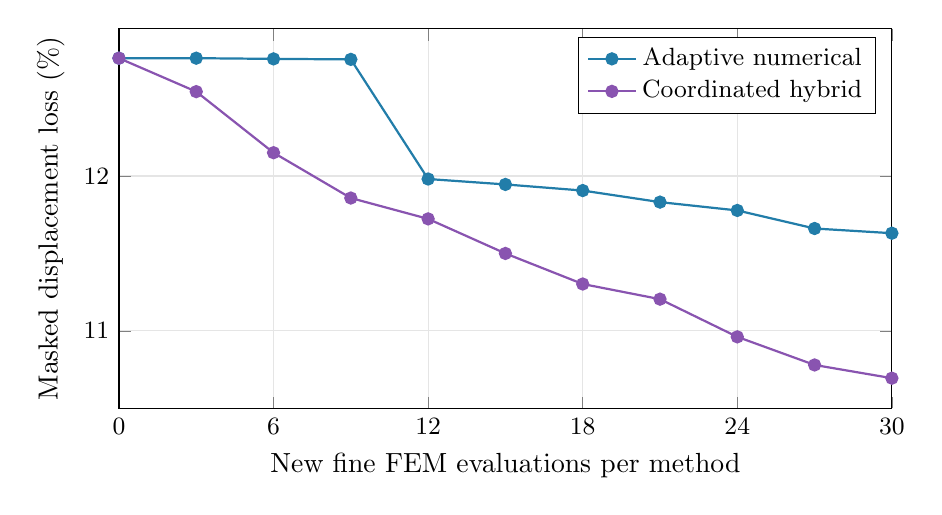
\begin{tikzpicture}
\begin{axis}[width=.94\linewidth,height=6.4cm,xlabel={New fine FEM evaluations per method},ylabel={Masked displacement loss (\%)},xmin=0,xmax=30,ymin=10.5,ymax=12.95,xtick={0,6,12,18,24,30},grid=major,grid style={black!10},legend style={at={(.98,.98)},anchor=north east,font=\small},tick label style={font=\small}]
\addplot[numblue,thick,mark=*] coordinates {(0,12.761048867) (3,12.761048867) (6,12.756484437) (9,12.753282779) (12,11.980757952) (15,11.945736169) (18,11.906258261) (21,11.831545442) (24,11.777804797) (27,11.661215919) (30,11.630822449)};
\addlegendentry{Adaptive numerical}
\addplot[agentpurple,thick,mark=*] coordinates {(0,12.761048867) (3,12.545021481) (6,12.150599530) (9,11.857962331) (12,11.723328628) (15,11.500134333) (18,11.302764112) (21,11.204944411) (24,10.961471774) (27,10.780012094) (30,10.694605291)};
\addlegendentry{Coordinated hybrid}
\end{axis}\end{tikzpicture}
\caption{Measured retained loss for the primary independent trajectories. Points mark completed three-proposal rounds. Both arms restart from the original assignment with identical historical evidence. No error bars are shown because these are single trajectories, not repeated-run estimates.}
\label{fig:convergence}
\end{figure}

\subsection{Spatial changes and secondary metrics}
The numerical and hybrid final assignments differ from the original at 18 and 27 independent cells, respectively. Both retain one four-neighbor connected solid component. Their volume fractions are 0.412736 and 0.412640, compared with 0.41096178 for the supplied assignment. Their mean geometric mismatch costs are 0.121292 and 0.118689. Figure~\ref{fig:locations} maps the changed macro cells. Figure~\ref{fig:evolution} shows actual retained pixel-resolved structures with a common magnified patch; Figs.~\ref{fig:stressfields} and~\ref{fig:stressprofiles} show stresses recovered from saved fine solutions.

The larger accumulated number of hybrid changes is compatible with the four-swap limit: the cap applies to each proposal, while successive retained proposals can alter different cells. These results do not establish equal-material optimality, since volume was not fixed as an exact constraint. Connectedness and lower interface mismatch are useful secondary observations, not proofs of strength, buckling resistance, or printability.

\begin{figure}[htbp]
\centering\resizebox{.99\linewidth}{!}{%
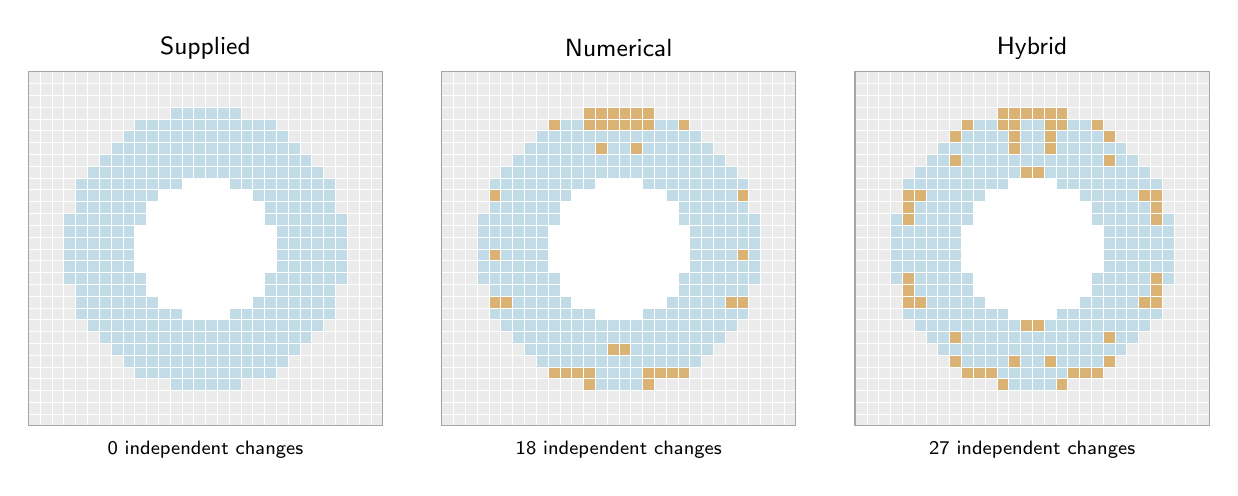
\begin{tikzpicture}[x=.15cm,y=.15cm]
\filldraw[fill=black!8,draw=white,line width=.14pt] (0,29) rectangle (1,30);
\filldraw[fill=black!8,draw=white,line width=.14pt] (1,29) rectangle (2,30);
\filldraw[fill=black!8,draw=white,line width=.14pt] (2,29) rectangle (3,30);
\filldraw[fill=black!8,draw=white,line width=.14pt] (3,29) rectangle (4,30);
\filldraw[fill=black!8,draw=white,line width=.14pt] (4,29) rectangle (5,30);
\filldraw[fill=black!8,draw=white,line width=.14pt] (5,29) rectangle (6,30);
\filldraw[fill=black!8,draw=white,line width=.14pt] (6,29) rectangle (7,30);
\filldraw[fill=black!8,draw=white,line width=.14pt] (7,29) rectangle (8,30);
\filldraw[fill=black!8,draw=white,line width=.14pt] (8,29) rectangle (9,30);
\filldraw[fill=black!8,draw=white,line width=.14pt] (9,29) rectangle (10,30);
\filldraw[fill=black!8,draw=white,line width=.14pt] (10,29) rectangle (11,30);
\filldraw[fill=black!8,draw=white,line width=.14pt] (11,29) rectangle (12,30);
\filldraw[fill=black!8,draw=white,line width=.14pt] (12,29) rectangle (13,30);
\filldraw[fill=black!8,draw=white,line width=.14pt] (13,29) rectangle (14,30);
\filldraw[fill=black!8,draw=white,line width=.14pt] (14,29) rectangle (15,30);
\filldraw[fill=black!8,draw=white,line width=.14pt] (15,29) rectangle (16,30);
\filldraw[fill=black!8,draw=white,line width=.14pt] (16,29) rectangle (17,30);
\filldraw[fill=black!8,draw=white,line width=.14pt] (17,29) rectangle (18,30);
\filldraw[fill=black!8,draw=white,line width=.14pt] (18,29) rectangle (19,30);
\filldraw[fill=black!8,draw=white,line width=.14pt] (19,29) rectangle (20,30);
\filldraw[fill=black!8,draw=white,line width=.14pt] (20,29) rectangle (21,30);
\filldraw[fill=black!8,draw=white,line width=.14pt] (21,29) rectangle (22,30);
\filldraw[fill=black!8,draw=white,line width=.14pt] (22,29) rectangle (23,30);
\filldraw[fill=black!8,draw=white,line width=.14pt] (23,29) rectangle (24,30);
\filldraw[fill=black!8,draw=white,line width=.14pt] (24,29) rectangle (25,30);
\filldraw[fill=black!8,draw=white,line width=.14pt] (25,29) rectangle (26,30);
\filldraw[fill=black!8,draw=white,line width=.14pt] (26,29) rectangle (27,30);
\filldraw[fill=black!8,draw=white,line width=.14pt] (27,29) rectangle (28,30);
\filldraw[fill=black!8,draw=white,line width=.14pt] (28,29) rectangle (29,30);
\filldraw[fill=black!8,draw=white,line width=.14pt] (29,29) rectangle (30,30);
\filldraw[fill=black!8,draw=white,line width=.14pt] (0,28) rectangle (1,29);
\filldraw[fill=black!8,draw=white,line width=.14pt] (1,28) rectangle (2,29);
\filldraw[fill=black!8,draw=white,line width=.14pt] (2,28) rectangle (3,29);
\filldraw[fill=black!8,draw=white,line width=.14pt] (3,28) rectangle (4,29);
\filldraw[fill=black!8,draw=white,line width=.14pt] (4,28) rectangle (5,29);
\filldraw[fill=black!8,draw=white,line width=.14pt] (5,28) rectangle (6,29);
\filldraw[fill=black!8,draw=white,line width=.14pt] (6,28) rectangle (7,29);
\filldraw[fill=black!8,draw=white,line width=.14pt] (7,28) rectangle (8,29);
\filldraw[fill=black!8,draw=white,line width=.14pt] (8,28) rectangle (9,29);
\filldraw[fill=black!8,draw=white,line width=.14pt] (9,28) rectangle (10,29);
\filldraw[fill=black!8,draw=white,line width=.14pt] (10,28) rectangle (11,29);
\filldraw[fill=black!8,draw=white,line width=.14pt] (11,28) rectangle (12,29);
\filldraw[fill=black!8,draw=white,line width=.14pt] (12,28) rectangle (13,29);
\filldraw[fill=black!8,draw=white,line width=.14pt] (13,28) rectangle (14,29);
\filldraw[fill=black!8,draw=white,line width=.14pt] (14,28) rectangle (15,29);
\filldraw[fill=black!8,draw=white,line width=.14pt] (15,28) rectangle (16,29);
\filldraw[fill=black!8,draw=white,line width=.14pt] (16,28) rectangle (17,29);
\filldraw[fill=black!8,draw=white,line width=.14pt] (17,28) rectangle (18,29);
\filldraw[fill=black!8,draw=white,line width=.14pt] (18,28) rectangle (19,29);
\filldraw[fill=black!8,draw=white,line width=.14pt] (19,28) rectangle (20,29);
\filldraw[fill=black!8,draw=white,line width=.14pt] (20,28) rectangle (21,29);
\filldraw[fill=black!8,draw=white,line width=.14pt] (21,28) rectangle (22,29);
\filldraw[fill=black!8,draw=white,line width=.14pt] (22,28) rectangle (23,29);
\filldraw[fill=black!8,draw=white,line width=.14pt] (23,28) rectangle (24,29);
\filldraw[fill=black!8,draw=white,line width=.14pt] (24,28) rectangle (25,29);
\filldraw[fill=black!8,draw=white,line width=.14pt] (25,28) rectangle (26,29);
\filldraw[fill=black!8,draw=white,line width=.14pt] (26,28) rectangle (27,29);
\filldraw[fill=black!8,draw=white,line width=.14pt] (27,28) rectangle (28,29);
\filldraw[fill=black!8,draw=white,line width=.14pt] (28,28) rectangle (29,29);
\filldraw[fill=black!8,draw=white,line width=.14pt] (29,28) rectangle (30,29);
\filldraw[fill=black!8,draw=white,line width=.14pt] (0,27) rectangle (1,28);
\filldraw[fill=black!8,draw=white,line width=.14pt] (1,27) rectangle (2,28);
\filldraw[fill=black!8,draw=white,line width=.14pt] (2,27) rectangle (3,28);
\filldraw[fill=black!8,draw=white,line width=.14pt] (3,27) rectangle (4,28);
\filldraw[fill=black!8,draw=white,line width=.14pt] (4,27) rectangle (5,28);
\filldraw[fill=black!8,draw=white,line width=.14pt] (5,27) rectangle (6,28);
\filldraw[fill=black!8,draw=white,line width=.14pt] (6,27) rectangle (7,28);
\filldraw[fill=black!8,draw=white,line width=.14pt] (7,27) rectangle (8,28);
\filldraw[fill=black!8,draw=white,line width=.14pt] (8,27) rectangle (9,28);
\filldraw[fill=black!8,draw=white,line width=.14pt] (9,27) rectangle (10,28);
\filldraw[fill=black!8,draw=white,line width=.14pt] (10,27) rectangle (11,28);
\filldraw[fill=black!8,draw=white,line width=.14pt] (11,27) rectangle (12,28);
\filldraw[fill=black!8,draw=white,line width=.14pt] (12,27) rectangle (13,28);
\filldraw[fill=black!8,draw=white,line width=.14pt] (13,27) rectangle (14,28);
\filldraw[fill=black!8,draw=white,line width=.14pt] (14,27) rectangle (15,28);
\filldraw[fill=black!8,draw=white,line width=.14pt] (15,27) rectangle (16,28);
\filldraw[fill=black!8,draw=white,line width=.14pt] (16,27) rectangle (17,28);
\filldraw[fill=black!8,draw=white,line width=.14pt] (17,27) rectangle (18,28);
\filldraw[fill=black!8,draw=white,line width=.14pt] (18,27) rectangle (19,28);
\filldraw[fill=black!8,draw=white,line width=.14pt] (19,27) rectangle (20,28);
\filldraw[fill=black!8,draw=white,line width=.14pt] (20,27) rectangle (21,28);
\filldraw[fill=black!8,draw=white,line width=.14pt] (21,27) rectangle (22,28);
\filldraw[fill=black!8,draw=white,line width=.14pt] (22,27) rectangle (23,28);
\filldraw[fill=black!8,draw=white,line width=.14pt] (23,27) rectangle (24,28);
\filldraw[fill=black!8,draw=white,line width=.14pt] (24,27) rectangle (25,28);
\filldraw[fill=black!8,draw=white,line width=.14pt] (25,27) rectangle (26,28);
\filldraw[fill=black!8,draw=white,line width=.14pt] (26,27) rectangle (27,28);
\filldraw[fill=black!8,draw=white,line width=.14pt] (27,27) rectangle (28,28);
\filldraw[fill=black!8,draw=white,line width=.14pt] (28,27) rectangle (29,28);
\filldraw[fill=black!8,draw=white,line width=.14pt] (29,27) rectangle (30,28);
\filldraw[fill=black!8,draw=white,line width=.14pt] (0,26) rectangle (1,27);
\filldraw[fill=black!8,draw=white,line width=.14pt] (1,26) rectangle (2,27);
\filldraw[fill=black!8,draw=white,line width=.14pt] (2,26) rectangle (3,27);
\filldraw[fill=black!8,draw=white,line width=.14pt] (3,26) rectangle (4,27);
\filldraw[fill=black!8,draw=white,line width=.14pt] (4,26) rectangle (5,27);
\filldraw[fill=black!8,draw=white,line width=.14pt] (5,26) rectangle (6,27);
\filldraw[fill=black!8,draw=white,line width=.14pt] (6,26) rectangle (7,27);
\filldraw[fill=black!8,draw=white,line width=.14pt] (7,26) rectangle (8,27);
\filldraw[fill=black!8,draw=white,line width=.14pt] (8,26) rectangle (9,27);
\filldraw[fill=black!8,draw=white,line width=.14pt] (9,26) rectangle (10,27);
\filldraw[fill=black!8,draw=white,line width=.14pt] (10,26) rectangle (11,27);
\filldraw[fill=black!8,draw=white,line width=.14pt] (11,26) rectangle (12,27);
\filldraw[fill=numblue!28,draw=white,line width=.14pt] (12,26) rectangle (13,27);
\filldraw[fill=numblue!28,draw=white,line width=.14pt] (13,26) rectangle (14,27);
\filldraw[fill=numblue!28,draw=white,line width=.14pt] (14,26) rectangle (15,27);
\filldraw[fill=numblue!28,draw=white,line width=.14pt] (15,26) rectangle (16,27);
\filldraw[fill=numblue!28,draw=white,line width=.14pt] (16,26) rectangle (17,27);
\filldraw[fill=numblue!28,draw=white,line width=.14pt] (17,26) rectangle (18,27);
\filldraw[fill=black!8,draw=white,line width=.14pt] (18,26) rectangle (19,27);
\filldraw[fill=black!8,draw=white,line width=.14pt] (19,26) rectangle (20,27);
\filldraw[fill=black!8,draw=white,line width=.14pt] (20,26) rectangle (21,27);
\filldraw[fill=black!8,draw=white,line width=.14pt] (21,26) rectangle (22,27);
\filldraw[fill=black!8,draw=white,line width=.14pt] (22,26) rectangle (23,27);
\filldraw[fill=black!8,draw=white,line width=.14pt] (23,26) rectangle (24,27);
\filldraw[fill=black!8,draw=white,line width=.14pt] (24,26) rectangle (25,27);
\filldraw[fill=black!8,draw=white,line width=.14pt] (25,26) rectangle (26,27);
\filldraw[fill=black!8,draw=white,line width=.14pt] (26,26) rectangle (27,27);
\filldraw[fill=black!8,draw=white,line width=.14pt] (27,26) rectangle (28,27);
\filldraw[fill=black!8,draw=white,line width=.14pt] (28,26) rectangle (29,27);
\filldraw[fill=black!8,draw=white,line width=.14pt] (29,26) rectangle (30,27);
\filldraw[fill=black!8,draw=white,line width=.14pt] (0,25) rectangle (1,26);
\filldraw[fill=black!8,draw=white,line width=.14pt] (1,25) rectangle (2,26);
\filldraw[fill=black!8,draw=white,line width=.14pt] (2,25) rectangle (3,26);
\filldraw[fill=black!8,draw=white,line width=.14pt] (3,25) rectangle (4,26);
\filldraw[fill=black!8,draw=white,line width=.14pt] (4,25) rectangle (5,26);
\filldraw[fill=black!8,draw=white,line width=.14pt] (5,25) rectangle (6,26);
\filldraw[fill=black!8,draw=white,line width=.14pt] (6,25) rectangle (7,26);
\filldraw[fill=black!8,draw=white,line width=.14pt] (7,25) rectangle (8,26);
\filldraw[fill=black!8,draw=white,line width=.14pt] (8,25) rectangle (9,26);
\filldraw[fill=numblue!28,draw=white,line width=.14pt] (9,25) rectangle (10,26);
\filldraw[fill=numblue!28,draw=white,line width=.14pt] (10,25) rectangle (11,26);
\filldraw[fill=numblue!28,draw=white,line width=.14pt] (11,25) rectangle (12,26);
\filldraw[fill=numblue!28,draw=white,line width=.14pt] (12,25) rectangle (13,26);
\filldraw[fill=numblue!28,draw=white,line width=.14pt] (13,25) rectangle (14,26);
\filldraw[fill=numblue!28,draw=white,line width=.14pt] (14,25) rectangle (15,26);
\filldraw[fill=numblue!28,draw=white,line width=.14pt] (15,25) rectangle (16,26);
\filldraw[fill=numblue!28,draw=white,line width=.14pt] (16,25) rectangle (17,26);
\filldraw[fill=numblue!28,draw=white,line width=.14pt] (17,25) rectangle (18,26);
\filldraw[fill=numblue!28,draw=white,line width=.14pt] (18,25) rectangle (19,26);
\filldraw[fill=numblue!28,draw=white,line width=.14pt] (19,25) rectangle (20,26);
\filldraw[fill=numblue!28,draw=white,line width=.14pt] (20,25) rectangle (21,26);
\filldraw[fill=black!8,draw=white,line width=.14pt] (21,25) rectangle (22,26);
\filldraw[fill=black!8,draw=white,line width=.14pt] (22,25) rectangle (23,26);
\filldraw[fill=black!8,draw=white,line width=.14pt] (23,25) rectangle (24,26);
\filldraw[fill=black!8,draw=white,line width=.14pt] (24,25) rectangle (25,26);
\filldraw[fill=black!8,draw=white,line width=.14pt] (25,25) rectangle (26,26);
\filldraw[fill=black!8,draw=white,line width=.14pt] (26,25) rectangle (27,26);
\filldraw[fill=black!8,draw=white,line width=.14pt] (27,25) rectangle (28,26);
\filldraw[fill=black!8,draw=white,line width=.14pt] (28,25) rectangle (29,26);
\filldraw[fill=black!8,draw=white,line width=.14pt] (29,25) rectangle (30,26);
\filldraw[fill=black!8,draw=white,line width=.14pt] (0,24) rectangle (1,25);
\filldraw[fill=black!8,draw=white,line width=.14pt] (1,24) rectangle (2,25);
\filldraw[fill=black!8,draw=white,line width=.14pt] (2,24) rectangle (3,25);
\filldraw[fill=black!8,draw=white,line width=.14pt] (3,24) rectangle (4,25);
\filldraw[fill=black!8,draw=white,line width=.14pt] (4,24) rectangle (5,25);
\filldraw[fill=black!8,draw=white,line width=.14pt] (5,24) rectangle (6,25);
\filldraw[fill=black!8,draw=white,line width=.14pt] (6,24) rectangle (7,25);
\filldraw[fill=black!8,draw=white,line width=.14pt] (7,24) rectangle (8,25);
\filldraw[fill=numblue!28,draw=white,line width=.14pt] (8,24) rectangle (9,25);
\filldraw[fill=numblue!28,draw=white,line width=.14pt] (9,24) rectangle (10,25);
\filldraw[fill=numblue!28,draw=white,line width=.14pt] (10,24) rectangle (11,25);
\filldraw[fill=numblue!28,draw=white,line width=.14pt] (11,24) rectangle (12,25);
\filldraw[fill=numblue!28,draw=white,line width=.14pt] (12,24) rectangle (13,25);
\filldraw[fill=numblue!28,draw=white,line width=.14pt] (13,24) rectangle (14,25);
\filldraw[fill=numblue!28,draw=white,line width=.14pt] (14,24) rectangle (15,25);
\filldraw[fill=numblue!28,draw=white,line width=.14pt] (15,24) rectangle (16,25);
\filldraw[fill=numblue!28,draw=white,line width=.14pt] (16,24) rectangle (17,25);
\filldraw[fill=numblue!28,draw=white,line width=.14pt] (17,24) rectangle (18,25);
\filldraw[fill=numblue!28,draw=white,line width=.14pt] (18,24) rectangle (19,25);
\filldraw[fill=numblue!28,draw=white,line width=.14pt] (19,24) rectangle (20,25);
\filldraw[fill=numblue!28,draw=white,line width=.14pt] (20,24) rectangle (21,25);
\filldraw[fill=numblue!28,draw=white,line width=.14pt] (21,24) rectangle (22,25);
\filldraw[fill=black!8,draw=white,line width=.14pt] (22,24) rectangle (23,25);
\filldraw[fill=black!8,draw=white,line width=.14pt] (23,24) rectangle (24,25);
\filldraw[fill=black!8,draw=white,line width=.14pt] (24,24) rectangle (25,25);
\filldraw[fill=black!8,draw=white,line width=.14pt] (25,24) rectangle (26,25);
\filldraw[fill=black!8,draw=white,line width=.14pt] (26,24) rectangle (27,25);
\filldraw[fill=black!8,draw=white,line width=.14pt] (27,24) rectangle (28,25);
\filldraw[fill=black!8,draw=white,line width=.14pt] (28,24) rectangle (29,25);
\filldraw[fill=black!8,draw=white,line width=.14pt] (29,24) rectangle (30,25);
\filldraw[fill=black!8,draw=white,line width=.14pt] (0,23) rectangle (1,24);
\filldraw[fill=black!8,draw=white,line width=.14pt] (1,23) rectangle (2,24);
\filldraw[fill=black!8,draw=white,line width=.14pt] (2,23) rectangle (3,24);
\filldraw[fill=black!8,draw=white,line width=.14pt] (3,23) rectangle (4,24);
\filldraw[fill=black!8,draw=white,line width=.14pt] (4,23) rectangle (5,24);
\filldraw[fill=black!8,draw=white,line width=.14pt] (5,23) rectangle (6,24);
\filldraw[fill=black!8,draw=white,line width=.14pt] (6,23) rectangle (7,24);
\filldraw[fill=numblue!28,draw=white,line width=.14pt] (7,23) rectangle (8,24);
\filldraw[fill=numblue!28,draw=white,line width=.14pt] (8,23) rectangle (9,24);
\filldraw[fill=numblue!28,draw=white,line width=.14pt] (9,23) rectangle (10,24);
\filldraw[fill=numblue!28,draw=white,line width=.14pt] (10,23) rectangle (11,24);
\filldraw[fill=numblue!28,draw=white,line width=.14pt] (11,23) rectangle (12,24);
\filldraw[fill=numblue!28,draw=white,line width=.14pt] (12,23) rectangle (13,24);
\filldraw[fill=numblue!28,draw=white,line width=.14pt] (13,23) rectangle (14,24);
\filldraw[fill=numblue!28,draw=white,line width=.14pt] (14,23) rectangle (15,24);
\filldraw[fill=numblue!28,draw=white,line width=.14pt] (15,23) rectangle (16,24);
\filldraw[fill=numblue!28,draw=white,line width=.14pt] (16,23) rectangle (17,24);
\filldraw[fill=numblue!28,draw=white,line width=.14pt] (17,23) rectangle (18,24);
\filldraw[fill=numblue!28,draw=white,line width=.14pt] (18,23) rectangle (19,24);
\filldraw[fill=numblue!28,draw=white,line width=.14pt] (19,23) rectangle (20,24);
\filldraw[fill=numblue!28,draw=white,line width=.14pt] (20,23) rectangle (21,24);
\filldraw[fill=numblue!28,draw=white,line width=.14pt] (21,23) rectangle (22,24);
\filldraw[fill=numblue!28,draw=white,line width=.14pt] (22,23) rectangle (23,24);
\filldraw[fill=black!8,draw=white,line width=.14pt] (23,23) rectangle (24,24);
\filldraw[fill=black!8,draw=white,line width=.14pt] (24,23) rectangle (25,24);
\filldraw[fill=black!8,draw=white,line width=.14pt] (25,23) rectangle (26,24);
\filldraw[fill=black!8,draw=white,line width=.14pt] (26,23) rectangle (27,24);
\filldraw[fill=black!8,draw=white,line width=.14pt] (27,23) rectangle (28,24);
\filldraw[fill=black!8,draw=white,line width=.14pt] (28,23) rectangle (29,24);
\filldraw[fill=black!8,draw=white,line width=.14pt] (29,23) rectangle (30,24);
\filldraw[fill=black!8,draw=white,line width=.14pt] (0,22) rectangle (1,23);
\filldraw[fill=black!8,draw=white,line width=.14pt] (1,22) rectangle (2,23);
\filldraw[fill=black!8,draw=white,line width=.14pt] (2,22) rectangle (3,23);
\filldraw[fill=black!8,draw=white,line width=.14pt] (3,22) rectangle (4,23);
\filldraw[fill=black!8,draw=white,line width=.14pt] (4,22) rectangle (5,23);
\filldraw[fill=black!8,draw=white,line width=.14pt] (5,22) rectangle (6,23);
\filldraw[fill=numblue!28,draw=white,line width=.14pt] (6,22) rectangle (7,23);
\filldraw[fill=numblue!28,draw=white,line width=.14pt] (7,22) rectangle (8,23);
\filldraw[fill=numblue!28,draw=white,line width=.14pt] (8,22) rectangle (9,23);
\filldraw[fill=numblue!28,draw=white,line width=.14pt] (9,22) rectangle (10,23);
\filldraw[fill=numblue!28,draw=white,line width=.14pt] (10,22) rectangle (11,23);
\filldraw[fill=numblue!28,draw=white,line width=.14pt] (11,22) rectangle (12,23);
\filldraw[fill=numblue!28,draw=white,line width=.14pt] (12,22) rectangle (13,23);
\filldraw[fill=numblue!28,draw=white,line width=.14pt] (13,22) rectangle (14,23);
\filldraw[fill=numblue!28,draw=white,line width=.14pt] (14,22) rectangle (15,23);
\filldraw[fill=numblue!28,draw=white,line width=.14pt] (15,22) rectangle (16,23);
\filldraw[fill=numblue!28,draw=white,line width=.14pt] (16,22) rectangle (17,23);
\filldraw[fill=numblue!28,draw=white,line width=.14pt] (17,22) rectangle (18,23);
\filldraw[fill=numblue!28,draw=white,line width=.14pt] (18,22) rectangle (19,23);
\filldraw[fill=numblue!28,draw=white,line width=.14pt] (19,22) rectangle (20,23);
\filldraw[fill=numblue!28,draw=white,line width=.14pt] (20,22) rectangle (21,23);
\filldraw[fill=numblue!28,draw=white,line width=.14pt] (21,22) rectangle (22,23);
\filldraw[fill=numblue!28,draw=white,line width=.14pt] (22,22) rectangle (23,23);
\filldraw[fill=numblue!28,draw=white,line width=.14pt] (23,22) rectangle (24,23);
\filldraw[fill=black!8,draw=white,line width=.14pt] (24,22) rectangle (25,23);
\filldraw[fill=black!8,draw=white,line width=.14pt] (25,22) rectangle (26,23);
\filldraw[fill=black!8,draw=white,line width=.14pt] (26,22) rectangle (27,23);
\filldraw[fill=black!8,draw=white,line width=.14pt] (27,22) rectangle (28,23);
\filldraw[fill=black!8,draw=white,line width=.14pt] (28,22) rectangle (29,23);
\filldraw[fill=black!8,draw=white,line width=.14pt] (29,22) rectangle (30,23);
\filldraw[fill=black!8,draw=white,line width=.14pt] (0,21) rectangle (1,22);
\filldraw[fill=black!8,draw=white,line width=.14pt] (1,21) rectangle (2,22);
\filldraw[fill=black!8,draw=white,line width=.14pt] (2,21) rectangle (3,22);
\filldraw[fill=black!8,draw=white,line width=.14pt] (3,21) rectangle (4,22);
\filldraw[fill=black!8,draw=white,line width=.14pt] (4,21) rectangle (5,22);
\filldraw[fill=numblue!28,draw=white,line width=.14pt] (5,21) rectangle (6,22);
\filldraw[fill=numblue!28,draw=white,line width=.14pt] (6,21) rectangle (7,22);
\filldraw[fill=numblue!28,draw=white,line width=.14pt] (7,21) rectangle (8,22);
\filldraw[fill=numblue!28,draw=white,line width=.14pt] (8,21) rectangle (9,22);
\filldraw[fill=numblue!28,draw=white,line width=.14pt] (9,21) rectangle (10,22);
\filldraw[fill=numblue!28,draw=white,line width=.14pt] (10,21) rectangle (11,22);
\filldraw[fill=numblue!28,draw=white,line width=.14pt] (11,21) rectangle (12,22);
\filldraw[fill=numblue!28,draw=white,line width=.14pt] (12,21) rectangle (13,22);
\filldraw[fill=numblue!28,draw=white,line width=.14pt] (13,21) rectangle (14,22);
\filldraw[fill=numblue!28,draw=white,line width=.14pt] (14,21) rectangle (15,22);
\filldraw[fill=numblue!28,draw=white,line width=.14pt] (15,21) rectangle (16,22);
\filldraw[fill=numblue!28,draw=white,line width=.14pt] (16,21) rectangle (17,22);
\filldraw[fill=numblue!28,draw=white,line width=.14pt] (17,21) rectangle (18,22);
\filldraw[fill=numblue!28,draw=white,line width=.14pt] (18,21) rectangle (19,22);
\filldraw[fill=numblue!28,draw=white,line width=.14pt] (19,21) rectangle (20,22);
\filldraw[fill=numblue!28,draw=white,line width=.14pt] (20,21) rectangle (21,22);
\filldraw[fill=numblue!28,draw=white,line width=.14pt] (21,21) rectangle (22,22);
\filldraw[fill=numblue!28,draw=white,line width=.14pt] (22,21) rectangle (23,22);
\filldraw[fill=numblue!28,draw=white,line width=.14pt] (23,21) rectangle (24,22);
\filldraw[fill=numblue!28,draw=white,line width=.14pt] (24,21) rectangle (25,22);
\filldraw[fill=black!8,draw=white,line width=.14pt] (25,21) rectangle (26,22);
\filldraw[fill=black!8,draw=white,line width=.14pt] (26,21) rectangle (27,22);
\filldraw[fill=black!8,draw=white,line width=.14pt] (27,21) rectangle (28,22);
\filldraw[fill=black!8,draw=white,line width=.14pt] (28,21) rectangle (29,22);
\filldraw[fill=black!8,draw=white,line width=.14pt] (29,21) rectangle (30,22);
\filldraw[fill=black!8,draw=white,line width=.14pt] (0,20) rectangle (1,21);
\filldraw[fill=black!8,draw=white,line width=.14pt] (1,20) rectangle (2,21);
\filldraw[fill=black!8,draw=white,line width=.14pt] (2,20) rectangle (3,21);
\filldraw[fill=black!8,draw=white,line width=.14pt] (3,20) rectangle (4,21);
\filldraw[fill=numblue!28,draw=white,line width=.14pt] (4,20) rectangle (5,21);
\filldraw[fill=numblue!28,draw=white,line width=.14pt] (5,20) rectangle (6,21);
\filldraw[fill=numblue!28,draw=white,line width=.14pt] (6,20) rectangle (7,21);
\filldraw[fill=numblue!28,draw=white,line width=.14pt] (7,20) rectangle (8,21);
\filldraw[fill=numblue!28,draw=white,line width=.14pt] (8,20) rectangle (9,21);
\filldraw[fill=numblue!28,draw=white,line width=.14pt] (9,20) rectangle (10,21);
\filldraw[fill=numblue!28,draw=white,line width=.14pt] (10,20) rectangle (11,21);
\filldraw[fill=numblue!28,draw=white,line width=.14pt] (11,20) rectangle (12,21);
\filldraw[fill=numblue!28,draw=white,line width=.14pt] (12,20) rectangle (13,21);
\filldraw[fill=white,draw=white,line width=.14pt] (13,20) rectangle (14,21);
\filldraw[fill=white,draw=white,line width=.14pt] (14,20) rectangle (15,21);
\filldraw[fill=white,draw=white,line width=.14pt] (15,20) rectangle (16,21);
\filldraw[fill=white,draw=white,line width=.14pt] (16,20) rectangle (17,21);
\filldraw[fill=numblue!28,draw=white,line width=.14pt] (17,20) rectangle (18,21);
\filldraw[fill=numblue!28,draw=white,line width=.14pt] (18,20) rectangle (19,21);
\filldraw[fill=numblue!28,draw=white,line width=.14pt] (19,20) rectangle (20,21);
\filldraw[fill=numblue!28,draw=white,line width=.14pt] (20,20) rectangle (21,21);
\filldraw[fill=numblue!28,draw=white,line width=.14pt] (21,20) rectangle (22,21);
\filldraw[fill=numblue!28,draw=white,line width=.14pt] (22,20) rectangle (23,21);
\filldraw[fill=numblue!28,draw=white,line width=.14pt] (23,20) rectangle (24,21);
\filldraw[fill=numblue!28,draw=white,line width=.14pt] (24,20) rectangle (25,21);
\filldraw[fill=numblue!28,draw=white,line width=.14pt] (25,20) rectangle (26,21);
\filldraw[fill=black!8,draw=white,line width=.14pt] (26,20) rectangle (27,21);
\filldraw[fill=black!8,draw=white,line width=.14pt] (27,20) rectangle (28,21);
\filldraw[fill=black!8,draw=white,line width=.14pt] (28,20) rectangle (29,21);
\filldraw[fill=black!8,draw=white,line width=.14pt] (29,20) rectangle (30,21);
\filldraw[fill=black!8,draw=white,line width=.14pt] (0,19) rectangle (1,20);
\filldraw[fill=black!8,draw=white,line width=.14pt] (1,19) rectangle (2,20);
\filldraw[fill=black!8,draw=white,line width=.14pt] (2,19) rectangle (3,20);
\filldraw[fill=black!8,draw=white,line width=.14pt] (3,19) rectangle (4,20);
\filldraw[fill=numblue!28,draw=white,line width=.14pt] (4,19) rectangle (5,20);
\filldraw[fill=numblue!28,draw=white,line width=.14pt] (5,19) rectangle (6,20);
\filldraw[fill=numblue!28,draw=white,line width=.14pt] (6,19) rectangle (7,20);
\filldraw[fill=numblue!28,draw=white,line width=.14pt] (7,19) rectangle (8,20);
\filldraw[fill=numblue!28,draw=white,line width=.14pt] (8,19) rectangle (9,20);
\filldraw[fill=numblue!28,draw=white,line width=.14pt] (9,19) rectangle (10,20);
\filldraw[fill=numblue!28,draw=white,line width=.14pt] (10,19) rectangle (11,20);
\filldraw[fill=white,draw=white,line width=.14pt] (11,19) rectangle (12,20);
\filldraw[fill=white,draw=white,line width=.14pt] (12,19) rectangle (13,20);
\filldraw[fill=white,draw=white,line width=.14pt] (13,19) rectangle (14,20);
\filldraw[fill=white,draw=white,line width=.14pt] (14,19) rectangle (15,20);
\filldraw[fill=white,draw=white,line width=.14pt] (15,19) rectangle (16,20);
\filldraw[fill=white,draw=white,line width=.14pt] (16,19) rectangle (17,20);
\filldraw[fill=white,draw=white,line width=.14pt] (17,19) rectangle (18,20);
\filldraw[fill=white,draw=white,line width=.14pt] (18,19) rectangle (19,20);
\filldraw[fill=numblue!28,draw=white,line width=.14pt] (19,19) rectangle (20,20);
\filldraw[fill=numblue!28,draw=white,line width=.14pt] (20,19) rectangle (21,20);
\filldraw[fill=numblue!28,draw=white,line width=.14pt] (21,19) rectangle (22,20);
\filldraw[fill=numblue!28,draw=white,line width=.14pt] (22,19) rectangle (23,20);
\filldraw[fill=numblue!28,draw=white,line width=.14pt] (23,19) rectangle (24,20);
\filldraw[fill=numblue!28,draw=white,line width=.14pt] (24,19) rectangle (25,20);
\filldraw[fill=numblue!28,draw=white,line width=.14pt] (25,19) rectangle (26,20);
\filldraw[fill=black!8,draw=white,line width=.14pt] (26,19) rectangle (27,20);
\filldraw[fill=black!8,draw=white,line width=.14pt] (27,19) rectangle (28,20);
\filldraw[fill=black!8,draw=white,line width=.14pt] (28,19) rectangle (29,20);
\filldraw[fill=black!8,draw=white,line width=.14pt] (29,19) rectangle (30,20);
\filldraw[fill=black!8,draw=white,line width=.14pt] (0,18) rectangle (1,19);
\filldraw[fill=black!8,draw=white,line width=.14pt] (1,18) rectangle (2,19);
\filldraw[fill=black!8,draw=white,line width=.14pt] (2,18) rectangle (3,19);
\filldraw[fill=black!8,draw=white,line width=.14pt] (3,18) rectangle (4,19);
\filldraw[fill=numblue!28,draw=white,line width=.14pt] (4,18) rectangle (5,19);
\filldraw[fill=numblue!28,draw=white,line width=.14pt] (5,18) rectangle (6,19);
\filldraw[fill=numblue!28,draw=white,line width=.14pt] (6,18) rectangle (7,19);
\filldraw[fill=numblue!28,draw=white,line width=.14pt] (7,18) rectangle (8,19);
\filldraw[fill=numblue!28,draw=white,line width=.14pt] (8,18) rectangle (9,19);
\filldraw[fill=numblue!28,draw=white,line width=.14pt] (9,18) rectangle (10,19);
\filldraw[fill=white,draw=white,line width=.14pt] (10,18) rectangle (11,19);
\filldraw[fill=white,draw=white,line width=.14pt] (11,18) rectangle (12,19);
\filldraw[fill=white,draw=white,line width=.14pt] (12,18) rectangle (13,19);
\filldraw[fill=white,draw=white,line width=.14pt] (13,18) rectangle (14,19);
\filldraw[fill=white,draw=white,line width=.14pt] (14,18) rectangle (15,19);
\filldraw[fill=white,draw=white,line width=.14pt] (15,18) rectangle (16,19);
\filldraw[fill=white,draw=white,line width=.14pt] (16,18) rectangle (17,19);
\filldraw[fill=white,draw=white,line width=.14pt] (17,18) rectangle (18,19);
\filldraw[fill=white,draw=white,line width=.14pt] (18,18) rectangle (19,19);
\filldraw[fill=white,draw=white,line width=.14pt] (19,18) rectangle (20,19);
\filldraw[fill=numblue!28,draw=white,line width=.14pt] (20,18) rectangle (21,19);
\filldraw[fill=numblue!28,draw=white,line width=.14pt] (21,18) rectangle (22,19);
\filldraw[fill=numblue!28,draw=white,line width=.14pt] (22,18) rectangle (23,19);
\filldraw[fill=numblue!28,draw=white,line width=.14pt] (23,18) rectangle (24,19);
\filldraw[fill=numblue!28,draw=white,line width=.14pt] (24,18) rectangle (25,19);
\filldraw[fill=numblue!28,draw=white,line width=.14pt] (25,18) rectangle (26,19);
\filldraw[fill=black!8,draw=white,line width=.14pt] (26,18) rectangle (27,19);
\filldraw[fill=black!8,draw=white,line width=.14pt] (27,18) rectangle (28,19);
\filldraw[fill=black!8,draw=white,line width=.14pt] (28,18) rectangle (29,19);
\filldraw[fill=black!8,draw=white,line width=.14pt] (29,18) rectangle (30,19);
\filldraw[fill=black!8,draw=white,line width=.14pt] (0,17) rectangle (1,18);
\filldraw[fill=black!8,draw=white,line width=.14pt] (1,17) rectangle (2,18);
\filldraw[fill=black!8,draw=white,line width=.14pt] (2,17) rectangle (3,18);
\filldraw[fill=numblue!28,draw=white,line width=.14pt] (3,17) rectangle (4,18);
\filldraw[fill=numblue!28,draw=white,line width=.14pt] (4,17) rectangle (5,18);
\filldraw[fill=numblue!28,draw=white,line width=.14pt] (5,17) rectangle (6,18);
\filldraw[fill=numblue!28,draw=white,line width=.14pt] (6,17) rectangle (7,18);
\filldraw[fill=numblue!28,draw=white,line width=.14pt] (7,17) rectangle (8,18);
\filldraw[fill=numblue!28,draw=white,line width=.14pt] (8,17) rectangle (9,18);
\filldraw[fill=numblue!28,draw=white,line width=.14pt] (9,17) rectangle (10,18);
\filldraw[fill=white,draw=white,line width=.14pt] (10,17) rectangle (11,18);
\filldraw[fill=white,draw=white,line width=.14pt] (11,17) rectangle (12,18);
\filldraw[fill=white,draw=white,line width=.14pt] (12,17) rectangle (13,18);
\filldraw[fill=white,draw=white,line width=.14pt] (13,17) rectangle (14,18);
\filldraw[fill=white,draw=white,line width=.14pt] (14,17) rectangle (15,18);
\filldraw[fill=white,draw=white,line width=.14pt] (15,17) rectangle (16,18);
\filldraw[fill=white,draw=white,line width=.14pt] (16,17) rectangle (17,18);
\filldraw[fill=white,draw=white,line width=.14pt] (17,17) rectangle (18,18);
\filldraw[fill=white,draw=white,line width=.14pt] (18,17) rectangle (19,18);
\filldraw[fill=white,draw=white,line width=.14pt] (19,17) rectangle (20,18);
\filldraw[fill=numblue!28,draw=white,line width=.14pt] (20,17) rectangle (21,18);
\filldraw[fill=numblue!28,draw=white,line width=.14pt] (21,17) rectangle (22,18);
\filldraw[fill=numblue!28,draw=white,line width=.14pt] (22,17) rectangle (23,18);
\filldraw[fill=numblue!28,draw=white,line width=.14pt] (23,17) rectangle (24,18);
\filldraw[fill=numblue!28,draw=white,line width=.14pt] (24,17) rectangle (25,18);
\filldraw[fill=numblue!28,draw=white,line width=.14pt] (25,17) rectangle (26,18);
\filldraw[fill=numblue!28,draw=white,line width=.14pt] (26,17) rectangle (27,18);
\filldraw[fill=black!8,draw=white,line width=.14pt] (27,17) rectangle (28,18);
\filldraw[fill=black!8,draw=white,line width=.14pt] (28,17) rectangle (29,18);
\filldraw[fill=black!8,draw=white,line width=.14pt] (29,17) rectangle (30,18);
\filldraw[fill=black!8,draw=white,line width=.14pt] (0,16) rectangle (1,17);
\filldraw[fill=black!8,draw=white,line width=.14pt] (1,16) rectangle (2,17);
\filldraw[fill=black!8,draw=white,line width=.14pt] (2,16) rectangle (3,17);
\filldraw[fill=numblue!28,draw=white,line width=.14pt] (3,16) rectangle (4,17);
\filldraw[fill=numblue!28,draw=white,line width=.14pt] (4,16) rectangle (5,17);
\filldraw[fill=numblue!28,draw=white,line width=.14pt] (5,16) rectangle (6,17);
\filldraw[fill=numblue!28,draw=white,line width=.14pt] (6,16) rectangle (7,17);
\filldraw[fill=numblue!28,draw=white,line width=.14pt] (7,16) rectangle (8,17);
\filldraw[fill=numblue!28,draw=white,line width=.14pt] (8,16) rectangle (9,17);
\filldraw[fill=white,draw=white,line width=.14pt] (9,16) rectangle (10,17);
\filldraw[fill=white,draw=white,line width=.14pt] (10,16) rectangle (11,17);
\filldraw[fill=white,draw=white,line width=.14pt] (11,16) rectangle (12,17);
\filldraw[fill=white,draw=white,line width=.14pt] (12,16) rectangle (13,17);
\filldraw[fill=white,draw=white,line width=.14pt] (13,16) rectangle (14,17);
\filldraw[fill=white,draw=white,line width=.14pt] (14,16) rectangle (15,17);
\filldraw[fill=white,draw=white,line width=.14pt] (15,16) rectangle (16,17);
\filldraw[fill=white,draw=white,line width=.14pt] (16,16) rectangle (17,17);
\filldraw[fill=white,draw=white,line width=.14pt] (17,16) rectangle (18,17);
\filldraw[fill=white,draw=white,line width=.14pt] (18,16) rectangle (19,17);
\filldraw[fill=white,draw=white,line width=.14pt] (19,16) rectangle (20,17);
\filldraw[fill=white,draw=white,line width=.14pt] (20,16) rectangle (21,17);
\filldraw[fill=numblue!28,draw=white,line width=.14pt] (21,16) rectangle (22,17);
\filldraw[fill=numblue!28,draw=white,line width=.14pt] (22,16) rectangle (23,17);
\filldraw[fill=numblue!28,draw=white,line width=.14pt] (23,16) rectangle (24,17);
\filldraw[fill=numblue!28,draw=white,line width=.14pt] (24,16) rectangle (25,17);
\filldraw[fill=numblue!28,draw=white,line width=.14pt] (25,16) rectangle (26,17);
\filldraw[fill=numblue!28,draw=white,line width=.14pt] (26,16) rectangle (27,17);
\filldraw[fill=black!8,draw=white,line width=.14pt] (27,16) rectangle (28,17);
\filldraw[fill=black!8,draw=white,line width=.14pt] (28,16) rectangle (29,17);
\filldraw[fill=black!8,draw=white,line width=.14pt] (29,16) rectangle (30,17);
\filldraw[fill=black!8,draw=white,line width=.14pt] (0,15) rectangle (1,16);
\filldraw[fill=black!8,draw=white,line width=.14pt] (1,15) rectangle (2,16);
\filldraw[fill=black!8,draw=white,line width=.14pt] (2,15) rectangle (3,16);
\filldraw[fill=numblue!28,draw=white,line width=.14pt] (3,15) rectangle (4,16);
\filldraw[fill=numblue!28,draw=white,line width=.14pt] (4,15) rectangle (5,16);
\filldraw[fill=numblue!28,draw=white,line width=.14pt] (5,15) rectangle (6,16);
\filldraw[fill=numblue!28,draw=white,line width=.14pt] (6,15) rectangle (7,16);
\filldraw[fill=numblue!28,draw=white,line width=.14pt] (7,15) rectangle (8,16);
\filldraw[fill=numblue!28,draw=white,line width=.14pt] (8,15) rectangle (9,16);
\filldraw[fill=white,draw=white,line width=.14pt] (9,15) rectangle (10,16);
\filldraw[fill=white,draw=white,line width=.14pt] (10,15) rectangle (11,16);
\filldraw[fill=white,draw=white,line width=.14pt] (11,15) rectangle (12,16);
\filldraw[fill=white,draw=white,line width=.14pt] (12,15) rectangle (13,16);
\filldraw[fill=white,draw=white,line width=.14pt] (13,15) rectangle (14,16);
\filldraw[fill=white,draw=white,line width=.14pt] (14,15) rectangle (15,16);
\filldraw[fill=white,draw=white,line width=.14pt] (15,15) rectangle (16,16);
\filldraw[fill=white,draw=white,line width=.14pt] (16,15) rectangle (17,16);
\filldraw[fill=white,draw=white,line width=.14pt] (17,15) rectangle (18,16);
\filldraw[fill=white,draw=white,line width=.14pt] (18,15) rectangle (19,16);
\filldraw[fill=white,draw=white,line width=.14pt] (19,15) rectangle (20,16);
\filldraw[fill=white,draw=white,line width=.14pt] (20,15) rectangle (21,16);
\filldraw[fill=numblue!28,draw=white,line width=.14pt] (21,15) rectangle (22,16);
\filldraw[fill=numblue!28,draw=white,line width=.14pt] (22,15) rectangle (23,16);
\filldraw[fill=numblue!28,draw=white,line width=.14pt] (23,15) rectangle (24,16);
\filldraw[fill=numblue!28,draw=white,line width=.14pt] (24,15) rectangle (25,16);
\filldraw[fill=numblue!28,draw=white,line width=.14pt] (25,15) rectangle (26,16);
\filldraw[fill=numblue!28,draw=white,line width=.14pt] (26,15) rectangle (27,16);
\filldraw[fill=black!8,draw=white,line width=.14pt] (27,15) rectangle (28,16);
\filldraw[fill=black!8,draw=white,line width=.14pt] (28,15) rectangle (29,16);
\filldraw[fill=black!8,draw=white,line width=.14pt] (29,15) rectangle (30,16);
\filldraw[fill=black!8,draw=white,line width=.14pt] (0,14) rectangle (1,15);
\filldraw[fill=black!8,draw=white,line width=.14pt] (1,14) rectangle (2,15);
\filldraw[fill=black!8,draw=white,line width=.14pt] (2,14) rectangle (3,15);
\filldraw[fill=numblue!28,draw=white,line width=.14pt] (3,14) rectangle (4,15);
\filldraw[fill=numblue!28,draw=white,line width=.14pt] (4,14) rectangle (5,15);
\filldraw[fill=numblue!28,draw=white,line width=.14pt] (5,14) rectangle (6,15);
\filldraw[fill=numblue!28,draw=white,line width=.14pt] (6,14) rectangle (7,15);
\filldraw[fill=numblue!28,draw=white,line width=.14pt] (7,14) rectangle (8,15);
\filldraw[fill=numblue!28,draw=white,line width=.14pt] (8,14) rectangle (9,15);
\filldraw[fill=white,draw=white,line width=.14pt] (9,14) rectangle (10,15);
\filldraw[fill=white,draw=white,line width=.14pt] (10,14) rectangle (11,15);
\filldraw[fill=white,draw=white,line width=.14pt] (11,14) rectangle (12,15);
\filldraw[fill=white,draw=white,line width=.14pt] (12,14) rectangle (13,15);
\filldraw[fill=white,draw=white,line width=.14pt] (13,14) rectangle (14,15);
\filldraw[fill=white,draw=white,line width=.14pt] (14,14) rectangle (15,15);
\filldraw[fill=white,draw=white,line width=.14pt] (15,14) rectangle (16,15);
\filldraw[fill=white,draw=white,line width=.14pt] (16,14) rectangle (17,15);
\filldraw[fill=white,draw=white,line width=.14pt] (17,14) rectangle (18,15);
\filldraw[fill=white,draw=white,line width=.14pt] (18,14) rectangle (19,15);
\filldraw[fill=white,draw=white,line width=.14pt] (19,14) rectangle (20,15);
\filldraw[fill=white,draw=white,line width=.14pt] (20,14) rectangle (21,15);
\filldraw[fill=numblue!28,draw=white,line width=.14pt] (21,14) rectangle (22,15);
\filldraw[fill=numblue!28,draw=white,line width=.14pt] (22,14) rectangle (23,15);
\filldraw[fill=numblue!28,draw=white,line width=.14pt] (23,14) rectangle (24,15);
\filldraw[fill=numblue!28,draw=white,line width=.14pt] (24,14) rectangle (25,15);
\filldraw[fill=numblue!28,draw=white,line width=.14pt] (25,14) rectangle (26,15);
\filldraw[fill=numblue!28,draw=white,line width=.14pt] (26,14) rectangle (27,15);
\filldraw[fill=black!8,draw=white,line width=.14pt] (27,14) rectangle (28,15);
\filldraw[fill=black!8,draw=white,line width=.14pt] (28,14) rectangle (29,15);
\filldraw[fill=black!8,draw=white,line width=.14pt] (29,14) rectangle (30,15);
\filldraw[fill=black!8,draw=white,line width=.14pt] (0,13) rectangle (1,14);
\filldraw[fill=black!8,draw=white,line width=.14pt] (1,13) rectangle (2,14);
\filldraw[fill=black!8,draw=white,line width=.14pt] (2,13) rectangle (3,14);
\filldraw[fill=numblue!28,draw=white,line width=.14pt] (3,13) rectangle (4,14);
\filldraw[fill=numblue!28,draw=white,line width=.14pt] (4,13) rectangle (5,14);
\filldraw[fill=numblue!28,draw=white,line width=.14pt] (5,13) rectangle (6,14);
\filldraw[fill=numblue!28,draw=white,line width=.14pt] (6,13) rectangle (7,14);
\filldraw[fill=numblue!28,draw=white,line width=.14pt] (7,13) rectangle (8,14);
\filldraw[fill=numblue!28,draw=white,line width=.14pt] (8,13) rectangle (9,14);
\filldraw[fill=white,draw=white,line width=.14pt] (9,13) rectangle (10,14);
\filldraw[fill=white,draw=white,line width=.14pt] (10,13) rectangle (11,14);
\filldraw[fill=white,draw=white,line width=.14pt] (11,13) rectangle (12,14);
\filldraw[fill=white,draw=white,line width=.14pt] (12,13) rectangle (13,14);
\filldraw[fill=white,draw=white,line width=.14pt] (13,13) rectangle (14,14);
\filldraw[fill=white,draw=white,line width=.14pt] (14,13) rectangle (15,14);
\filldraw[fill=white,draw=white,line width=.14pt] (15,13) rectangle (16,14);
\filldraw[fill=white,draw=white,line width=.14pt] (16,13) rectangle (17,14);
\filldraw[fill=white,draw=white,line width=.14pt] (17,13) rectangle (18,14);
\filldraw[fill=white,draw=white,line width=.14pt] (18,13) rectangle (19,14);
\filldraw[fill=white,draw=white,line width=.14pt] (19,13) rectangle (20,14);
\filldraw[fill=white,draw=white,line width=.14pt] (20,13) rectangle (21,14);
\filldraw[fill=numblue!28,draw=white,line width=.14pt] (21,13) rectangle (22,14);
\filldraw[fill=numblue!28,draw=white,line width=.14pt] (22,13) rectangle (23,14);
\filldraw[fill=numblue!28,draw=white,line width=.14pt] (23,13) rectangle (24,14);
\filldraw[fill=numblue!28,draw=white,line width=.14pt] (24,13) rectangle (25,14);
\filldraw[fill=numblue!28,draw=white,line width=.14pt] (25,13) rectangle (26,14);
\filldraw[fill=numblue!28,draw=white,line width=.14pt] (26,13) rectangle (27,14);
\filldraw[fill=black!8,draw=white,line width=.14pt] (27,13) rectangle (28,14);
\filldraw[fill=black!8,draw=white,line width=.14pt] (28,13) rectangle (29,14);
\filldraw[fill=black!8,draw=white,line width=.14pt] (29,13) rectangle (30,14);
\filldraw[fill=black!8,draw=white,line width=.14pt] (0,12) rectangle (1,13);
\filldraw[fill=black!8,draw=white,line width=.14pt] (1,12) rectangle (2,13);
\filldraw[fill=black!8,draw=white,line width=.14pt] (2,12) rectangle (3,13);
\filldraw[fill=numblue!28,draw=white,line width=.14pt] (3,12) rectangle (4,13);
\filldraw[fill=numblue!28,draw=white,line width=.14pt] (4,12) rectangle (5,13);
\filldraw[fill=numblue!28,draw=white,line width=.14pt] (5,12) rectangle (6,13);
\filldraw[fill=numblue!28,draw=white,line width=.14pt] (6,12) rectangle (7,13);
\filldraw[fill=numblue!28,draw=white,line width=.14pt] (7,12) rectangle (8,13);
\filldraw[fill=numblue!28,draw=white,line width=.14pt] (8,12) rectangle (9,13);
\filldraw[fill=numblue!28,draw=white,line width=.14pt] (9,12) rectangle (10,13);
\filldraw[fill=white,draw=white,line width=.14pt] (10,12) rectangle (11,13);
\filldraw[fill=white,draw=white,line width=.14pt] (11,12) rectangle (12,13);
\filldraw[fill=white,draw=white,line width=.14pt] (12,12) rectangle (13,13);
\filldraw[fill=white,draw=white,line width=.14pt] (13,12) rectangle (14,13);
\filldraw[fill=white,draw=white,line width=.14pt] (14,12) rectangle (15,13);
\filldraw[fill=white,draw=white,line width=.14pt] (15,12) rectangle (16,13);
\filldraw[fill=white,draw=white,line width=.14pt] (16,12) rectangle (17,13);
\filldraw[fill=white,draw=white,line width=.14pt] (17,12) rectangle (18,13);
\filldraw[fill=white,draw=white,line width=.14pt] (18,12) rectangle (19,13);
\filldraw[fill=white,draw=white,line width=.14pt] (19,12) rectangle (20,13);
\filldraw[fill=numblue!28,draw=white,line width=.14pt] (20,12) rectangle (21,13);
\filldraw[fill=numblue!28,draw=white,line width=.14pt] (21,12) rectangle (22,13);
\filldraw[fill=numblue!28,draw=white,line width=.14pt] (22,12) rectangle (23,13);
\filldraw[fill=numblue!28,draw=white,line width=.14pt] (23,12) rectangle (24,13);
\filldraw[fill=numblue!28,draw=white,line width=.14pt] (24,12) rectangle (25,13);
\filldraw[fill=numblue!28,draw=white,line width=.14pt] (25,12) rectangle (26,13);
\filldraw[fill=numblue!28,draw=white,line width=.14pt] (26,12) rectangle (27,13);
\filldraw[fill=black!8,draw=white,line width=.14pt] (27,12) rectangle (28,13);
\filldraw[fill=black!8,draw=white,line width=.14pt] (28,12) rectangle (29,13);
\filldraw[fill=black!8,draw=white,line width=.14pt] (29,12) rectangle (30,13);
\filldraw[fill=black!8,draw=white,line width=.14pt] (0,11) rectangle (1,12);
\filldraw[fill=black!8,draw=white,line width=.14pt] (1,11) rectangle (2,12);
\filldraw[fill=black!8,draw=white,line width=.14pt] (2,11) rectangle (3,12);
\filldraw[fill=black!8,draw=white,line width=.14pt] (3,11) rectangle (4,12);
\filldraw[fill=numblue!28,draw=white,line width=.14pt] (4,11) rectangle (5,12);
\filldraw[fill=numblue!28,draw=white,line width=.14pt] (5,11) rectangle (6,12);
\filldraw[fill=numblue!28,draw=white,line width=.14pt] (6,11) rectangle (7,12);
\filldraw[fill=numblue!28,draw=white,line width=.14pt] (7,11) rectangle (8,12);
\filldraw[fill=numblue!28,draw=white,line width=.14pt] (8,11) rectangle (9,12);
\filldraw[fill=numblue!28,draw=white,line width=.14pt] (9,11) rectangle (10,12);
\filldraw[fill=white,draw=white,line width=.14pt] (10,11) rectangle (11,12);
\filldraw[fill=white,draw=white,line width=.14pt] (11,11) rectangle (12,12);
\filldraw[fill=white,draw=white,line width=.14pt] (12,11) rectangle (13,12);
\filldraw[fill=white,draw=white,line width=.14pt] (13,11) rectangle (14,12);
\filldraw[fill=white,draw=white,line width=.14pt] (14,11) rectangle (15,12);
\filldraw[fill=white,draw=white,line width=.14pt] (15,11) rectangle (16,12);
\filldraw[fill=white,draw=white,line width=.14pt] (16,11) rectangle (17,12);
\filldraw[fill=white,draw=white,line width=.14pt] (17,11) rectangle (18,12);
\filldraw[fill=white,draw=white,line width=.14pt] (18,11) rectangle (19,12);
\filldraw[fill=white,draw=white,line width=.14pt] (19,11) rectangle (20,12);
\filldraw[fill=numblue!28,draw=white,line width=.14pt] (20,11) rectangle (21,12);
\filldraw[fill=numblue!28,draw=white,line width=.14pt] (21,11) rectangle (22,12);
\filldraw[fill=numblue!28,draw=white,line width=.14pt] (22,11) rectangle (23,12);
\filldraw[fill=numblue!28,draw=white,line width=.14pt] (23,11) rectangle (24,12);
\filldraw[fill=numblue!28,draw=white,line width=.14pt] (24,11) rectangle (25,12);
\filldraw[fill=numblue!28,draw=white,line width=.14pt] (25,11) rectangle (26,12);
\filldraw[fill=black!8,draw=white,line width=.14pt] (26,11) rectangle (27,12);
\filldraw[fill=black!8,draw=white,line width=.14pt] (27,11) rectangle (28,12);
\filldraw[fill=black!8,draw=white,line width=.14pt] (28,11) rectangle (29,12);
\filldraw[fill=black!8,draw=white,line width=.14pt] (29,11) rectangle (30,12);
\filldraw[fill=black!8,draw=white,line width=.14pt] (0,10) rectangle (1,11);
\filldraw[fill=black!8,draw=white,line width=.14pt] (1,10) rectangle (2,11);
\filldraw[fill=black!8,draw=white,line width=.14pt] (2,10) rectangle (3,11);
\filldraw[fill=black!8,draw=white,line width=.14pt] (3,10) rectangle (4,11);
\filldraw[fill=numblue!28,draw=white,line width=.14pt] (4,10) rectangle (5,11);
\filldraw[fill=numblue!28,draw=white,line width=.14pt] (5,10) rectangle (6,11);
\filldraw[fill=numblue!28,draw=white,line width=.14pt] (6,10) rectangle (7,11);
\filldraw[fill=numblue!28,draw=white,line width=.14pt] (7,10) rectangle (8,11);
\filldraw[fill=numblue!28,draw=white,line width=.14pt] (8,10) rectangle (9,11);
\filldraw[fill=numblue!28,draw=white,line width=.14pt] (9,10) rectangle (10,11);
\filldraw[fill=numblue!28,draw=white,line width=.14pt] (10,10) rectangle (11,11);
\filldraw[fill=white,draw=white,line width=.14pt] (11,10) rectangle (12,11);
\filldraw[fill=white,draw=white,line width=.14pt] (12,10) rectangle (13,11);
\filldraw[fill=white,draw=white,line width=.14pt] (13,10) rectangle (14,11);
\filldraw[fill=white,draw=white,line width=.14pt] (14,10) rectangle (15,11);
\filldraw[fill=white,draw=white,line width=.14pt] (15,10) rectangle (16,11);
\filldraw[fill=white,draw=white,line width=.14pt] (16,10) rectangle (17,11);
\filldraw[fill=white,draw=white,line width=.14pt] (17,10) rectangle (18,11);
\filldraw[fill=white,draw=white,line width=.14pt] (18,10) rectangle (19,11);
\filldraw[fill=numblue!28,draw=white,line width=.14pt] (19,10) rectangle (20,11);
\filldraw[fill=numblue!28,draw=white,line width=.14pt] (20,10) rectangle (21,11);
\filldraw[fill=numblue!28,draw=white,line width=.14pt] (21,10) rectangle (22,11);
\filldraw[fill=numblue!28,draw=white,line width=.14pt] (22,10) rectangle (23,11);
\filldraw[fill=numblue!28,draw=white,line width=.14pt] (23,10) rectangle (24,11);
\filldraw[fill=numblue!28,draw=white,line width=.14pt] (24,10) rectangle (25,11);
\filldraw[fill=numblue!28,draw=white,line width=.14pt] (25,10) rectangle (26,11);
\filldraw[fill=black!8,draw=white,line width=.14pt] (26,10) rectangle (27,11);
\filldraw[fill=black!8,draw=white,line width=.14pt] (27,10) rectangle (28,11);
\filldraw[fill=black!8,draw=white,line width=.14pt] (28,10) rectangle (29,11);
\filldraw[fill=black!8,draw=white,line width=.14pt] (29,10) rectangle (30,11);
\filldraw[fill=black!8,draw=white,line width=.14pt] (0,9) rectangle (1,10);
\filldraw[fill=black!8,draw=white,line width=.14pt] (1,9) rectangle (2,10);
\filldraw[fill=black!8,draw=white,line width=.14pt] (2,9) rectangle (3,10);
\filldraw[fill=black!8,draw=white,line width=.14pt] (3,9) rectangle (4,10);
\filldraw[fill=numblue!28,draw=white,line width=.14pt] (4,9) rectangle (5,10);
\filldraw[fill=numblue!28,draw=white,line width=.14pt] (5,9) rectangle (6,10);
\filldraw[fill=numblue!28,draw=white,line width=.14pt] (6,9) rectangle (7,10);
\filldraw[fill=numblue!28,draw=white,line width=.14pt] (7,9) rectangle (8,10);
\filldraw[fill=numblue!28,draw=white,line width=.14pt] (8,9) rectangle (9,10);
\filldraw[fill=numblue!28,draw=white,line width=.14pt] (9,9) rectangle (10,10);
\filldraw[fill=numblue!28,draw=white,line width=.14pt] (10,9) rectangle (11,10);
\filldraw[fill=numblue!28,draw=white,line width=.14pt] (11,9) rectangle (12,10);
\filldraw[fill=numblue!28,draw=white,line width=.14pt] (12,9) rectangle (13,10);
\filldraw[fill=white,draw=white,line width=.14pt] (13,9) rectangle (14,10);
\filldraw[fill=white,draw=white,line width=.14pt] (14,9) rectangle (15,10);
\filldraw[fill=white,draw=white,line width=.14pt] (15,9) rectangle (16,10);
\filldraw[fill=white,draw=white,line width=.14pt] (16,9) rectangle (17,10);
\filldraw[fill=numblue!28,draw=white,line width=.14pt] (17,9) rectangle (18,10);
\filldraw[fill=numblue!28,draw=white,line width=.14pt] (18,9) rectangle (19,10);
\filldraw[fill=numblue!28,draw=white,line width=.14pt] (19,9) rectangle (20,10);
\filldraw[fill=numblue!28,draw=white,line width=.14pt] (20,9) rectangle (21,10);
\filldraw[fill=numblue!28,draw=white,line width=.14pt] (21,9) rectangle (22,10);
\filldraw[fill=numblue!28,draw=white,line width=.14pt] (22,9) rectangle (23,10);
\filldraw[fill=numblue!28,draw=white,line width=.14pt] (23,9) rectangle (24,10);
\filldraw[fill=numblue!28,draw=white,line width=.14pt] (24,9) rectangle (25,10);
\filldraw[fill=numblue!28,draw=white,line width=.14pt] (25,9) rectangle (26,10);
\filldraw[fill=black!8,draw=white,line width=.14pt] (26,9) rectangle (27,10);
\filldraw[fill=black!8,draw=white,line width=.14pt] (27,9) rectangle (28,10);
\filldraw[fill=black!8,draw=white,line width=.14pt] (28,9) rectangle (29,10);
\filldraw[fill=black!8,draw=white,line width=.14pt] (29,9) rectangle (30,10);
\filldraw[fill=black!8,draw=white,line width=.14pt] (0,8) rectangle (1,9);
\filldraw[fill=black!8,draw=white,line width=.14pt] (1,8) rectangle (2,9);
\filldraw[fill=black!8,draw=white,line width=.14pt] (2,8) rectangle (3,9);
\filldraw[fill=black!8,draw=white,line width=.14pt] (3,8) rectangle (4,9);
\filldraw[fill=black!8,draw=white,line width=.14pt] (4,8) rectangle (5,9);
\filldraw[fill=numblue!28,draw=white,line width=.14pt] (5,8) rectangle (6,9);
\filldraw[fill=numblue!28,draw=white,line width=.14pt] (6,8) rectangle (7,9);
\filldraw[fill=numblue!28,draw=white,line width=.14pt] (7,8) rectangle (8,9);
\filldraw[fill=numblue!28,draw=white,line width=.14pt] (8,8) rectangle (9,9);
\filldraw[fill=numblue!28,draw=white,line width=.14pt] (9,8) rectangle (10,9);
\filldraw[fill=numblue!28,draw=white,line width=.14pt] (10,8) rectangle (11,9);
\filldraw[fill=numblue!28,draw=white,line width=.14pt] (11,8) rectangle (12,9);
\filldraw[fill=numblue!28,draw=white,line width=.14pt] (12,8) rectangle (13,9);
\filldraw[fill=numblue!28,draw=white,line width=.14pt] (13,8) rectangle (14,9);
\filldraw[fill=numblue!28,draw=white,line width=.14pt] (14,8) rectangle (15,9);
\filldraw[fill=numblue!28,draw=white,line width=.14pt] (15,8) rectangle (16,9);
\filldraw[fill=numblue!28,draw=white,line width=.14pt] (16,8) rectangle (17,9);
\filldraw[fill=numblue!28,draw=white,line width=.14pt] (17,8) rectangle (18,9);
\filldraw[fill=numblue!28,draw=white,line width=.14pt] (18,8) rectangle (19,9);
\filldraw[fill=numblue!28,draw=white,line width=.14pt] (19,8) rectangle (20,9);
\filldraw[fill=numblue!28,draw=white,line width=.14pt] (20,8) rectangle (21,9);
\filldraw[fill=numblue!28,draw=white,line width=.14pt] (21,8) rectangle (22,9);
\filldraw[fill=numblue!28,draw=white,line width=.14pt] (22,8) rectangle (23,9);
\filldraw[fill=numblue!28,draw=white,line width=.14pt] (23,8) rectangle (24,9);
\filldraw[fill=numblue!28,draw=white,line width=.14pt] (24,8) rectangle (25,9);
\filldraw[fill=black!8,draw=white,line width=.14pt] (25,8) rectangle (26,9);
\filldraw[fill=black!8,draw=white,line width=.14pt] (26,8) rectangle (27,9);
\filldraw[fill=black!8,draw=white,line width=.14pt] (27,8) rectangle (28,9);
\filldraw[fill=black!8,draw=white,line width=.14pt] (28,8) rectangle (29,9);
\filldraw[fill=black!8,draw=white,line width=.14pt] (29,8) rectangle (30,9);
\filldraw[fill=black!8,draw=white,line width=.14pt] (0,7) rectangle (1,8);
\filldraw[fill=black!8,draw=white,line width=.14pt] (1,7) rectangle (2,8);
\filldraw[fill=black!8,draw=white,line width=.14pt] (2,7) rectangle (3,8);
\filldraw[fill=black!8,draw=white,line width=.14pt] (3,7) rectangle (4,8);
\filldraw[fill=black!8,draw=white,line width=.14pt] (4,7) rectangle (5,8);
\filldraw[fill=black!8,draw=white,line width=.14pt] (5,7) rectangle (6,8);
\filldraw[fill=numblue!28,draw=white,line width=.14pt] (6,7) rectangle (7,8);
\filldraw[fill=numblue!28,draw=white,line width=.14pt] (7,7) rectangle (8,8);
\filldraw[fill=numblue!28,draw=white,line width=.14pt] (8,7) rectangle (9,8);
\filldraw[fill=numblue!28,draw=white,line width=.14pt] (9,7) rectangle (10,8);
\filldraw[fill=numblue!28,draw=white,line width=.14pt] (10,7) rectangle (11,8);
\filldraw[fill=numblue!28,draw=white,line width=.14pt] (11,7) rectangle (12,8);
\filldraw[fill=numblue!28,draw=white,line width=.14pt] (12,7) rectangle (13,8);
\filldraw[fill=numblue!28,draw=white,line width=.14pt] (13,7) rectangle (14,8);
\filldraw[fill=numblue!28,draw=white,line width=.14pt] (14,7) rectangle (15,8);
\filldraw[fill=numblue!28,draw=white,line width=.14pt] (15,7) rectangle (16,8);
\filldraw[fill=numblue!28,draw=white,line width=.14pt] (16,7) rectangle (17,8);
\filldraw[fill=numblue!28,draw=white,line width=.14pt] (17,7) rectangle (18,8);
\filldraw[fill=numblue!28,draw=white,line width=.14pt] (18,7) rectangle (19,8);
\filldraw[fill=numblue!28,draw=white,line width=.14pt] (19,7) rectangle (20,8);
\filldraw[fill=numblue!28,draw=white,line width=.14pt] (20,7) rectangle (21,8);
\filldraw[fill=numblue!28,draw=white,line width=.14pt] (21,7) rectangle (22,8);
\filldraw[fill=numblue!28,draw=white,line width=.14pt] (22,7) rectangle (23,8);
\filldraw[fill=numblue!28,draw=white,line width=.14pt] (23,7) rectangle (24,8);
\filldraw[fill=black!8,draw=white,line width=.14pt] (24,7) rectangle (25,8);
\filldraw[fill=black!8,draw=white,line width=.14pt] (25,7) rectangle (26,8);
\filldraw[fill=black!8,draw=white,line width=.14pt] (26,7) rectangle (27,8);
\filldraw[fill=black!8,draw=white,line width=.14pt] (27,7) rectangle (28,8);
\filldraw[fill=black!8,draw=white,line width=.14pt] (28,7) rectangle (29,8);
\filldraw[fill=black!8,draw=white,line width=.14pt] (29,7) rectangle (30,8);
\filldraw[fill=black!8,draw=white,line width=.14pt] (0,6) rectangle (1,7);
\filldraw[fill=black!8,draw=white,line width=.14pt] (1,6) rectangle (2,7);
\filldraw[fill=black!8,draw=white,line width=.14pt] (2,6) rectangle (3,7);
\filldraw[fill=black!8,draw=white,line width=.14pt] (3,6) rectangle (4,7);
\filldraw[fill=black!8,draw=white,line width=.14pt] (4,6) rectangle (5,7);
\filldraw[fill=black!8,draw=white,line width=.14pt] (5,6) rectangle (6,7);
\filldraw[fill=black!8,draw=white,line width=.14pt] (6,6) rectangle (7,7);
\filldraw[fill=numblue!28,draw=white,line width=.14pt] (7,6) rectangle (8,7);
\filldraw[fill=numblue!28,draw=white,line width=.14pt] (8,6) rectangle (9,7);
\filldraw[fill=numblue!28,draw=white,line width=.14pt] (9,6) rectangle (10,7);
\filldraw[fill=numblue!28,draw=white,line width=.14pt] (10,6) rectangle (11,7);
\filldraw[fill=numblue!28,draw=white,line width=.14pt] (11,6) rectangle (12,7);
\filldraw[fill=numblue!28,draw=white,line width=.14pt] (12,6) rectangle (13,7);
\filldraw[fill=numblue!28,draw=white,line width=.14pt] (13,6) rectangle (14,7);
\filldraw[fill=numblue!28,draw=white,line width=.14pt] (14,6) rectangle (15,7);
\filldraw[fill=numblue!28,draw=white,line width=.14pt] (15,6) rectangle (16,7);
\filldraw[fill=numblue!28,draw=white,line width=.14pt] (16,6) rectangle (17,7);
\filldraw[fill=numblue!28,draw=white,line width=.14pt] (17,6) rectangle (18,7);
\filldraw[fill=numblue!28,draw=white,line width=.14pt] (18,6) rectangle (19,7);
\filldraw[fill=numblue!28,draw=white,line width=.14pt] (19,6) rectangle (20,7);
\filldraw[fill=numblue!28,draw=white,line width=.14pt] (20,6) rectangle (21,7);
\filldraw[fill=numblue!28,draw=white,line width=.14pt] (21,6) rectangle (22,7);
\filldraw[fill=numblue!28,draw=white,line width=.14pt] (22,6) rectangle (23,7);
\filldraw[fill=black!8,draw=white,line width=.14pt] (23,6) rectangle (24,7);
\filldraw[fill=black!8,draw=white,line width=.14pt] (24,6) rectangle (25,7);
\filldraw[fill=black!8,draw=white,line width=.14pt] (25,6) rectangle (26,7);
\filldraw[fill=black!8,draw=white,line width=.14pt] (26,6) rectangle (27,7);
\filldraw[fill=black!8,draw=white,line width=.14pt] (27,6) rectangle (28,7);
\filldraw[fill=black!8,draw=white,line width=.14pt] (28,6) rectangle (29,7);
\filldraw[fill=black!8,draw=white,line width=.14pt] (29,6) rectangle (30,7);
\filldraw[fill=black!8,draw=white,line width=.14pt] (0,5) rectangle (1,6);
\filldraw[fill=black!8,draw=white,line width=.14pt] (1,5) rectangle (2,6);
\filldraw[fill=black!8,draw=white,line width=.14pt] (2,5) rectangle (3,6);
\filldraw[fill=black!8,draw=white,line width=.14pt] (3,5) rectangle (4,6);
\filldraw[fill=black!8,draw=white,line width=.14pt] (4,5) rectangle (5,6);
\filldraw[fill=black!8,draw=white,line width=.14pt] (5,5) rectangle (6,6);
\filldraw[fill=black!8,draw=white,line width=.14pt] (6,5) rectangle (7,6);
\filldraw[fill=black!8,draw=white,line width=.14pt] (7,5) rectangle (8,6);
\filldraw[fill=numblue!28,draw=white,line width=.14pt] (8,5) rectangle (9,6);
\filldraw[fill=numblue!28,draw=white,line width=.14pt] (9,5) rectangle (10,6);
\filldraw[fill=numblue!28,draw=white,line width=.14pt] (10,5) rectangle (11,6);
\filldraw[fill=numblue!28,draw=white,line width=.14pt] (11,5) rectangle (12,6);
\filldraw[fill=numblue!28,draw=white,line width=.14pt] (12,5) rectangle (13,6);
\filldraw[fill=numblue!28,draw=white,line width=.14pt] (13,5) rectangle (14,6);
\filldraw[fill=numblue!28,draw=white,line width=.14pt] (14,5) rectangle (15,6);
\filldraw[fill=numblue!28,draw=white,line width=.14pt] (15,5) rectangle (16,6);
\filldraw[fill=numblue!28,draw=white,line width=.14pt] (16,5) rectangle (17,6);
\filldraw[fill=numblue!28,draw=white,line width=.14pt] (17,5) rectangle (18,6);
\filldraw[fill=numblue!28,draw=white,line width=.14pt] (18,5) rectangle (19,6);
\filldraw[fill=numblue!28,draw=white,line width=.14pt] (19,5) rectangle (20,6);
\filldraw[fill=numblue!28,draw=white,line width=.14pt] (20,5) rectangle (21,6);
\filldraw[fill=numblue!28,draw=white,line width=.14pt] (21,5) rectangle (22,6);
\filldraw[fill=black!8,draw=white,line width=.14pt] (22,5) rectangle (23,6);
\filldraw[fill=black!8,draw=white,line width=.14pt] (23,5) rectangle (24,6);
\filldraw[fill=black!8,draw=white,line width=.14pt] (24,5) rectangle (25,6);
\filldraw[fill=black!8,draw=white,line width=.14pt] (25,5) rectangle (26,6);
\filldraw[fill=black!8,draw=white,line width=.14pt] (26,5) rectangle (27,6);
\filldraw[fill=black!8,draw=white,line width=.14pt] (27,5) rectangle (28,6);
\filldraw[fill=black!8,draw=white,line width=.14pt] (28,5) rectangle (29,6);
\filldraw[fill=black!8,draw=white,line width=.14pt] (29,5) rectangle (30,6);
\filldraw[fill=black!8,draw=white,line width=.14pt] (0,4) rectangle (1,5);
\filldraw[fill=black!8,draw=white,line width=.14pt] (1,4) rectangle (2,5);
\filldraw[fill=black!8,draw=white,line width=.14pt] (2,4) rectangle (3,5);
\filldraw[fill=black!8,draw=white,line width=.14pt] (3,4) rectangle (4,5);
\filldraw[fill=black!8,draw=white,line width=.14pt] (4,4) rectangle (5,5);
\filldraw[fill=black!8,draw=white,line width=.14pt] (5,4) rectangle (6,5);
\filldraw[fill=black!8,draw=white,line width=.14pt] (6,4) rectangle (7,5);
\filldraw[fill=black!8,draw=white,line width=.14pt] (7,4) rectangle (8,5);
\filldraw[fill=black!8,draw=white,line width=.14pt] (8,4) rectangle (9,5);
\filldraw[fill=numblue!28,draw=white,line width=.14pt] (9,4) rectangle (10,5);
\filldraw[fill=numblue!28,draw=white,line width=.14pt] (10,4) rectangle (11,5);
\filldraw[fill=numblue!28,draw=white,line width=.14pt] (11,4) rectangle (12,5);
\filldraw[fill=numblue!28,draw=white,line width=.14pt] (12,4) rectangle (13,5);
\filldraw[fill=numblue!28,draw=white,line width=.14pt] (13,4) rectangle (14,5);
\filldraw[fill=numblue!28,draw=white,line width=.14pt] (14,4) rectangle (15,5);
\filldraw[fill=numblue!28,draw=white,line width=.14pt] (15,4) rectangle (16,5);
\filldraw[fill=numblue!28,draw=white,line width=.14pt] (16,4) rectangle (17,5);
\filldraw[fill=numblue!28,draw=white,line width=.14pt] (17,4) rectangle (18,5);
\filldraw[fill=numblue!28,draw=white,line width=.14pt] (18,4) rectangle (19,5);
\filldraw[fill=numblue!28,draw=white,line width=.14pt] (19,4) rectangle (20,5);
\filldraw[fill=numblue!28,draw=white,line width=.14pt] (20,4) rectangle (21,5);
\filldraw[fill=black!8,draw=white,line width=.14pt] (21,4) rectangle (22,5);
\filldraw[fill=black!8,draw=white,line width=.14pt] (22,4) rectangle (23,5);
\filldraw[fill=black!8,draw=white,line width=.14pt] (23,4) rectangle (24,5);
\filldraw[fill=black!8,draw=white,line width=.14pt] (24,4) rectangle (25,5);
\filldraw[fill=black!8,draw=white,line width=.14pt] (25,4) rectangle (26,5);
\filldraw[fill=black!8,draw=white,line width=.14pt] (26,4) rectangle (27,5);
\filldraw[fill=black!8,draw=white,line width=.14pt] (27,4) rectangle (28,5);
\filldraw[fill=black!8,draw=white,line width=.14pt] (28,4) rectangle (29,5);
\filldraw[fill=black!8,draw=white,line width=.14pt] (29,4) rectangle (30,5);
\filldraw[fill=black!8,draw=white,line width=.14pt] (0,3) rectangle (1,4);
\filldraw[fill=black!8,draw=white,line width=.14pt] (1,3) rectangle (2,4);
\filldraw[fill=black!8,draw=white,line width=.14pt] (2,3) rectangle (3,4);
\filldraw[fill=black!8,draw=white,line width=.14pt] (3,3) rectangle (4,4);
\filldraw[fill=black!8,draw=white,line width=.14pt] (4,3) rectangle (5,4);
\filldraw[fill=black!8,draw=white,line width=.14pt] (5,3) rectangle (6,4);
\filldraw[fill=black!8,draw=white,line width=.14pt] (6,3) rectangle (7,4);
\filldraw[fill=black!8,draw=white,line width=.14pt] (7,3) rectangle (8,4);
\filldraw[fill=black!8,draw=white,line width=.14pt] (8,3) rectangle (9,4);
\filldraw[fill=black!8,draw=white,line width=.14pt] (9,3) rectangle (10,4);
\filldraw[fill=black!8,draw=white,line width=.14pt] (10,3) rectangle (11,4);
\filldraw[fill=black!8,draw=white,line width=.14pt] (11,3) rectangle (12,4);
\filldraw[fill=numblue!28,draw=white,line width=.14pt] (12,3) rectangle (13,4);
\filldraw[fill=numblue!28,draw=white,line width=.14pt] (13,3) rectangle (14,4);
\filldraw[fill=numblue!28,draw=white,line width=.14pt] (14,3) rectangle (15,4);
\filldraw[fill=numblue!28,draw=white,line width=.14pt] (15,3) rectangle (16,4);
\filldraw[fill=numblue!28,draw=white,line width=.14pt] (16,3) rectangle (17,4);
\filldraw[fill=numblue!28,draw=white,line width=.14pt] (17,3) rectangle (18,4);
\filldraw[fill=black!8,draw=white,line width=.14pt] (18,3) rectangle (19,4);
\filldraw[fill=black!8,draw=white,line width=.14pt] (19,3) rectangle (20,4);
\filldraw[fill=black!8,draw=white,line width=.14pt] (20,3) rectangle (21,4);
\filldraw[fill=black!8,draw=white,line width=.14pt] (21,3) rectangle (22,4);
\filldraw[fill=black!8,draw=white,line width=.14pt] (22,3) rectangle (23,4);
\filldraw[fill=black!8,draw=white,line width=.14pt] (23,3) rectangle (24,4);
\filldraw[fill=black!8,draw=white,line width=.14pt] (24,3) rectangle (25,4);
\filldraw[fill=black!8,draw=white,line width=.14pt] (25,3) rectangle (26,4);
\filldraw[fill=black!8,draw=white,line width=.14pt] (26,3) rectangle (27,4);
\filldraw[fill=black!8,draw=white,line width=.14pt] (27,3) rectangle (28,4);
\filldraw[fill=black!8,draw=white,line width=.14pt] (28,3) rectangle (29,4);
\filldraw[fill=black!8,draw=white,line width=.14pt] (29,3) rectangle (30,4);
\filldraw[fill=black!8,draw=white,line width=.14pt] (0,2) rectangle (1,3);
\filldraw[fill=black!8,draw=white,line width=.14pt] (1,2) rectangle (2,3);
\filldraw[fill=black!8,draw=white,line width=.14pt] (2,2) rectangle (3,3);
\filldraw[fill=black!8,draw=white,line width=.14pt] (3,2) rectangle (4,3);
\filldraw[fill=black!8,draw=white,line width=.14pt] (4,2) rectangle (5,3);
\filldraw[fill=black!8,draw=white,line width=.14pt] (5,2) rectangle (6,3);
\filldraw[fill=black!8,draw=white,line width=.14pt] (6,2) rectangle (7,3);
\filldraw[fill=black!8,draw=white,line width=.14pt] (7,2) rectangle (8,3);
\filldraw[fill=black!8,draw=white,line width=.14pt] (8,2) rectangle (9,3);
\filldraw[fill=black!8,draw=white,line width=.14pt] (9,2) rectangle (10,3);
\filldraw[fill=black!8,draw=white,line width=.14pt] (10,2) rectangle (11,3);
\filldraw[fill=black!8,draw=white,line width=.14pt] (11,2) rectangle (12,3);
\filldraw[fill=black!8,draw=white,line width=.14pt] (12,2) rectangle (13,3);
\filldraw[fill=black!8,draw=white,line width=.14pt] (13,2) rectangle (14,3);
\filldraw[fill=black!8,draw=white,line width=.14pt] (14,2) rectangle (15,3);
\filldraw[fill=black!8,draw=white,line width=.14pt] (15,2) rectangle (16,3);
\filldraw[fill=black!8,draw=white,line width=.14pt] (16,2) rectangle (17,3);
\filldraw[fill=black!8,draw=white,line width=.14pt] (17,2) rectangle (18,3);
\filldraw[fill=black!8,draw=white,line width=.14pt] (18,2) rectangle (19,3);
\filldraw[fill=black!8,draw=white,line width=.14pt] (19,2) rectangle (20,3);
\filldraw[fill=black!8,draw=white,line width=.14pt] (20,2) rectangle (21,3);
\filldraw[fill=black!8,draw=white,line width=.14pt] (21,2) rectangle (22,3);
\filldraw[fill=black!8,draw=white,line width=.14pt] (22,2) rectangle (23,3);
\filldraw[fill=black!8,draw=white,line width=.14pt] (23,2) rectangle (24,3);
\filldraw[fill=black!8,draw=white,line width=.14pt] (24,2) rectangle (25,3);
\filldraw[fill=black!8,draw=white,line width=.14pt] (25,2) rectangle (26,3);
\filldraw[fill=black!8,draw=white,line width=.14pt] (26,2) rectangle (27,3);
\filldraw[fill=black!8,draw=white,line width=.14pt] (27,2) rectangle (28,3);
\filldraw[fill=black!8,draw=white,line width=.14pt] (28,2) rectangle (29,3);
\filldraw[fill=black!8,draw=white,line width=.14pt] (29,2) rectangle (30,3);
\filldraw[fill=black!8,draw=white,line width=.14pt] (0,1) rectangle (1,2);
\filldraw[fill=black!8,draw=white,line width=.14pt] (1,1) rectangle (2,2);
\filldraw[fill=black!8,draw=white,line width=.14pt] (2,1) rectangle (3,2);
\filldraw[fill=black!8,draw=white,line width=.14pt] (3,1) rectangle (4,2);
\filldraw[fill=black!8,draw=white,line width=.14pt] (4,1) rectangle (5,2);
\filldraw[fill=black!8,draw=white,line width=.14pt] (5,1) rectangle (6,2);
\filldraw[fill=black!8,draw=white,line width=.14pt] (6,1) rectangle (7,2);
\filldraw[fill=black!8,draw=white,line width=.14pt] (7,1) rectangle (8,2);
\filldraw[fill=black!8,draw=white,line width=.14pt] (8,1) rectangle (9,2);
\filldraw[fill=black!8,draw=white,line width=.14pt] (9,1) rectangle (10,2);
\filldraw[fill=black!8,draw=white,line width=.14pt] (10,1) rectangle (11,2);
\filldraw[fill=black!8,draw=white,line width=.14pt] (11,1) rectangle (12,2);
\filldraw[fill=black!8,draw=white,line width=.14pt] (12,1) rectangle (13,2);
\filldraw[fill=black!8,draw=white,line width=.14pt] (13,1) rectangle (14,2);
\filldraw[fill=black!8,draw=white,line width=.14pt] (14,1) rectangle (15,2);
\filldraw[fill=black!8,draw=white,line width=.14pt] (15,1) rectangle (16,2);
\filldraw[fill=black!8,draw=white,line width=.14pt] (16,1) rectangle (17,2);
\filldraw[fill=black!8,draw=white,line width=.14pt] (17,1) rectangle (18,2);
\filldraw[fill=black!8,draw=white,line width=.14pt] (18,1) rectangle (19,2);
\filldraw[fill=black!8,draw=white,line width=.14pt] (19,1) rectangle (20,2);
\filldraw[fill=black!8,draw=white,line width=.14pt] (20,1) rectangle (21,2);
\filldraw[fill=black!8,draw=white,line width=.14pt] (21,1) rectangle (22,2);
\filldraw[fill=black!8,draw=white,line width=.14pt] (22,1) rectangle (23,2);
\filldraw[fill=black!8,draw=white,line width=.14pt] (23,1) rectangle (24,2);
\filldraw[fill=black!8,draw=white,line width=.14pt] (24,1) rectangle (25,2);
\filldraw[fill=black!8,draw=white,line width=.14pt] (25,1) rectangle (26,2);
\filldraw[fill=black!8,draw=white,line width=.14pt] (26,1) rectangle (27,2);
\filldraw[fill=black!8,draw=white,line width=.14pt] (27,1) rectangle (28,2);
\filldraw[fill=black!8,draw=white,line width=.14pt] (28,1) rectangle (29,2);
\filldraw[fill=black!8,draw=white,line width=.14pt] (29,1) rectangle (30,2);
\filldraw[fill=black!8,draw=white,line width=.14pt] (0,0) rectangle (1,1);
\filldraw[fill=black!8,draw=white,line width=.14pt] (1,0) rectangle (2,1);
\filldraw[fill=black!8,draw=white,line width=.14pt] (2,0) rectangle (3,1);
\filldraw[fill=black!8,draw=white,line width=.14pt] (3,0) rectangle (4,1);
\filldraw[fill=black!8,draw=white,line width=.14pt] (4,0) rectangle (5,1);
\filldraw[fill=black!8,draw=white,line width=.14pt] (5,0) rectangle (6,1);
\filldraw[fill=black!8,draw=white,line width=.14pt] (6,0) rectangle (7,1);
\filldraw[fill=black!8,draw=white,line width=.14pt] (7,0) rectangle (8,1);
\filldraw[fill=black!8,draw=white,line width=.14pt] (8,0) rectangle (9,1);
\filldraw[fill=black!8,draw=white,line width=.14pt] (9,0) rectangle (10,1);
\filldraw[fill=black!8,draw=white,line width=.14pt] (10,0) rectangle (11,1);
\filldraw[fill=black!8,draw=white,line width=.14pt] (11,0) rectangle (12,1);
\filldraw[fill=black!8,draw=white,line width=.14pt] (12,0) rectangle (13,1);
\filldraw[fill=black!8,draw=white,line width=.14pt] (13,0) rectangle (14,1);
\filldraw[fill=black!8,draw=white,line width=.14pt] (14,0) rectangle (15,1);
\filldraw[fill=black!8,draw=white,line width=.14pt] (15,0) rectangle (16,1);
\filldraw[fill=black!8,draw=white,line width=.14pt] (16,0) rectangle (17,1);
\filldraw[fill=black!8,draw=white,line width=.14pt] (17,0) rectangle (18,1);
\filldraw[fill=black!8,draw=white,line width=.14pt] (18,0) rectangle (19,1);
\filldraw[fill=black!8,draw=white,line width=.14pt] (19,0) rectangle (20,1);
\filldraw[fill=black!8,draw=white,line width=.14pt] (20,0) rectangle (21,1);
\filldraw[fill=black!8,draw=white,line width=.14pt] (21,0) rectangle (22,1);
\filldraw[fill=black!8,draw=white,line width=.14pt] (22,0) rectangle (23,1);
\filldraw[fill=black!8,draw=white,line width=.14pt] (23,0) rectangle (24,1);
\filldraw[fill=black!8,draw=white,line width=.14pt] (24,0) rectangle (25,1);
\filldraw[fill=black!8,draw=white,line width=.14pt] (25,0) rectangle (26,1);
\filldraw[fill=black!8,draw=white,line width=.14pt] (26,0) rectangle (27,1);
\filldraw[fill=black!8,draw=white,line width=.14pt] (27,0) rectangle (28,1);
\filldraw[fill=black!8,draw=white,line width=.14pt] (28,0) rectangle (29,1);
\filldraw[fill=black!8,draw=white,line width=.14pt] (29,0) rectangle (30,1);
\draw[black!35] (0,0) rectangle (30,30);
\node[font=\sffamily\small] at (15,32) {Supplied};
\node[font=\sffamily\scriptsize] at (15,-2) {0 independent changes};
\filldraw[fill=black!8,draw=white,line width=.14pt] (35,29) rectangle (36,30);
\filldraw[fill=black!8,draw=white,line width=.14pt] (36,29) rectangle (37,30);
\filldraw[fill=black!8,draw=white,line width=.14pt] (37,29) rectangle (38,30);
\filldraw[fill=black!8,draw=white,line width=.14pt] (38,29) rectangle (39,30);
\filldraw[fill=black!8,draw=white,line width=.14pt] (39,29) rectangle (40,30);
\filldraw[fill=black!8,draw=white,line width=.14pt] (40,29) rectangle (41,30);
\filldraw[fill=black!8,draw=white,line width=.14pt] (41,29) rectangle (42,30);
\filldraw[fill=black!8,draw=white,line width=.14pt] (42,29) rectangle (43,30);
\filldraw[fill=black!8,draw=white,line width=.14pt] (43,29) rectangle (44,30);
\filldraw[fill=black!8,draw=white,line width=.14pt] (44,29) rectangle (45,30);
\filldraw[fill=black!8,draw=white,line width=.14pt] (45,29) rectangle (46,30);
\filldraw[fill=black!8,draw=white,line width=.14pt] (46,29) rectangle (47,30);
\filldraw[fill=black!8,draw=white,line width=.14pt] (47,29) rectangle (48,30);
\filldraw[fill=black!8,draw=white,line width=.14pt] (48,29) rectangle (49,30);
\filldraw[fill=black!8,draw=white,line width=.14pt] (49,29) rectangle (50,30);
\filldraw[fill=black!8,draw=white,line width=.14pt] (50,29) rectangle (51,30);
\filldraw[fill=black!8,draw=white,line width=.14pt] (51,29) rectangle (52,30);
\filldraw[fill=black!8,draw=white,line width=.14pt] (52,29) rectangle (53,30);
\filldraw[fill=black!8,draw=white,line width=.14pt] (53,29) rectangle (54,30);
\filldraw[fill=black!8,draw=white,line width=.14pt] (54,29) rectangle (55,30);
\filldraw[fill=black!8,draw=white,line width=.14pt] (55,29) rectangle (56,30);
\filldraw[fill=black!8,draw=white,line width=.14pt] (56,29) rectangle (57,30);
\filldraw[fill=black!8,draw=white,line width=.14pt] (57,29) rectangle (58,30);
\filldraw[fill=black!8,draw=white,line width=.14pt] (58,29) rectangle (59,30);
\filldraw[fill=black!8,draw=white,line width=.14pt] (59,29) rectangle (60,30);
\filldraw[fill=black!8,draw=white,line width=.14pt] (60,29) rectangle (61,30);
\filldraw[fill=black!8,draw=white,line width=.14pt] (61,29) rectangle (62,30);
\filldraw[fill=black!8,draw=white,line width=.14pt] (62,29) rectangle (63,30);
\filldraw[fill=black!8,draw=white,line width=.14pt] (63,29) rectangle (64,30);
\filldraw[fill=black!8,draw=white,line width=.14pt] (64,29) rectangle (65,30);
\filldraw[fill=black!8,draw=white,line width=.14pt] (35,28) rectangle (36,29);
\filldraw[fill=black!8,draw=white,line width=.14pt] (36,28) rectangle (37,29);
\filldraw[fill=black!8,draw=white,line width=.14pt] (37,28) rectangle (38,29);
\filldraw[fill=black!8,draw=white,line width=.14pt] (38,28) rectangle (39,29);
\filldraw[fill=black!8,draw=white,line width=.14pt] (39,28) rectangle (40,29);
\filldraw[fill=black!8,draw=white,line width=.14pt] (40,28) rectangle (41,29);
\filldraw[fill=black!8,draw=white,line width=.14pt] (41,28) rectangle (42,29);
\filldraw[fill=black!8,draw=white,line width=.14pt] (42,28) rectangle (43,29);
\filldraw[fill=black!8,draw=white,line width=.14pt] (43,28) rectangle (44,29);
\filldraw[fill=black!8,draw=white,line width=.14pt] (44,28) rectangle (45,29);
\filldraw[fill=black!8,draw=white,line width=.14pt] (45,28) rectangle (46,29);
\filldraw[fill=black!8,draw=white,line width=.14pt] (46,28) rectangle (47,29);
\filldraw[fill=black!8,draw=white,line width=.14pt] (47,28) rectangle (48,29);
\filldraw[fill=black!8,draw=white,line width=.14pt] (48,28) rectangle (49,29);
\filldraw[fill=black!8,draw=white,line width=.14pt] (49,28) rectangle (50,29);
\filldraw[fill=black!8,draw=white,line width=.14pt] (50,28) rectangle (51,29);
\filldraw[fill=black!8,draw=white,line width=.14pt] (51,28) rectangle (52,29);
\filldraw[fill=black!8,draw=white,line width=.14pt] (52,28) rectangle (53,29);
\filldraw[fill=black!8,draw=white,line width=.14pt] (53,28) rectangle (54,29);
\filldraw[fill=black!8,draw=white,line width=.14pt] (54,28) rectangle (55,29);
\filldraw[fill=black!8,draw=white,line width=.14pt] (55,28) rectangle (56,29);
\filldraw[fill=black!8,draw=white,line width=.14pt] (56,28) rectangle (57,29);
\filldraw[fill=black!8,draw=white,line width=.14pt] (57,28) rectangle (58,29);
\filldraw[fill=black!8,draw=white,line width=.14pt] (58,28) rectangle (59,29);
\filldraw[fill=black!8,draw=white,line width=.14pt] (59,28) rectangle (60,29);
\filldraw[fill=black!8,draw=white,line width=.14pt] (60,28) rectangle (61,29);
\filldraw[fill=black!8,draw=white,line width=.14pt] (61,28) rectangle (62,29);
\filldraw[fill=black!8,draw=white,line width=.14pt] (62,28) rectangle (63,29);
\filldraw[fill=black!8,draw=white,line width=.14pt] (63,28) rectangle (64,29);
\filldraw[fill=black!8,draw=white,line width=.14pt] (64,28) rectangle (65,29);
\filldraw[fill=black!8,draw=white,line width=.14pt] (35,27) rectangle (36,28);
\filldraw[fill=black!8,draw=white,line width=.14pt] (36,27) rectangle (37,28);
\filldraw[fill=black!8,draw=white,line width=.14pt] (37,27) rectangle (38,28);
\filldraw[fill=black!8,draw=white,line width=.14pt] (38,27) rectangle (39,28);
\filldraw[fill=black!8,draw=white,line width=.14pt] (39,27) rectangle (40,28);
\filldraw[fill=black!8,draw=white,line width=.14pt] (40,27) rectangle (41,28);
\filldraw[fill=black!8,draw=white,line width=.14pt] (41,27) rectangle (42,28);
\filldraw[fill=black!8,draw=white,line width=.14pt] (42,27) rectangle (43,28);
\filldraw[fill=black!8,draw=white,line width=.14pt] (43,27) rectangle (44,28);
\filldraw[fill=black!8,draw=white,line width=.14pt] (44,27) rectangle (45,28);
\filldraw[fill=black!8,draw=white,line width=.14pt] (45,27) rectangle (46,28);
\filldraw[fill=black!8,draw=white,line width=.14pt] (46,27) rectangle (47,28);
\filldraw[fill=black!8,draw=white,line width=.14pt] (47,27) rectangle (48,28);
\filldraw[fill=black!8,draw=white,line width=.14pt] (48,27) rectangle (49,28);
\filldraw[fill=black!8,draw=white,line width=.14pt] (49,27) rectangle (50,28);
\filldraw[fill=black!8,draw=white,line width=.14pt] (50,27) rectangle (51,28);
\filldraw[fill=black!8,draw=white,line width=.14pt] (51,27) rectangle (52,28);
\filldraw[fill=black!8,draw=white,line width=.14pt] (52,27) rectangle (53,28);
\filldraw[fill=black!8,draw=white,line width=.14pt] (53,27) rectangle (54,28);
\filldraw[fill=black!8,draw=white,line width=.14pt] (54,27) rectangle (55,28);
\filldraw[fill=black!8,draw=white,line width=.14pt] (55,27) rectangle (56,28);
\filldraw[fill=black!8,draw=white,line width=.14pt] (56,27) rectangle (57,28);
\filldraw[fill=black!8,draw=white,line width=.14pt] (57,27) rectangle (58,28);
\filldraw[fill=black!8,draw=white,line width=.14pt] (58,27) rectangle (59,28);
\filldraw[fill=black!8,draw=white,line width=.14pt] (59,27) rectangle (60,28);
\filldraw[fill=black!8,draw=white,line width=.14pt] (60,27) rectangle (61,28);
\filldraw[fill=black!8,draw=white,line width=.14pt] (61,27) rectangle (62,28);
\filldraw[fill=black!8,draw=white,line width=.14pt] (62,27) rectangle (63,28);
\filldraw[fill=black!8,draw=white,line width=.14pt] (63,27) rectangle (64,28);
\filldraw[fill=black!8,draw=white,line width=.14pt] (64,27) rectangle (65,28);
\filldraw[fill=black!8,draw=white,line width=.14pt] (35,26) rectangle (36,27);
\filldraw[fill=black!8,draw=white,line width=.14pt] (36,26) rectangle (37,27);
\filldraw[fill=black!8,draw=white,line width=.14pt] (37,26) rectangle (38,27);
\filldraw[fill=black!8,draw=white,line width=.14pt] (38,26) rectangle (39,27);
\filldraw[fill=black!8,draw=white,line width=.14pt] (39,26) rectangle (40,27);
\filldraw[fill=black!8,draw=white,line width=.14pt] (40,26) rectangle (41,27);
\filldraw[fill=black!8,draw=white,line width=.14pt] (41,26) rectangle (42,27);
\filldraw[fill=black!8,draw=white,line width=.14pt] (42,26) rectangle (43,27);
\filldraw[fill=black!8,draw=white,line width=.14pt] (43,26) rectangle (44,27);
\filldraw[fill=black!8,draw=white,line width=.14pt] (44,26) rectangle (45,27);
\filldraw[fill=black!8,draw=white,line width=.14pt] (45,26) rectangle (46,27);
\filldraw[fill=black!8,draw=white,line width=.14pt] (46,26) rectangle (47,27);
\filldraw[fill=warmamber!65,draw=white,line width=.14pt] (47,26) rectangle (48,27);
\filldraw[fill=warmamber!65,draw=white,line width=.14pt] (48,26) rectangle (49,27);
\filldraw[fill=warmamber!65,draw=white,line width=.14pt] (49,26) rectangle (50,27);
\filldraw[fill=warmamber!65,draw=white,line width=.14pt] (50,26) rectangle (51,27);
\filldraw[fill=warmamber!65,draw=white,line width=.14pt] (51,26) rectangle (52,27);
\filldraw[fill=warmamber!65,draw=white,line width=.14pt] (52,26) rectangle (53,27);
\filldraw[fill=black!8,draw=white,line width=.14pt] (53,26) rectangle (54,27);
\filldraw[fill=black!8,draw=white,line width=.14pt] (54,26) rectangle (55,27);
\filldraw[fill=black!8,draw=white,line width=.14pt] (55,26) rectangle (56,27);
\filldraw[fill=black!8,draw=white,line width=.14pt] (56,26) rectangle (57,27);
\filldraw[fill=black!8,draw=white,line width=.14pt] (57,26) rectangle (58,27);
\filldraw[fill=black!8,draw=white,line width=.14pt] (58,26) rectangle (59,27);
\filldraw[fill=black!8,draw=white,line width=.14pt] (59,26) rectangle (60,27);
\filldraw[fill=black!8,draw=white,line width=.14pt] (60,26) rectangle (61,27);
\filldraw[fill=black!8,draw=white,line width=.14pt] (61,26) rectangle (62,27);
\filldraw[fill=black!8,draw=white,line width=.14pt] (62,26) rectangle (63,27);
\filldraw[fill=black!8,draw=white,line width=.14pt] (63,26) rectangle (64,27);
\filldraw[fill=black!8,draw=white,line width=.14pt] (64,26) rectangle (65,27);
\filldraw[fill=black!8,draw=white,line width=.14pt] (35,25) rectangle (36,26);
\filldraw[fill=black!8,draw=white,line width=.14pt] (36,25) rectangle (37,26);
\filldraw[fill=black!8,draw=white,line width=.14pt] (37,25) rectangle (38,26);
\filldraw[fill=black!8,draw=white,line width=.14pt] (38,25) rectangle (39,26);
\filldraw[fill=black!8,draw=white,line width=.14pt] (39,25) rectangle (40,26);
\filldraw[fill=black!8,draw=white,line width=.14pt] (40,25) rectangle (41,26);
\filldraw[fill=black!8,draw=white,line width=.14pt] (41,25) rectangle (42,26);
\filldraw[fill=black!8,draw=white,line width=.14pt] (42,25) rectangle (43,26);
\filldraw[fill=black!8,draw=white,line width=.14pt] (43,25) rectangle (44,26);
\filldraw[fill=warmamber!65,draw=white,line width=.14pt] (44,25) rectangle (45,26);
\filldraw[fill=numblue!28,draw=white,line width=.14pt] (45,25) rectangle (46,26);
\filldraw[fill=numblue!28,draw=white,line width=.14pt] (46,25) rectangle (47,26);
\filldraw[fill=warmamber!65,draw=white,line width=.14pt] (47,25) rectangle (48,26);
\filldraw[fill=warmamber!65,draw=white,line width=.14pt] (48,25) rectangle (49,26);
\filldraw[fill=warmamber!65,draw=white,line width=.14pt] (49,25) rectangle (50,26);
\filldraw[fill=warmamber!65,draw=white,line width=.14pt] (50,25) rectangle (51,26);
\filldraw[fill=warmamber!65,draw=white,line width=.14pt] (51,25) rectangle (52,26);
\filldraw[fill=warmamber!65,draw=white,line width=.14pt] (52,25) rectangle (53,26);
\filldraw[fill=numblue!28,draw=white,line width=.14pt] (53,25) rectangle (54,26);
\filldraw[fill=numblue!28,draw=white,line width=.14pt] (54,25) rectangle (55,26);
\filldraw[fill=warmamber!65,draw=white,line width=.14pt] (55,25) rectangle (56,26);
\filldraw[fill=black!8,draw=white,line width=.14pt] (56,25) rectangle (57,26);
\filldraw[fill=black!8,draw=white,line width=.14pt] (57,25) rectangle (58,26);
\filldraw[fill=black!8,draw=white,line width=.14pt] (58,25) rectangle (59,26);
\filldraw[fill=black!8,draw=white,line width=.14pt] (59,25) rectangle (60,26);
\filldraw[fill=black!8,draw=white,line width=.14pt] (60,25) rectangle (61,26);
\filldraw[fill=black!8,draw=white,line width=.14pt] (61,25) rectangle (62,26);
\filldraw[fill=black!8,draw=white,line width=.14pt] (62,25) rectangle (63,26);
\filldraw[fill=black!8,draw=white,line width=.14pt] (63,25) rectangle (64,26);
\filldraw[fill=black!8,draw=white,line width=.14pt] (64,25) rectangle (65,26);
\filldraw[fill=black!8,draw=white,line width=.14pt] (35,24) rectangle (36,25);
\filldraw[fill=black!8,draw=white,line width=.14pt] (36,24) rectangle (37,25);
\filldraw[fill=black!8,draw=white,line width=.14pt] (37,24) rectangle (38,25);
\filldraw[fill=black!8,draw=white,line width=.14pt] (38,24) rectangle (39,25);
\filldraw[fill=black!8,draw=white,line width=.14pt] (39,24) rectangle (40,25);
\filldraw[fill=black!8,draw=white,line width=.14pt] (40,24) rectangle (41,25);
\filldraw[fill=black!8,draw=white,line width=.14pt] (41,24) rectangle (42,25);
\filldraw[fill=black!8,draw=white,line width=.14pt] (42,24) rectangle (43,25);
\filldraw[fill=numblue!28,draw=white,line width=.14pt] (43,24) rectangle (44,25);
\filldraw[fill=numblue!28,draw=white,line width=.14pt] (44,24) rectangle (45,25);
\filldraw[fill=numblue!28,draw=white,line width=.14pt] (45,24) rectangle (46,25);
\filldraw[fill=numblue!28,draw=white,line width=.14pt] (46,24) rectangle (47,25);
\filldraw[fill=numblue!28,draw=white,line width=.14pt] (47,24) rectangle (48,25);
\filldraw[fill=numblue!28,draw=white,line width=.14pt] (48,24) rectangle (49,25);
\filldraw[fill=numblue!28,draw=white,line width=.14pt] (49,24) rectangle (50,25);
\filldraw[fill=numblue!28,draw=white,line width=.14pt] (50,24) rectangle (51,25);
\filldraw[fill=numblue!28,draw=white,line width=.14pt] (51,24) rectangle (52,25);
\filldraw[fill=numblue!28,draw=white,line width=.14pt] (52,24) rectangle (53,25);
\filldraw[fill=numblue!28,draw=white,line width=.14pt] (53,24) rectangle (54,25);
\filldraw[fill=numblue!28,draw=white,line width=.14pt] (54,24) rectangle (55,25);
\filldraw[fill=numblue!28,draw=white,line width=.14pt] (55,24) rectangle (56,25);
\filldraw[fill=numblue!28,draw=white,line width=.14pt] (56,24) rectangle (57,25);
\filldraw[fill=black!8,draw=white,line width=.14pt] (57,24) rectangle (58,25);
\filldraw[fill=black!8,draw=white,line width=.14pt] (58,24) rectangle (59,25);
\filldraw[fill=black!8,draw=white,line width=.14pt] (59,24) rectangle (60,25);
\filldraw[fill=black!8,draw=white,line width=.14pt] (60,24) rectangle (61,25);
\filldraw[fill=black!8,draw=white,line width=.14pt] (61,24) rectangle (62,25);
\filldraw[fill=black!8,draw=white,line width=.14pt] (62,24) rectangle (63,25);
\filldraw[fill=black!8,draw=white,line width=.14pt] (63,24) rectangle (64,25);
\filldraw[fill=black!8,draw=white,line width=.14pt] (64,24) rectangle (65,25);
\filldraw[fill=black!8,draw=white,line width=.14pt] (35,23) rectangle (36,24);
\filldraw[fill=black!8,draw=white,line width=.14pt] (36,23) rectangle (37,24);
\filldraw[fill=black!8,draw=white,line width=.14pt] (37,23) rectangle (38,24);
\filldraw[fill=black!8,draw=white,line width=.14pt] (38,23) rectangle (39,24);
\filldraw[fill=black!8,draw=white,line width=.14pt] (39,23) rectangle (40,24);
\filldraw[fill=black!8,draw=white,line width=.14pt] (40,23) rectangle (41,24);
\filldraw[fill=black!8,draw=white,line width=.14pt] (41,23) rectangle (42,24);
\filldraw[fill=numblue!28,draw=white,line width=.14pt] (42,23) rectangle (43,24);
\filldraw[fill=numblue!28,draw=white,line width=.14pt] (43,23) rectangle (44,24);
\filldraw[fill=numblue!28,draw=white,line width=.14pt] (44,23) rectangle (45,24);
\filldraw[fill=numblue!28,draw=white,line width=.14pt] (45,23) rectangle (46,24);
\filldraw[fill=numblue!28,draw=white,line width=.14pt] (46,23) rectangle (47,24);
\filldraw[fill=numblue!28,draw=white,line width=.14pt] (47,23) rectangle (48,24);
\filldraw[fill=warmamber!65,draw=white,line width=.14pt] (48,23) rectangle (49,24);
\filldraw[fill=numblue!28,draw=white,line width=.14pt] (49,23) rectangle (50,24);
\filldraw[fill=numblue!28,draw=white,line width=.14pt] (50,23) rectangle (51,24);
\filldraw[fill=warmamber!65,draw=white,line width=.14pt] (51,23) rectangle (52,24);
\filldraw[fill=numblue!28,draw=white,line width=.14pt] (52,23) rectangle (53,24);
\filldraw[fill=numblue!28,draw=white,line width=.14pt] (53,23) rectangle (54,24);
\filldraw[fill=numblue!28,draw=white,line width=.14pt] (54,23) rectangle (55,24);
\filldraw[fill=numblue!28,draw=white,line width=.14pt] (55,23) rectangle (56,24);
\filldraw[fill=numblue!28,draw=white,line width=.14pt] (56,23) rectangle (57,24);
\filldraw[fill=numblue!28,draw=white,line width=.14pt] (57,23) rectangle (58,24);
\filldraw[fill=black!8,draw=white,line width=.14pt] (58,23) rectangle (59,24);
\filldraw[fill=black!8,draw=white,line width=.14pt] (59,23) rectangle (60,24);
\filldraw[fill=black!8,draw=white,line width=.14pt] (60,23) rectangle (61,24);
\filldraw[fill=black!8,draw=white,line width=.14pt] (61,23) rectangle (62,24);
\filldraw[fill=black!8,draw=white,line width=.14pt] (62,23) rectangle (63,24);
\filldraw[fill=black!8,draw=white,line width=.14pt] (63,23) rectangle (64,24);
\filldraw[fill=black!8,draw=white,line width=.14pt] (64,23) rectangle (65,24);
\filldraw[fill=black!8,draw=white,line width=.14pt] (35,22) rectangle (36,23);
\filldraw[fill=black!8,draw=white,line width=.14pt] (36,22) rectangle (37,23);
\filldraw[fill=black!8,draw=white,line width=.14pt] (37,22) rectangle (38,23);
\filldraw[fill=black!8,draw=white,line width=.14pt] (38,22) rectangle (39,23);
\filldraw[fill=black!8,draw=white,line width=.14pt] (39,22) rectangle (40,23);
\filldraw[fill=black!8,draw=white,line width=.14pt] (40,22) rectangle (41,23);
\filldraw[fill=numblue!28,draw=white,line width=.14pt] (41,22) rectangle (42,23);
\filldraw[fill=numblue!28,draw=white,line width=.14pt] (42,22) rectangle (43,23);
\filldraw[fill=numblue!28,draw=white,line width=.14pt] (43,22) rectangle (44,23);
\filldraw[fill=numblue!28,draw=white,line width=.14pt] (44,22) rectangle (45,23);
\filldraw[fill=numblue!28,draw=white,line width=.14pt] (45,22) rectangle (46,23);
\filldraw[fill=numblue!28,draw=white,line width=.14pt] (46,22) rectangle (47,23);
\filldraw[fill=numblue!28,draw=white,line width=.14pt] (47,22) rectangle (48,23);
\filldraw[fill=numblue!28,draw=white,line width=.14pt] (48,22) rectangle (49,23);
\filldraw[fill=numblue!28,draw=white,line width=.14pt] (49,22) rectangle (50,23);
\filldraw[fill=numblue!28,draw=white,line width=.14pt] (50,22) rectangle (51,23);
\filldraw[fill=numblue!28,draw=white,line width=.14pt] (51,22) rectangle (52,23);
\filldraw[fill=numblue!28,draw=white,line width=.14pt] (52,22) rectangle (53,23);
\filldraw[fill=numblue!28,draw=white,line width=.14pt] (53,22) rectangle (54,23);
\filldraw[fill=numblue!28,draw=white,line width=.14pt] (54,22) rectangle (55,23);
\filldraw[fill=numblue!28,draw=white,line width=.14pt] (55,22) rectangle (56,23);
\filldraw[fill=numblue!28,draw=white,line width=.14pt] (56,22) rectangle (57,23);
\filldraw[fill=numblue!28,draw=white,line width=.14pt] (57,22) rectangle (58,23);
\filldraw[fill=numblue!28,draw=white,line width=.14pt] (58,22) rectangle (59,23);
\filldraw[fill=black!8,draw=white,line width=.14pt] (59,22) rectangle (60,23);
\filldraw[fill=black!8,draw=white,line width=.14pt] (60,22) rectangle (61,23);
\filldraw[fill=black!8,draw=white,line width=.14pt] (61,22) rectangle (62,23);
\filldraw[fill=black!8,draw=white,line width=.14pt] (62,22) rectangle (63,23);
\filldraw[fill=black!8,draw=white,line width=.14pt] (63,22) rectangle (64,23);
\filldraw[fill=black!8,draw=white,line width=.14pt] (64,22) rectangle (65,23);
\filldraw[fill=black!8,draw=white,line width=.14pt] (35,21) rectangle (36,22);
\filldraw[fill=black!8,draw=white,line width=.14pt] (36,21) rectangle (37,22);
\filldraw[fill=black!8,draw=white,line width=.14pt] (37,21) rectangle (38,22);
\filldraw[fill=black!8,draw=white,line width=.14pt] (38,21) rectangle (39,22);
\filldraw[fill=black!8,draw=white,line width=.14pt] (39,21) rectangle (40,22);
\filldraw[fill=numblue!28,draw=white,line width=.14pt] (40,21) rectangle (41,22);
\filldraw[fill=numblue!28,draw=white,line width=.14pt] (41,21) rectangle (42,22);
\filldraw[fill=numblue!28,draw=white,line width=.14pt] (42,21) rectangle (43,22);
\filldraw[fill=numblue!28,draw=white,line width=.14pt] (43,21) rectangle (44,22);
\filldraw[fill=numblue!28,draw=white,line width=.14pt] (44,21) rectangle (45,22);
\filldraw[fill=numblue!28,draw=white,line width=.14pt] (45,21) rectangle (46,22);
\filldraw[fill=numblue!28,draw=white,line width=.14pt] (46,21) rectangle (47,22);
\filldraw[fill=numblue!28,draw=white,line width=.14pt] (47,21) rectangle (48,22);
\filldraw[fill=numblue!28,draw=white,line width=.14pt] (48,21) rectangle (49,22);
\filldraw[fill=numblue!28,draw=white,line width=.14pt] (49,21) rectangle (50,22);
\filldraw[fill=numblue!28,draw=white,line width=.14pt] (50,21) rectangle (51,22);
\filldraw[fill=numblue!28,draw=white,line width=.14pt] (51,21) rectangle (52,22);
\filldraw[fill=numblue!28,draw=white,line width=.14pt] (52,21) rectangle (53,22);
\filldraw[fill=numblue!28,draw=white,line width=.14pt] (53,21) rectangle (54,22);
\filldraw[fill=numblue!28,draw=white,line width=.14pt] (54,21) rectangle (55,22);
\filldraw[fill=numblue!28,draw=white,line width=.14pt] (55,21) rectangle (56,22);
\filldraw[fill=numblue!28,draw=white,line width=.14pt] (56,21) rectangle (57,22);
\filldraw[fill=numblue!28,draw=white,line width=.14pt] (57,21) rectangle (58,22);
\filldraw[fill=numblue!28,draw=white,line width=.14pt] (58,21) rectangle (59,22);
\filldraw[fill=numblue!28,draw=white,line width=.14pt] (59,21) rectangle (60,22);
\filldraw[fill=black!8,draw=white,line width=.14pt] (60,21) rectangle (61,22);
\filldraw[fill=black!8,draw=white,line width=.14pt] (61,21) rectangle (62,22);
\filldraw[fill=black!8,draw=white,line width=.14pt] (62,21) rectangle (63,22);
\filldraw[fill=black!8,draw=white,line width=.14pt] (63,21) rectangle (64,22);
\filldraw[fill=black!8,draw=white,line width=.14pt] (64,21) rectangle (65,22);
\filldraw[fill=black!8,draw=white,line width=.14pt] (35,20) rectangle (36,21);
\filldraw[fill=black!8,draw=white,line width=.14pt] (36,20) rectangle (37,21);
\filldraw[fill=black!8,draw=white,line width=.14pt] (37,20) rectangle (38,21);
\filldraw[fill=black!8,draw=white,line width=.14pt] (38,20) rectangle (39,21);
\filldraw[fill=numblue!28,draw=white,line width=.14pt] (39,20) rectangle (40,21);
\filldraw[fill=numblue!28,draw=white,line width=.14pt] (40,20) rectangle (41,21);
\filldraw[fill=numblue!28,draw=white,line width=.14pt] (41,20) rectangle (42,21);
\filldraw[fill=numblue!28,draw=white,line width=.14pt] (42,20) rectangle (43,21);
\filldraw[fill=numblue!28,draw=white,line width=.14pt] (43,20) rectangle (44,21);
\filldraw[fill=numblue!28,draw=white,line width=.14pt] (44,20) rectangle (45,21);
\filldraw[fill=numblue!28,draw=white,line width=.14pt] (45,20) rectangle (46,21);
\filldraw[fill=numblue!28,draw=white,line width=.14pt] (46,20) rectangle (47,21);
\filldraw[fill=numblue!28,draw=white,line width=.14pt] (47,20) rectangle (48,21);
\filldraw[fill=white,draw=white,line width=.14pt] (48,20) rectangle (49,21);
\filldraw[fill=white,draw=white,line width=.14pt] (49,20) rectangle (50,21);
\filldraw[fill=white,draw=white,line width=.14pt] (50,20) rectangle (51,21);
\filldraw[fill=white,draw=white,line width=.14pt] (51,20) rectangle (52,21);
\filldraw[fill=numblue!28,draw=white,line width=.14pt] (52,20) rectangle (53,21);
\filldraw[fill=numblue!28,draw=white,line width=.14pt] (53,20) rectangle (54,21);
\filldraw[fill=numblue!28,draw=white,line width=.14pt] (54,20) rectangle (55,21);
\filldraw[fill=numblue!28,draw=white,line width=.14pt] (55,20) rectangle (56,21);
\filldraw[fill=numblue!28,draw=white,line width=.14pt] (56,20) rectangle (57,21);
\filldraw[fill=numblue!28,draw=white,line width=.14pt] (57,20) rectangle (58,21);
\filldraw[fill=numblue!28,draw=white,line width=.14pt] (58,20) rectangle (59,21);
\filldraw[fill=numblue!28,draw=white,line width=.14pt] (59,20) rectangle (60,21);
\filldraw[fill=numblue!28,draw=white,line width=.14pt] (60,20) rectangle (61,21);
\filldraw[fill=black!8,draw=white,line width=.14pt] (61,20) rectangle (62,21);
\filldraw[fill=black!8,draw=white,line width=.14pt] (62,20) rectangle (63,21);
\filldraw[fill=black!8,draw=white,line width=.14pt] (63,20) rectangle (64,21);
\filldraw[fill=black!8,draw=white,line width=.14pt] (64,20) rectangle (65,21);
\filldraw[fill=black!8,draw=white,line width=.14pt] (35,19) rectangle (36,20);
\filldraw[fill=black!8,draw=white,line width=.14pt] (36,19) rectangle (37,20);
\filldraw[fill=black!8,draw=white,line width=.14pt] (37,19) rectangle (38,20);
\filldraw[fill=black!8,draw=white,line width=.14pt] (38,19) rectangle (39,20);
\filldraw[fill=warmamber!65,draw=white,line width=.14pt] (39,19) rectangle (40,20);
\filldraw[fill=numblue!28,draw=white,line width=.14pt] (40,19) rectangle (41,20);
\filldraw[fill=numblue!28,draw=white,line width=.14pt] (41,19) rectangle (42,20);
\filldraw[fill=numblue!28,draw=white,line width=.14pt] (42,19) rectangle (43,20);
\filldraw[fill=numblue!28,draw=white,line width=.14pt] (43,19) rectangle (44,20);
\filldraw[fill=numblue!28,draw=white,line width=.14pt] (44,19) rectangle (45,20);
\filldraw[fill=numblue!28,draw=white,line width=.14pt] (45,19) rectangle (46,20);
\filldraw[fill=white,draw=white,line width=.14pt] (46,19) rectangle (47,20);
\filldraw[fill=white,draw=white,line width=.14pt] (47,19) rectangle (48,20);
\filldraw[fill=white,draw=white,line width=.14pt] (48,19) rectangle (49,20);
\filldraw[fill=white,draw=white,line width=.14pt] (49,19) rectangle (50,20);
\filldraw[fill=white,draw=white,line width=.14pt] (50,19) rectangle (51,20);
\filldraw[fill=white,draw=white,line width=.14pt] (51,19) rectangle (52,20);
\filldraw[fill=white,draw=white,line width=.14pt] (52,19) rectangle (53,20);
\filldraw[fill=white,draw=white,line width=.14pt] (53,19) rectangle (54,20);
\filldraw[fill=numblue!28,draw=white,line width=.14pt] (54,19) rectangle (55,20);
\filldraw[fill=numblue!28,draw=white,line width=.14pt] (55,19) rectangle (56,20);
\filldraw[fill=numblue!28,draw=white,line width=.14pt] (56,19) rectangle (57,20);
\filldraw[fill=numblue!28,draw=white,line width=.14pt] (57,19) rectangle (58,20);
\filldraw[fill=numblue!28,draw=white,line width=.14pt] (58,19) rectangle (59,20);
\filldraw[fill=numblue!28,draw=white,line width=.14pt] (59,19) rectangle (60,20);
\filldraw[fill=warmamber!65,draw=white,line width=.14pt] (60,19) rectangle (61,20);
\filldraw[fill=black!8,draw=white,line width=.14pt] (61,19) rectangle (62,20);
\filldraw[fill=black!8,draw=white,line width=.14pt] (62,19) rectangle (63,20);
\filldraw[fill=black!8,draw=white,line width=.14pt] (63,19) rectangle (64,20);
\filldraw[fill=black!8,draw=white,line width=.14pt] (64,19) rectangle (65,20);
\filldraw[fill=black!8,draw=white,line width=.14pt] (35,18) rectangle (36,19);
\filldraw[fill=black!8,draw=white,line width=.14pt] (36,18) rectangle (37,19);
\filldraw[fill=black!8,draw=white,line width=.14pt] (37,18) rectangle (38,19);
\filldraw[fill=black!8,draw=white,line width=.14pt] (38,18) rectangle (39,19);
\filldraw[fill=numblue!28,draw=white,line width=.14pt] (39,18) rectangle (40,19);
\filldraw[fill=numblue!28,draw=white,line width=.14pt] (40,18) rectangle (41,19);
\filldraw[fill=numblue!28,draw=white,line width=.14pt] (41,18) rectangle (42,19);
\filldraw[fill=numblue!28,draw=white,line width=.14pt] (42,18) rectangle (43,19);
\filldraw[fill=numblue!28,draw=white,line width=.14pt] (43,18) rectangle (44,19);
\filldraw[fill=numblue!28,draw=white,line width=.14pt] (44,18) rectangle (45,19);
\filldraw[fill=white,draw=white,line width=.14pt] (45,18) rectangle (46,19);
\filldraw[fill=white,draw=white,line width=.14pt] (46,18) rectangle (47,19);
\filldraw[fill=white,draw=white,line width=.14pt] (47,18) rectangle (48,19);
\filldraw[fill=white,draw=white,line width=.14pt] (48,18) rectangle (49,19);
\filldraw[fill=white,draw=white,line width=.14pt] (49,18) rectangle (50,19);
\filldraw[fill=white,draw=white,line width=.14pt] (50,18) rectangle (51,19);
\filldraw[fill=white,draw=white,line width=.14pt] (51,18) rectangle (52,19);
\filldraw[fill=white,draw=white,line width=.14pt] (52,18) rectangle (53,19);
\filldraw[fill=white,draw=white,line width=.14pt] (53,18) rectangle (54,19);
\filldraw[fill=white,draw=white,line width=.14pt] (54,18) rectangle (55,19);
\filldraw[fill=numblue!28,draw=white,line width=.14pt] (55,18) rectangle (56,19);
\filldraw[fill=numblue!28,draw=white,line width=.14pt] (56,18) rectangle (57,19);
\filldraw[fill=numblue!28,draw=white,line width=.14pt] (57,18) rectangle (58,19);
\filldraw[fill=numblue!28,draw=white,line width=.14pt] (58,18) rectangle (59,19);
\filldraw[fill=numblue!28,draw=white,line width=.14pt] (59,18) rectangle (60,19);
\filldraw[fill=numblue!28,draw=white,line width=.14pt] (60,18) rectangle (61,19);
\filldraw[fill=black!8,draw=white,line width=.14pt] (61,18) rectangle (62,19);
\filldraw[fill=black!8,draw=white,line width=.14pt] (62,18) rectangle (63,19);
\filldraw[fill=black!8,draw=white,line width=.14pt] (63,18) rectangle (64,19);
\filldraw[fill=black!8,draw=white,line width=.14pt] (64,18) rectangle (65,19);
\filldraw[fill=black!8,draw=white,line width=.14pt] (35,17) rectangle (36,18);
\filldraw[fill=black!8,draw=white,line width=.14pt] (36,17) rectangle (37,18);
\filldraw[fill=black!8,draw=white,line width=.14pt] (37,17) rectangle (38,18);
\filldraw[fill=numblue!28,draw=white,line width=.14pt] (38,17) rectangle (39,18);
\filldraw[fill=numblue!28,draw=white,line width=.14pt] (39,17) rectangle (40,18);
\filldraw[fill=numblue!28,draw=white,line width=.14pt] (40,17) rectangle (41,18);
\filldraw[fill=numblue!28,draw=white,line width=.14pt] (41,17) rectangle (42,18);
\filldraw[fill=numblue!28,draw=white,line width=.14pt] (42,17) rectangle (43,18);
\filldraw[fill=numblue!28,draw=white,line width=.14pt] (43,17) rectangle (44,18);
\filldraw[fill=numblue!28,draw=white,line width=.14pt] (44,17) rectangle (45,18);
\filldraw[fill=white,draw=white,line width=.14pt] (45,17) rectangle (46,18);
\filldraw[fill=white,draw=white,line width=.14pt] (46,17) rectangle (47,18);
\filldraw[fill=white,draw=white,line width=.14pt] (47,17) rectangle (48,18);
\filldraw[fill=white,draw=white,line width=.14pt] (48,17) rectangle (49,18);
\filldraw[fill=white,draw=white,line width=.14pt] (49,17) rectangle (50,18);
\filldraw[fill=white,draw=white,line width=.14pt] (50,17) rectangle (51,18);
\filldraw[fill=white,draw=white,line width=.14pt] (51,17) rectangle (52,18);
\filldraw[fill=white,draw=white,line width=.14pt] (52,17) rectangle (53,18);
\filldraw[fill=white,draw=white,line width=.14pt] (53,17) rectangle (54,18);
\filldraw[fill=white,draw=white,line width=.14pt] (54,17) rectangle (55,18);
\filldraw[fill=numblue!28,draw=white,line width=.14pt] (55,17) rectangle (56,18);
\filldraw[fill=numblue!28,draw=white,line width=.14pt] (56,17) rectangle (57,18);
\filldraw[fill=numblue!28,draw=white,line width=.14pt] (57,17) rectangle (58,18);
\filldraw[fill=numblue!28,draw=white,line width=.14pt] (58,17) rectangle (59,18);
\filldraw[fill=numblue!28,draw=white,line width=.14pt] (59,17) rectangle (60,18);
\filldraw[fill=numblue!28,draw=white,line width=.14pt] (60,17) rectangle (61,18);
\filldraw[fill=numblue!28,draw=white,line width=.14pt] (61,17) rectangle (62,18);
\filldraw[fill=black!8,draw=white,line width=.14pt] (62,17) rectangle (63,18);
\filldraw[fill=black!8,draw=white,line width=.14pt] (63,17) rectangle (64,18);
\filldraw[fill=black!8,draw=white,line width=.14pt] (64,17) rectangle (65,18);
\filldraw[fill=black!8,draw=white,line width=.14pt] (35,16) rectangle (36,17);
\filldraw[fill=black!8,draw=white,line width=.14pt] (36,16) rectangle (37,17);
\filldraw[fill=black!8,draw=white,line width=.14pt] (37,16) rectangle (38,17);
\filldraw[fill=numblue!28,draw=white,line width=.14pt] (38,16) rectangle (39,17);
\filldraw[fill=numblue!28,draw=white,line width=.14pt] (39,16) rectangle (40,17);
\filldraw[fill=numblue!28,draw=white,line width=.14pt] (40,16) rectangle (41,17);
\filldraw[fill=numblue!28,draw=white,line width=.14pt] (41,16) rectangle (42,17);
\filldraw[fill=numblue!28,draw=white,line width=.14pt] (42,16) rectangle (43,17);
\filldraw[fill=numblue!28,draw=white,line width=.14pt] (43,16) rectangle (44,17);
\filldraw[fill=white,draw=white,line width=.14pt] (44,16) rectangle (45,17);
\filldraw[fill=white,draw=white,line width=.14pt] (45,16) rectangle (46,17);
\filldraw[fill=white,draw=white,line width=.14pt] (46,16) rectangle (47,17);
\filldraw[fill=white,draw=white,line width=.14pt] (47,16) rectangle (48,17);
\filldraw[fill=white,draw=white,line width=.14pt] (48,16) rectangle (49,17);
\filldraw[fill=white,draw=white,line width=.14pt] (49,16) rectangle (50,17);
\filldraw[fill=white,draw=white,line width=.14pt] (50,16) rectangle (51,17);
\filldraw[fill=white,draw=white,line width=.14pt] (51,16) rectangle (52,17);
\filldraw[fill=white,draw=white,line width=.14pt] (52,16) rectangle (53,17);
\filldraw[fill=white,draw=white,line width=.14pt] (53,16) rectangle (54,17);
\filldraw[fill=white,draw=white,line width=.14pt] (54,16) rectangle (55,17);
\filldraw[fill=white,draw=white,line width=.14pt] (55,16) rectangle (56,17);
\filldraw[fill=numblue!28,draw=white,line width=.14pt] (56,16) rectangle (57,17);
\filldraw[fill=numblue!28,draw=white,line width=.14pt] (57,16) rectangle (58,17);
\filldraw[fill=numblue!28,draw=white,line width=.14pt] (58,16) rectangle (59,17);
\filldraw[fill=numblue!28,draw=white,line width=.14pt] (59,16) rectangle (60,17);
\filldraw[fill=numblue!28,draw=white,line width=.14pt] (60,16) rectangle (61,17);
\filldraw[fill=numblue!28,draw=white,line width=.14pt] (61,16) rectangle (62,17);
\filldraw[fill=black!8,draw=white,line width=.14pt] (62,16) rectangle (63,17);
\filldraw[fill=black!8,draw=white,line width=.14pt] (63,16) rectangle (64,17);
\filldraw[fill=black!8,draw=white,line width=.14pt] (64,16) rectangle (65,17);
\filldraw[fill=black!8,draw=white,line width=.14pt] (35,15) rectangle (36,16);
\filldraw[fill=black!8,draw=white,line width=.14pt] (36,15) rectangle (37,16);
\filldraw[fill=black!8,draw=white,line width=.14pt] (37,15) rectangle (38,16);
\filldraw[fill=numblue!28,draw=white,line width=.14pt] (38,15) rectangle (39,16);
\filldraw[fill=numblue!28,draw=white,line width=.14pt] (39,15) rectangle (40,16);
\filldraw[fill=numblue!28,draw=white,line width=.14pt] (40,15) rectangle (41,16);
\filldraw[fill=numblue!28,draw=white,line width=.14pt] (41,15) rectangle (42,16);
\filldraw[fill=numblue!28,draw=white,line width=.14pt] (42,15) rectangle (43,16);
\filldraw[fill=numblue!28,draw=white,line width=.14pt] (43,15) rectangle (44,16);
\filldraw[fill=white,draw=white,line width=.14pt] (44,15) rectangle (45,16);
\filldraw[fill=white,draw=white,line width=.14pt] (45,15) rectangle (46,16);
\filldraw[fill=white,draw=white,line width=.14pt] (46,15) rectangle (47,16);
\filldraw[fill=white,draw=white,line width=.14pt] (47,15) rectangle (48,16);
\filldraw[fill=white,draw=white,line width=.14pt] (48,15) rectangle (49,16);
\filldraw[fill=white,draw=white,line width=.14pt] (49,15) rectangle (50,16);
\filldraw[fill=white,draw=white,line width=.14pt] (50,15) rectangle (51,16);
\filldraw[fill=white,draw=white,line width=.14pt] (51,15) rectangle (52,16);
\filldraw[fill=white,draw=white,line width=.14pt] (52,15) rectangle (53,16);
\filldraw[fill=white,draw=white,line width=.14pt] (53,15) rectangle (54,16);
\filldraw[fill=white,draw=white,line width=.14pt] (54,15) rectangle (55,16);
\filldraw[fill=white,draw=white,line width=.14pt] (55,15) rectangle (56,16);
\filldraw[fill=numblue!28,draw=white,line width=.14pt] (56,15) rectangle (57,16);
\filldraw[fill=numblue!28,draw=white,line width=.14pt] (57,15) rectangle (58,16);
\filldraw[fill=numblue!28,draw=white,line width=.14pt] (58,15) rectangle (59,16);
\filldraw[fill=numblue!28,draw=white,line width=.14pt] (59,15) rectangle (60,16);
\filldraw[fill=numblue!28,draw=white,line width=.14pt] (60,15) rectangle (61,16);
\filldraw[fill=numblue!28,draw=white,line width=.14pt] (61,15) rectangle (62,16);
\filldraw[fill=black!8,draw=white,line width=.14pt] (62,15) rectangle (63,16);
\filldraw[fill=black!8,draw=white,line width=.14pt] (63,15) rectangle (64,16);
\filldraw[fill=black!8,draw=white,line width=.14pt] (64,15) rectangle (65,16);
\filldraw[fill=black!8,draw=white,line width=.14pt] (35,14) rectangle (36,15);
\filldraw[fill=black!8,draw=white,line width=.14pt] (36,14) rectangle (37,15);
\filldraw[fill=black!8,draw=white,line width=.14pt] (37,14) rectangle (38,15);
\filldraw[fill=numblue!28,draw=white,line width=.14pt] (38,14) rectangle (39,15);
\filldraw[fill=warmamber!65,draw=white,line width=.14pt] (39,14) rectangle (40,15);
\filldraw[fill=numblue!28,draw=white,line width=.14pt] (40,14) rectangle (41,15);
\filldraw[fill=numblue!28,draw=white,line width=.14pt] (41,14) rectangle (42,15);
\filldraw[fill=numblue!28,draw=white,line width=.14pt] (42,14) rectangle (43,15);
\filldraw[fill=numblue!28,draw=white,line width=.14pt] (43,14) rectangle (44,15);
\filldraw[fill=white,draw=white,line width=.14pt] (44,14) rectangle (45,15);
\filldraw[fill=white,draw=white,line width=.14pt] (45,14) rectangle (46,15);
\filldraw[fill=white,draw=white,line width=.14pt] (46,14) rectangle (47,15);
\filldraw[fill=white,draw=white,line width=.14pt] (47,14) rectangle (48,15);
\filldraw[fill=white,draw=white,line width=.14pt] (48,14) rectangle (49,15);
\filldraw[fill=white,draw=white,line width=.14pt] (49,14) rectangle (50,15);
\filldraw[fill=white,draw=white,line width=.14pt] (50,14) rectangle (51,15);
\filldraw[fill=white,draw=white,line width=.14pt] (51,14) rectangle (52,15);
\filldraw[fill=white,draw=white,line width=.14pt] (52,14) rectangle (53,15);
\filldraw[fill=white,draw=white,line width=.14pt] (53,14) rectangle (54,15);
\filldraw[fill=white,draw=white,line width=.14pt] (54,14) rectangle (55,15);
\filldraw[fill=white,draw=white,line width=.14pt] (55,14) rectangle (56,15);
\filldraw[fill=numblue!28,draw=white,line width=.14pt] (56,14) rectangle (57,15);
\filldraw[fill=numblue!28,draw=white,line width=.14pt] (57,14) rectangle (58,15);
\filldraw[fill=numblue!28,draw=white,line width=.14pt] (58,14) rectangle (59,15);
\filldraw[fill=numblue!28,draw=white,line width=.14pt] (59,14) rectangle (60,15);
\filldraw[fill=warmamber!65,draw=white,line width=.14pt] (60,14) rectangle (61,15);
\filldraw[fill=numblue!28,draw=white,line width=.14pt] (61,14) rectangle (62,15);
\filldraw[fill=black!8,draw=white,line width=.14pt] (62,14) rectangle (63,15);
\filldraw[fill=black!8,draw=white,line width=.14pt] (63,14) rectangle (64,15);
\filldraw[fill=black!8,draw=white,line width=.14pt] (64,14) rectangle (65,15);
\filldraw[fill=black!8,draw=white,line width=.14pt] (35,13) rectangle (36,14);
\filldraw[fill=black!8,draw=white,line width=.14pt] (36,13) rectangle (37,14);
\filldraw[fill=black!8,draw=white,line width=.14pt] (37,13) rectangle (38,14);
\filldraw[fill=numblue!28,draw=white,line width=.14pt] (38,13) rectangle (39,14);
\filldraw[fill=numblue!28,draw=white,line width=.14pt] (39,13) rectangle (40,14);
\filldraw[fill=numblue!28,draw=white,line width=.14pt] (40,13) rectangle (41,14);
\filldraw[fill=numblue!28,draw=white,line width=.14pt] (41,13) rectangle (42,14);
\filldraw[fill=numblue!28,draw=white,line width=.14pt] (42,13) rectangle (43,14);
\filldraw[fill=numblue!28,draw=white,line width=.14pt] (43,13) rectangle (44,14);
\filldraw[fill=white,draw=white,line width=.14pt] (44,13) rectangle (45,14);
\filldraw[fill=white,draw=white,line width=.14pt] (45,13) rectangle (46,14);
\filldraw[fill=white,draw=white,line width=.14pt] (46,13) rectangle (47,14);
\filldraw[fill=white,draw=white,line width=.14pt] (47,13) rectangle (48,14);
\filldraw[fill=white,draw=white,line width=.14pt] (48,13) rectangle (49,14);
\filldraw[fill=white,draw=white,line width=.14pt] (49,13) rectangle (50,14);
\filldraw[fill=white,draw=white,line width=.14pt] (50,13) rectangle (51,14);
\filldraw[fill=white,draw=white,line width=.14pt] (51,13) rectangle (52,14);
\filldraw[fill=white,draw=white,line width=.14pt] (52,13) rectangle (53,14);
\filldraw[fill=white,draw=white,line width=.14pt] (53,13) rectangle (54,14);
\filldraw[fill=white,draw=white,line width=.14pt] (54,13) rectangle (55,14);
\filldraw[fill=white,draw=white,line width=.14pt] (55,13) rectangle (56,14);
\filldraw[fill=numblue!28,draw=white,line width=.14pt] (56,13) rectangle (57,14);
\filldraw[fill=numblue!28,draw=white,line width=.14pt] (57,13) rectangle (58,14);
\filldraw[fill=numblue!28,draw=white,line width=.14pt] (58,13) rectangle (59,14);
\filldraw[fill=numblue!28,draw=white,line width=.14pt] (59,13) rectangle (60,14);
\filldraw[fill=numblue!28,draw=white,line width=.14pt] (60,13) rectangle (61,14);
\filldraw[fill=numblue!28,draw=white,line width=.14pt] (61,13) rectangle (62,14);
\filldraw[fill=black!8,draw=white,line width=.14pt] (62,13) rectangle (63,14);
\filldraw[fill=black!8,draw=white,line width=.14pt] (63,13) rectangle (64,14);
\filldraw[fill=black!8,draw=white,line width=.14pt] (64,13) rectangle (65,14);
\filldraw[fill=black!8,draw=white,line width=.14pt] (35,12) rectangle (36,13);
\filldraw[fill=black!8,draw=white,line width=.14pt] (36,12) rectangle (37,13);
\filldraw[fill=black!8,draw=white,line width=.14pt] (37,12) rectangle (38,13);
\filldraw[fill=numblue!28,draw=white,line width=.14pt] (38,12) rectangle (39,13);
\filldraw[fill=numblue!28,draw=white,line width=.14pt] (39,12) rectangle (40,13);
\filldraw[fill=numblue!28,draw=white,line width=.14pt] (40,12) rectangle (41,13);
\filldraw[fill=numblue!28,draw=white,line width=.14pt] (41,12) rectangle (42,13);
\filldraw[fill=numblue!28,draw=white,line width=.14pt] (42,12) rectangle (43,13);
\filldraw[fill=numblue!28,draw=white,line width=.14pt] (43,12) rectangle (44,13);
\filldraw[fill=numblue!28,draw=white,line width=.14pt] (44,12) rectangle (45,13);
\filldraw[fill=white,draw=white,line width=.14pt] (45,12) rectangle (46,13);
\filldraw[fill=white,draw=white,line width=.14pt] (46,12) rectangle (47,13);
\filldraw[fill=white,draw=white,line width=.14pt] (47,12) rectangle (48,13);
\filldraw[fill=white,draw=white,line width=.14pt] (48,12) rectangle (49,13);
\filldraw[fill=white,draw=white,line width=.14pt] (49,12) rectangle (50,13);
\filldraw[fill=white,draw=white,line width=.14pt] (50,12) rectangle (51,13);
\filldraw[fill=white,draw=white,line width=.14pt] (51,12) rectangle (52,13);
\filldraw[fill=white,draw=white,line width=.14pt] (52,12) rectangle (53,13);
\filldraw[fill=white,draw=white,line width=.14pt] (53,12) rectangle (54,13);
\filldraw[fill=white,draw=white,line width=.14pt] (54,12) rectangle (55,13);
\filldraw[fill=numblue!28,draw=white,line width=.14pt] (55,12) rectangle (56,13);
\filldraw[fill=numblue!28,draw=white,line width=.14pt] (56,12) rectangle (57,13);
\filldraw[fill=numblue!28,draw=white,line width=.14pt] (57,12) rectangle (58,13);
\filldraw[fill=numblue!28,draw=white,line width=.14pt] (58,12) rectangle (59,13);
\filldraw[fill=numblue!28,draw=white,line width=.14pt] (59,12) rectangle (60,13);
\filldraw[fill=numblue!28,draw=white,line width=.14pt] (60,12) rectangle (61,13);
\filldraw[fill=numblue!28,draw=white,line width=.14pt] (61,12) rectangle (62,13);
\filldraw[fill=black!8,draw=white,line width=.14pt] (62,12) rectangle (63,13);
\filldraw[fill=black!8,draw=white,line width=.14pt] (63,12) rectangle (64,13);
\filldraw[fill=black!8,draw=white,line width=.14pt] (64,12) rectangle (65,13);
\filldraw[fill=black!8,draw=white,line width=.14pt] (35,11) rectangle (36,12);
\filldraw[fill=black!8,draw=white,line width=.14pt] (36,11) rectangle (37,12);
\filldraw[fill=black!8,draw=white,line width=.14pt] (37,11) rectangle (38,12);
\filldraw[fill=black!8,draw=white,line width=.14pt] (38,11) rectangle (39,12);
\filldraw[fill=numblue!28,draw=white,line width=.14pt] (39,11) rectangle (40,12);
\filldraw[fill=numblue!28,draw=white,line width=.14pt] (40,11) rectangle (41,12);
\filldraw[fill=numblue!28,draw=white,line width=.14pt] (41,11) rectangle (42,12);
\filldraw[fill=numblue!28,draw=white,line width=.14pt] (42,11) rectangle (43,12);
\filldraw[fill=numblue!28,draw=white,line width=.14pt] (43,11) rectangle (44,12);
\filldraw[fill=numblue!28,draw=white,line width=.14pt] (44,11) rectangle (45,12);
\filldraw[fill=white,draw=white,line width=.14pt] (45,11) rectangle (46,12);
\filldraw[fill=white,draw=white,line width=.14pt] (46,11) rectangle (47,12);
\filldraw[fill=white,draw=white,line width=.14pt] (47,11) rectangle (48,12);
\filldraw[fill=white,draw=white,line width=.14pt] (48,11) rectangle (49,12);
\filldraw[fill=white,draw=white,line width=.14pt] (49,11) rectangle (50,12);
\filldraw[fill=white,draw=white,line width=.14pt] (50,11) rectangle (51,12);
\filldraw[fill=white,draw=white,line width=.14pt] (51,11) rectangle (52,12);
\filldraw[fill=white,draw=white,line width=.14pt] (52,11) rectangle (53,12);
\filldraw[fill=white,draw=white,line width=.14pt] (53,11) rectangle (54,12);
\filldraw[fill=white,draw=white,line width=.14pt] (54,11) rectangle (55,12);
\filldraw[fill=numblue!28,draw=white,line width=.14pt] (55,11) rectangle (56,12);
\filldraw[fill=numblue!28,draw=white,line width=.14pt] (56,11) rectangle (57,12);
\filldraw[fill=numblue!28,draw=white,line width=.14pt] (57,11) rectangle (58,12);
\filldraw[fill=numblue!28,draw=white,line width=.14pt] (58,11) rectangle (59,12);
\filldraw[fill=numblue!28,draw=white,line width=.14pt] (59,11) rectangle (60,12);
\filldraw[fill=numblue!28,draw=white,line width=.14pt] (60,11) rectangle (61,12);
\filldraw[fill=black!8,draw=white,line width=.14pt] (61,11) rectangle (62,12);
\filldraw[fill=black!8,draw=white,line width=.14pt] (62,11) rectangle (63,12);
\filldraw[fill=black!8,draw=white,line width=.14pt] (63,11) rectangle (64,12);
\filldraw[fill=black!8,draw=white,line width=.14pt] (64,11) rectangle (65,12);
\filldraw[fill=black!8,draw=white,line width=.14pt] (35,10) rectangle (36,11);
\filldraw[fill=black!8,draw=white,line width=.14pt] (36,10) rectangle (37,11);
\filldraw[fill=black!8,draw=white,line width=.14pt] (37,10) rectangle (38,11);
\filldraw[fill=black!8,draw=white,line width=.14pt] (38,10) rectangle (39,11);
\filldraw[fill=warmamber!65,draw=white,line width=.14pt] (39,10) rectangle (40,11);
\filldraw[fill=warmamber!65,draw=white,line width=.14pt] (40,10) rectangle (41,11);
\filldraw[fill=numblue!28,draw=white,line width=.14pt] (41,10) rectangle (42,11);
\filldraw[fill=numblue!28,draw=white,line width=.14pt] (42,10) rectangle (43,11);
\filldraw[fill=numblue!28,draw=white,line width=.14pt] (43,10) rectangle (44,11);
\filldraw[fill=numblue!28,draw=white,line width=.14pt] (44,10) rectangle (45,11);
\filldraw[fill=numblue!28,draw=white,line width=.14pt] (45,10) rectangle (46,11);
\filldraw[fill=white,draw=white,line width=.14pt] (46,10) rectangle (47,11);
\filldraw[fill=white,draw=white,line width=.14pt] (47,10) rectangle (48,11);
\filldraw[fill=white,draw=white,line width=.14pt] (48,10) rectangle (49,11);
\filldraw[fill=white,draw=white,line width=.14pt] (49,10) rectangle (50,11);
\filldraw[fill=white,draw=white,line width=.14pt] (50,10) rectangle (51,11);
\filldraw[fill=white,draw=white,line width=.14pt] (51,10) rectangle (52,11);
\filldraw[fill=white,draw=white,line width=.14pt] (52,10) rectangle (53,11);
\filldraw[fill=white,draw=white,line width=.14pt] (53,10) rectangle (54,11);
\filldraw[fill=numblue!28,draw=white,line width=.14pt] (54,10) rectangle (55,11);
\filldraw[fill=numblue!28,draw=white,line width=.14pt] (55,10) rectangle (56,11);
\filldraw[fill=numblue!28,draw=white,line width=.14pt] (56,10) rectangle (57,11);
\filldraw[fill=numblue!28,draw=white,line width=.14pt] (57,10) rectangle (58,11);
\filldraw[fill=numblue!28,draw=white,line width=.14pt] (58,10) rectangle (59,11);
\filldraw[fill=warmamber!65,draw=white,line width=.14pt] (59,10) rectangle (60,11);
\filldraw[fill=warmamber!65,draw=white,line width=.14pt] (60,10) rectangle (61,11);
\filldraw[fill=black!8,draw=white,line width=.14pt] (61,10) rectangle (62,11);
\filldraw[fill=black!8,draw=white,line width=.14pt] (62,10) rectangle (63,11);
\filldraw[fill=black!8,draw=white,line width=.14pt] (63,10) rectangle (64,11);
\filldraw[fill=black!8,draw=white,line width=.14pt] (64,10) rectangle (65,11);
\filldraw[fill=black!8,draw=white,line width=.14pt] (35,9) rectangle (36,10);
\filldraw[fill=black!8,draw=white,line width=.14pt] (36,9) rectangle (37,10);
\filldraw[fill=black!8,draw=white,line width=.14pt] (37,9) rectangle (38,10);
\filldraw[fill=black!8,draw=white,line width=.14pt] (38,9) rectangle (39,10);
\filldraw[fill=numblue!28,draw=white,line width=.14pt] (39,9) rectangle (40,10);
\filldraw[fill=numblue!28,draw=white,line width=.14pt] (40,9) rectangle (41,10);
\filldraw[fill=numblue!28,draw=white,line width=.14pt] (41,9) rectangle (42,10);
\filldraw[fill=numblue!28,draw=white,line width=.14pt] (42,9) rectangle (43,10);
\filldraw[fill=numblue!28,draw=white,line width=.14pt] (43,9) rectangle (44,10);
\filldraw[fill=numblue!28,draw=white,line width=.14pt] (44,9) rectangle (45,10);
\filldraw[fill=numblue!28,draw=white,line width=.14pt] (45,9) rectangle (46,10);
\filldraw[fill=numblue!28,draw=white,line width=.14pt] (46,9) rectangle (47,10);
\filldraw[fill=numblue!28,draw=white,line width=.14pt] (47,9) rectangle (48,10);
\filldraw[fill=white,draw=white,line width=.14pt] (48,9) rectangle (49,10);
\filldraw[fill=white,draw=white,line width=.14pt] (49,9) rectangle (50,10);
\filldraw[fill=white,draw=white,line width=.14pt] (50,9) rectangle (51,10);
\filldraw[fill=white,draw=white,line width=.14pt] (51,9) rectangle (52,10);
\filldraw[fill=numblue!28,draw=white,line width=.14pt] (52,9) rectangle (53,10);
\filldraw[fill=numblue!28,draw=white,line width=.14pt] (53,9) rectangle (54,10);
\filldraw[fill=numblue!28,draw=white,line width=.14pt] (54,9) rectangle (55,10);
\filldraw[fill=numblue!28,draw=white,line width=.14pt] (55,9) rectangle (56,10);
\filldraw[fill=numblue!28,draw=white,line width=.14pt] (56,9) rectangle (57,10);
\filldraw[fill=numblue!28,draw=white,line width=.14pt] (57,9) rectangle (58,10);
\filldraw[fill=numblue!28,draw=white,line width=.14pt] (58,9) rectangle (59,10);
\filldraw[fill=numblue!28,draw=white,line width=.14pt] (59,9) rectangle (60,10);
\filldraw[fill=numblue!28,draw=white,line width=.14pt] (60,9) rectangle (61,10);
\filldraw[fill=black!8,draw=white,line width=.14pt] (61,9) rectangle (62,10);
\filldraw[fill=black!8,draw=white,line width=.14pt] (62,9) rectangle (63,10);
\filldraw[fill=black!8,draw=white,line width=.14pt] (63,9) rectangle (64,10);
\filldraw[fill=black!8,draw=white,line width=.14pt] (64,9) rectangle (65,10);
\filldraw[fill=black!8,draw=white,line width=.14pt] (35,8) rectangle (36,9);
\filldraw[fill=black!8,draw=white,line width=.14pt] (36,8) rectangle (37,9);
\filldraw[fill=black!8,draw=white,line width=.14pt] (37,8) rectangle (38,9);
\filldraw[fill=black!8,draw=white,line width=.14pt] (38,8) rectangle (39,9);
\filldraw[fill=black!8,draw=white,line width=.14pt] (39,8) rectangle (40,9);
\filldraw[fill=numblue!28,draw=white,line width=.14pt] (40,8) rectangle (41,9);
\filldraw[fill=numblue!28,draw=white,line width=.14pt] (41,8) rectangle (42,9);
\filldraw[fill=numblue!28,draw=white,line width=.14pt] (42,8) rectangle (43,9);
\filldraw[fill=numblue!28,draw=white,line width=.14pt] (43,8) rectangle (44,9);
\filldraw[fill=numblue!28,draw=white,line width=.14pt] (44,8) rectangle (45,9);
\filldraw[fill=numblue!28,draw=white,line width=.14pt] (45,8) rectangle (46,9);
\filldraw[fill=numblue!28,draw=white,line width=.14pt] (46,8) rectangle (47,9);
\filldraw[fill=numblue!28,draw=white,line width=.14pt] (47,8) rectangle (48,9);
\filldraw[fill=numblue!28,draw=white,line width=.14pt] (48,8) rectangle (49,9);
\filldraw[fill=numblue!28,draw=white,line width=.14pt] (49,8) rectangle (50,9);
\filldraw[fill=numblue!28,draw=white,line width=.14pt] (50,8) rectangle (51,9);
\filldraw[fill=numblue!28,draw=white,line width=.14pt] (51,8) rectangle (52,9);
\filldraw[fill=numblue!28,draw=white,line width=.14pt] (52,8) rectangle (53,9);
\filldraw[fill=numblue!28,draw=white,line width=.14pt] (53,8) rectangle (54,9);
\filldraw[fill=numblue!28,draw=white,line width=.14pt] (54,8) rectangle (55,9);
\filldraw[fill=numblue!28,draw=white,line width=.14pt] (55,8) rectangle (56,9);
\filldraw[fill=numblue!28,draw=white,line width=.14pt] (56,8) rectangle (57,9);
\filldraw[fill=numblue!28,draw=white,line width=.14pt] (57,8) rectangle (58,9);
\filldraw[fill=numblue!28,draw=white,line width=.14pt] (58,8) rectangle (59,9);
\filldraw[fill=numblue!28,draw=white,line width=.14pt] (59,8) rectangle (60,9);
\filldraw[fill=black!8,draw=white,line width=.14pt] (60,8) rectangle (61,9);
\filldraw[fill=black!8,draw=white,line width=.14pt] (61,8) rectangle (62,9);
\filldraw[fill=black!8,draw=white,line width=.14pt] (62,8) rectangle (63,9);
\filldraw[fill=black!8,draw=white,line width=.14pt] (63,8) rectangle (64,9);
\filldraw[fill=black!8,draw=white,line width=.14pt] (64,8) rectangle (65,9);
\filldraw[fill=black!8,draw=white,line width=.14pt] (35,7) rectangle (36,8);
\filldraw[fill=black!8,draw=white,line width=.14pt] (36,7) rectangle (37,8);
\filldraw[fill=black!8,draw=white,line width=.14pt] (37,7) rectangle (38,8);
\filldraw[fill=black!8,draw=white,line width=.14pt] (38,7) rectangle (39,8);
\filldraw[fill=black!8,draw=white,line width=.14pt] (39,7) rectangle (40,8);
\filldraw[fill=black!8,draw=white,line width=.14pt] (40,7) rectangle (41,8);
\filldraw[fill=numblue!28,draw=white,line width=.14pt] (41,7) rectangle (42,8);
\filldraw[fill=numblue!28,draw=white,line width=.14pt] (42,7) rectangle (43,8);
\filldraw[fill=numblue!28,draw=white,line width=.14pt] (43,7) rectangle (44,8);
\filldraw[fill=numblue!28,draw=white,line width=.14pt] (44,7) rectangle (45,8);
\filldraw[fill=numblue!28,draw=white,line width=.14pt] (45,7) rectangle (46,8);
\filldraw[fill=numblue!28,draw=white,line width=.14pt] (46,7) rectangle (47,8);
\filldraw[fill=numblue!28,draw=white,line width=.14pt] (47,7) rectangle (48,8);
\filldraw[fill=numblue!28,draw=white,line width=.14pt] (48,7) rectangle (49,8);
\filldraw[fill=numblue!28,draw=white,line width=.14pt] (49,7) rectangle (50,8);
\filldraw[fill=numblue!28,draw=white,line width=.14pt] (50,7) rectangle (51,8);
\filldraw[fill=numblue!28,draw=white,line width=.14pt] (51,7) rectangle (52,8);
\filldraw[fill=numblue!28,draw=white,line width=.14pt] (52,7) rectangle (53,8);
\filldraw[fill=numblue!28,draw=white,line width=.14pt] (53,7) rectangle (54,8);
\filldraw[fill=numblue!28,draw=white,line width=.14pt] (54,7) rectangle (55,8);
\filldraw[fill=numblue!28,draw=white,line width=.14pt] (55,7) rectangle (56,8);
\filldraw[fill=numblue!28,draw=white,line width=.14pt] (56,7) rectangle (57,8);
\filldraw[fill=numblue!28,draw=white,line width=.14pt] (57,7) rectangle (58,8);
\filldraw[fill=numblue!28,draw=white,line width=.14pt] (58,7) rectangle (59,8);
\filldraw[fill=black!8,draw=white,line width=.14pt] (59,7) rectangle (60,8);
\filldraw[fill=black!8,draw=white,line width=.14pt] (60,7) rectangle (61,8);
\filldraw[fill=black!8,draw=white,line width=.14pt] (61,7) rectangle (62,8);
\filldraw[fill=black!8,draw=white,line width=.14pt] (62,7) rectangle (63,8);
\filldraw[fill=black!8,draw=white,line width=.14pt] (63,7) rectangle (64,8);
\filldraw[fill=black!8,draw=white,line width=.14pt] (64,7) rectangle (65,8);
\filldraw[fill=black!8,draw=white,line width=.14pt] (35,6) rectangle (36,7);
\filldraw[fill=black!8,draw=white,line width=.14pt] (36,6) rectangle (37,7);
\filldraw[fill=black!8,draw=white,line width=.14pt] (37,6) rectangle (38,7);
\filldraw[fill=black!8,draw=white,line width=.14pt] (38,6) rectangle (39,7);
\filldraw[fill=black!8,draw=white,line width=.14pt] (39,6) rectangle (40,7);
\filldraw[fill=black!8,draw=white,line width=.14pt] (40,6) rectangle (41,7);
\filldraw[fill=black!8,draw=white,line width=.14pt] (41,6) rectangle (42,7);
\filldraw[fill=numblue!28,draw=white,line width=.14pt] (42,6) rectangle (43,7);
\filldraw[fill=numblue!28,draw=white,line width=.14pt] (43,6) rectangle (44,7);
\filldraw[fill=numblue!28,draw=white,line width=.14pt] (44,6) rectangle (45,7);
\filldraw[fill=numblue!28,draw=white,line width=.14pt] (45,6) rectangle (46,7);
\filldraw[fill=numblue!28,draw=white,line width=.14pt] (46,6) rectangle (47,7);
\filldraw[fill=numblue!28,draw=white,line width=.14pt] (47,6) rectangle (48,7);
\filldraw[fill=numblue!28,draw=white,line width=.14pt] (48,6) rectangle (49,7);
\filldraw[fill=warmamber!65,draw=white,line width=.14pt] (49,6) rectangle (50,7);
\filldraw[fill=warmamber!65,draw=white,line width=.14pt] (50,6) rectangle (51,7);
\filldraw[fill=numblue!28,draw=white,line width=.14pt] (51,6) rectangle (52,7);
\filldraw[fill=numblue!28,draw=white,line width=.14pt] (52,6) rectangle (53,7);
\filldraw[fill=numblue!28,draw=white,line width=.14pt] (53,6) rectangle (54,7);
\filldraw[fill=numblue!28,draw=white,line width=.14pt] (54,6) rectangle (55,7);
\filldraw[fill=numblue!28,draw=white,line width=.14pt] (55,6) rectangle (56,7);
\filldraw[fill=numblue!28,draw=white,line width=.14pt] (56,6) rectangle (57,7);
\filldraw[fill=numblue!28,draw=white,line width=.14pt] (57,6) rectangle (58,7);
\filldraw[fill=black!8,draw=white,line width=.14pt] (58,6) rectangle (59,7);
\filldraw[fill=black!8,draw=white,line width=.14pt] (59,6) rectangle (60,7);
\filldraw[fill=black!8,draw=white,line width=.14pt] (60,6) rectangle (61,7);
\filldraw[fill=black!8,draw=white,line width=.14pt] (61,6) rectangle (62,7);
\filldraw[fill=black!8,draw=white,line width=.14pt] (62,6) rectangle (63,7);
\filldraw[fill=black!8,draw=white,line width=.14pt] (63,6) rectangle (64,7);
\filldraw[fill=black!8,draw=white,line width=.14pt] (64,6) rectangle (65,7);
\filldraw[fill=black!8,draw=white,line width=.14pt] (35,5) rectangle (36,6);
\filldraw[fill=black!8,draw=white,line width=.14pt] (36,5) rectangle (37,6);
\filldraw[fill=black!8,draw=white,line width=.14pt] (37,5) rectangle (38,6);
\filldraw[fill=black!8,draw=white,line width=.14pt] (38,5) rectangle (39,6);
\filldraw[fill=black!8,draw=white,line width=.14pt] (39,5) rectangle (40,6);
\filldraw[fill=black!8,draw=white,line width=.14pt] (40,5) rectangle (41,6);
\filldraw[fill=black!8,draw=white,line width=.14pt] (41,5) rectangle (42,6);
\filldraw[fill=black!8,draw=white,line width=.14pt] (42,5) rectangle (43,6);
\filldraw[fill=numblue!28,draw=white,line width=.14pt] (43,5) rectangle (44,6);
\filldraw[fill=numblue!28,draw=white,line width=.14pt] (44,5) rectangle (45,6);
\filldraw[fill=numblue!28,draw=white,line width=.14pt] (45,5) rectangle (46,6);
\filldraw[fill=numblue!28,draw=white,line width=.14pt] (46,5) rectangle (47,6);
\filldraw[fill=numblue!28,draw=white,line width=.14pt] (47,5) rectangle (48,6);
\filldraw[fill=numblue!28,draw=white,line width=.14pt] (48,5) rectangle (49,6);
\filldraw[fill=numblue!28,draw=white,line width=.14pt] (49,5) rectangle (50,6);
\filldraw[fill=numblue!28,draw=white,line width=.14pt] (50,5) rectangle (51,6);
\filldraw[fill=numblue!28,draw=white,line width=.14pt] (51,5) rectangle (52,6);
\filldraw[fill=numblue!28,draw=white,line width=.14pt] (52,5) rectangle (53,6);
\filldraw[fill=numblue!28,draw=white,line width=.14pt] (53,5) rectangle (54,6);
\filldraw[fill=numblue!28,draw=white,line width=.14pt] (54,5) rectangle (55,6);
\filldraw[fill=numblue!28,draw=white,line width=.14pt] (55,5) rectangle (56,6);
\filldraw[fill=numblue!28,draw=white,line width=.14pt] (56,5) rectangle (57,6);
\filldraw[fill=black!8,draw=white,line width=.14pt] (57,5) rectangle (58,6);
\filldraw[fill=black!8,draw=white,line width=.14pt] (58,5) rectangle (59,6);
\filldraw[fill=black!8,draw=white,line width=.14pt] (59,5) rectangle (60,6);
\filldraw[fill=black!8,draw=white,line width=.14pt] (60,5) rectangle (61,6);
\filldraw[fill=black!8,draw=white,line width=.14pt] (61,5) rectangle (62,6);
\filldraw[fill=black!8,draw=white,line width=.14pt] (62,5) rectangle (63,6);
\filldraw[fill=black!8,draw=white,line width=.14pt] (63,5) rectangle (64,6);
\filldraw[fill=black!8,draw=white,line width=.14pt] (64,5) rectangle (65,6);
\filldraw[fill=black!8,draw=white,line width=.14pt] (35,4) rectangle (36,5);
\filldraw[fill=black!8,draw=white,line width=.14pt] (36,4) rectangle (37,5);
\filldraw[fill=black!8,draw=white,line width=.14pt] (37,4) rectangle (38,5);
\filldraw[fill=black!8,draw=white,line width=.14pt] (38,4) rectangle (39,5);
\filldraw[fill=black!8,draw=white,line width=.14pt] (39,4) rectangle (40,5);
\filldraw[fill=black!8,draw=white,line width=.14pt] (40,4) rectangle (41,5);
\filldraw[fill=black!8,draw=white,line width=.14pt] (41,4) rectangle (42,5);
\filldraw[fill=black!8,draw=white,line width=.14pt] (42,4) rectangle (43,5);
\filldraw[fill=black!8,draw=white,line width=.14pt] (43,4) rectangle (44,5);
\filldraw[fill=warmamber!65,draw=white,line width=.14pt] (44,4) rectangle (45,5);
\filldraw[fill=warmamber!65,draw=white,line width=.14pt] (45,4) rectangle (46,5);
\filldraw[fill=warmamber!65,draw=white,line width=.14pt] (46,4) rectangle (47,5);
\filldraw[fill=warmamber!65,draw=white,line width=.14pt] (47,4) rectangle (48,5);
\filldraw[fill=numblue!28,draw=white,line width=.14pt] (48,4) rectangle (49,5);
\filldraw[fill=numblue!28,draw=white,line width=.14pt] (49,4) rectangle (50,5);
\filldraw[fill=numblue!28,draw=white,line width=.14pt] (50,4) rectangle (51,5);
\filldraw[fill=numblue!28,draw=white,line width=.14pt] (51,4) rectangle (52,5);
\filldraw[fill=warmamber!65,draw=white,line width=.14pt] (52,4) rectangle (53,5);
\filldraw[fill=warmamber!65,draw=white,line width=.14pt] (53,4) rectangle (54,5);
\filldraw[fill=warmamber!65,draw=white,line width=.14pt] (54,4) rectangle (55,5);
\filldraw[fill=warmamber!65,draw=white,line width=.14pt] (55,4) rectangle (56,5);
\filldraw[fill=black!8,draw=white,line width=.14pt] (56,4) rectangle (57,5);
\filldraw[fill=black!8,draw=white,line width=.14pt] (57,4) rectangle (58,5);
\filldraw[fill=black!8,draw=white,line width=.14pt] (58,4) rectangle (59,5);
\filldraw[fill=black!8,draw=white,line width=.14pt] (59,4) rectangle (60,5);
\filldraw[fill=black!8,draw=white,line width=.14pt] (60,4) rectangle (61,5);
\filldraw[fill=black!8,draw=white,line width=.14pt] (61,4) rectangle (62,5);
\filldraw[fill=black!8,draw=white,line width=.14pt] (62,4) rectangle (63,5);
\filldraw[fill=black!8,draw=white,line width=.14pt] (63,4) rectangle (64,5);
\filldraw[fill=black!8,draw=white,line width=.14pt] (64,4) rectangle (65,5);
\filldraw[fill=black!8,draw=white,line width=.14pt] (35,3) rectangle (36,4);
\filldraw[fill=black!8,draw=white,line width=.14pt] (36,3) rectangle (37,4);
\filldraw[fill=black!8,draw=white,line width=.14pt] (37,3) rectangle (38,4);
\filldraw[fill=black!8,draw=white,line width=.14pt] (38,3) rectangle (39,4);
\filldraw[fill=black!8,draw=white,line width=.14pt] (39,3) rectangle (40,4);
\filldraw[fill=black!8,draw=white,line width=.14pt] (40,3) rectangle (41,4);
\filldraw[fill=black!8,draw=white,line width=.14pt] (41,3) rectangle (42,4);
\filldraw[fill=black!8,draw=white,line width=.14pt] (42,3) rectangle (43,4);
\filldraw[fill=black!8,draw=white,line width=.14pt] (43,3) rectangle (44,4);
\filldraw[fill=black!8,draw=white,line width=.14pt] (44,3) rectangle (45,4);
\filldraw[fill=black!8,draw=white,line width=.14pt] (45,3) rectangle (46,4);
\filldraw[fill=black!8,draw=white,line width=.14pt] (46,3) rectangle (47,4);
\filldraw[fill=warmamber!65,draw=white,line width=.14pt] (47,3) rectangle (48,4);
\filldraw[fill=numblue!28,draw=white,line width=.14pt] (48,3) rectangle (49,4);
\filldraw[fill=numblue!28,draw=white,line width=.14pt] (49,3) rectangle (50,4);
\filldraw[fill=numblue!28,draw=white,line width=.14pt] (50,3) rectangle (51,4);
\filldraw[fill=numblue!28,draw=white,line width=.14pt] (51,3) rectangle (52,4);
\filldraw[fill=warmamber!65,draw=white,line width=.14pt] (52,3) rectangle (53,4);
\filldraw[fill=black!8,draw=white,line width=.14pt] (53,3) rectangle (54,4);
\filldraw[fill=black!8,draw=white,line width=.14pt] (54,3) rectangle (55,4);
\filldraw[fill=black!8,draw=white,line width=.14pt] (55,3) rectangle (56,4);
\filldraw[fill=black!8,draw=white,line width=.14pt] (56,3) rectangle (57,4);
\filldraw[fill=black!8,draw=white,line width=.14pt] (57,3) rectangle (58,4);
\filldraw[fill=black!8,draw=white,line width=.14pt] (58,3) rectangle (59,4);
\filldraw[fill=black!8,draw=white,line width=.14pt] (59,3) rectangle (60,4);
\filldraw[fill=black!8,draw=white,line width=.14pt] (60,3) rectangle (61,4);
\filldraw[fill=black!8,draw=white,line width=.14pt] (61,3) rectangle (62,4);
\filldraw[fill=black!8,draw=white,line width=.14pt] (62,3) rectangle (63,4);
\filldraw[fill=black!8,draw=white,line width=.14pt] (63,3) rectangle (64,4);
\filldraw[fill=black!8,draw=white,line width=.14pt] (64,3) rectangle (65,4);
\filldraw[fill=black!8,draw=white,line width=.14pt] (35,2) rectangle (36,3);
\filldraw[fill=black!8,draw=white,line width=.14pt] (36,2) rectangle (37,3);
\filldraw[fill=black!8,draw=white,line width=.14pt] (37,2) rectangle (38,3);
\filldraw[fill=black!8,draw=white,line width=.14pt] (38,2) rectangle (39,3);
\filldraw[fill=black!8,draw=white,line width=.14pt] (39,2) rectangle (40,3);
\filldraw[fill=black!8,draw=white,line width=.14pt] (40,2) rectangle (41,3);
\filldraw[fill=black!8,draw=white,line width=.14pt] (41,2) rectangle (42,3);
\filldraw[fill=black!8,draw=white,line width=.14pt] (42,2) rectangle (43,3);
\filldraw[fill=black!8,draw=white,line width=.14pt] (43,2) rectangle (44,3);
\filldraw[fill=black!8,draw=white,line width=.14pt] (44,2) rectangle (45,3);
\filldraw[fill=black!8,draw=white,line width=.14pt] (45,2) rectangle (46,3);
\filldraw[fill=black!8,draw=white,line width=.14pt] (46,2) rectangle (47,3);
\filldraw[fill=black!8,draw=white,line width=.14pt] (47,2) rectangle (48,3);
\filldraw[fill=black!8,draw=white,line width=.14pt] (48,2) rectangle (49,3);
\filldraw[fill=black!8,draw=white,line width=.14pt] (49,2) rectangle (50,3);
\filldraw[fill=black!8,draw=white,line width=.14pt] (50,2) rectangle (51,3);
\filldraw[fill=black!8,draw=white,line width=.14pt] (51,2) rectangle (52,3);
\filldraw[fill=black!8,draw=white,line width=.14pt] (52,2) rectangle (53,3);
\filldraw[fill=black!8,draw=white,line width=.14pt] (53,2) rectangle (54,3);
\filldraw[fill=black!8,draw=white,line width=.14pt] (54,2) rectangle (55,3);
\filldraw[fill=black!8,draw=white,line width=.14pt] (55,2) rectangle (56,3);
\filldraw[fill=black!8,draw=white,line width=.14pt] (56,2) rectangle (57,3);
\filldraw[fill=black!8,draw=white,line width=.14pt] (57,2) rectangle (58,3);
\filldraw[fill=black!8,draw=white,line width=.14pt] (58,2) rectangle (59,3);
\filldraw[fill=black!8,draw=white,line width=.14pt] (59,2) rectangle (60,3);
\filldraw[fill=black!8,draw=white,line width=.14pt] (60,2) rectangle (61,3);
\filldraw[fill=black!8,draw=white,line width=.14pt] (61,2) rectangle (62,3);
\filldraw[fill=black!8,draw=white,line width=.14pt] (62,2) rectangle (63,3);
\filldraw[fill=black!8,draw=white,line width=.14pt] (63,2) rectangle (64,3);
\filldraw[fill=black!8,draw=white,line width=.14pt] (64,2) rectangle (65,3);
\filldraw[fill=black!8,draw=white,line width=.14pt] (35,1) rectangle (36,2);
\filldraw[fill=black!8,draw=white,line width=.14pt] (36,1) rectangle (37,2);
\filldraw[fill=black!8,draw=white,line width=.14pt] (37,1) rectangle (38,2);
\filldraw[fill=black!8,draw=white,line width=.14pt] (38,1) rectangle (39,2);
\filldraw[fill=black!8,draw=white,line width=.14pt] (39,1) rectangle (40,2);
\filldraw[fill=black!8,draw=white,line width=.14pt] (40,1) rectangle (41,2);
\filldraw[fill=black!8,draw=white,line width=.14pt] (41,1) rectangle (42,2);
\filldraw[fill=black!8,draw=white,line width=.14pt] (42,1) rectangle (43,2);
\filldraw[fill=black!8,draw=white,line width=.14pt] (43,1) rectangle (44,2);
\filldraw[fill=black!8,draw=white,line width=.14pt] (44,1) rectangle (45,2);
\filldraw[fill=black!8,draw=white,line width=.14pt] (45,1) rectangle (46,2);
\filldraw[fill=black!8,draw=white,line width=.14pt] (46,1) rectangle (47,2);
\filldraw[fill=black!8,draw=white,line width=.14pt] (47,1) rectangle (48,2);
\filldraw[fill=black!8,draw=white,line width=.14pt] (48,1) rectangle (49,2);
\filldraw[fill=black!8,draw=white,line width=.14pt] (49,1) rectangle (50,2);
\filldraw[fill=black!8,draw=white,line width=.14pt] (50,1) rectangle (51,2);
\filldraw[fill=black!8,draw=white,line width=.14pt] (51,1) rectangle (52,2);
\filldraw[fill=black!8,draw=white,line width=.14pt] (52,1) rectangle (53,2);
\filldraw[fill=black!8,draw=white,line width=.14pt] (53,1) rectangle (54,2);
\filldraw[fill=black!8,draw=white,line width=.14pt] (54,1) rectangle (55,2);
\filldraw[fill=black!8,draw=white,line width=.14pt] (55,1) rectangle (56,2);
\filldraw[fill=black!8,draw=white,line width=.14pt] (56,1) rectangle (57,2);
\filldraw[fill=black!8,draw=white,line width=.14pt] (57,1) rectangle (58,2);
\filldraw[fill=black!8,draw=white,line width=.14pt] (58,1) rectangle (59,2);
\filldraw[fill=black!8,draw=white,line width=.14pt] (59,1) rectangle (60,2);
\filldraw[fill=black!8,draw=white,line width=.14pt] (60,1) rectangle (61,2);
\filldraw[fill=black!8,draw=white,line width=.14pt] (61,1) rectangle (62,2);
\filldraw[fill=black!8,draw=white,line width=.14pt] (62,1) rectangle (63,2);
\filldraw[fill=black!8,draw=white,line width=.14pt] (63,1) rectangle (64,2);
\filldraw[fill=black!8,draw=white,line width=.14pt] (64,1) rectangle (65,2);
\filldraw[fill=black!8,draw=white,line width=.14pt] (35,0) rectangle (36,1);
\filldraw[fill=black!8,draw=white,line width=.14pt] (36,0) rectangle (37,1);
\filldraw[fill=black!8,draw=white,line width=.14pt] (37,0) rectangle (38,1);
\filldraw[fill=black!8,draw=white,line width=.14pt] (38,0) rectangle (39,1);
\filldraw[fill=black!8,draw=white,line width=.14pt] (39,0) rectangle (40,1);
\filldraw[fill=black!8,draw=white,line width=.14pt] (40,0) rectangle (41,1);
\filldraw[fill=black!8,draw=white,line width=.14pt] (41,0) rectangle (42,1);
\filldraw[fill=black!8,draw=white,line width=.14pt] (42,0) rectangle (43,1);
\filldraw[fill=black!8,draw=white,line width=.14pt] (43,0) rectangle (44,1);
\filldraw[fill=black!8,draw=white,line width=.14pt] (44,0) rectangle (45,1);
\filldraw[fill=black!8,draw=white,line width=.14pt] (45,0) rectangle (46,1);
\filldraw[fill=black!8,draw=white,line width=.14pt] (46,0) rectangle (47,1);
\filldraw[fill=black!8,draw=white,line width=.14pt] (47,0) rectangle (48,1);
\filldraw[fill=black!8,draw=white,line width=.14pt] (48,0) rectangle (49,1);
\filldraw[fill=black!8,draw=white,line width=.14pt] (49,0) rectangle (50,1);
\filldraw[fill=black!8,draw=white,line width=.14pt] (50,0) rectangle (51,1);
\filldraw[fill=black!8,draw=white,line width=.14pt] (51,0) rectangle (52,1);
\filldraw[fill=black!8,draw=white,line width=.14pt] (52,0) rectangle (53,1);
\filldraw[fill=black!8,draw=white,line width=.14pt] (53,0) rectangle (54,1);
\filldraw[fill=black!8,draw=white,line width=.14pt] (54,0) rectangle (55,1);
\filldraw[fill=black!8,draw=white,line width=.14pt] (55,0) rectangle (56,1);
\filldraw[fill=black!8,draw=white,line width=.14pt] (56,0) rectangle (57,1);
\filldraw[fill=black!8,draw=white,line width=.14pt] (57,0) rectangle (58,1);
\filldraw[fill=black!8,draw=white,line width=.14pt] (58,0) rectangle (59,1);
\filldraw[fill=black!8,draw=white,line width=.14pt] (59,0) rectangle (60,1);
\filldraw[fill=black!8,draw=white,line width=.14pt] (60,0) rectangle (61,1);
\filldraw[fill=black!8,draw=white,line width=.14pt] (61,0) rectangle (62,1);
\filldraw[fill=black!8,draw=white,line width=.14pt] (62,0) rectangle (63,1);
\filldraw[fill=black!8,draw=white,line width=.14pt] (63,0) rectangle (64,1);
\filldraw[fill=black!8,draw=white,line width=.14pt] (64,0) rectangle (65,1);
\draw[black!35] (35,0) rectangle (65,30);
\node[font=\sffamily\small] at (50,32) {Numerical};
\node[font=\sffamily\scriptsize] at (50,-2) {18 independent changes};
\filldraw[fill=black!8,draw=white,line width=.14pt] (70,29) rectangle (71,30);
\filldraw[fill=black!8,draw=white,line width=.14pt] (71,29) rectangle (72,30);
\filldraw[fill=black!8,draw=white,line width=.14pt] (72,29) rectangle (73,30);
\filldraw[fill=black!8,draw=white,line width=.14pt] (73,29) rectangle (74,30);
\filldraw[fill=black!8,draw=white,line width=.14pt] (74,29) rectangle (75,30);
\filldraw[fill=black!8,draw=white,line width=.14pt] (75,29) rectangle (76,30);
\filldraw[fill=black!8,draw=white,line width=.14pt] (76,29) rectangle (77,30);
\filldraw[fill=black!8,draw=white,line width=.14pt] (77,29) rectangle (78,30);
\filldraw[fill=black!8,draw=white,line width=.14pt] (78,29) rectangle (79,30);
\filldraw[fill=black!8,draw=white,line width=.14pt] (79,29) rectangle (80,30);
\filldraw[fill=black!8,draw=white,line width=.14pt] (80,29) rectangle (81,30);
\filldraw[fill=black!8,draw=white,line width=.14pt] (81,29) rectangle (82,30);
\filldraw[fill=black!8,draw=white,line width=.14pt] (82,29) rectangle (83,30);
\filldraw[fill=black!8,draw=white,line width=.14pt] (83,29) rectangle (84,30);
\filldraw[fill=black!8,draw=white,line width=.14pt] (84,29) rectangle (85,30);
\filldraw[fill=black!8,draw=white,line width=.14pt] (85,29) rectangle (86,30);
\filldraw[fill=black!8,draw=white,line width=.14pt] (86,29) rectangle (87,30);
\filldraw[fill=black!8,draw=white,line width=.14pt] (87,29) rectangle (88,30);
\filldraw[fill=black!8,draw=white,line width=.14pt] (88,29) rectangle (89,30);
\filldraw[fill=black!8,draw=white,line width=.14pt] (89,29) rectangle (90,30);
\filldraw[fill=black!8,draw=white,line width=.14pt] (90,29) rectangle (91,30);
\filldraw[fill=black!8,draw=white,line width=.14pt] (91,29) rectangle (92,30);
\filldraw[fill=black!8,draw=white,line width=.14pt] (92,29) rectangle (93,30);
\filldraw[fill=black!8,draw=white,line width=.14pt] (93,29) rectangle (94,30);
\filldraw[fill=black!8,draw=white,line width=.14pt] (94,29) rectangle (95,30);
\filldraw[fill=black!8,draw=white,line width=.14pt] (95,29) rectangle (96,30);
\filldraw[fill=black!8,draw=white,line width=.14pt] (96,29) rectangle (97,30);
\filldraw[fill=black!8,draw=white,line width=.14pt] (97,29) rectangle (98,30);
\filldraw[fill=black!8,draw=white,line width=.14pt] (98,29) rectangle (99,30);
\filldraw[fill=black!8,draw=white,line width=.14pt] (99,29) rectangle (100,30);
\filldraw[fill=black!8,draw=white,line width=.14pt] (70,28) rectangle (71,29);
\filldraw[fill=black!8,draw=white,line width=.14pt] (71,28) rectangle (72,29);
\filldraw[fill=black!8,draw=white,line width=.14pt] (72,28) rectangle (73,29);
\filldraw[fill=black!8,draw=white,line width=.14pt] (73,28) rectangle (74,29);
\filldraw[fill=black!8,draw=white,line width=.14pt] (74,28) rectangle (75,29);
\filldraw[fill=black!8,draw=white,line width=.14pt] (75,28) rectangle (76,29);
\filldraw[fill=black!8,draw=white,line width=.14pt] (76,28) rectangle (77,29);
\filldraw[fill=black!8,draw=white,line width=.14pt] (77,28) rectangle (78,29);
\filldraw[fill=black!8,draw=white,line width=.14pt] (78,28) rectangle (79,29);
\filldraw[fill=black!8,draw=white,line width=.14pt] (79,28) rectangle (80,29);
\filldraw[fill=black!8,draw=white,line width=.14pt] (80,28) rectangle (81,29);
\filldraw[fill=black!8,draw=white,line width=.14pt] (81,28) rectangle (82,29);
\filldraw[fill=black!8,draw=white,line width=.14pt] (82,28) rectangle (83,29);
\filldraw[fill=black!8,draw=white,line width=.14pt] (83,28) rectangle (84,29);
\filldraw[fill=black!8,draw=white,line width=.14pt] (84,28) rectangle (85,29);
\filldraw[fill=black!8,draw=white,line width=.14pt] (85,28) rectangle (86,29);
\filldraw[fill=black!8,draw=white,line width=.14pt] (86,28) rectangle (87,29);
\filldraw[fill=black!8,draw=white,line width=.14pt] (87,28) rectangle (88,29);
\filldraw[fill=black!8,draw=white,line width=.14pt] (88,28) rectangle (89,29);
\filldraw[fill=black!8,draw=white,line width=.14pt] (89,28) rectangle (90,29);
\filldraw[fill=black!8,draw=white,line width=.14pt] (90,28) rectangle (91,29);
\filldraw[fill=black!8,draw=white,line width=.14pt] (91,28) rectangle (92,29);
\filldraw[fill=black!8,draw=white,line width=.14pt] (92,28) rectangle (93,29);
\filldraw[fill=black!8,draw=white,line width=.14pt] (93,28) rectangle (94,29);
\filldraw[fill=black!8,draw=white,line width=.14pt] (94,28) rectangle (95,29);
\filldraw[fill=black!8,draw=white,line width=.14pt] (95,28) rectangle (96,29);
\filldraw[fill=black!8,draw=white,line width=.14pt] (96,28) rectangle (97,29);
\filldraw[fill=black!8,draw=white,line width=.14pt] (97,28) rectangle (98,29);
\filldraw[fill=black!8,draw=white,line width=.14pt] (98,28) rectangle (99,29);
\filldraw[fill=black!8,draw=white,line width=.14pt] (99,28) rectangle (100,29);
\filldraw[fill=black!8,draw=white,line width=.14pt] (70,27) rectangle (71,28);
\filldraw[fill=black!8,draw=white,line width=.14pt] (71,27) rectangle (72,28);
\filldraw[fill=black!8,draw=white,line width=.14pt] (72,27) rectangle (73,28);
\filldraw[fill=black!8,draw=white,line width=.14pt] (73,27) rectangle (74,28);
\filldraw[fill=black!8,draw=white,line width=.14pt] (74,27) rectangle (75,28);
\filldraw[fill=black!8,draw=white,line width=.14pt] (75,27) rectangle (76,28);
\filldraw[fill=black!8,draw=white,line width=.14pt] (76,27) rectangle (77,28);
\filldraw[fill=black!8,draw=white,line width=.14pt] (77,27) rectangle (78,28);
\filldraw[fill=black!8,draw=white,line width=.14pt] (78,27) rectangle (79,28);
\filldraw[fill=black!8,draw=white,line width=.14pt] (79,27) rectangle (80,28);
\filldraw[fill=black!8,draw=white,line width=.14pt] (80,27) rectangle (81,28);
\filldraw[fill=black!8,draw=white,line width=.14pt] (81,27) rectangle (82,28);
\filldraw[fill=black!8,draw=white,line width=.14pt] (82,27) rectangle (83,28);
\filldraw[fill=black!8,draw=white,line width=.14pt] (83,27) rectangle (84,28);
\filldraw[fill=black!8,draw=white,line width=.14pt] (84,27) rectangle (85,28);
\filldraw[fill=black!8,draw=white,line width=.14pt] (85,27) rectangle (86,28);
\filldraw[fill=black!8,draw=white,line width=.14pt] (86,27) rectangle (87,28);
\filldraw[fill=black!8,draw=white,line width=.14pt] (87,27) rectangle (88,28);
\filldraw[fill=black!8,draw=white,line width=.14pt] (88,27) rectangle (89,28);
\filldraw[fill=black!8,draw=white,line width=.14pt] (89,27) rectangle (90,28);
\filldraw[fill=black!8,draw=white,line width=.14pt] (90,27) rectangle (91,28);
\filldraw[fill=black!8,draw=white,line width=.14pt] (91,27) rectangle (92,28);
\filldraw[fill=black!8,draw=white,line width=.14pt] (92,27) rectangle (93,28);
\filldraw[fill=black!8,draw=white,line width=.14pt] (93,27) rectangle (94,28);
\filldraw[fill=black!8,draw=white,line width=.14pt] (94,27) rectangle (95,28);
\filldraw[fill=black!8,draw=white,line width=.14pt] (95,27) rectangle (96,28);
\filldraw[fill=black!8,draw=white,line width=.14pt] (96,27) rectangle (97,28);
\filldraw[fill=black!8,draw=white,line width=.14pt] (97,27) rectangle (98,28);
\filldraw[fill=black!8,draw=white,line width=.14pt] (98,27) rectangle (99,28);
\filldraw[fill=black!8,draw=white,line width=.14pt] (99,27) rectangle (100,28);
\filldraw[fill=black!8,draw=white,line width=.14pt] (70,26) rectangle (71,27);
\filldraw[fill=black!8,draw=white,line width=.14pt] (71,26) rectangle (72,27);
\filldraw[fill=black!8,draw=white,line width=.14pt] (72,26) rectangle (73,27);
\filldraw[fill=black!8,draw=white,line width=.14pt] (73,26) rectangle (74,27);
\filldraw[fill=black!8,draw=white,line width=.14pt] (74,26) rectangle (75,27);
\filldraw[fill=black!8,draw=white,line width=.14pt] (75,26) rectangle (76,27);
\filldraw[fill=black!8,draw=white,line width=.14pt] (76,26) rectangle (77,27);
\filldraw[fill=black!8,draw=white,line width=.14pt] (77,26) rectangle (78,27);
\filldraw[fill=black!8,draw=white,line width=.14pt] (78,26) rectangle (79,27);
\filldraw[fill=black!8,draw=white,line width=.14pt] (79,26) rectangle (80,27);
\filldraw[fill=black!8,draw=white,line width=.14pt] (80,26) rectangle (81,27);
\filldraw[fill=black!8,draw=white,line width=.14pt] (81,26) rectangle (82,27);
\filldraw[fill=warmamber!65,draw=white,line width=.14pt] (82,26) rectangle (83,27);
\filldraw[fill=warmamber!65,draw=white,line width=.14pt] (83,26) rectangle (84,27);
\filldraw[fill=warmamber!65,draw=white,line width=.14pt] (84,26) rectangle (85,27);
\filldraw[fill=warmamber!65,draw=white,line width=.14pt] (85,26) rectangle (86,27);
\filldraw[fill=warmamber!65,draw=white,line width=.14pt] (86,26) rectangle (87,27);
\filldraw[fill=warmamber!65,draw=white,line width=.14pt] (87,26) rectangle (88,27);
\filldraw[fill=black!8,draw=white,line width=.14pt] (88,26) rectangle (89,27);
\filldraw[fill=black!8,draw=white,line width=.14pt] (89,26) rectangle (90,27);
\filldraw[fill=black!8,draw=white,line width=.14pt] (90,26) rectangle (91,27);
\filldraw[fill=black!8,draw=white,line width=.14pt] (91,26) rectangle (92,27);
\filldraw[fill=black!8,draw=white,line width=.14pt] (92,26) rectangle (93,27);
\filldraw[fill=black!8,draw=white,line width=.14pt] (93,26) rectangle (94,27);
\filldraw[fill=black!8,draw=white,line width=.14pt] (94,26) rectangle (95,27);
\filldraw[fill=black!8,draw=white,line width=.14pt] (95,26) rectangle (96,27);
\filldraw[fill=black!8,draw=white,line width=.14pt] (96,26) rectangle (97,27);
\filldraw[fill=black!8,draw=white,line width=.14pt] (97,26) rectangle (98,27);
\filldraw[fill=black!8,draw=white,line width=.14pt] (98,26) rectangle (99,27);
\filldraw[fill=black!8,draw=white,line width=.14pt] (99,26) rectangle (100,27);
\filldraw[fill=black!8,draw=white,line width=.14pt] (70,25) rectangle (71,26);
\filldraw[fill=black!8,draw=white,line width=.14pt] (71,25) rectangle (72,26);
\filldraw[fill=black!8,draw=white,line width=.14pt] (72,25) rectangle (73,26);
\filldraw[fill=black!8,draw=white,line width=.14pt] (73,25) rectangle (74,26);
\filldraw[fill=black!8,draw=white,line width=.14pt] (74,25) rectangle (75,26);
\filldraw[fill=black!8,draw=white,line width=.14pt] (75,25) rectangle (76,26);
\filldraw[fill=black!8,draw=white,line width=.14pt] (76,25) rectangle (77,26);
\filldraw[fill=black!8,draw=white,line width=.14pt] (77,25) rectangle (78,26);
\filldraw[fill=black!8,draw=white,line width=.14pt] (78,25) rectangle (79,26);
\filldraw[fill=warmamber!65,draw=white,line width=.14pt] (79,25) rectangle (80,26);
\filldraw[fill=numblue!28,draw=white,line width=.14pt] (80,25) rectangle (81,26);
\filldraw[fill=numblue!28,draw=white,line width=.14pt] (81,25) rectangle (82,26);
\filldraw[fill=warmamber!65,draw=white,line width=.14pt] (82,25) rectangle (83,26);
\filldraw[fill=warmamber!65,draw=white,line width=.14pt] (83,25) rectangle (84,26);
\filldraw[fill=numblue!28,draw=white,line width=.14pt] (84,25) rectangle (85,26);
\filldraw[fill=numblue!28,draw=white,line width=.14pt] (85,25) rectangle (86,26);
\filldraw[fill=warmamber!65,draw=white,line width=.14pt] (86,25) rectangle (87,26);
\filldraw[fill=warmamber!65,draw=white,line width=.14pt] (87,25) rectangle (88,26);
\filldraw[fill=numblue!28,draw=white,line width=.14pt] (88,25) rectangle (89,26);
\filldraw[fill=numblue!28,draw=white,line width=.14pt] (89,25) rectangle (90,26);
\filldraw[fill=warmamber!65,draw=white,line width=.14pt] (90,25) rectangle (91,26);
\filldraw[fill=black!8,draw=white,line width=.14pt] (91,25) rectangle (92,26);
\filldraw[fill=black!8,draw=white,line width=.14pt] (92,25) rectangle (93,26);
\filldraw[fill=black!8,draw=white,line width=.14pt] (93,25) rectangle (94,26);
\filldraw[fill=black!8,draw=white,line width=.14pt] (94,25) rectangle (95,26);
\filldraw[fill=black!8,draw=white,line width=.14pt] (95,25) rectangle (96,26);
\filldraw[fill=black!8,draw=white,line width=.14pt] (96,25) rectangle (97,26);
\filldraw[fill=black!8,draw=white,line width=.14pt] (97,25) rectangle (98,26);
\filldraw[fill=black!8,draw=white,line width=.14pt] (98,25) rectangle (99,26);
\filldraw[fill=black!8,draw=white,line width=.14pt] (99,25) rectangle (100,26);
\filldraw[fill=black!8,draw=white,line width=.14pt] (70,24) rectangle (71,25);
\filldraw[fill=black!8,draw=white,line width=.14pt] (71,24) rectangle (72,25);
\filldraw[fill=black!8,draw=white,line width=.14pt] (72,24) rectangle (73,25);
\filldraw[fill=black!8,draw=white,line width=.14pt] (73,24) rectangle (74,25);
\filldraw[fill=black!8,draw=white,line width=.14pt] (74,24) rectangle (75,25);
\filldraw[fill=black!8,draw=white,line width=.14pt] (75,24) rectangle (76,25);
\filldraw[fill=black!8,draw=white,line width=.14pt] (76,24) rectangle (77,25);
\filldraw[fill=black!8,draw=white,line width=.14pt] (77,24) rectangle (78,25);
\filldraw[fill=warmamber!65,draw=white,line width=.14pt] (78,24) rectangle (79,25);
\filldraw[fill=numblue!28,draw=white,line width=.14pt] (79,24) rectangle (80,25);
\filldraw[fill=numblue!28,draw=white,line width=.14pt] (80,24) rectangle (81,25);
\filldraw[fill=numblue!28,draw=white,line width=.14pt] (81,24) rectangle (82,25);
\filldraw[fill=numblue!28,draw=white,line width=.14pt] (82,24) rectangle (83,25);
\filldraw[fill=warmamber!65,draw=white,line width=.14pt] (83,24) rectangle (84,25);
\filldraw[fill=numblue!28,draw=white,line width=.14pt] (84,24) rectangle (85,25);
\filldraw[fill=numblue!28,draw=white,line width=.14pt] (85,24) rectangle (86,25);
\filldraw[fill=warmamber!65,draw=white,line width=.14pt] (86,24) rectangle (87,25);
\filldraw[fill=numblue!28,draw=white,line width=.14pt] (87,24) rectangle (88,25);
\filldraw[fill=numblue!28,draw=white,line width=.14pt] (88,24) rectangle (89,25);
\filldraw[fill=numblue!28,draw=white,line width=.14pt] (89,24) rectangle (90,25);
\filldraw[fill=numblue!28,draw=white,line width=.14pt] (90,24) rectangle (91,25);
\filldraw[fill=warmamber!65,draw=white,line width=.14pt] (91,24) rectangle (92,25);
\filldraw[fill=black!8,draw=white,line width=.14pt] (92,24) rectangle (93,25);
\filldraw[fill=black!8,draw=white,line width=.14pt] (93,24) rectangle (94,25);
\filldraw[fill=black!8,draw=white,line width=.14pt] (94,24) rectangle (95,25);
\filldraw[fill=black!8,draw=white,line width=.14pt] (95,24) rectangle (96,25);
\filldraw[fill=black!8,draw=white,line width=.14pt] (96,24) rectangle (97,25);
\filldraw[fill=black!8,draw=white,line width=.14pt] (97,24) rectangle (98,25);
\filldraw[fill=black!8,draw=white,line width=.14pt] (98,24) rectangle (99,25);
\filldraw[fill=black!8,draw=white,line width=.14pt] (99,24) rectangle (100,25);
\filldraw[fill=black!8,draw=white,line width=.14pt] (70,23) rectangle (71,24);
\filldraw[fill=black!8,draw=white,line width=.14pt] (71,23) rectangle (72,24);
\filldraw[fill=black!8,draw=white,line width=.14pt] (72,23) rectangle (73,24);
\filldraw[fill=black!8,draw=white,line width=.14pt] (73,23) rectangle (74,24);
\filldraw[fill=black!8,draw=white,line width=.14pt] (74,23) rectangle (75,24);
\filldraw[fill=black!8,draw=white,line width=.14pt] (75,23) rectangle (76,24);
\filldraw[fill=black!8,draw=white,line width=.14pt] (76,23) rectangle (77,24);
\filldraw[fill=numblue!28,draw=white,line width=.14pt] (77,23) rectangle (78,24);
\filldraw[fill=numblue!28,draw=white,line width=.14pt] (78,23) rectangle (79,24);
\filldraw[fill=numblue!28,draw=white,line width=.14pt] (79,23) rectangle (80,24);
\filldraw[fill=numblue!28,draw=white,line width=.14pt] (80,23) rectangle (81,24);
\filldraw[fill=numblue!28,draw=white,line width=.14pt] (81,23) rectangle (82,24);
\filldraw[fill=numblue!28,draw=white,line width=.14pt] (82,23) rectangle (83,24);
\filldraw[fill=warmamber!65,draw=white,line width=.14pt] (83,23) rectangle (84,24);
\filldraw[fill=numblue!28,draw=white,line width=.14pt] (84,23) rectangle (85,24);
\filldraw[fill=numblue!28,draw=white,line width=.14pt] (85,23) rectangle (86,24);
\filldraw[fill=warmamber!65,draw=white,line width=.14pt] (86,23) rectangle (87,24);
\filldraw[fill=numblue!28,draw=white,line width=.14pt] (87,23) rectangle (88,24);
\filldraw[fill=numblue!28,draw=white,line width=.14pt] (88,23) rectangle (89,24);
\filldraw[fill=numblue!28,draw=white,line width=.14pt] (89,23) rectangle (90,24);
\filldraw[fill=numblue!28,draw=white,line width=.14pt] (90,23) rectangle (91,24);
\filldraw[fill=numblue!28,draw=white,line width=.14pt] (91,23) rectangle (92,24);
\filldraw[fill=numblue!28,draw=white,line width=.14pt] (92,23) rectangle (93,24);
\filldraw[fill=black!8,draw=white,line width=.14pt] (93,23) rectangle (94,24);
\filldraw[fill=black!8,draw=white,line width=.14pt] (94,23) rectangle (95,24);
\filldraw[fill=black!8,draw=white,line width=.14pt] (95,23) rectangle (96,24);
\filldraw[fill=black!8,draw=white,line width=.14pt] (96,23) rectangle (97,24);
\filldraw[fill=black!8,draw=white,line width=.14pt] (97,23) rectangle (98,24);
\filldraw[fill=black!8,draw=white,line width=.14pt] (98,23) rectangle (99,24);
\filldraw[fill=black!8,draw=white,line width=.14pt] (99,23) rectangle (100,24);
\filldraw[fill=black!8,draw=white,line width=.14pt] (70,22) rectangle (71,23);
\filldraw[fill=black!8,draw=white,line width=.14pt] (71,22) rectangle (72,23);
\filldraw[fill=black!8,draw=white,line width=.14pt] (72,22) rectangle (73,23);
\filldraw[fill=black!8,draw=white,line width=.14pt] (73,22) rectangle (74,23);
\filldraw[fill=black!8,draw=white,line width=.14pt] (74,22) rectangle (75,23);
\filldraw[fill=black!8,draw=white,line width=.14pt] (75,22) rectangle (76,23);
\filldraw[fill=numblue!28,draw=white,line width=.14pt] (76,22) rectangle (77,23);
\filldraw[fill=numblue!28,draw=white,line width=.14pt] (77,22) rectangle (78,23);
\filldraw[fill=warmamber!65,draw=white,line width=.14pt] (78,22) rectangle (79,23);
\filldraw[fill=numblue!28,draw=white,line width=.14pt] (79,22) rectangle (80,23);
\filldraw[fill=numblue!28,draw=white,line width=.14pt] (80,22) rectangle (81,23);
\filldraw[fill=numblue!28,draw=white,line width=.14pt] (81,22) rectangle (82,23);
\filldraw[fill=numblue!28,draw=white,line width=.14pt] (82,22) rectangle (83,23);
\filldraw[fill=numblue!28,draw=white,line width=.14pt] (83,22) rectangle (84,23);
\filldraw[fill=numblue!28,draw=white,line width=.14pt] (84,22) rectangle (85,23);
\filldraw[fill=numblue!28,draw=white,line width=.14pt] (85,22) rectangle (86,23);
\filldraw[fill=numblue!28,draw=white,line width=.14pt] (86,22) rectangle (87,23);
\filldraw[fill=numblue!28,draw=white,line width=.14pt] (87,22) rectangle (88,23);
\filldraw[fill=numblue!28,draw=white,line width=.14pt] (88,22) rectangle (89,23);
\filldraw[fill=numblue!28,draw=white,line width=.14pt] (89,22) rectangle (90,23);
\filldraw[fill=numblue!28,draw=white,line width=.14pt] (90,22) rectangle (91,23);
\filldraw[fill=warmamber!65,draw=white,line width=.14pt] (91,22) rectangle (92,23);
\filldraw[fill=numblue!28,draw=white,line width=.14pt] (92,22) rectangle (93,23);
\filldraw[fill=numblue!28,draw=white,line width=.14pt] (93,22) rectangle (94,23);
\filldraw[fill=black!8,draw=white,line width=.14pt] (94,22) rectangle (95,23);
\filldraw[fill=black!8,draw=white,line width=.14pt] (95,22) rectangle (96,23);
\filldraw[fill=black!8,draw=white,line width=.14pt] (96,22) rectangle (97,23);
\filldraw[fill=black!8,draw=white,line width=.14pt] (97,22) rectangle (98,23);
\filldraw[fill=black!8,draw=white,line width=.14pt] (98,22) rectangle (99,23);
\filldraw[fill=black!8,draw=white,line width=.14pt] (99,22) rectangle (100,23);
\filldraw[fill=black!8,draw=white,line width=.14pt] (70,21) rectangle (71,22);
\filldraw[fill=black!8,draw=white,line width=.14pt] (71,21) rectangle (72,22);
\filldraw[fill=black!8,draw=white,line width=.14pt] (72,21) rectangle (73,22);
\filldraw[fill=black!8,draw=white,line width=.14pt] (73,21) rectangle (74,22);
\filldraw[fill=black!8,draw=white,line width=.14pt] (74,21) rectangle (75,22);
\filldraw[fill=numblue!28,draw=white,line width=.14pt] (75,21) rectangle (76,22);
\filldraw[fill=numblue!28,draw=white,line width=.14pt] (76,21) rectangle (77,22);
\filldraw[fill=numblue!28,draw=white,line width=.14pt] (77,21) rectangle (78,22);
\filldraw[fill=numblue!28,draw=white,line width=.14pt] (78,21) rectangle (79,22);
\filldraw[fill=numblue!28,draw=white,line width=.14pt] (79,21) rectangle (80,22);
\filldraw[fill=numblue!28,draw=white,line width=.14pt] (80,21) rectangle (81,22);
\filldraw[fill=numblue!28,draw=white,line width=.14pt] (81,21) rectangle (82,22);
\filldraw[fill=numblue!28,draw=white,line width=.14pt] (82,21) rectangle (83,22);
\filldraw[fill=numblue!28,draw=white,line width=.14pt] (83,21) rectangle (84,22);
\filldraw[fill=warmamber!65,draw=white,line width=.14pt] (84,21) rectangle (85,22);
\filldraw[fill=warmamber!65,draw=white,line width=.14pt] (85,21) rectangle (86,22);
\filldraw[fill=numblue!28,draw=white,line width=.14pt] (86,21) rectangle (87,22);
\filldraw[fill=numblue!28,draw=white,line width=.14pt] (87,21) rectangle (88,22);
\filldraw[fill=numblue!28,draw=white,line width=.14pt] (88,21) rectangle (89,22);
\filldraw[fill=numblue!28,draw=white,line width=.14pt] (89,21) rectangle (90,22);
\filldraw[fill=numblue!28,draw=white,line width=.14pt] (90,21) rectangle (91,22);
\filldraw[fill=numblue!28,draw=white,line width=.14pt] (91,21) rectangle (92,22);
\filldraw[fill=numblue!28,draw=white,line width=.14pt] (92,21) rectangle (93,22);
\filldraw[fill=numblue!28,draw=white,line width=.14pt] (93,21) rectangle (94,22);
\filldraw[fill=numblue!28,draw=white,line width=.14pt] (94,21) rectangle (95,22);
\filldraw[fill=black!8,draw=white,line width=.14pt] (95,21) rectangle (96,22);
\filldraw[fill=black!8,draw=white,line width=.14pt] (96,21) rectangle (97,22);
\filldraw[fill=black!8,draw=white,line width=.14pt] (97,21) rectangle (98,22);
\filldraw[fill=black!8,draw=white,line width=.14pt] (98,21) rectangle (99,22);
\filldraw[fill=black!8,draw=white,line width=.14pt] (99,21) rectangle (100,22);
\filldraw[fill=black!8,draw=white,line width=.14pt] (70,20) rectangle (71,21);
\filldraw[fill=black!8,draw=white,line width=.14pt] (71,20) rectangle (72,21);
\filldraw[fill=black!8,draw=white,line width=.14pt] (72,20) rectangle (73,21);
\filldraw[fill=black!8,draw=white,line width=.14pt] (73,20) rectangle (74,21);
\filldraw[fill=numblue!28,draw=white,line width=.14pt] (74,20) rectangle (75,21);
\filldraw[fill=numblue!28,draw=white,line width=.14pt] (75,20) rectangle (76,21);
\filldraw[fill=numblue!28,draw=white,line width=.14pt] (76,20) rectangle (77,21);
\filldraw[fill=numblue!28,draw=white,line width=.14pt] (77,20) rectangle (78,21);
\filldraw[fill=numblue!28,draw=white,line width=.14pt] (78,20) rectangle (79,21);
\filldraw[fill=numblue!28,draw=white,line width=.14pt] (79,20) rectangle (80,21);
\filldraw[fill=numblue!28,draw=white,line width=.14pt] (80,20) rectangle (81,21);
\filldraw[fill=numblue!28,draw=white,line width=.14pt] (81,20) rectangle (82,21);
\filldraw[fill=numblue!28,draw=white,line width=.14pt] (82,20) rectangle (83,21);
\filldraw[fill=white,draw=white,line width=.14pt] (83,20) rectangle (84,21);
\filldraw[fill=white,draw=white,line width=.14pt] (84,20) rectangle (85,21);
\filldraw[fill=white,draw=white,line width=.14pt] (85,20) rectangle (86,21);
\filldraw[fill=white,draw=white,line width=.14pt] (86,20) rectangle (87,21);
\filldraw[fill=numblue!28,draw=white,line width=.14pt] (87,20) rectangle (88,21);
\filldraw[fill=numblue!28,draw=white,line width=.14pt] (88,20) rectangle (89,21);
\filldraw[fill=numblue!28,draw=white,line width=.14pt] (89,20) rectangle (90,21);
\filldraw[fill=numblue!28,draw=white,line width=.14pt] (90,20) rectangle (91,21);
\filldraw[fill=numblue!28,draw=white,line width=.14pt] (91,20) rectangle (92,21);
\filldraw[fill=numblue!28,draw=white,line width=.14pt] (92,20) rectangle (93,21);
\filldraw[fill=numblue!28,draw=white,line width=.14pt] (93,20) rectangle (94,21);
\filldraw[fill=numblue!28,draw=white,line width=.14pt] (94,20) rectangle (95,21);
\filldraw[fill=numblue!28,draw=white,line width=.14pt] (95,20) rectangle (96,21);
\filldraw[fill=black!8,draw=white,line width=.14pt] (96,20) rectangle (97,21);
\filldraw[fill=black!8,draw=white,line width=.14pt] (97,20) rectangle (98,21);
\filldraw[fill=black!8,draw=white,line width=.14pt] (98,20) rectangle (99,21);
\filldraw[fill=black!8,draw=white,line width=.14pt] (99,20) rectangle (100,21);
\filldraw[fill=black!8,draw=white,line width=.14pt] (70,19) rectangle (71,20);
\filldraw[fill=black!8,draw=white,line width=.14pt] (71,19) rectangle (72,20);
\filldraw[fill=black!8,draw=white,line width=.14pt] (72,19) rectangle (73,20);
\filldraw[fill=black!8,draw=white,line width=.14pt] (73,19) rectangle (74,20);
\filldraw[fill=warmamber!65,draw=white,line width=.14pt] (74,19) rectangle (75,20);
\filldraw[fill=warmamber!65,draw=white,line width=.14pt] (75,19) rectangle (76,20);
\filldraw[fill=numblue!28,draw=white,line width=.14pt] (76,19) rectangle (77,20);
\filldraw[fill=numblue!28,draw=white,line width=.14pt] (77,19) rectangle (78,20);
\filldraw[fill=numblue!28,draw=white,line width=.14pt] (78,19) rectangle (79,20);
\filldraw[fill=numblue!28,draw=white,line width=.14pt] (79,19) rectangle (80,20);
\filldraw[fill=numblue!28,draw=white,line width=.14pt] (80,19) rectangle (81,20);
\filldraw[fill=white,draw=white,line width=.14pt] (81,19) rectangle (82,20);
\filldraw[fill=white,draw=white,line width=.14pt] (82,19) rectangle (83,20);
\filldraw[fill=white,draw=white,line width=.14pt] (83,19) rectangle (84,20);
\filldraw[fill=white,draw=white,line width=.14pt] (84,19) rectangle (85,20);
\filldraw[fill=white,draw=white,line width=.14pt] (85,19) rectangle (86,20);
\filldraw[fill=white,draw=white,line width=.14pt] (86,19) rectangle (87,20);
\filldraw[fill=white,draw=white,line width=.14pt] (87,19) rectangle (88,20);
\filldraw[fill=white,draw=white,line width=.14pt] (88,19) rectangle (89,20);
\filldraw[fill=numblue!28,draw=white,line width=.14pt] (89,19) rectangle (90,20);
\filldraw[fill=numblue!28,draw=white,line width=.14pt] (90,19) rectangle (91,20);
\filldraw[fill=numblue!28,draw=white,line width=.14pt] (91,19) rectangle (92,20);
\filldraw[fill=numblue!28,draw=white,line width=.14pt] (92,19) rectangle (93,20);
\filldraw[fill=numblue!28,draw=white,line width=.14pt] (93,19) rectangle (94,20);
\filldraw[fill=warmamber!65,draw=white,line width=.14pt] (94,19) rectangle (95,20);
\filldraw[fill=warmamber!65,draw=white,line width=.14pt] (95,19) rectangle (96,20);
\filldraw[fill=black!8,draw=white,line width=.14pt] (96,19) rectangle (97,20);
\filldraw[fill=black!8,draw=white,line width=.14pt] (97,19) rectangle (98,20);
\filldraw[fill=black!8,draw=white,line width=.14pt] (98,19) rectangle (99,20);
\filldraw[fill=black!8,draw=white,line width=.14pt] (99,19) rectangle (100,20);
\filldraw[fill=black!8,draw=white,line width=.14pt] (70,18) rectangle (71,19);
\filldraw[fill=black!8,draw=white,line width=.14pt] (71,18) rectangle (72,19);
\filldraw[fill=black!8,draw=white,line width=.14pt] (72,18) rectangle (73,19);
\filldraw[fill=black!8,draw=white,line width=.14pt] (73,18) rectangle (74,19);
\filldraw[fill=warmamber!65,draw=white,line width=.14pt] (74,18) rectangle (75,19);
\filldraw[fill=numblue!28,draw=white,line width=.14pt] (75,18) rectangle (76,19);
\filldraw[fill=numblue!28,draw=white,line width=.14pt] (76,18) rectangle (77,19);
\filldraw[fill=numblue!28,draw=white,line width=.14pt] (77,18) rectangle (78,19);
\filldraw[fill=numblue!28,draw=white,line width=.14pt] (78,18) rectangle (79,19);
\filldraw[fill=numblue!28,draw=white,line width=.14pt] (79,18) rectangle (80,19);
\filldraw[fill=white,draw=white,line width=.14pt] (80,18) rectangle (81,19);
\filldraw[fill=white,draw=white,line width=.14pt] (81,18) rectangle (82,19);
\filldraw[fill=white,draw=white,line width=.14pt] (82,18) rectangle (83,19);
\filldraw[fill=white,draw=white,line width=.14pt] (83,18) rectangle (84,19);
\filldraw[fill=white,draw=white,line width=.14pt] (84,18) rectangle (85,19);
\filldraw[fill=white,draw=white,line width=.14pt] (85,18) rectangle (86,19);
\filldraw[fill=white,draw=white,line width=.14pt] (86,18) rectangle (87,19);
\filldraw[fill=white,draw=white,line width=.14pt] (87,18) rectangle (88,19);
\filldraw[fill=white,draw=white,line width=.14pt] (88,18) rectangle (89,19);
\filldraw[fill=white,draw=white,line width=.14pt] (89,18) rectangle (90,19);
\filldraw[fill=numblue!28,draw=white,line width=.14pt] (90,18) rectangle (91,19);
\filldraw[fill=numblue!28,draw=white,line width=.14pt] (91,18) rectangle (92,19);
\filldraw[fill=numblue!28,draw=white,line width=.14pt] (92,18) rectangle (93,19);
\filldraw[fill=numblue!28,draw=white,line width=.14pt] (93,18) rectangle (94,19);
\filldraw[fill=numblue!28,draw=white,line width=.14pt] (94,18) rectangle (95,19);
\filldraw[fill=warmamber!65,draw=white,line width=.14pt] (95,18) rectangle (96,19);
\filldraw[fill=black!8,draw=white,line width=.14pt] (96,18) rectangle (97,19);
\filldraw[fill=black!8,draw=white,line width=.14pt] (97,18) rectangle (98,19);
\filldraw[fill=black!8,draw=white,line width=.14pt] (98,18) rectangle (99,19);
\filldraw[fill=black!8,draw=white,line width=.14pt] (99,18) rectangle (100,19);
\filldraw[fill=black!8,draw=white,line width=.14pt] (70,17) rectangle (71,18);
\filldraw[fill=black!8,draw=white,line width=.14pt] (71,17) rectangle (72,18);
\filldraw[fill=black!8,draw=white,line width=.14pt] (72,17) rectangle (73,18);
\filldraw[fill=numblue!28,draw=white,line width=.14pt] (73,17) rectangle (74,18);
\filldraw[fill=warmamber!65,draw=white,line width=.14pt] (74,17) rectangle (75,18);
\filldraw[fill=numblue!28,draw=white,line width=.14pt] (75,17) rectangle (76,18);
\filldraw[fill=numblue!28,draw=white,line width=.14pt] (76,17) rectangle (77,18);
\filldraw[fill=numblue!28,draw=white,line width=.14pt] (77,17) rectangle (78,18);
\filldraw[fill=numblue!28,draw=white,line width=.14pt] (78,17) rectangle (79,18);
\filldraw[fill=numblue!28,draw=white,line width=.14pt] (79,17) rectangle (80,18);
\filldraw[fill=white,draw=white,line width=.14pt] (80,17) rectangle (81,18);
\filldraw[fill=white,draw=white,line width=.14pt] (81,17) rectangle (82,18);
\filldraw[fill=white,draw=white,line width=.14pt] (82,17) rectangle (83,18);
\filldraw[fill=white,draw=white,line width=.14pt] (83,17) rectangle (84,18);
\filldraw[fill=white,draw=white,line width=.14pt] (84,17) rectangle (85,18);
\filldraw[fill=white,draw=white,line width=.14pt] (85,17) rectangle (86,18);
\filldraw[fill=white,draw=white,line width=.14pt] (86,17) rectangle (87,18);
\filldraw[fill=white,draw=white,line width=.14pt] (87,17) rectangle (88,18);
\filldraw[fill=white,draw=white,line width=.14pt] (88,17) rectangle (89,18);
\filldraw[fill=white,draw=white,line width=.14pt] (89,17) rectangle (90,18);
\filldraw[fill=numblue!28,draw=white,line width=.14pt] (90,17) rectangle (91,18);
\filldraw[fill=numblue!28,draw=white,line width=.14pt] (91,17) rectangle (92,18);
\filldraw[fill=numblue!28,draw=white,line width=.14pt] (92,17) rectangle (93,18);
\filldraw[fill=numblue!28,draw=white,line width=.14pt] (93,17) rectangle (94,18);
\filldraw[fill=numblue!28,draw=white,line width=.14pt] (94,17) rectangle (95,18);
\filldraw[fill=warmamber!65,draw=white,line width=.14pt] (95,17) rectangle (96,18);
\filldraw[fill=numblue!28,draw=white,line width=.14pt] (96,17) rectangle (97,18);
\filldraw[fill=black!8,draw=white,line width=.14pt] (97,17) rectangle (98,18);
\filldraw[fill=black!8,draw=white,line width=.14pt] (98,17) rectangle (99,18);
\filldraw[fill=black!8,draw=white,line width=.14pt] (99,17) rectangle (100,18);
\filldraw[fill=black!8,draw=white,line width=.14pt] (70,16) rectangle (71,17);
\filldraw[fill=black!8,draw=white,line width=.14pt] (71,16) rectangle (72,17);
\filldraw[fill=black!8,draw=white,line width=.14pt] (72,16) rectangle (73,17);
\filldraw[fill=numblue!28,draw=white,line width=.14pt] (73,16) rectangle (74,17);
\filldraw[fill=numblue!28,draw=white,line width=.14pt] (74,16) rectangle (75,17);
\filldraw[fill=numblue!28,draw=white,line width=.14pt] (75,16) rectangle (76,17);
\filldraw[fill=numblue!28,draw=white,line width=.14pt] (76,16) rectangle (77,17);
\filldraw[fill=numblue!28,draw=white,line width=.14pt] (77,16) rectangle (78,17);
\filldraw[fill=numblue!28,draw=white,line width=.14pt] (78,16) rectangle (79,17);
\filldraw[fill=white,draw=white,line width=.14pt] (79,16) rectangle (80,17);
\filldraw[fill=white,draw=white,line width=.14pt] (80,16) rectangle (81,17);
\filldraw[fill=white,draw=white,line width=.14pt] (81,16) rectangle (82,17);
\filldraw[fill=white,draw=white,line width=.14pt] (82,16) rectangle (83,17);
\filldraw[fill=white,draw=white,line width=.14pt] (83,16) rectangle (84,17);
\filldraw[fill=white,draw=white,line width=.14pt] (84,16) rectangle (85,17);
\filldraw[fill=white,draw=white,line width=.14pt] (85,16) rectangle (86,17);
\filldraw[fill=white,draw=white,line width=.14pt] (86,16) rectangle (87,17);
\filldraw[fill=white,draw=white,line width=.14pt] (87,16) rectangle (88,17);
\filldraw[fill=white,draw=white,line width=.14pt] (88,16) rectangle (89,17);
\filldraw[fill=white,draw=white,line width=.14pt] (89,16) rectangle (90,17);
\filldraw[fill=white,draw=white,line width=.14pt] (90,16) rectangle (91,17);
\filldraw[fill=numblue!28,draw=white,line width=.14pt] (91,16) rectangle (92,17);
\filldraw[fill=numblue!28,draw=white,line width=.14pt] (92,16) rectangle (93,17);
\filldraw[fill=numblue!28,draw=white,line width=.14pt] (93,16) rectangle (94,17);
\filldraw[fill=numblue!28,draw=white,line width=.14pt] (94,16) rectangle (95,17);
\filldraw[fill=numblue!28,draw=white,line width=.14pt] (95,16) rectangle (96,17);
\filldraw[fill=numblue!28,draw=white,line width=.14pt] (96,16) rectangle (97,17);
\filldraw[fill=black!8,draw=white,line width=.14pt] (97,16) rectangle (98,17);
\filldraw[fill=black!8,draw=white,line width=.14pt] (98,16) rectangle (99,17);
\filldraw[fill=black!8,draw=white,line width=.14pt] (99,16) rectangle (100,17);
\filldraw[fill=black!8,draw=white,line width=.14pt] (70,15) rectangle (71,16);
\filldraw[fill=black!8,draw=white,line width=.14pt] (71,15) rectangle (72,16);
\filldraw[fill=black!8,draw=white,line width=.14pt] (72,15) rectangle (73,16);
\filldraw[fill=numblue!28,draw=white,line width=.14pt] (73,15) rectangle (74,16);
\filldraw[fill=numblue!28,draw=white,line width=.14pt] (74,15) rectangle (75,16);
\filldraw[fill=numblue!28,draw=white,line width=.14pt] (75,15) rectangle (76,16);
\filldraw[fill=numblue!28,draw=white,line width=.14pt] (76,15) rectangle (77,16);
\filldraw[fill=numblue!28,draw=white,line width=.14pt] (77,15) rectangle (78,16);
\filldraw[fill=numblue!28,draw=white,line width=.14pt] (78,15) rectangle (79,16);
\filldraw[fill=white,draw=white,line width=.14pt] (79,15) rectangle (80,16);
\filldraw[fill=white,draw=white,line width=.14pt] (80,15) rectangle (81,16);
\filldraw[fill=white,draw=white,line width=.14pt] (81,15) rectangle (82,16);
\filldraw[fill=white,draw=white,line width=.14pt] (82,15) rectangle (83,16);
\filldraw[fill=white,draw=white,line width=.14pt] (83,15) rectangle (84,16);
\filldraw[fill=white,draw=white,line width=.14pt] (84,15) rectangle (85,16);
\filldraw[fill=white,draw=white,line width=.14pt] (85,15) rectangle (86,16);
\filldraw[fill=white,draw=white,line width=.14pt] (86,15) rectangle (87,16);
\filldraw[fill=white,draw=white,line width=.14pt] (87,15) rectangle (88,16);
\filldraw[fill=white,draw=white,line width=.14pt] (88,15) rectangle (89,16);
\filldraw[fill=white,draw=white,line width=.14pt] (89,15) rectangle (90,16);
\filldraw[fill=white,draw=white,line width=.14pt] (90,15) rectangle (91,16);
\filldraw[fill=numblue!28,draw=white,line width=.14pt] (91,15) rectangle (92,16);
\filldraw[fill=numblue!28,draw=white,line width=.14pt] (92,15) rectangle (93,16);
\filldraw[fill=numblue!28,draw=white,line width=.14pt] (93,15) rectangle (94,16);
\filldraw[fill=numblue!28,draw=white,line width=.14pt] (94,15) rectangle (95,16);
\filldraw[fill=numblue!28,draw=white,line width=.14pt] (95,15) rectangle (96,16);
\filldraw[fill=numblue!28,draw=white,line width=.14pt] (96,15) rectangle (97,16);
\filldraw[fill=black!8,draw=white,line width=.14pt] (97,15) rectangle (98,16);
\filldraw[fill=black!8,draw=white,line width=.14pt] (98,15) rectangle (99,16);
\filldraw[fill=black!8,draw=white,line width=.14pt] (99,15) rectangle (100,16);
\filldraw[fill=black!8,draw=white,line width=.14pt] (70,14) rectangle (71,15);
\filldraw[fill=black!8,draw=white,line width=.14pt] (71,14) rectangle (72,15);
\filldraw[fill=black!8,draw=white,line width=.14pt] (72,14) rectangle (73,15);
\filldraw[fill=numblue!28,draw=white,line width=.14pt] (73,14) rectangle (74,15);
\filldraw[fill=numblue!28,draw=white,line width=.14pt] (74,14) rectangle (75,15);
\filldraw[fill=numblue!28,draw=white,line width=.14pt] (75,14) rectangle (76,15);
\filldraw[fill=numblue!28,draw=white,line width=.14pt] (76,14) rectangle (77,15);
\filldraw[fill=numblue!28,draw=white,line width=.14pt] (77,14) rectangle (78,15);
\filldraw[fill=numblue!28,draw=white,line width=.14pt] (78,14) rectangle (79,15);
\filldraw[fill=white,draw=white,line width=.14pt] (79,14) rectangle (80,15);
\filldraw[fill=white,draw=white,line width=.14pt] (80,14) rectangle (81,15);
\filldraw[fill=white,draw=white,line width=.14pt] (81,14) rectangle (82,15);
\filldraw[fill=white,draw=white,line width=.14pt] (82,14) rectangle (83,15);
\filldraw[fill=white,draw=white,line width=.14pt] (83,14) rectangle (84,15);
\filldraw[fill=white,draw=white,line width=.14pt] (84,14) rectangle (85,15);
\filldraw[fill=white,draw=white,line width=.14pt] (85,14) rectangle (86,15);
\filldraw[fill=white,draw=white,line width=.14pt] (86,14) rectangle (87,15);
\filldraw[fill=white,draw=white,line width=.14pt] (87,14) rectangle (88,15);
\filldraw[fill=white,draw=white,line width=.14pt] (88,14) rectangle (89,15);
\filldraw[fill=white,draw=white,line width=.14pt] (89,14) rectangle (90,15);
\filldraw[fill=white,draw=white,line width=.14pt] (90,14) rectangle (91,15);
\filldraw[fill=numblue!28,draw=white,line width=.14pt] (91,14) rectangle (92,15);
\filldraw[fill=numblue!28,draw=white,line width=.14pt] (92,14) rectangle (93,15);
\filldraw[fill=numblue!28,draw=white,line width=.14pt] (93,14) rectangle (94,15);
\filldraw[fill=numblue!28,draw=white,line width=.14pt] (94,14) rectangle (95,15);
\filldraw[fill=numblue!28,draw=white,line width=.14pt] (95,14) rectangle (96,15);
\filldraw[fill=numblue!28,draw=white,line width=.14pt] (96,14) rectangle (97,15);
\filldraw[fill=black!8,draw=white,line width=.14pt] (97,14) rectangle (98,15);
\filldraw[fill=black!8,draw=white,line width=.14pt] (98,14) rectangle (99,15);
\filldraw[fill=black!8,draw=white,line width=.14pt] (99,14) rectangle (100,15);
\filldraw[fill=black!8,draw=white,line width=.14pt] (70,13) rectangle (71,14);
\filldraw[fill=black!8,draw=white,line width=.14pt] (71,13) rectangle (72,14);
\filldraw[fill=black!8,draw=white,line width=.14pt] (72,13) rectangle (73,14);
\filldraw[fill=numblue!28,draw=white,line width=.14pt] (73,13) rectangle (74,14);
\filldraw[fill=numblue!28,draw=white,line width=.14pt] (74,13) rectangle (75,14);
\filldraw[fill=numblue!28,draw=white,line width=.14pt] (75,13) rectangle (76,14);
\filldraw[fill=numblue!28,draw=white,line width=.14pt] (76,13) rectangle (77,14);
\filldraw[fill=numblue!28,draw=white,line width=.14pt] (77,13) rectangle (78,14);
\filldraw[fill=numblue!28,draw=white,line width=.14pt] (78,13) rectangle (79,14);
\filldraw[fill=white,draw=white,line width=.14pt] (79,13) rectangle (80,14);
\filldraw[fill=white,draw=white,line width=.14pt] (80,13) rectangle (81,14);
\filldraw[fill=white,draw=white,line width=.14pt] (81,13) rectangle (82,14);
\filldraw[fill=white,draw=white,line width=.14pt] (82,13) rectangle (83,14);
\filldraw[fill=white,draw=white,line width=.14pt] (83,13) rectangle (84,14);
\filldraw[fill=white,draw=white,line width=.14pt] (84,13) rectangle (85,14);
\filldraw[fill=white,draw=white,line width=.14pt] (85,13) rectangle (86,14);
\filldraw[fill=white,draw=white,line width=.14pt] (86,13) rectangle (87,14);
\filldraw[fill=white,draw=white,line width=.14pt] (87,13) rectangle (88,14);
\filldraw[fill=white,draw=white,line width=.14pt] (88,13) rectangle (89,14);
\filldraw[fill=white,draw=white,line width=.14pt] (89,13) rectangle (90,14);
\filldraw[fill=white,draw=white,line width=.14pt] (90,13) rectangle (91,14);
\filldraw[fill=numblue!28,draw=white,line width=.14pt] (91,13) rectangle (92,14);
\filldraw[fill=numblue!28,draw=white,line width=.14pt] (92,13) rectangle (93,14);
\filldraw[fill=numblue!28,draw=white,line width=.14pt] (93,13) rectangle (94,14);
\filldraw[fill=numblue!28,draw=white,line width=.14pt] (94,13) rectangle (95,14);
\filldraw[fill=numblue!28,draw=white,line width=.14pt] (95,13) rectangle (96,14);
\filldraw[fill=numblue!28,draw=white,line width=.14pt] (96,13) rectangle (97,14);
\filldraw[fill=black!8,draw=white,line width=.14pt] (97,13) rectangle (98,14);
\filldraw[fill=black!8,draw=white,line width=.14pt] (98,13) rectangle (99,14);
\filldraw[fill=black!8,draw=white,line width=.14pt] (99,13) rectangle (100,14);
\filldraw[fill=black!8,draw=white,line width=.14pt] (70,12) rectangle (71,13);
\filldraw[fill=black!8,draw=white,line width=.14pt] (71,12) rectangle (72,13);
\filldraw[fill=black!8,draw=white,line width=.14pt] (72,12) rectangle (73,13);
\filldraw[fill=numblue!28,draw=white,line width=.14pt] (73,12) rectangle (74,13);
\filldraw[fill=warmamber!65,draw=white,line width=.14pt] (74,12) rectangle (75,13);
\filldraw[fill=numblue!28,draw=white,line width=.14pt] (75,12) rectangle (76,13);
\filldraw[fill=numblue!28,draw=white,line width=.14pt] (76,12) rectangle (77,13);
\filldraw[fill=numblue!28,draw=white,line width=.14pt] (77,12) rectangle (78,13);
\filldraw[fill=numblue!28,draw=white,line width=.14pt] (78,12) rectangle (79,13);
\filldraw[fill=numblue!28,draw=white,line width=.14pt] (79,12) rectangle (80,13);
\filldraw[fill=white,draw=white,line width=.14pt] (80,12) rectangle (81,13);
\filldraw[fill=white,draw=white,line width=.14pt] (81,12) rectangle (82,13);
\filldraw[fill=white,draw=white,line width=.14pt] (82,12) rectangle (83,13);
\filldraw[fill=white,draw=white,line width=.14pt] (83,12) rectangle (84,13);
\filldraw[fill=white,draw=white,line width=.14pt] (84,12) rectangle (85,13);
\filldraw[fill=white,draw=white,line width=.14pt] (85,12) rectangle (86,13);
\filldraw[fill=white,draw=white,line width=.14pt] (86,12) rectangle (87,13);
\filldraw[fill=white,draw=white,line width=.14pt] (87,12) rectangle (88,13);
\filldraw[fill=white,draw=white,line width=.14pt] (88,12) rectangle (89,13);
\filldraw[fill=white,draw=white,line width=.14pt] (89,12) rectangle (90,13);
\filldraw[fill=numblue!28,draw=white,line width=.14pt] (90,12) rectangle (91,13);
\filldraw[fill=numblue!28,draw=white,line width=.14pt] (91,12) rectangle (92,13);
\filldraw[fill=numblue!28,draw=white,line width=.14pt] (92,12) rectangle (93,13);
\filldraw[fill=numblue!28,draw=white,line width=.14pt] (93,12) rectangle (94,13);
\filldraw[fill=numblue!28,draw=white,line width=.14pt] (94,12) rectangle (95,13);
\filldraw[fill=warmamber!65,draw=white,line width=.14pt] (95,12) rectangle (96,13);
\filldraw[fill=numblue!28,draw=white,line width=.14pt] (96,12) rectangle (97,13);
\filldraw[fill=black!8,draw=white,line width=.14pt] (97,12) rectangle (98,13);
\filldraw[fill=black!8,draw=white,line width=.14pt] (98,12) rectangle (99,13);
\filldraw[fill=black!8,draw=white,line width=.14pt] (99,12) rectangle (100,13);
\filldraw[fill=black!8,draw=white,line width=.14pt] (70,11) rectangle (71,12);
\filldraw[fill=black!8,draw=white,line width=.14pt] (71,11) rectangle (72,12);
\filldraw[fill=black!8,draw=white,line width=.14pt] (72,11) rectangle (73,12);
\filldraw[fill=black!8,draw=white,line width=.14pt] (73,11) rectangle (74,12);
\filldraw[fill=warmamber!65,draw=white,line width=.14pt] (74,11) rectangle (75,12);
\filldraw[fill=numblue!28,draw=white,line width=.14pt] (75,11) rectangle (76,12);
\filldraw[fill=numblue!28,draw=white,line width=.14pt] (76,11) rectangle (77,12);
\filldraw[fill=numblue!28,draw=white,line width=.14pt] (77,11) rectangle (78,12);
\filldraw[fill=numblue!28,draw=white,line width=.14pt] (78,11) rectangle (79,12);
\filldraw[fill=numblue!28,draw=white,line width=.14pt] (79,11) rectangle (80,12);
\filldraw[fill=white,draw=white,line width=.14pt] (80,11) rectangle (81,12);
\filldraw[fill=white,draw=white,line width=.14pt] (81,11) rectangle (82,12);
\filldraw[fill=white,draw=white,line width=.14pt] (82,11) rectangle (83,12);
\filldraw[fill=white,draw=white,line width=.14pt] (83,11) rectangle (84,12);
\filldraw[fill=white,draw=white,line width=.14pt] (84,11) rectangle (85,12);
\filldraw[fill=white,draw=white,line width=.14pt] (85,11) rectangle (86,12);
\filldraw[fill=white,draw=white,line width=.14pt] (86,11) rectangle (87,12);
\filldraw[fill=white,draw=white,line width=.14pt] (87,11) rectangle (88,12);
\filldraw[fill=white,draw=white,line width=.14pt] (88,11) rectangle (89,12);
\filldraw[fill=white,draw=white,line width=.14pt] (89,11) rectangle (90,12);
\filldraw[fill=numblue!28,draw=white,line width=.14pt] (90,11) rectangle (91,12);
\filldraw[fill=numblue!28,draw=white,line width=.14pt] (91,11) rectangle (92,12);
\filldraw[fill=numblue!28,draw=white,line width=.14pt] (92,11) rectangle (93,12);
\filldraw[fill=numblue!28,draw=white,line width=.14pt] (93,11) rectangle (94,12);
\filldraw[fill=numblue!28,draw=white,line width=.14pt] (94,11) rectangle (95,12);
\filldraw[fill=warmamber!65,draw=white,line width=.14pt] (95,11) rectangle (96,12);
\filldraw[fill=black!8,draw=white,line width=.14pt] (96,11) rectangle (97,12);
\filldraw[fill=black!8,draw=white,line width=.14pt] (97,11) rectangle (98,12);
\filldraw[fill=black!8,draw=white,line width=.14pt] (98,11) rectangle (99,12);
\filldraw[fill=black!8,draw=white,line width=.14pt] (99,11) rectangle (100,12);
\filldraw[fill=black!8,draw=white,line width=.14pt] (70,10) rectangle (71,11);
\filldraw[fill=black!8,draw=white,line width=.14pt] (71,10) rectangle (72,11);
\filldraw[fill=black!8,draw=white,line width=.14pt] (72,10) rectangle (73,11);
\filldraw[fill=black!8,draw=white,line width=.14pt] (73,10) rectangle (74,11);
\filldraw[fill=warmamber!65,draw=white,line width=.14pt] (74,10) rectangle (75,11);
\filldraw[fill=warmamber!65,draw=white,line width=.14pt] (75,10) rectangle (76,11);
\filldraw[fill=numblue!28,draw=white,line width=.14pt] (76,10) rectangle (77,11);
\filldraw[fill=numblue!28,draw=white,line width=.14pt] (77,10) rectangle (78,11);
\filldraw[fill=numblue!28,draw=white,line width=.14pt] (78,10) rectangle (79,11);
\filldraw[fill=numblue!28,draw=white,line width=.14pt] (79,10) rectangle (80,11);
\filldraw[fill=numblue!28,draw=white,line width=.14pt] (80,10) rectangle (81,11);
\filldraw[fill=white,draw=white,line width=.14pt] (81,10) rectangle (82,11);
\filldraw[fill=white,draw=white,line width=.14pt] (82,10) rectangle (83,11);
\filldraw[fill=white,draw=white,line width=.14pt] (83,10) rectangle (84,11);
\filldraw[fill=white,draw=white,line width=.14pt] (84,10) rectangle (85,11);
\filldraw[fill=white,draw=white,line width=.14pt] (85,10) rectangle (86,11);
\filldraw[fill=white,draw=white,line width=.14pt] (86,10) rectangle (87,11);
\filldraw[fill=white,draw=white,line width=.14pt] (87,10) rectangle (88,11);
\filldraw[fill=white,draw=white,line width=.14pt] (88,10) rectangle (89,11);
\filldraw[fill=numblue!28,draw=white,line width=.14pt] (89,10) rectangle (90,11);
\filldraw[fill=numblue!28,draw=white,line width=.14pt] (90,10) rectangle (91,11);
\filldraw[fill=numblue!28,draw=white,line width=.14pt] (91,10) rectangle (92,11);
\filldraw[fill=numblue!28,draw=white,line width=.14pt] (92,10) rectangle (93,11);
\filldraw[fill=numblue!28,draw=white,line width=.14pt] (93,10) rectangle (94,11);
\filldraw[fill=warmamber!65,draw=white,line width=.14pt] (94,10) rectangle (95,11);
\filldraw[fill=warmamber!65,draw=white,line width=.14pt] (95,10) rectangle (96,11);
\filldraw[fill=black!8,draw=white,line width=.14pt] (96,10) rectangle (97,11);
\filldraw[fill=black!8,draw=white,line width=.14pt] (97,10) rectangle (98,11);
\filldraw[fill=black!8,draw=white,line width=.14pt] (98,10) rectangle (99,11);
\filldraw[fill=black!8,draw=white,line width=.14pt] (99,10) rectangle (100,11);
\filldraw[fill=black!8,draw=white,line width=.14pt] (70,9) rectangle (71,10);
\filldraw[fill=black!8,draw=white,line width=.14pt] (71,9) rectangle (72,10);
\filldraw[fill=black!8,draw=white,line width=.14pt] (72,9) rectangle (73,10);
\filldraw[fill=black!8,draw=white,line width=.14pt] (73,9) rectangle (74,10);
\filldraw[fill=numblue!28,draw=white,line width=.14pt] (74,9) rectangle (75,10);
\filldraw[fill=numblue!28,draw=white,line width=.14pt] (75,9) rectangle (76,10);
\filldraw[fill=numblue!28,draw=white,line width=.14pt] (76,9) rectangle (77,10);
\filldraw[fill=numblue!28,draw=white,line width=.14pt] (77,9) rectangle (78,10);
\filldraw[fill=numblue!28,draw=white,line width=.14pt] (78,9) rectangle (79,10);
\filldraw[fill=numblue!28,draw=white,line width=.14pt] (79,9) rectangle (80,10);
\filldraw[fill=numblue!28,draw=white,line width=.14pt] (80,9) rectangle (81,10);
\filldraw[fill=numblue!28,draw=white,line width=.14pt] (81,9) rectangle (82,10);
\filldraw[fill=numblue!28,draw=white,line width=.14pt] (82,9) rectangle (83,10);
\filldraw[fill=white,draw=white,line width=.14pt] (83,9) rectangle (84,10);
\filldraw[fill=white,draw=white,line width=.14pt] (84,9) rectangle (85,10);
\filldraw[fill=white,draw=white,line width=.14pt] (85,9) rectangle (86,10);
\filldraw[fill=white,draw=white,line width=.14pt] (86,9) rectangle (87,10);
\filldraw[fill=numblue!28,draw=white,line width=.14pt] (87,9) rectangle (88,10);
\filldraw[fill=numblue!28,draw=white,line width=.14pt] (88,9) rectangle (89,10);
\filldraw[fill=numblue!28,draw=white,line width=.14pt] (89,9) rectangle (90,10);
\filldraw[fill=numblue!28,draw=white,line width=.14pt] (90,9) rectangle (91,10);
\filldraw[fill=numblue!28,draw=white,line width=.14pt] (91,9) rectangle (92,10);
\filldraw[fill=numblue!28,draw=white,line width=.14pt] (92,9) rectangle (93,10);
\filldraw[fill=numblue!28,draw=white,line width=.14pt] (93,9) rectangle (94,10);
\filldraw[fill=numblue!28,draw=white,line width=.14pt] (94,9) rectangle (95,10);
\filldraw[fill=numblue!28,draw=white,line width=.14pt] (95,9) rectangle (96,10);
\filldraw[fill=black!8,draw=white,line width=.14pt] (96,9) rectangle (97,10);
\filldraw[fill=black!8,draw=white,line width=.14pt] (97,9) rectangle (98,10);
\filldraw[fill=black!8,draw=white,line width=.14pt] (98,9) rectangle (99,10);
\filldraw[fill=black!8,draw=white,line width=.14pt] (99,9) rectangle (100,10);
\filldraw[fill=black!8,draw=white,line width=.14pt] (70,8) rectangle (71,9);
\filldraw[fill=black!8,draw=white,line width=.14pt] (71,8) rectangle (72,9);
\filldraw[fill=black!8,draw=white,line width=.14pt] (72,8) rectangle (73,9);
\filldraw[fill=black!8,draw=white,line width=.14pt] (73,8) rectangle (74,9);
\filldraw[fill=black!8,draw=white,line width=.14pt] (74,8) rectangle (75,9);
\filldraw[fill=numblue!28,draw=white,line width=.14pt] (75,8) rectangle (76,9);
\filldraw[fill=numblue!28,draw=white,line width=.14pt] (76,8) rectangle (77,9);
\filldraw[fill=numblue!28,draw=white,line width=.14pt] (77,8) rectangle (78,9);
\filldraw[fill=numblue!28,draw=white,line width=.14pt] (78,8) rectangle (79,9);
\filldraw[fill=numblue!28,draw=white,line width=.14pt] (79,8) rectangle (80,9);
\filldraw[fill=numblue!28,draw=white,line width=.14pt] (80,8) rectangle (81,9);
\filldraw[fill=numblue!28,draw=white,line width=.14pt] (81,8) rectangle (82,9);
\filldraw[fill=numblue!28,draw=white,line width=.14pt] (82,8) rectangle (83,9);
\filldraw[fill=numblue!28,draw=white,line width=.14pt] (83,8) rectangle (84,9);
\filldraw[fill=warmamber!65,draw=white,line width=.14pt] (84,8) rectangle (85,9);
\filldraw[fill=warmamber!65,draw=white,line width=.14pt] (85,8) rectangle (86,9);
\filldraw[fill=numblue!28,draw=white,line width=.14pt] (86,8) rectangle (87,9);
\filldraw[fill=numblue!28,draw=white,line width=.14pt] (87,8) rectangle (88,9);
\filldraw[fill=numblue!28,draw=white,line width=.14pt] (88,8) rectangle (89,9);
\filldraw[fill=numblue!28,draw=white,line width=.14pt] (89,8) rectangle (90,9);
\filldraw[fill=numblue!28,draw=white,line width=.14pt] (90,8) rectangle (91,9);
\filldraw[fill=numblue!28,draw=white,line width=.14pt] (91,8) rectangle (92,9);
\filldraw[fill=numblue!28,draw=white,line width=.14pt] (92,8) rectangle (93,9);
\filldraw[fill=numblue!28,draw=white,line width=.14pt] (93,8) rectangle (94,9);
\filldraw[fill=numblue!28,draw=white,line width=.14pt] (94,8) rectangle (95,9);
\filldraw[fill=black!8,draw=white,line width=.14pt] (95,8) rectangle (96,9);
\filldraw[fill=black!8,draw=white,line width=.14pt] (96,8) rectangle (97,9);
\filldraw[fill=black!8,draw=white,line width=.14pt] (97,8) rectangle (98,9);
\filldraw[fill=black!8,draw=white,line width=.14pt] (98,8) rectangle (99,9);
\filldraw[fill=black!8,draw=white,line width=.14pt] (99,8) rectangle (100,9);
\filldraw[fill=black!8,draw=white,line width=.14pt] (70,7) rectangle (71,8);
\filldraw[fill=black!8,draw=white,line width=.14pt] (71,7) rectangle (72,8);
\filldraw[fill=black!8,draw=white,line width=.14pt] (72,7) rectangle (73,8);
\filldraw[fill=black!8,draw=white,line width=.14pt] (73,7) rectangle (74,8);
\filldraw[fill=black!8,draw=white,line width=.14pt] (74,7) rectangle (75,8);
\filldraw[fill=black!8,draw=white,line width=.14pt] (75,7) rectangle (76,8);
\filldraw[fill=numblue!28,draw=white,line width=.14pt] (76,7) rectangle (77,8);
\filldraw[fill=numblue!28,draw=white,line width=.14pt] (77,7) rectangle (78,8);
\filldraw[fill=warmamber!65,draw=white,line width=.14pt] (78,7) rectangle (79,8);
\filldraw[fill=numblue!28,draw=white,line width=.14pt] (79,7) rectangle (80,8);
\filldraw[fill=numblue!28,draw=white,line width=.14pt] (80,7) rectangle (81,8);
\filldraw[fill=numblue!28,draw=white,line width=.14pt] (81,7) rectangle (82,8);
\filldraw[fill=numblue!28,draw=white,line width=.14pt] (82,7) rectangle (83,8);
\filldraw[fill=numblue!28,draw=white,line width=.14pt] (83,7) rectangle (84,8);
\filldraw[fill=numblue!28,draw=white,line width=.14pt] (84,7) rectangle (85,8);
\filldraw[fill=numblue!28,draw=white,line width=.14pt] (85,7) rectangle (86,8);
\filldraw[fill=numblue!28,draw=white,line width=.14pt] (86,7) rectangle (87,8);
\filldraw[fill=numblue!28,draw=white,line width=.14pt] (87,7) rectangle (88,8);
\filldraw[fill=numblue!28,draw=white,line width=.14pt] (88,7) rectangle (89,8);
\filldraw[fill=numblue!28,draw=white,line width=.14pt] (89,7) rectangle (90,8);
\filldraw[fill=numblue!28,draw=white,line width=.14pt] (90,7) rectangle (91,8);
\filldraw[fill=warmamber!65,draw=white,line width=.14pt] (91,7) rectangle (92,8);
\filldraw[fill=numblue!28,draw=white,line width=.14pt] (92,7) rectangle (93,8);
\filldraw[fill=numblue!28,draw=white,line width=.14pt] (93,7) rectangle (94,8);
\filldraw[fill=black!8,draw=white,line width=.14pt] (94,7) rectangle (95,8);
\filldraw[fill=black!8,draw=white,line width=.14pt] (95,7) rectangle (96,8);
\filldraw[fill=black!8,draw=white,line width=.14pt] (96,7) rectangle (97,8);
\filldraw[fill=black!8,draw=white,line width=.14pt] (97,7) rectangle (98,8);
\filldraw[fill=black!8,draw=white,line width=.14pt] (98,7) rectangle (99,8);
\filldraw[fill=black!8,draw=white,line width=.14pt] (99,7) rectangle (100,8);
\filldraw[fill=black!8,draw=white,line width=.14pt] (70,6) rectangle (71,7);
\filldraw[fill=black!8,draw=white,line width=.14pt] (71,6) rectangle (72,7);
\filldraw[fill=black!8,draw=white,line width=.14pt] (72,6) rectangle (73,7);
\filldraw[fill=black!8,draw=white,line width=.14pt] (73,6) rectangle (74,7);
\filldraw[fill=black!8,draw=white,line width=.14pt] (74,6) rectangle (75,7);
\filldraw[fill=black!8,draw=white,line width=.14pt] (75,6) rectangle (76,7);
\filldraw[fill=black!8,draw=white,line width=.14pt] (76,6) rectangle (77,7);
\filldraw[fill=numblue!28,draw=white,line width=.14pt] (77,6) rectangle (78,7);
\filldraw[fill=numblue!28,draw=white,line width=.14pt] (78,6) rectangle (79,7);
\filldraw[fill=numblue!28,draw=white,line width=.14pt] (79,6) rectangle (80,7);
\filldraw[fill=numblue!28,draw=white,line width=.14pt] (80,6) rectangle (81,7);
\filldraw[fill=numblue!28,draw=white,line width=.14pt] (81,6) rectangle (82,7);
\filldraw[fill=numblue!28,draw=white,line width=.14pt] (82,6) rectangle (83,7);
\filldraw[fill=numblue!28,draw=white,line width=.14pt] (83,6) rectangle (84,7);
\filldraw[fill=numblue!28,draw=white,line width=.14pt] (84,6) rectangle (85,7);
\filldraw[fill=numblue!28,draw=white,line width=.14pt] (85,6) rectangle (86,7);
\filldraw[fill=numblue!28,draw=white,line width=.14pt] (86,6) rectangle (87,7);
\filldraw[fill=numblue!28,draw=white,line width=.14pt] (87,6) rectangle (88,7);
\filldraw[fill=numblue!28,draw=white,line width=.14pt] (88,6) rectangle (89,7);
\filldraw[fill=numblue!28,draw=white,line width=.14pt] (89,6) rectangle (90,7);
\filldraw[fill=numblue!28,draw=white,line width=.14pt] (90,6) rectangle (91,7);
\filldraw[fill=numblue!28,draw=white,line width=.14pt] (91,6) rectangle (92,7);
\filldraw[fill=numblue!28,draw=white,line width=.14pt] (92,6) rectangle (93,7);
\filldraw[fill=black!8,draw=white,line width=.14pt] (93,6) rectangle (94,7);
\filldraw[fill=black!8,draw=white,line width=.14pt] (94,6) rectangle (95,7);
\filldraw[fill=black!8,draw=white,line width=.14pt] (95,6) rectangle (96,7);
\filldraw[fill=black!8,draw=white,line width=.14pt] (96,6) rectangle (97,7);
\filldraw[fill=black!8,draw=white,line width=.14pt] (97,6) rectangle (98,7);
\filldraw[fill=black!8,draw=white,line width=.14pt] (98,6) rectangle (99,7);
\filldraw[fill=black!8,draw=white,line width=.14pt] (99,6) rectangle (100,7);
\filldraw[fill=black!8,draw=white,line width=.14pt] (70,5) rectangle (71,6);
\filldraw[fill=black!8,draw=white,line width=.14pt] (71,5) rectangle (72,6);
\filldraw[fill=black!8,draw=white,line width=.14pt] (72,5) rectangle (73,6);
\filldraw[fill=black!8,draw=white,line width=.14pt] (73,5) rectangle (74,6);
\filldraw[fill=black!8,draw=white,line width=.14pt] (74,5) rectangle (75,6);
\filldraw[fill=black!8,draw=white,line width=.14pt] (75,5) rectangle (76,6);
\filldraw[fill=black!8,draw=white,line width=.14pt] (76,5) rectangle (77,6);
\filldraw[fill=black!8,draw=white,line width=.14pt] (77,5) rectangle (78,6);
\filldraw[fill=warmamber!65,draw=white,line width=.14pt] (78,5) rectangle (79,6);
\filldraw[fill=numblue!28,draw=white,line width=.14pt] (79,5) rectangle (80,6);
\filldraw[fill=numblue!28,draw=white,line width=.14pt] (80,5) rectangle (81,6);
\filldraw[fill=numblue!28,draw=white,line width=.14pt] (81,5) rectangle (82,6);
\filldraw[fill=numblue!28,draw=white,line width=.14pt] (82,5) rectangle (83,6);
\filldraw[fill=warmamber!65,draw=white,line width=.14pt] (83,5) rectangle (84,6);
\filldraw[fill=numblue!28,draw=white,line width=.14pt] (84,5) rectangle (85,6);
\filldraw[fill=numblue!28,draw=white,line width=.14pt] (85,5) rectangle (86,6);
\filldraw[fill=warmamber!65,draw=white,line width=.14pt] (86,5) rectangle (87,6);
\filldraw[fill=numblue!28,draw=white,line width=.14pt] (87,5) rectangle (88,6);
\filldraw[fill=numblue!28,draw=white,line width=.14pt] (88,5) rectangle (89,6);
\filldraw[fill=numblue!28,draw=white,line width=.14pt] (89,5) rectangle (90,6);
\filldraw[fill=numblue!28,draw=white,line width=.14pt] (90,5) rectangle (91,6);
\filldraw[fill=warmamber!65,draw=white,line width=.14pt] (91,5) rectangle (92,6);
\filldraw[fill=black!8,draw=white,line width=.14pt] (92,5) rectangle (93,6);
\filldraw[fill=black!8,draw=white,line width=.14pt] (93,5) rectangle (94,6);
\filldraw[fill=black!8,draw=white,line width=.14pt] (94,5) rectangle (95,6);
\filldraw[fill=black!8,draw=white,line width=.14pt] (95,5) rectangle (96,6);
\filldraw[fill=black!8,draw=white,line width=.14pt] (96,5) rectangle (97,6);
\filldraw[fill=black!8,draw=white,line width=.14pt] (97,5) rectangle (98,6);
\filldraw[fill=black!8,draw=white,line width=.14pt] (98,5) rectangle (99,6);
\filldraw[fill=black!8,draw=white,line width=.14pt] (99,5) rectangle (100,6);
\filldraw[fill=black!8,draw=white,line width=.14pt] (70,4) rectangle (71,5);
\filldraw[fill=black!8,draw=white,line width=.14pt] (71,4) rectangle (72,5);
\filldraw[fill=black!8,draw=white,line width=.14pt] (72,4) rectangle (73,5);
\filldraw[fill=black!8,draw=white,line width=.14pt] (73,4) rectangle (74,5);
\filldraw[fill=black!8,draw=white,line width=.14pt] (74,4) rectangle (75,5);
\filldraw[fill=black!8,draw=white,line width=.14pt] (75,4) rectangle (76,5);
\filldraw[fill=black!8,draw=white,line width=.14pt] (76,4) rectangle (77,5);
\filldraw[fill=black!8,draw=white,line width=.14pt] (77,4) rectangle (78,5);
\filldraw[fill=black!8,draw=white,line width=.14pt] (78,4) rectangle (79,5);
\filldraw[fill=warmamber!65,draw=white,line width=.14pt] (79,4) rectangle (80,5);
\filldraw[fill=warmamber!65,draw=white,line width=.14pt] (80,4) rectangle (81,5);
\filldraw[fill=warmamber!65,draw=white,line width=.14pt] (81,4) rectangle (82,5);
\filldraw[fill=numblue!28,draw=white,line width=.14pt] (82,4) rectangle (83,5);
\filldraw[fill=numblue!28,draw=white,line width=.14pt] (83,4) rectangle (84,5);
\filldraw[fill=numblue!28,draw=white,line width=.14pt] (84,4) rectangle (85,5);
\filldraw[fill=numblue!28,draw=white,line width=.14pt] (85,4) rectangle (86,5);
\filldraw[fill=numblue!28,draw=white,line width=.14pt] (86,4) rectangle (87,5);
\filldraw[fill=numblue!28,draw=white,line width=.14pt] (87,4) rectangle (88,5);
\filldraw[fill=warmamber!65,draw=white,line width=.14pt] (88,4) rectangle (89,5);
\filldraw[fill=warmamber!65,draw=white,line width=.14pt] (89,4) rectangle (90,5);
\filldraw[fill=warmamber!65,draw=white,line width=.14pt] (90,4) rectangle (91,5);
\filldraw[fill=black!8,draw=white,line width=.14pt] (91,4) rectangle (92,5);
\filldraw[fill=black!8,draw=white,line width=.14pt] (92,4) rectangle (93,5);
\filldraw[fill=black!8,draw=white,line width=.14pt] (93,4) rectangle (94,5);
\filldraw[fill=black!8,draw=white,line width=.14pt] (94,4) rectangle (95,5);
\filldraw[fill=black!8,draw=white,line width=.14pt] (95,4) rectangle (96,5);
\filldraw[fill=black!8,draw=white,line width=.14pt] (96,4) rectangle (97,5);
\filldraw[fill=black!8,draw=white,line width=.14pt] (97,4) rectangle (98,5);
\filldraw[fill=black!8,draw=white,line width=.14pt] (98,4) rectangle (99,5);
\filldraw[fill=black!8,draw=white,line width=.14pt] (99,4) rectangle (100,5);
\filldraw[fill=black!8,draw=white,line width=.14pt] (70,3) rectangle (71,4);
\filldraw[fill=black!8,draw=white,line width=.14pt] (71,3) rectangle (72,4);
\filldraw[fill=black!8,draw=white,line width=.14pt] (72,3) rectangle (73,4);
\filldraw[fill=black!8,draw=white,line width=.14pt] (73,3) rectangle (74,4);
\filldraw[fill=black!8,draw=white,line width=.14pt] (74,3) rectangle (75,4);
\filldraw[fill=black!8,draw=white,line width=.14pt] (75,3) rectangle (76,4);
\filldraw[fill=black!8,draw=white,line width=.14pt] (76,3) rectangle (77,4);
\filldraw[fill=black!8,draw=white,line width=.14pt] (77,3) rectangle (78,4);
\filldraw[fill=black!8,draw=white,line width=.14pt] (78,3) rectangle (79,4);
\filldraw[fill=black!8,draw=white,line width=.14pt] (79,3) rectangle (80,4);
\filldraw[fill=black!8,draw=white,line width=.14pt] (80,3) rectangle (81,4);
\filldraw[fill=black!8,draw=white,line width=.14pt] (81,3) rectangle (82,4);
\filldraw[fill=warmamber!65,draw=white,line width=.14pt] (82,3) rectangle (83,4);
\filldraw[fill=numblue!28,draw=white,line width=.14pt] (83,3) rectangle (84,4);
\filldraw[fill=numblue!28,draw=white,line width=.14pt] (84,3) rectangle (85,4);
\filldraw[fill=numblue!28,draw=white,line width=.14pt] (85,3) rectangle (86,4);
\filldraw[fill=numblue!28,draw=white,line width=.14pt] (86,3) rectangle (87,4);
\filldraw[fill=warmamber!65,draw=white,line width=.14pt] (87,3) rectangle (88,4);
\filldraw[fill=black!8,draw=white,line width=.14pt] (88,3) rectangle (89,4);
\filldraw[fill=black!8,draw=white,line width=.14pt] (89,3) rectangle (90,4);
\filldraw[fill=black!8,draw=white,line width=.14pt] (90,3) rectangle (91,4);
\filldraw[fill=black!8,draw=white,line width=.14pt] (91,3) rectangle (92,4);
\filldraw[fill=black!8,draw=white,line width=.14pt] (92,3) rectangle (93,4);
\filldraw[fill=black!8,draw=white,line width=.14pt] (93,3) rectangle (94,4);
\filldraw[fill=black!8,draw=white,line width=.14pt] (94,3) rectangle (95,4);
\filldraw[fill=black!8,draw=white,line width=.14pt] (95,3) rectangle (96,4);
\filldraw[fill=black!8,draw=white,line width=.14pt] (96,3) rectangle (97,4);
\filldraw[fill=black!8,draw=white,line width=.14pt] (97,3) rectangle (98,4);
\filldraw[fill=black!8,draw=white,line width=.14pt] (98,3) rectangle (99,4);
\filldraw[fill=black!8,draw=white,line width=.14pt] (99,3) rectangle (100,4);
\filldraw[fill=black!8,draw=white,line width=.14pt] (70,2) rectangle (71,3);
\filldraw[fill=black!8,draw=white,line width=.14pt] (71,2) rectangle (72,3);
\filldraw[fill=black!8,draw=white,line width=.14pt] (72,2) rectangle (73,3);
\filldraw[fill=black!8,draw=white,line width=.14pt] (73,2) rectangle (74,3);
\filldraw[fill=black!8,draw=white,line width=.14pt] (74,2) rectangle (75,3);
\filldraw[fill=black!8,draw=white,line width=.14pt] (75,2) rectangle (76,3);
\filldraw[fill=black!8,draw=white,line width=.14pt] (76,2) rectangle (77,3);
\filldraw[fill=black!8,draw=white,line width=.14pt] (77,2) rectangle (78,3);
\filldraw[fill=black!8,draw=white,line width=.14pt] (78,2) rectangle (79,3);
\filldraw[fill=black!8,draw=white,line width=.14pt] (79,2) rectangle (80,3);
\filldraw[fill=black!8,draw=white,line width=.14pt] (80,2) rectangle (81,3);
\filldraw[fill=black!8,draw=white,line width=.14pt] (81,2) rectangle (82,3);
\filldraw[fill=black!8,draw=white,line width=.14pt] (82,2) rectangle (83,3);
\filldraw[fill=black!8,draw=white,line width=.14pt] (83,2) rectangle (84,3);
\filldraw[fill=black!8,draw=white,line width=.14pt] (84,2) rectangle (85,3);
\filldraw[fill=black!8,draw=white,line width=.14pt] (85,2) rectangle (86,3);
\filldraw[fill=black!8,draw=white,line width=.14pt] (86,2) rectangle (87,3);
\filldraw[fill=black!8,draw=white,line width=.14pt] (87,2) rectangle (88,3);
\filldraw[fill=black!8,draw=white,line width=.14pt] (88,2) rectangle (89,3);
\filldraw[fill=black!8,draw=white,line width=.14pt] (89,2) rectangle (90,3);
\filldraw[fill=black!8,draw=white,line width=.14pt] (90,2) rectangle (91,3);
\filldraw[fill=black!8,draw=white,line width=.14pt] (91,2) rectangle (92,3);
\filldraw[fill=black!8,draw=white,line width=.14pt] (92,2) rectangle (93,3);
\filldraw[fill=black!8,draw=white,line width=.14pt] (93,2) rectangle (94,3);
\filldraw[fill=black!8,draw=white,line width=.14pt] (94,2) rectangle (95,3);
\filldraw[fill=black!8,draw=white,line width=.14pt] (95,2) rectangle (96,3);
\filldraw[fill=black!8,draw=white,line width=.14pt] (96,2) rectangle (97,3);
\filldraw[fill=black!8,draw=white,line width=.14pt] (97,2) rectangle (98,3);
\filldraw[fill=black!8,draw=white,line width=.14pt] (98,2) rectangle (99,3);
\filldraw[fill=black!8,draw=white,line width=.14pt] (99,2) rectangle (100,3);
\filldraw[fill=black!8,draw=white,line width=.14pt] (70,1) rectangle (71,2);
\filldraw[fill=black!8,draw=white,line width=.14pt] (71,1) rectangle (72,2);
\filldraw[fill=black!8,draw=white,line width=.14pt] (72,1) rectangle (73,2);
\filldraw[fill=black!8,draw=white,line width=.14pt] (73,1) rectangle (74,2);
\filldraw[fill=black!8,draw=white,line width=.14pt] (74,1) rectangle (75,2);
\filldraw[fill=black!8,draw=white,line width=.14pt] (75,1) rectangle (76,2);
\filldraw[fill=black!8,draw=white,line width=.14pt] (76,1) rectangle (77,2);
\filldraw[fill=black!8,draw=white,line width=.14pt] (77,1) rectangle (78,2);
\filldraw[fill=black!8,draw=white,line width=.14pt] (78,1) rectangle (79,2);
\filldraw[fill=black!8,draw=white,line width=.14pt] (79,1) rectangle (80,2);
\filldraw[fill=black!8,draw=white,line width=.14pt] (80,1) rectangle (81,2);
\filldraw[fill=black!8,draw=white,line width=.14pt] (81,1) rectangle (82,2);
\filldraw[fill=black!8,draw=white,line width=.14pt] (82,1) rectangle (83,2);
\filldraw[fill=black!8,draw=white,line width=.14pt] (83,1) rectangle (84,2);
\filldraw[fill=black!8,draw=white,line width=.14pt] (84,1) rectangle (85,2);
\filldraw[fill=black!8,draw=white,line width=.14pt] (85,1) rectangle (86,2);
\filldraw[fill=black!8,draw=white,line width=.14pt] (86,1) rectangle (87,2);
\filldraw[fill=black!8,draw=white,line width=.14pt] (87,1) rectangle (88,2);
\filldraw[fill=black!8,draw=white,line width=.14pt] (88,1) rectangle (89,2);
\filldraw[fill=black!8,draw=white,line width=.14pt] (89,1) rectangle (90,2);
\filldraw[fill=black!8,draw=white,line width=.14pt] (90,1) rectangle (91,2);
\filldraw[fill=black!8,draw=white,line width=.14pt] (91,1) rectangle (92,2);
\filldraw[fill=black!8,draw=white,line width=.14pt] (92,1) rectangle (93,2);
\filldraw[fill=black!8,draw=white,line width=.14pt] (93,1) rectangle (94,2);
\filldraw[fill=black!8,draw=white,line width=.14pt] (94,1) rectangle (95,2);
\filldraw[fill=black!8,draw=white,line width=.14pt] (95,1) rectangle (96,2);
\filldraw[fill=black!8,draw=white,line width=.14pt] (96,1) rectangle (97,2);
\filldraw[fill=black!8,draw=white,line width=.14pt] (97,1) rectangle (98,2);
\filldraw[fill=black!8,draw=white,line width=.14pt] (98,1) rectangle (99,2);
\filldraw[fill=black!8,draw=white,line width=.14pt] (99,1) rectangle (100,2);
\filldraw[fill=black!8,draw=white,line width=.14pt] (70,0) rectangle (71,1);
\filldraw[fill=black!8,draw=white,line width=.14pt] (71,0) rectangle (72,1);
\filldraw[fill=black!8,draw=white,line width=.14pt] (72,0) rectangle (73,1);
\filldraw[fill=black!8,draw=white,line width=.14pt] (73,0) rectangle (74,1);
\filldraw[fill=black!8,draw=white,line width=.14pt] (74,0) rectangle (75,1);
\filldraw[fill=black!8,draw=white,line width=.14pt] (75,0) rectangle (76,1);
\filldraw[fill=black!8,draw=white,line width=.14pt] (76,0) rectangle (77,1);
\filldraw[fill=black!8,draw=white,line width=.14pt] (77,0) rectangle (78,1);
\filldraw[fill=black!8,draw=white,line width=.14pt] (78,0) rectangle (79,1);
\filldraw[fill=black!8,draw=white,line width=.14pt] (79,0) rectangle (80,1);
\filldraw[fill=black!8,draw=white,line width=.14pt] (80,0) rectangle (81,1);
\filldraw[fill=black!8,draw=white,line width=.14pt] (81,0) rectangle (82,1);
\filldraw[fill=black!8,draw=white,line width=.14pt] (82,0) rectangle (83,1);
\filldraw[fill=black!8,draw=white,line width=.14pt] (83,0) rectangle (84,1);
\filldraw[fill=black!8,draw=white,line width=.14pt] (84,0) rectangle (85,1);
\filldraw[fill=black!8,draw=white,line width=.14pt] (85,0) rectangle (86,1);
\filldraw[fill=black!8,draw=white,line width=.14pt] (86,0) rectangle (87,1);
\filldraw[fill=black!8,draw=white,line width=.14pt] (87,0) rectangle (88,1);
\filldraw[fill=black!8,draw=white,line width=.14pt] (88,0) rectangle (89,1);
\filldraw[fill=black!8,draw=white,line width=.14pt] (89,0) rectangle (90,1);
\filldraw[fill=black!8,draw=white,line width=.14pt] (90,0) rectangle (91,1);
\filldraw[fill=black!8,draw=white,line width=.14pt] (91,0) rectangle (92,1);
\filldraw[fill=black!8,draw=white,line width=.14pt] (92,0) rectangle (93,1);
\filldraw[fill=black!8,draw=white,line width=.14pt] (93,0) rectangle (94,1);
\filldraw[fill=black!8,draw=white,line width=.14pt] (94,0) rectangle (95,1);
\filldraw[fill=black!8,draw=white,line width=.14pt] (95,0) rectangle (96,1);
\filldraw[fill=black!8,draw=white,line width=.14pt] (96,0) rectangle (97,1);
\filldraw[fill=black!8,draw=white,line width=.14pt] (97,0) rectangle (98,1);
\filldraw[fill=black!8,draw=white,line width=.14pt] (98,0) rectangle (99,1);
\filldraw[fill=black!8,draw=white,line width=.14pt] (99,0) rectangle (100,1);
\draw[black!35] (70,0) rectangle (100,30);
\node[font=\sffamily\small] at (85,32) {Hybrid};
\node[font=\sffamily\scriptsize] at (85,-2) {27 independent changes};
\end{tikzpicture}}
\caption{Exact macro-cell locations changed relative to the supplied assignment, shown schematically rather than as pixel microstructures. Gray denotes the fixed surrounding region, blue unchanged cloak cells, white the cavity, and amber changed cloak cells. Mirrored changes are shown in both halves. The label array has 168 independent active cells; accumulated changes need not be four or fewer.}
\label{fig:locations}
\end{figure}

\subsection{What coordination contributed in the observed run}
The response specialist supplies the retained proposal in seven rounds and the interface specialist in three. The numerical-tool slot supplies four candidates that improve their round-starting incumbent, but none is the best of its hybrid round. This is descriptive attribution of accepted proposals, not a causal decomposition of the final gain: all roles use numerical feedback and shared earlier measurements.

Three episodes illustrate the coordination mechanism. First, the response agent combines a useful response block with a previously helpful numerical block, reaching 12.1506\% in round two. This transfers measured structure across contexts without assuming that component gains add exactly. Second, an interface pair at independent cells 119 and 210 improves round five; extending the same material geometry to cells 106 and 223 improves round six. A further outward extension to 93 and 236 fails in round seven. The finite extent of the useful band is therefore learned from measurements rather than inferred from visual regularity alone.

Third, matched proposals turn later evaluations into interpretable contrasts. In round nine, both specialists set cells 132 and 197 to label 5; the response proposal additionally restores cell 311 to label 0. Loss is 10.8152\% without that restoration and 10.7800\% with it. Thus restoring cell 311 helps by 0.03519 percentage points \emph{in that shared context}. In round ten, both proposals change cells 107, 50, and 297 identically; the interface proposal additionally sets cell 224 to label 13. That extra change lowers loss from 10.7143\% to 10.6946\%, a 0.01966-point improvement. Neither contrast establishes a context-independent effect of the individual cell.

These comparisons are more informative than three arbitrary independent guesses, but they consume the same expensive evaluation slots. The selected protocol favors a mixture of strong repairs and interpretable comparisons. No separate experiment tests whether that particular allocation is optimal.

\subsection{Complete retained history}
Table~\ref{tab:trajectory} lists the complete retained history and the source of each accepted hybrid proposal.
\begin{table}[htbp]
\centering\small
\caption{Primary retained trajectories. Each round consumes three new candidates per method. R and I denote response and interface specialist winners in the hybrid arm.}
\label{tab:trajectory}
\begin{tabular}{@{}rrrrc@{}}\toprule
Round & Tests per arm & Numerical loss (\%) & Hybrid loss (\%) & Winner\\\midrule

1 & 3 & 12.761049 & 12.545021 & R\\
2 & 6 & 12.756484 & 12.150600 & R\\
3 & 9 & 12.753283 & 11.857962 & R\\
4 & 12 & 11.980758 & 11.723329 & R\\
5 & 15 & 11.945736 & 11.500134 & I\\
6 & 18 & 11.906258 & 11.302764 & I\\
7 & 21 & 11.831545 & 11.204944 & R\\
8 & 24 & 11.777805 & 10.961472 & R\\
9 & 27 & 11.661216 & 10.780012 & R\\
10 & 30 & 11.630822 & 10.694605 & I\\

\bottomrule\end{tabular}
\end{table}


\subsection{Recovered stress fields and profiles}
The optimized objective is exterior displacement error, not stress uniformity. To examine the mechanical fields without additional candidate solves, we recover plane-stress components from the saved fine displacement vectors using the same Q4 interpolation and element ordering. At each element center,
\begin{equation}
\widehat{\boldsymbol\sigma}_e=\left[\eta+(1-\eta)\rho_e\right]
\mathbf D(\nu)\mathbf B_e(0,0)\mathbf u_e,
\qquad
\widetilde{\boldsymbol\sigma}_e=\widehat{\boldsymbol\sigma}_e/\widehat\sigma_{\rm nom},
\quad \widehat\sigma_{\rm nom}=\frac{F_A}{1500E_0^2h}.
\label{eq:stressrecovery}
\end{equation}
Here $\mathbf D$ has normalized solid Young's modulus one, $\eta=E_{\min}/E_0$, and $\mathbf B_e$ uses unit pixel length. This dimensionless normalization cancels the legacy stiffness scaling and is unchanged by a uniform spatial rescaling. Compression is negative $\sigma_{xx}$; physical $x$ points right and physical $y$ up. Stored image rows increase downward. The von Mises quantity is evaluated from the recovered center components,
\begin{equation}
\widetilde\sigma_{\rm vm}=
\sqrt{\widetilde\sigma_{xx}^2-\widetilde\sigma_{xx}\widetilde\sigma_{yy}
+\widetilde\sigma_{yy}^2+3\widetilde\tau_{xy}^2}.
\end{equation}
For constant element material, center stress equals the average of the four Gauss-point stress vectors; its von Mises value is not the average of Gauss-point von Mises values. Quadrature of the recovery matrix reproduces the solver's normalized element stiffness to maximum difference $1.11\times10^{-16}$. An affine stress patch test has maximum discrepancy $1.46\times10^{-18}$, and center versus mean-Gauss stress agrees to $2.22\times10^{-16}$.

Figure~\ref{fig:stressfields} plots local solid-element stresses on the actual geometries, with void elements masked and common color scales. The shared upper scale is the pooled 99.5th percentile of deterministic sampled solid-element values; higher values are saturated for visibility. Unclipped sampled-field maxima are retained in the recovery record. These are element-center fields, not mesh-converged peak-stress estimates, and sharp pixel corners and constrained nodes can dominate local extrema.

For readable exterior profiles, each original $50\times50$-element macro cell is averaged over its full area, including the unchanged ersatz void phase. Figure~\ref{fig:stressprofiles} compares fixed exterior row 1 and column 1, which lie in the surrounding base-cell region. We additionally report a secondary stress mismatch over the 452 fixed exterior cells,
\begin{equation}
e_\sigma=\frac{\sqrt{\sum_{i\in\mathcal E_{\rm out}}
[(\Delta\overline\sigma_{xx,i})^2+(\Delta\overline\sigma_{yy,i})^2
+2(\Delta\overline\tau_{xy,i})^2]}}
{\sqrt{\sum_{i\in\mathcal E_{\rm out}}
[\overline\sigma_{xx,i}^{*2}+\overline\sigma_{yy,i}^{*2}
+2\overline\tau_{xy,i}^{*2}]}}.
\label{eq:stresserror}
\end{equation}
The reference is the uniformly tiled base-cell structure under the same load and supports. Values are 11.6298\% for the supplied assignment, 11.8811\% for the numerical final design, and 11.5985\% for the hybrid final design. Thus the substantial displacement-loss improvement does not translate into a similarly large stress-field improvement: the hybrid stress metric is nearly unchanged from the supplied design, and the numerical stress metric increases. This post hoc diagnostic was not used for proposal selection or retention. It neither establishes stress optimality nor changes the displacement-based ranking.

\begin{figure}[p]
\centering\structureevolution
\caption{Actual pixel-resolved evolution of retained hybrid assignments: supplied design and rounds 2, 5, and 10. The upper row shows the entire original $1500\times1500$-element assembly; amber boxes identify the same $5\times5$-cell patch magnified below. Purple frames indicate cells changed relative to the supplied assignment. The sequence is reconstructed from saved retained labels, not generated illustrations. Reported losses are measured fine FEM objectives.}
\label{fig:evolution}
\end{figure}

\begin{figure}[p]
\centering\stressfields
\caption{Recovered element-center von Mises stress (upper row) and horizontal normal stress (lower row), normalized by applied nominal compressive traction. Columns show the uniform base-cell reference, supplied cloak, numerical final cloak, and hybrid final cloak. Original pixel geometries and saved fine displacement fields are used; void pixels are masked. All columns use the same scales, clipped at the common pooled 99.5th-percentile limits for display. Compression is negative $\sigma_{xx}$. These fields are diagnostic: stresses were not optimized, and local maxima have no mesh-convergence claim.}
\label{fig:stressfields}
\end{figure}

\begin{figure}[htbp]
\centering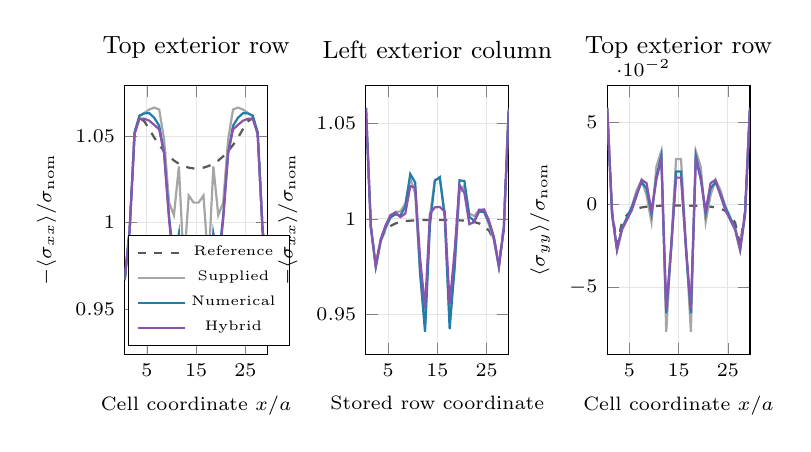
\begin{tikzpicture}
\begin{groupplot}[group style={group size=3 by 1,horizontal sep=1.25cm},width=.28\linewidth,height=5cm,grid=major,grid style={black!10},xmin=.5,xmax=29.5,xtick={5,15,25},tick label style={font=\scriptsize},label style={font=\scriptsize},title style={font=\small},legend style={font=\tiny,at={(.02,.03)},anchor=south west}]
\nextgroupplot[title={Top exterior row},xlabel={Cell coordinate $x/a$},ylabel={$-\langle\sigma_{xx}\rangle/\sigma_{\rm nom}$}]
\addplot[black!65,dashed,thick] coordinates {(0.5,0.966844731) (1.5,0.9959925671) (2.5,1.052048634) (3.5,1.060460339) (4.5,1.058484591) (5.5,1.053909666) (6.5,1.049158468) (7.5,1.044902737) (8.5,1.041288218) (9.5,1.038305687) (10.5,1.035908059) (11.5,1.034047063) (12.5,1.032683575) (13.5,1.031789407) (14.5,1.031346646) (15.5,1.031346646) (16.5,1.031789407) (17.5,1.032683575) (18.5,1.034047063) (19.5,1.035908059) (20.5,1.038305687) (21.5,1.041288218) (22.5,1.044902737) (23.5,1.049158468) (24.5,1.053909666) (25.5,1.058484591) (26.5,1.060460339) (27.5,1.052048634) (28.5,0.9959925671) (29.5,0.966844731)};
\addlegendentry{Reference}
\addplot[black!35,thick] coordinates {(0.5,0.9668388107) (1.5,0.995682149) (2.5,1.051737662) (3.5,1.061527095) (4.5,1.063425723) (5.5,1.065379441) (6.5,1.066485381) (7.5,1.065373484) (8.5,1.048146336) (9.5,1.011595035) (10.5,1.004349522) (11.5,1.032475413) (12.5,0.9747636276) (13.5,1.015680943) (14.5,1.011591494) (15.5,1.011591494) (16.5,1.015680943) (17.5,0.9747636276) (18.5,1.032475413) (19.5,1.004349522) (20.5,1.011595035) (21.5,1.048146336) (22.5,1.065373484) (23.5,1.066485381) (24.5,1.065379441) (25.5,1.063425723) (26.5,1.061527095) (27.5,1.051737662) (28.5,0.995682149) (29.5,0.9668388107)};
\addlegendentry{Supplied}
\addplot[numblue,thick] coordinates {(0.5,0.9668416613) (1.5,0.9958436265) (2.5,1.052105864) (3.5,1.06187376) (4.5,1.063132274) (5.5,1.063185529) (6.5,1.060608458) (7.5,1.055978242) (8.5,1.040247932) (9.5,1.003810962) (10.5,0.9775594149) (11.5,0.9936999086) (12.5,0.9374943964) (13.5,0.9629592426) (14.5,0.9615175125) (15.5,0.9615175125) (16.5,0.9629592426) (17.5,0.9374943964) (18.5,0.9936999086) (19.5,0.9775594149) (20.5,1.003810962) (21.5,1.040247932) (22.5,1.055978242) (23.5,1.060608458) (24.5,1.063185529) (25.5,1.063132274) (26.5,1.06187376) (27.5,1.052105864) (28.5,0.9958436265) (29.5,0.9668416613)};
\addlegendentry{Numerical}
\addplot[agentpurple,thick] coordinates {(0.5,0.9668339475) (1.5,0.9954846486) (2.5,1.051167315) (3.5,1.060028099) (4.5,1.060007056) (5.5,1.058885216) (6.5,1.056467501) (7.5,1.053882432) (8.5,1.039902971) (9.5,1.001983146) (10.5,0.9732570157) (11.5,0.9892819966) (12.5,0.9369144178) (13.5,0.963964431) (14.5,0.9608388713) (15.5,0.9608388713) (16.5,0.963964431) (17.5,0.9369144178) (18.5,0.9892819966) (19.5,0.9732570157) (20.5,1.001983146) (21.5,1.039902971) (22.5,1.053882432) (23.5,1.056467501) (24.5,1.058885216) (25.5,1.060007056) (26.5,1.060028099) (27.5,1.051167315) (28.5,0.9954846486) (29.5,0.9668339475)};
\addlegendentry{Hybrid}
\nextgroupplot[title={Left exterior column},xlabel={Stored row coordinate},ylabel={$-\langle\sigma_{xx}\rangle/\sigma_{\rm nom}$}]
\addplot[black!65,dashed,thick] coordinates {(0.5,1.057941005) (1.5,0.9959925671) (2.5,0.9760366349) (3.5,0.9891021265) (4.5,0.9938211194) (5.5,0.9963002713) (6.5,0.9976156793) (7.5,0.9983584587) (8.5,0.9987994395) (9.5,0.999071421) (10.5,0.9992433789) (11.5,0.9993530443) (12.5,0.9994218621) (13.5,0.9994621788) (14.5,0.9994808138) (15.5,0.9994808138) (16.5,0.9994621788) (17.5,0.9994218621) (18.5,0.9993530443) (19.5,0.9992433789) (20.5,0.999071421) (21.5,0.9987994395) (22.5,0.9983584587) (23.5,0.9976156793) (24.5,0.9963002713) (25.5,0.9938211194) (26.5,0.9891021265) (27.5,0.9760366349) (28.5,0.9959925671) (29.5,1.057941005)};
\addplot[black!35,thick] coordinates {(0.5,1.058213961) (1.5,0.995682149) (2.5,0.9745817636) (3.5,0.9878584197) (4.5,0.9949026368) (5.5,1.000798052) (6.5,1.003668877) (7.5,1.003890417) (8.5,1.008158992) (9.5,1.021316021) (10.5,1.01327711) (11.5,0.970981486) (12.5,0.9435658756) (13.5,1.001538307) (14.5,1.020500046) (15.5,1.021063195) (16.5,1.003486157) (17.5,0.9458787361) (18.5,0.9736097572) (19.5,1.013773235) (20.5,1.017488894) (21.5,1.002797381) (22.5,1.00147315) (23.5,1.00491336) (24.5,1.003449572) (25.5,0.9968396902) (26.5,0.9885789451) (27.5,0.9745743087) (28.5,0.9953857112) (29.5,1.057753792)};
\addplot[numblue,thick] coordinates {(0.5,1.058055539) (1.5,0.9958436265) (2.5,0.9752452047) (3.5,0.9888153336) (4.5,0.9956817922) (5.5,1.000790921) (6.5,1.002447477) (7.5,1.001611408) (8.5,1.006668697) (9.5,1.023467806) (10.5,1.019049568) (11.5,0.9721056954) (12.5,0.9409067977) (13.5,0.9967262581) (14.5,1.019910247) (15.5,1.021865401) (16.5,1.000917185) (17.5,0.9423599402) (18.5,0.9747101853) (19.5,1.020182258) (20.5,1.019790906) (21.5,1.001073458) (22.5,0.9989965073) (23.5,1.003772612) (24.5,1.003776799) (25.5,0.9980322633) (26.5,0.9898115605) (27.5,0.9751856028) (28.5,0.9951045537) (29.5,1.057094398)};
\addplot[agentpurple,thick] coordinates {(0.5,1.057460334) (1.5,0.9954846486) (2.5,0.9754014504) (3.5,0.9894678096) (4.5,0.9967278762) (5.5,1.00203738) (6.5,1.003358784) (7.5,1.00094043) (8.5,1.002775726) (9.5,1.017129901) (10.5,1.016451283) (11.5,0.9795804141) (12.5,0.9533878648) (13.5,1.002669627) (14.5,1.006033265) (15.5,1.00621133) (16.5,1.003848308) (17.5,0.9554321991) (18.5,0.9829765705) (19.5,1.017783036) (20.5,1.013537257) (21.5,0.9972430313) (22.5,0.9983379955) (23.5,1.00463258) (24.5,1.004946199) (25.5,0.9990189609) (26.5,0.9904415109) (27.5,0.9753547182) (28.5,0.9947856002) (29.5,1.056543912)};
\nextgroupplot[title={Top exterior row},xlabel={Cell coordinate $x/a$},ylabel={$\langle\sigma_{yy}\rangle/\sigma_{\rm nom}$}]
\addplot[black!65,dashed,thick] coordinates {(0.5,0.05838616605) (1.5,-0.00418919935) (2.5,-0.02410947359) (3.5,-0.01095002453) (4.5,-0.006202842527) (5.5,-0.00371265542) (6.5,-0.002392146049) (7.5,-0.001646723225) (8.5,-0.001204251676) (9.5,-0.0009313760656) (10.5,-0.0007588590264) (11.5,-0.0006488363859) (12.5,-0.0005797923912) (13.5,-0.0005393416191) (14.5,-0.0005206440138) (15.5,-0.0005206440138) (16.5,-0.0005393416191) (17.5,-0.0005797923912) (18.5,-0.0006488363859) (19.5,-0.0007588590264) (20.5,-0.0009313760656) (21.5,-0.001204251676) (22.5,-0.001646723225) (23.5,-0.002392146049) (24.5,-0.00371265542) (25.5,-0.006202842527) (26.5,-0.01095002453) (27.5,-0.02410947359) (28.5,-0.00418919935) (29.5,0.05838616605)};
\addplot[black!35,thick] coordinates {(0.5,0.05816013898) (1.5,-0.006154149088) (2.5,-0.02793483667) (3.5,-0.01554739283) (4.5,-0.008876885172) (5.5,-0.001050543983) (6.5,0.008901742468) (7.5,0.01491942382) (8.5,0.005840761289) (9.5,-0.01057697795) (10.5,0.02316002538) (11.5,0.03253047626) (12.5,-0.07713981124) (13.5,-0.02398837122) (14.5,0.02775640015) (15.5,0.02775640015) (16.5,-0.02398837122) (17.5,-0.07713981124) (18.5,0.03253047626) (19.5,0.02316002538) (20.5,-0.01057697795) (21.5,0.005840761289) (22.5,0.01491942382) (23.5,0.008901742468) (24.5,-0.001050543983) (25.5,-0.008876885172) (26.5,-0.01554739283) (27.5,-0.02793483667) (28.5,-0.006154149088) (29.5,0.05816013898)};
\addplot[numblue,thick] coordinates {(0.5,0.05830714005) (1.5,-0.005768251964) (2.5,-0.02711910111) (3.5,-0.0143518942) (4.5,-0.007878046287) (5.5,-0.001447129664) (6.5,0.006541638146) (7.5,0.01355707634) (8.5,0.009941608189) (9.5,-0.005625162307) (10.5,0.01700038562) (11.5,0.02971580742) (12.5,-0.06584192125) (13.5,-0.02716813472) (14.5,0.02013598592) (15.5,0.02013598592) (16.5,-0.02716813472) (17.5,-0.06584192125) (18.5,0.02971580742) (19.5,0.01700038562) (20.5,-0.005625162307) (21.5,0.009941608189) (22.5,0.01355707634) (23.5,0.006541638146) (24.5,-0.001447129664) (25.5,-0.007878046287) (26.5,-0.0143518942) (27.5,-0.02711910111) (28.5,-0.005768251964) (29.5,0.05830714005)};
\addplot[agentpurple,thick] coordinates {(0.5,0.05889896826) (1.5,-0.005244095352) (2.5,-0.02695631359) (3.5,-0.01484181376) (4.5,-0.009276814547) (5.5,-0.003328494425) (6.5,0.00565195106) (7.5,0.01506949314) (8.5,0.01307887104) (9.5,-0.00399969219) (10.5,0.01532216767) (11.5,0.02787652488) (12.5,-0.06332316981) (13.5,-0.02533852555) (14.5,0.01641094337) (15.5,0.01641094337) (16.5,-0.02533852555) (17.5,-0.06332316981) (18.5,0.02787652488) (19.5,0.01532216767) (20.5,-0.00399969219) (21.5,0.01307887104) (22.5,0.01506949314) (23.5,0.00565195106) (24.5,-0.003328494425) (25.5,-0.009276814547) (26.5,-0.01484181376) (27.5,-0.02695631359) (28.5,-0.005244095352) (29.5,0.05889896826)};
\end{groupplot}\end{tikzpicture}
\caption{Gross-area stress profiles averaged over original $50\times50$-element cells in the fixed exterior region. Top row index 1 and left column index 1 are used; displayed coordinates are cell centers and stored row increases downward. The profiles retain the original material/void interpolation and are not reoptimized curves. The numerical profile CSV and stress-recovery checks accompany the figures.}
\label{fig:stressprofiles}
\end{figure}
\subsection{Numerical verification}
The monitored reference displacement reconstructed from the supplied uniform base-cell structure agrees with the supplied target to relative difference $1.2912\times10^{-10}$. Small independently assembled models verify the full/half symmetry relation and stiffness assembly. The macro-adjoint derivative check validates the implemented infinitesimal macro derivative, not the accuracy of finite candidate scores. Table~\ref{tab:verification} collects checks at their actual scope.

\begin{table}[htbp]
\centering\small
\caption{Verification evidence. Numerical agreement does not establish physical model validity.}
\label{tab:verification}
\begin{tabular}{@{}p{.65\linewidth}r@{}}\toprule
Check & Recorded discrepancy\\\midrule
Supplied monitored reference, relative difference & $1.29\times10^{-10}$\\
Small-model half/full displacement, relative difference & $1.10\times10^{-15}$\\
Independent triplet stiffness, maximum entry difference & $4.44\times10^{-16}$\\
Small scalar-adjoint finite difference, relative difference & $2.38\times10^{-10}$\\
Macro-adjoint finite difference, relative difference & $2.37\times10^{-7}$\\
Largest free-force residual among 60 candidates & $1.66\times10^{-11}$\\
Final independent free-force residual, numerical / hybrid & $2.33/2.31\times10^{-11}$\\
Final net-force imbalance, numerical / hybrid & $1.95/1.94\times10^{-10}$\\\bottomrule
\end{tabular}
\end{table}

The audit checks 30 distinct new assignments per arm, no cached new proposal evaluations, valid label changes, strict retention, all 20 proposal commitment hashes, identical prior ledgers, and unchanged scientific solver, feedback, and numerical-selector source hashes. Final support reactions and element internal forces are recomputed independently of the forward residual report. No candidate is rejected for force residual; mechanically unsuccessful candidates are rejected because their loss is higher.

Recorded candidate solve-and-refinement times range from 39.05 to 55.67 seconds. Summed times are 1,431.27 seconds for numerical and 1,472.46 seconds for hybrid candidate solves. These exclude AMG setup, feedback formation, agent interaction, and proposal-search overhead; they are not end-to-end optimization times and do not support a speedup claim.

\section{Discussion}
\subsection{A useful role for language agents}
The observed benefit is the construction and revision of experiments in a discrete physical action space. Agents can connect a failed composition to a smaller test, compare a transferred block with its contextual alternatives, and ask whether extending a compatible band remains beneficial. Their output is a concrete action list that can be checked and evaluated. Mechanical predictions still come from numerical models, and acceptance still comes from fine equilibrium.

The hybrid is consequently a tool-using search system, not language-only mechanics. The numerical proposer is integral to its evidence interface and supplies useful comparisons even when a specialist provides the retained design. Conversely, the lower final hybrid loss is not explained by a language model having solved equilibrium implicitly. The initial failed beam repair and failed cloak proposals show why measured retention remains necessary.

\subsection{What the comparison establishes}
The matched new-FEM budget and common historical ledger support a concrete finding: this coordinated hybrid produces a lower final loss than this frozen adaptive numerical portfolio on the supplied case. Both methods improve substantially, and the hybrid's final geometry remains connected at a similar reported material fraction. The result warrants further evaluation of the coordination strategy.

It does not isolate coordination as a single causal factor. There is no new 30-evaluation uncoordinated swarm control, no repeated-team distribution, and no optimizer portfolio exhaustive enough to represent numerical search generally. The preliminary nine-evaluation swarm is not such a control: it uses a smaller budget and different history. The comparison is also not an LLM-versus-GNN test. A larger agent count is not evaluated in this paper.

\subsection{Feedback fidelity and adaptive hypotheses}
Macro gradients are cheap but can misrank finite topology changes. Signed empirical calibration partly addresses this in the numerical policy. The specialists additionally use spatial and contextual reasoning, including proposals with adverse macro scores when earlier measurements justify exploration. Their failures remain essential evidence: a good interface pattern cannot be extended indefinitely, and a helpful cell in one assembly need not help another.

Strong numerical alternatives could use empirical interaction models, contextual bandits, trust-region optimization with richer local surrogates, or systematic subset tests. Those are appropriate next comparators. The present record makes such comparisons possible without attributing all useful adaptation uniquely to language models.

\section{Limitations and future work}
The primary study uses one supplied cavity, one set of 15 candidates at each active cell, one loading case, and one assistant-mediated run. The exact language-model snapshot and decoding settings were not recorded sufficiently for regeneration of the specialist decisions. Literal actions and FEM outcomes are reproducible more directly than the decision process. Prior conversational familiarity further prevents treating this as a held-out test, despite the shared historical ledger.

The original legacy stiffness scaling and nearly void phase are preserved. Agreement with the supplied reference and small force residuals verify reproduction of the numerical problem, not its conditioning under every perturbation or its physical calibration. A cloak void-stiffness sensitivity study, mesh convergence study, nonlinear analysis, multiple-load tests, and fabrication experiments have not been performed. The earlier beam regularization check cannot be transferred as evidence for cloak robustness.

Future work should use multiple cavities and compatible regenerated targets, fixed model and decoding records, repeated runs, explicit wall-clock and token costs, and manufacturing constraints such as minimum ligament width. A matched uncoordinated hybrid control and a stronger numerical search with the same ablation capabilities would help determine which coordination elements add value. A trained GNN comparator requires a separate controlled training and evaluation protocol.

\section{Conclusion}
Coordinated language agents can participate in discrete metamaterial assembly when paired with numerical proposal tools and fine mechanical validation. In the supplied mechanical-cloaking case, the hybrid lowers masked displacement loss from 12.7610\% to 10.6946\%, while an adaptive numerical portfolio reaches 11.6308\% under the same 30-new-evaluation budget and shared historical evidence. Measured compositions, interface extensions, and matched ablations provide concrete examples of how the roles work together. The result is evidence for this implemented hybrid on this case, with generalization and the causal contribution of coordination remaining open.

\section*{Data and code availability}
The public unit-cell library is available under CC BY 4.0 at the Figshare DOI in Ref.~\cite{dataset}. The repository \href{https://github.com/BaratiLab/Metamaterial-Swarm}{BaratiLab/Metamaterial-Swarm} contains the project source, recorded actions, outcomes, validation, figure sources, and manuscript. It is private at preparation; this is an access-controlled working record rather than an independently archived public release. The author-supplied cloak input package is required separately and is not redistributed. Public release permissions and a permanent archived identifier remain to be resolved before journal submission.

\section*{AI assistance and author declarations}
Language agents generated experimental proposals and assisted with code and manuscript preparation. Their nominations are evaluated research objects, not independent human reviews. The human authors must review the code, numerical interpretation, and final scientific claims. The author order and corresponding-author designation are specified above. Detailed contribution, funding, and competing-interest statements must be completed and approved by the listed authors before submission.

\appendix
\section{Supporting beam study}
The earlier beam pilot uses the same public library but a different task, feedback interface, and protocol. A $30\times4$ macro-cell beam has ten candidates per cell and a fine model with 300,000 Q4 elements. It targets the achieved displacement profile of a continuous macro design, sampled on both outer edges. It is paper-inspired rather than an exact reproduction of Ref.~\cite{wang2020}: the library size, constituent Poisson's ratio, loading conventions, and assembly solver differ.

Independent property matching and multistart graph ICM yield errors of 20.73\% and 9.93\%. An initial top-eight numerical repair reaches 4.86\%, while a single assistant-guided batch using homogenized feedback worsens the graph result to 10.82\%. A subsequent three-specialist proposal competition uses assembled-geometry response sensitivities and reduces the numerical incumbent from 4.862985\% to 3.921978\% after three rounds. The numerical and agent groups receive nine candidate assessments each, but share the retained incumbent. Fixed numerical policies repeat their final three candidates, covering only six unique incumbent/action pairs. This is supporting evidence of feasibility, not an independent matched adaptive-optimizer test.

Unlike the cloak, the beam follow-up imposes connectedness, mean geometric mismatch at most 0.20, mean mechanical mismatch at most 0.35, and volume fraction within 0.015 of the starting value. These conditions are not silently applied to the cloak results. The beam archive retains its complete failed and successful proposals, derivative checks, and a limited ersatz-stiffness sensitivity check.

\section{Preliminary cloak study and provenance}
Before the primary follow-up, separate nine-proposal cloak trajectories reach 12.359447\% for numerical search and 12.540622\% for the swarm, starting from 12.761049\%. Numerical policy development includes signed calibration and trust-update refinements; the prior source and literal actions are preserved. All 18 assessments become the common historical ledger for the primary study. The final numerical selector is frozen before new primary outcomes, and its SHA-256 digest is recorded with the protocol. Preliminary trials are not counted as 18 additional new measurements for either primary arm.

\section{Reproduction and implementation details}
The recorded environment uses Python 3.11, NumPy 1.24.3, SciPy 1.11.1, Numba 0.57.1, and PyAMG 5.0.1. BLAS and OpenMP threads are set to one. The original MATLAB sources and data are unchanged. The full model has not been executed in MATLAB or Octave in this environment. The reported reproduction is the validated Python port.

Source data include both ordinary MAT and MATLAB v7.3/HDF5 files. The adapter restores array ordering, excludes inactive candidate zeros, and reproduces the label-index permutation. Agent actions use zero-based independent-cell and label indices; stored library indices are converted from their MATLAB convention. Retained assignments are exported as MATLAB-compatible \texttt{Label} arrays.

All three proposals in an arm-round are saved before any of its candidate outcomes. Commitment hashes and geometry hashes are retained. Round-one scratch launches initially share a namespace but independently execute their common singleton; later hybrid rounds use an arm-specific namespace. Every one of the 60 new trial records reports an uncached solve. This implementation detail does not change the optimization policy or reported evaluation count.

The literal-action replay script recomputes the saved proposals in a new directory without requesting new language-agent decisions. A complete 60-assessment replay was not redundantly rerun after the completed study. The standalone \texttt{main.tex} embeds the vector overview, result plots, and losslessly compressed RGB structure/stress figures through the PGF PDF backend. No external graphics or bibliography database is required. The original PNG/PDF assets and numerical profile CSV are also supplied for reuse.

\section{All primary candidate outcomes}
Table~\ref{tab:alltrials} preserves all 60 measured candidate losses, including failures. N1, N2, and N3 are the numerical singleton, trust-combination, and diverse-beam policies. In the hybrid, T denotes its numerical-tool singleton, R the response agent, and I the interface agent. All candidates are numerically eligible; lower loss determines retention. Rows are correlated adaptive trials, not independent replicates. Literal actions, predicted scores, force residuals, connectivity, volume, and interface metrics are provided in the computational archive.
\small
\begin{longtable}{@{}rrlrrl@{}}
\caption{Complete primary trial outcomes, grouped by round. Losses are percentages.}\label{tab:alltrials}\\
\toprule Round & Tests & Numerical policy & Loss (\%) & Hybrid loss (\%) & Hybrid role\\\midrule
\endfirsthead
\toprule Round & Tests & Numerical policy & Loss (\%) & Hybrid loss (\%) & Hybrid role\\\midrule
\endhead
\bottomrule\endfoot

1 & 1 & N1 & 12.806256 & 12.806256 & T\\
1 & 2 & N2 & 13.394681 & 12.545021 & R\\
1 & 3 & N3 & 13.432845 & 12.845207 & I\\
2 & 4 & N1 & 12.756484 & 12.542988 & T\\
2 & 5 & N2 & 12.760979 & 12.150600 & R\\
2 & 6 & N3 & 12.782182 & 12.626787 & I\\
3 & 7 & N1 & 12.753608 & 12.229157 & T\\
3 & 8 & N2 & 12.753831 & 11.857962 & R\\
3 & 9 & N3 & 12.753283 & 12.145696 & I\\
4 & 10 & N1 & 12.773296 & 11.934579 & T\\
4 & 11 & N2 & 11.980758 & 11.723329 & R\\
4 & 12 & N3 & 12.509731 & 11.894355 & I\\
5 & 13 & N1 & 12.014813 & 11.736362 & T\\
5 & 14 & N2 & 12.014316 & 11.689923 & R\\
5 & 15 & N3 & 11.945736 & 11.500134 & I\\
6 & 16 & N1 & 11.906258 & 11.431839 & T\\
6 & 17 & N2 & 11.944812 & 11.467508 & R\\
6 & 18 & N3 & 11.944722 & 11.302764 & I\\
7 & 19 & N1 & 11.933854 & 11.236154 & T\\
7 & 20 & N2 & 11.831545 & 11.204944 & R\\
7 & 21 & N3 & 11.838597 & 11.596401 & I\\
8 & 22 & N1 & 11.862486 & 11.237872 & T\\
8 & 23 & N2 & 11.777805 & 10.961472 & R\\
8 & 24 & N3 & 11.787137 & 11.056623 & I\\
9 & 25 & N1 & 11.702361 & 10.899081 & T\\
9 & 26 & N2 & 11.661216 & 10.780012 & R\\
9 & 27 & N3 & 11.711493 & 10.815202 & I\\
10 & 28 & N1 & 11.630822 & 10.817768 & T\\
10 & 29 & N2 & 11.641134 & 10.714262 & R\\
10 & 30 & N3 & 11.641203 & 10.694605 & I\\

\end{longtable}
\normalsize
\begin{thebibliography}{9}
\bibitem{wang2020} L. Wang, Y.-C. Chan, F. Ahmed, Z. Liu, P. Zhu, and W. Chen.
Deep generative modeling for mechanistic-based learning and design of metamaterial systems.
\emph{Computer Methods in Applied Mechanics and Engineering}, 372:113377, 2020.
\href{https://doi.org/10.1016/j.cma.2020.113377}{doi:10.1016/j.cma.2020.113377}.
\bibitem{cloak2022} L. Wang, J. Boddapati, K. Liu, P. Zhu, C. Daraio, and W. Chen.
Mechanical cloak via data-driven aperiodic metamaterial design.
\emph{Proceedings of the National Academy of Sciences}, 119(13):e2122185119, 2022.
\href{https://doi.org/10.1073/pnas.2122185119}{doi:10.1073/pnas.2122185119}.
\bibitem{dataset} L. Wang, J. Boddapati, K. Liu, P. Zhu, C. Daraio, and W. Chen.
\emph{2D orthotropic metamaterial micorstructrue dataset}. Figshare, version 1, 2021. CC BY 4.0.
\href{https://doi.org/10.6084/m9.figshare.17141975.v1}{doi:10.6084/m9.figshare.17141975.v1}.
\bibitem{opro} C. Yang, X. Wang, Y. Lu, H. Liu, Q. V. Le, D. Zhou, and X. Chen.
Large language models as optimizers. \emph{International Conference on Learning Representations}, 2024.
\href{https://proceedings.iclr.cc/paper_files/paper/2024/hash/3339f19c5fcee3ad74502947a32be9e6-Abstract-Conference.html}{Conference proceedings}.
\bibitem{react} S. Yao, J. Zhao, D. Yu, N. Du, I. Shafran, K. Narasimhan, and Y. Cao.
ReAct: Synergizing reasoning and acting in language models.
\emph{International Conference on Learning Representations}, 2023.
\href{https://arxiv.org/abs/2210.03629}{arXiv:2210.03629}.
\bibitem{autogen} Q. Wu et al.
AutoGen: Enabling next-gen LLM applications via multi-agent conversation.
\emph{Conference on Language Modeling}, 2024.
\href{https://arxiv.org/abs/2308.08155}{arXiv:2308.08155}.
\end{thebibliography}
\end{document}
